\documentclass[11pt,          % font size: 11pt or 12pt
               phd,           % degree:    ms or phd
               onehalfspacing % spacing: onehalfspacing or doublespacing
               ]{ncsuthesis}

%%----------------------------------------------------------------------------%%
%%------------------------------ Import Packages -----------------------------%%
%%----------------------------------------------------------------------------%%

\usepackage{booktabs}  % professionally typeset tables
\usepackage{amsmath}%,amssymb,amsfonts}
\usepackage{textcomp}  % better copyright sign, among other things
%\usepackage{xcolor}
\usepackage{lipsum}    % filler text
\usepackage{subfig}    % composite figures
\usepackage{listings}

\usepackage[T1]{fontenc}
\usepackage[latin1]{inputenc}
\usepackage[table, svgnames]{xcolor} 
\usepackage{color} 
\usepackage{url}
\usepackage{graphicx, array, blindtext}
\usepackage[tight,footnotesize]{subfigure}
\usepackage{mdframed}
\usepackage{latexsym}
\usepackage{boxedminipage}
\usepackage{ amssymb }
\usepackage[normalem]{ulem}
\usepackage{flushend}

\usepackage{ocgx}
\usepackage{tikz}
\usetikzlibrary{ocgx}

\usepackage{setspace} 

%http://tex.stackexchange.com/questions/106285/boxed-equation-but-framed-only-some-sides
\newcommand{\professional}[1]{\hspace{-1mm}\setlength\arraycolsep{1pt}
	$\begin{array}{|l|}\hline\textnormal{#1}\\\hline\end{array}$\xspace
}	
\newcommand{\undergraduate}[1]{\hspace{-1mm}\setlength\arraycolsep{1pt}
	$\begin{array}{l}\textnormal{#1}\\\hline\end{array}$\xspace
}
\newcommand{\graduate}[1]{\hspace{-1mm}\setlength\arraycolsep{1pt}
	$\begin{array}{|l|}\textnormal{#1}\\\hline\end{array}$\xspace
}

\newcommand*{\mybox}[1]{\framebox{#1}}

%%ORTIZ PACKAGES


%%%%%%%%%%%%%%%%%%%%%%%%%%%%%%%%%%%%%%%%%%
%%%%%%%%%%% Old bibliography commands
%%%%%%%%%%%%%%%%%%%%%%%%%%%%%%%%%%%%%%%%%%5
%\usepackage[super,sort&compress,comma,square,authoryear]{natbib} %\cite command %Added by Ortiz

%use the following line with plainnat
%\usepackage[super,sort&compress,comma,square,numbers]{natbib} %\cite command %Added by Ortiz
%\usepackage{natbib}

%\usepackage[style=alphabetic,natbib=true,backend=bibtex
%sorting=nyt,firstinits=true,isbn=false,doi=false,url=false]{biblatex} %couldn't get backend=biber to work

%\usepackage{filecontents}

%\bibliography{Ortiz-thesis2}
%\bibliographystyle{plain}


%%%%%%%%%%%%%%%%%%%%%%%%%%%%%%%%%%%%%%%%%%
%%%%%%%%%%% Hack for alphanumeric bibliography
%%%%%%%%%%%%%%%%%%%%%%%%%%%%%%%%%%%%%%%%%%5
\RequirePackage[
			style=alphabetic,%numeric-comp,%authoryear-comp,%
			sorting=nyt,%ynt					
			hyperref=true, %	
			firstinits=true,%
			backend=bibtex,
			natbib=true,
			url=false,
			isbn=false,
			maxnames=2, %for et al to be used
			maxalphanames=1, %to avoid printing a + for every et al in the abbreviation
			doi=false]{biblatex}		
			

%needed to do et al after two names
%http://tex.stackexchange.com/questions/44048/use-et-al-in-biblatex-custom-style
\renewcommand*{\finalnamedelim}{\addspace\&\space}

%Simplify abbreviation (the default uses either one or two authors and it indicates et al with a +)
%The following five lines make it so that only the first author is used in the abbreviation
%http://tex.stackexchange.com/questions/27956/label-only-from-first-author
\renewcommand*{\labelalphaothers}{}
    \renewcommand*{\intitlepunct}{}
    \DefineBibliographyStrings{german}{in={}}
    \DefineBibliographyStrings{english}{in={}}
    \DeclareNameAlias{sortname}{last-first}
    \DeclareNameAlias{default}{last-first}
	
%\AtEveryCitekey{\ifciteseen{}{\defcounter{maxnames}{99}}} %authoryear			
\DeclareFieldFormat[article,periodical]{volume}{\mkbibbold{#1}}
\makeatletter

\newrobustcmd*{\parentexttrack}[1]{%
  \begingroup
  \blx@blxinit
  \blx@setsfcodes
  \blx@bibopenparen#1\blx@bibcloseparen
  \endgroup}

\AtEveryCite{%
  \let\parentext=\parentexttrack%
  \let\bibopenparen=\bibopenbracket%
  \let\bibcloseparen=\bibclosebracket}

\makeatother
\renewcommand{\cite}[1]{\parencite{#1}}


\renewbibmacro{in:}{%
  \ifentrytype{article}{}{%
  \printtext{\bibstring{in}\intitlepunct}}}
  
\AtEveryBibitem{\clearfield{month}}

\AtEveryBibitem{\clearfield{language}}
%%%%%%%%%%%%%%%%%%%%%%%%%%%%%%%%%%%%%%%%%%%%%

%\addbibresource{Ortiz-thesis2.bib}
%\addbibresource{Ortiz-thesisURL.bib}
\addbibresource{Johnson-thesis.bib}

 \defbibheading{myheading}[BIBLIOGRAPHY]{
 \chapter*{#1}
 %\centerline{\bf{#1}}
 \markboth{#1}{#1}}

%\usepackage{amsmath,amssymb,amsfonts} %amssymb and amsfonts cannot be used in conjunction with mdput
%\usepackage{graphicx,subfig}% Include figure files
\usepackage{dcolumn}% Align table columns on decimal point
\usepackage{bm}% bold math
%\usepackage{hyperref}% add hypertext capabilities
%\usepackage{hypernat}% make hyperref and natbib work together
\usepackage{cancel}
\usepackage{verbatim}% multiline commenting
\usepackage{ifthen}
\usepackage{url}
\usepackage{sectsty}
\usepackage{balance} 
%\usepackage{caption}
\usepackage{graphicx} %eps figures can be used instead
\usepackage{lastpage}
\usepackage{pdfpages}
\usepackage[format=plain,justification=RaggedRight,singlelinecheck=false,font=small,labelfont=bf,labelsep=space]{caption} 
\usepackage{fancyhdr}
\pagestyle{fancy}

%http://tex.stackexchange.com/questions/100817/error-when-using-bc-from-abbrevs-in-caption
%Getting BC
\usepackage{abbrevs}
\usepackage{etoolbox}
\robustify{\DateMark} % after having loaded abbrevs

\usepackage{units} %Needed to solve bug from citation Hydrodynamics in 21/2 dimensions
%see http://www.latex-community.org/viewtopic.php?f=5&t=989

\usepackage[sharp]{easylist} %used for brainstorming purposes 
%\usepackage{mathabx} % used for \Asterisk for convolution %conflicts with \widering

%compile on single pass
%\usepackage[backend=biber,...]{biblatex}


%%%%%%%%%%%%
%%% Hack to make chapters start on odd pages
% http://tex.stackexchange.com/questions/73591/how-to-have-a-blank-even-page-before-every-chapter
%%%%%%%%%%%%
%\newcommand{\ensureoddstart}{\checkoddpage\ifoddpage\else\newpage\mbox{}\fi}
%\newcommand{\ensureoddstart}{}


%%%Fancy tables
%http://tex.stackexchange.com/questions/94032/fancy-tables-in-latex
\usepackage[table]{xcolor}
\usepackage{array,booktabs}
% \usepackage{colortbl}
\newcolumntype{L}{@{}>{\kern\tabcolsep}l<{\kern\tabcolsep}}



%%%%%%%%%%
%%%%% Hack to allow more levels in outline
%%%%%%%%%%
%\setcounter{secnumdepth}{5}
%\setcounter{tocdepth}{5} %may violate ETD
%Usage http://pleasemakeanote.blogspot.com/2010/06/how-to-activate-subsubsubsection-in.html
%\section{} % level 1
%\subsection{} % level 2
%\subsubsection{} % level 3
%\paragraph{} % level 4 - equivalent to subsubsubsection
%\subparagraph{} % level 5

%http://tex.stackexchange.com/questions/60209/how-to-add-an-extra-level-of-sections-with-headings-below-subsubsection
\usepackage{titlesec}

\setcounter{secnumdepth}{4}

\titleformat{\paragraph}
{\normalfont\normalsize\bfseries}{\theparagraph}{1em}{}
\titlespacing*{\paragraph}
{0pt}{3.25ex plus 1ex minus .2ex}{1.5ex plus .2ex}

%%%%%%%%%%%%%%%%%%%%%%%%%%
%%%% Hack for containing figures within sections
%%%%%%%%%%%%%%%%%%%%%%%%%%%%
%http://ctan.org/pkg/placeins
\usepackage{placeins}
%De�fines a \FloatBar�rier com�mand, be�yond which floats may not pass; use�ful, for ex�am�ple, to en�sure all floats for a sec�tion ap�pear be�fore the next \sec�tion com�mand.

%%%Hack for centering all figures
%\makeatletter
%\g@addto@macro\@floatboxreset\centering
%\makeatother

%%----------------------------------------------------------------------------%%
%%---------------------------- Formatting Options ----------------------------%%
%%----------------------------------------------------------------------------%%
%%

%% -------------------------------------------------------------------------- %%
%% Disposition format -- any titles, headings, section titles
%%  These formatting commands affect all headings, titles, headings,
%%  so sizing commands should not be used here.
%%  Formatting options to consider are
%%     +  \sffamily - sans serif fonts.  Dispositions are often typeset in
%%                    sans serif, so this is a good option. 
%%     +  \rmfamily - serif fonts
%%     +  \bfseries - bold face
%\dispositionformat{\sffamily\bfseries}   % bold and sans serif
\dispositionformat{\bfseries}            % bold and serif

%% -------------------------------------------------------------------------- %%
%% Formatting for centered headings - Abstract, Dedication, etc. headings
%%  This is where one might put a sizing command.
%%  \MakeUppercase can be used to typeset all headings in uppercase.
\headingformat{\large\MakeUppercase}   % All letters uppercase
%\headingformat{\large}                % Not all uppercase
%\headingformat{\Large\scshape}        % Small Caps, used with serif fonts.

%% Typographers recommend using a normal inter-word space after
%% sentences. TeX's default is to add an wider space, but \frenchspacing
%% gives a normal spacing. Comment out the following line if you prefer
%% wider spaces between sentences.
\frenchspacing


%% -------------------------------------------------------------------------- %%
%%  Optional packages
%%    A number of compatible packages to improve the look and feel of
%%    your document are available in the file optional.tex 
%%    (For example, hyperlinks, fancy chapter headings, and fonts)
%% To use these options, uncomment the next line and see optional.tex
%%  Optional Packages to consider.   These packages are compatible with
%%    ncsuthesis.  

%% -------------------------------------------------------------------------- %%
%% Fancy chapter headings
%%  available options: Sonny, Lenny, Glenn, Conny, Rejne, Bjarne
%\usepackage[Sonny]{fncychap}
\usepackage[Rejne]{fncychap}

%%----------------------------------------------------------------------------%%
%% Hyperref package creates PDF metadata and hyperlinks in Table of Contents
%%  and citations.  Based on feedback from the NCSU thesis editor, 
%%  the links are not visually distinct from normal text (i.e. no change
%%  in color or extra boxes).
\usepackage[
  pdfauthor={Carlos Pompeyo Ortiz},
  pdftitle={Rigidity of Microsphere Heaps},
  pdfcreator={pdftex},
  pdfsubject={NC State ETD Thesis},
  pdfkeywords={microfluidics, hard sphere, jamming, suspension, rigidity, friction, microscopy},
  colorlinks=true,
  linkcolor=black,
  citecolor=black,
  filecolor=black,
  urlcolor=black,
]{hyperref}


%% -------------------------------------------------------------------------- %%
%% Microtype - If you use pdfTeX to compile your thesis, you can use
%%              the microtype package to access advanced typographic
%%              features.  By default, using the microtype package enables
%%              character protrusion (placing glyphs a hair past the right 
%%              margin to make a visually straighter edge)
%%              and font expansion (adjusting font width slightly to get 
%%              more favorable justification).
%%              Using microtype should decrease the number of lines
%%              ending in hyphens.
\usepackage{microtype}


%%----------------------------------------------------------------------------%%
%% Fonts 

%% ETD guidelines don't specify the font.  You can enable the fonts
%%  by uncommenting the appropriate lines.  Using the default Computer 
%%  Modern fonts is *not* required.  A few common choices are below.
%%  See http://www.tug.dk/FontCatalogue/ for more options.

%% Serif Fonts -------------------------------------------------
%%  The four serif fonts listed here (Utopia, Palatino, Kerkis,
%%  and Times) all have math support.


%% Utopia
\usepackage[T1]{fontenc}
\usepackage[adobe-utopia]{mathdesign}

%% Palatino
%\usepackage[T1]{fontenc}
%\usepackage[sc]{mathpazo}
%\linespread{1.05}

%% Kerkis
%\usepackage[T1]{fontenc}
%\usepackage{kmath,kerkis}

%% Times
%\usepackage[T1]{fontenc}
%\usepackage{mathptmx}


%% Sans serif fonts -------------------------

%\usepackage[scaled]{helvet}  % Helvetica
%\usepackage[scaled]{berasans} % Bera Sans

%solve bug from fancyhdr in optional
%http://nw360.blogspot.com/2006/11/latex-headheight-is-too-small.html
\setlength{\headheight}{14pt}

%%----------------------------------------------------------------------------%%
%%---------------------------- Content Options -------------------------------%%
%%----------------------------------------------------------------------------%%
%% Size of committee: 3, 4, 5, or 6 -- this number includes the chair
\committeesize{5}

%% Members of committee
%%  Each of the following member commands takes an optional argument
%%   to specify their role on the committee.
%%  For co-chairs, use the commands:
%%      \cochairI{Doug Dodd}
%%      \cochairII{Chris Cox}
%%
\cochairI{Emerson Murphy-Hill}
\cochairII{Sarah Heckman}
\memberI{Tim Menzies}
\memberII{Tiffany Barnes}
\memberIII{Eric Rotenberg}  



%% Student writing thesis, \student{First Middle}{Last}
\student{Brittany Itelia}{Johnson} % a full middle name
%\student{John M.}{Smith} % a middle initial

%% Degree program
\program{Computer Science}

%% Thesis Title
%%  Keep in mind, according to ETD guidelines:
%%    +  Capitalize first letter of important words.
%%    +  Use inverted pyramid shape if title spans more than one line.
%%
%%  Note: To break the title onto multiple lines, use \break instead of \\.
%\thesistitle{A North Carolina State University Sample \LaTeX{} Thesis \break 
%with a Title So Long it Needs a Line Break}
\thesistitle{A Tool (Mis)communication Theory and Adaptive Approach for Supporting Developer Tool Use}

%% Degree year.  Necessary if your degree year doesn't equal the current year.
%\degreeyear{1995}


%%----------------------------------------------------------------------------%%
%%---------------------------- Personal Macros -------------------------------%%
%%----------------------------------------------------------------------------%%

%% A central location to add your favorite macros.

%% A few examples to get you started.
\newcommand{\uv}[1]{\ensuremath{\mathbf{\hat{#1}}}}
\newcommand{\bo}{\ensuremath{\mathbf{\Omega}}}
\newcommand{\eref}[1]{Eq.~\ref{#1}}
\newcommand{\fref}[1]{Fig.~\ref{#1}}
\newcommand{\tref}[1]{Table~\ref{#1}}
\newcommand{\del}{\nabla}
\renewcommand{\exp}[1]{e^{#1}}
\newcommand{\Conv}{\mathop{\scalebox{1.5}{\raisebox{-0.2ex}{$\ast$}}}}%


\usepackage{color}
%\newcommand{\NEW}[1]{\textcolor{blue}{#1}}
\newcommand{\NEW}[1]{#1}
\newcommand{\COMMENT}[1]{\textcolor{green}{#1}}


\newcommand{\NOTER}[1]{\textcolor{orange}{#1}}
\newcommand{\NOTEC}[1]{\textcolor{blue}{#1}}
\newcommand{\NOTEK}[1]{\textcolor{magenta}{#1}}

\newcommand{\mum}{\ensuremath{{\mu}\text{m}}}

%This makes it so that you can add short paths in your .tex by including the folders where you store your images in the search path
\graphicspath{{./Chapter-1/figs/}{./Chapter-2/figs/}{./Chapter-3/figs/}}%{./Chapter-4/figs/}{./Chapter-5/figs/}{./Chapter-6/figs/}}


%%---------------------------------------------------------------------------%%
\usepackage{calc}
%% Capital letter height
\newlength{\chaptercapitalheight}
\settoheight{\chaptercapitalheight}{D}
\newlength{\chapterfootskip}
\setlength{\chapterfootskip}{\chaptercapitalheight}
\addtolength{\chapterfootskip}{2\baselineskip}
\addtolength{\chapterfootskip}{0.5ex}  % A little extra space to ensure there are 2 full double spaced lines
%\def\chapterfootskipnum{\chapterfootskip}
\renewcommand{\listfigurename}{LIST OF FIGURES}
\renewcommand{\listtablename}{LIST OF TABLES}
\renewcommand{\bibname}{BIBLIOGRAPHY}

%\renewcommand{\cfttoctitlefont}{\centering\ncsu@headingformat}


%http://tex.stackexchange.com/questions/47184/height-of-figure-caption-textheight
\newlength\graphht
\newcommand\calculategraphicstargetheight[1]{%
     \setlength\graphht{\textheight 
                       -\parskip
                       -\abovecaptionskip -\belowcaptionskip
                       -(12pt * #1) % assuming baselineskip of 12pt in caption
                       -\chapterfootskip
                       }}

%\usepackage{titlesec}

%landscape support in fancyhdr from http://tex.stackexchange.com/questions/9071/how-to-translate-and-rotate-the-heading-of-landscaped-pages
\usepackage{pdflscape}
\usepackage{tikz}
\fancypagestyle{lscapedplain}{%
  \fancyhf{}
  \fancyfoot{%
    \tikz[remember picture,overlay]
      \node[outer sep=1cm,above,rotate=90] at (current page.east) {\thepage};}
\renewcommand{\headrulewidth}{0pt} 
\renewcommand{\footrulewidth}{0pt}
}

                      
\begin{document}
\pagestyle{plain}
%%---------------------------------------------------------------------------%%
\frontmatter

%% ------------------------------ Abstract ---------------------------------- %%
\begin{abstract}
\doublespacing
\noindent Software development and maintenance is an important part of the software engineering process. It is during these phases of the software engineering process that developers complete actions to ensure quality software, such as finding and resolving software defects and refactoring.
Many of the actions involved in writing and maintaining software are manual, tedious and, as a result, error-prone.
Program analysis tools, including those that find and resolve defects, provide feedback to and automate tasks for developers. 
Research has found, however, that developers use these tools infrequently in practice. 
Multiple studies have explored developers' usage of program analysis tools and cumulatively found that developers encounter various challenges when attempting to understand and resolve problems in their code. 

\textit{The goal of this research is to improve the communication between developers and static analysis tools by providing theories and approaches that identify and utilize the differences between developers' information needs, based on their knowledge, that influence developers' ability to resolve tool notifications.}
To achieve this goal, I explored developer tool usage and information needs when understanding and resolving notifications.
In this thesis, I propose a theory that suggests developers have difficulty with tool output because of gaps and mismatches between how much developers know and how tools communicate. I evaluate this theory by building on other existing research to determine factors that influence developer knowledge and information needs of developers, based on their knowledge, when resolving defects.


My thesis consists of a consecution four studies. I first conducted a study to explore the reasons developers have for using and not using static analysis tools. I categorized interview responses from professional developers about their usage of tools and identified five reasons developers have for not frequently using the tools available to them. 
The results suggest that one major barrier to use is the ability for developers to understand the textual and visual notifications provided by tools. 
The second study took a deeper look at the difficulties developers have when understanding tool notifications by observing developers as they attempt to explain textual and visual notifications presented by various tools. Based on the data collected and analyzed, I proposed a theory of tool communication based on the 10 kinds of challenges identified in the data. All of the challenges identified in this study stemmed from gaps in developers' knowledge that notifications did not fill and mismatches between knowledge participants had accrued through their experiences and the information provided by tools.

After determining an explanation for developer difficulties with tool notifications, the next study evaluated the possibility of operationalizing and evaluating that theory. The theory, and previous research, suggests software development experiences influence developer knowledge. Therefore, the third study used developer source code contributions, one of the primary experiences for developers, and concept inventories, a validated educational assessment, to classify developers based on their knowledge of programming concepts.
The models created from this study classified developers' knowledge of variables, exception handling, and generics with 60--80\% accuracy. 
Results from this study support the possibility for tools to automatically ascertain how much developers know about the defects they encounter in their code using the source code they have written. 

Finally, because it is possible can classify developer knowledge using their code contributions, the fourth study evaluated the effectiveness of using developer knowledge classification to customize the information presented to developers by program analysis tools. I used existing research on problem solving to adapt notifications communicating about defects pertaining to the concepts of variables, exception handling, and generics. I presented developers classified as novices and experts in the concepts of interest with notifications aligned and misaligned with their knowledge classification to compare performance and preference. I found that most often, it took participants less time to resolve notifications aligned with their knowledge classification; there was a significant difference between the time it took novices and experts in a given concept to resolve aligned versus misaligned notifications. I also found that on average, novices in a given concept presented with aligned notifications made significantly fewer attempts at resolving notifications than those presented with misaligned notifications, and that developers tended to prefer information provided in aligned notifications. For experts, aligned notifications led to a higher percentage of resolved notifications.
Although not all differences in observations were statistically significant, results from this study suggests that presenting information in tool notifications based on developer software development experiences can improve communication between developers and their tools. 
I conclude this thesis with a discussion of future research directions that will stem from this research.



\end{abstract}


%% ---------------------------- Copyright page ------------------------------ %%
%% Comment the next line if you don't want the copyright page included.
\makecopyrightpage

%% -------------------------------- Title page ------------------------------ %%
\maketitlepage

%% -------------------------------- Dedication ------------------------------ %%
\begin{dedication}
\doublespacing
 \centering To my parents, Engadine and Valerie, who made me the strong black woman I am.
 
 \centering To my sister, Chelsea, who continues to motivate and inspire me through everything.
 
 \centering To the love of my life, Anthony, who has been supportive and by side the whole ride.
 
 \centering To my first mentor, Dr. James Bowring, who helped me find my passion and urged me to pursue it.
\end{dedication}

%% -------------------------------- Biography ------------------------------- %%
\begin{biography}
\doublespacing
Brittany Itelia Johnson was born in a small town called Sumter, South Carolina to Engadine and Valerie Johnson on November 25, 1988. She graduated from Sumter High School in 2007. During her time in high school, Brittany was active in the marching and jazz bands. After high school, she continued on to pursue her undergraduate degree at the College of Charleston (CofC), where she studied Computer Science. 
While at CofC, Brittany was a member of SCAMP, an organization focused on increasing minority participation in STEM research. This led to her participation in undergraduate research, which informed her passion to pursue a Ph.D. She was also a member of the Pep Band, where she let off some academic steam, and an officer in the CofC Chapter of the National Society of Collegiate Scholars.
Brittany obtained her Bachelor of Arts in Computer Science in Spring 2011. She was selected as the feature student graduating from College of Charleston with the Class of 2011 for her involvement and performance in academics, research, and extra-curricular activities. 
Following her time at CofC, Brittany began her journey to her Ph.D. at NC State University in Fall 2011 under the direction of Dr. Emerson Murphy-Hill. As she began her Ph.D. studies, she accrued a co-advisor, Dr. Sarah Heckman. During her time at NC State, aside from her research, she participated in numerous outreach and mentoring initiatives as she discovered her passion for mentoring others like her.  
Brittany aspires to have a career in academia, where she can incorporate both her passion for research and her passion for mentoring.
\end{biography}

%% ----------------------------- Acknowledgements --------------------------- %%
\begin{acknowledgements}
I would like to thank my advisors, my committee, the Developer Liberation Front, RealSearch, and AltCode for their help.
\end{acknowledgements}


\thesistableofcontents

\thesislistoftables

\thesislistoffigures


%%---------------------------------------------------------------------------%%
\mainmatter



\pagestyle{fancy}
\newgeometry{margin=1in,lmargin=1.25in,footskip=\chapterfootskip, includehead, includefoot}
\chapter{Introduction}
\label{chap-one}

Software implementation and maintenance are important parts of the software development process~\cite{krishnan2000empirical}. It is during these phases that developers complete actions to ensure quality software, such finding and resolving software defects and refactoring.
Many of the actions involved in writing and maintaining software are manual, tedious and, as a result, error-prone.
Tools, known as \textit{program analysis tools}, exist for developers to automate some of theses tasks and reduce the effort involved in tasks like defect finding and resolution~\cite{bruckhaus1996impact}. 
Some program analysis tools, known as static analysis tools, allow developers to find and resolve defects early in the development process and occasionally to find defects previously overlooked~\cite{ayewah2010google,Ayewah:2008:FindBugs}.

Research has found, however, that developers use these tools infrequently in practice~\cite{Ayewah:2008:FindBugs, ge2012reconciling, smith2015questions}. 
Multiple studies have explored developers' usage of program analysis tools and cumulatively found that developers encounter various challenges when attempting to understand and resolve problems in their code~\cite{johnson2013don,smith2015questions,christakis2016developers}. 

This dissertation proposes and evaluates the following:

\vspace{0.5em}

\noindent\fbox{\centering
	\parbox{\textwidth}{ \centering
	Program analysis \emph{tool use} is a form of \emph{communication} and \emph{inability to interpret and}\\ \textit{ resolve} notifications is a result of \emph{miscommunication} caused by \emph{knowledge gaps} and \\
	\emph{knowledge mismatches}; therefore we can improve tool design by providing the means for \\tools to \emph{classify} individual developer's \emph{conceptual knowledge} and adapt notifications  \\accordingly, leading to the potential for \emph{reducing time} required for developers to resolve \\tool notifications, \textit{increasing ability to resolve}, and \textit{decreasing attempts made when resolving.}}
	}

\vspace{1em}

To provide concrete motivation for this research, consider Valerie. Valerie is a hypothetical software developer at a start-up company. She primarily writes Java code, though she did not learn to program in Java, and uses the Eclipse Integrated Development Environment (IDE). In her spare time, she builds her knowledge of Java programming concepts by contributing to open source software and using tools that provide feedback about the code she writes. While modifying code in the Sun JDK source code repository, she contributes code that results in the notification shown in Figure~\ref{fig:eclipse}. She has experience using FindBugs, so she is familiar with some of the ways FindBugs communicates. For example, she knows that an orange bug icon indicates a \textit{scary} bug and that by clicking the bug icon she can gain access to more information about the bug.

\begin{figure}
	\centering
	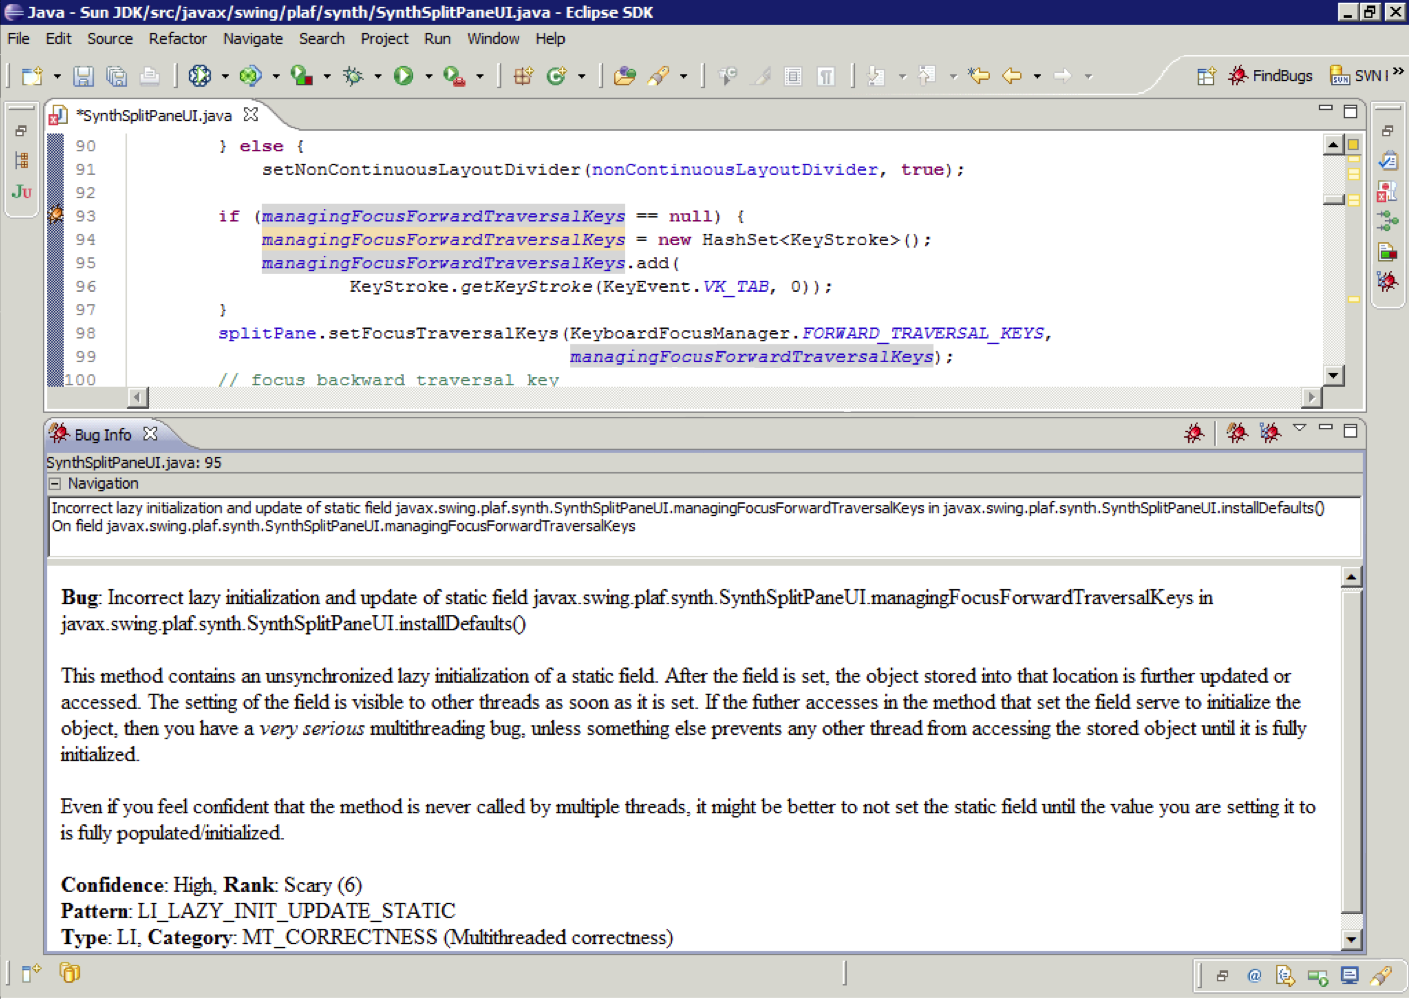
\includegraphics[width=\textwidth]{Chapter-2/figs/eclipse.png}
	\caption{Findbugs notification in the Eclipse IDE concerning multi-threading.}
	\label{fig:eclipse}
\end{figure} 

As she explores the information provided by FindBugs, she realizes that despite her experience with FindBugs, she is having difficulty determining how to resolve the notification. She first attempts to use what knowledge she does have regarding multi-threading, which she accrued from struggling with and resolving compiler synchronization warnings, to better understand the problem. 
% TODO not clear what "the problem" is - be specific
However, she is unfamiliar with the concept central to the notification in Figure~\ref{fig:eclipse} (lazy initialization). Though the notification tells her that the problem relates to multi-threading, she is unable to make a connection between her knowledge regarding multi-threading and the message FindBugs is attempting to communicate and therefore cannot resolve the notification without outside help. As done previously with compiler synchronization notifications, she toggles between the web and her IDE to understand and resolve the notification.

% TODO compiler synchronization notification??

\begin{figure} 
	\centering
	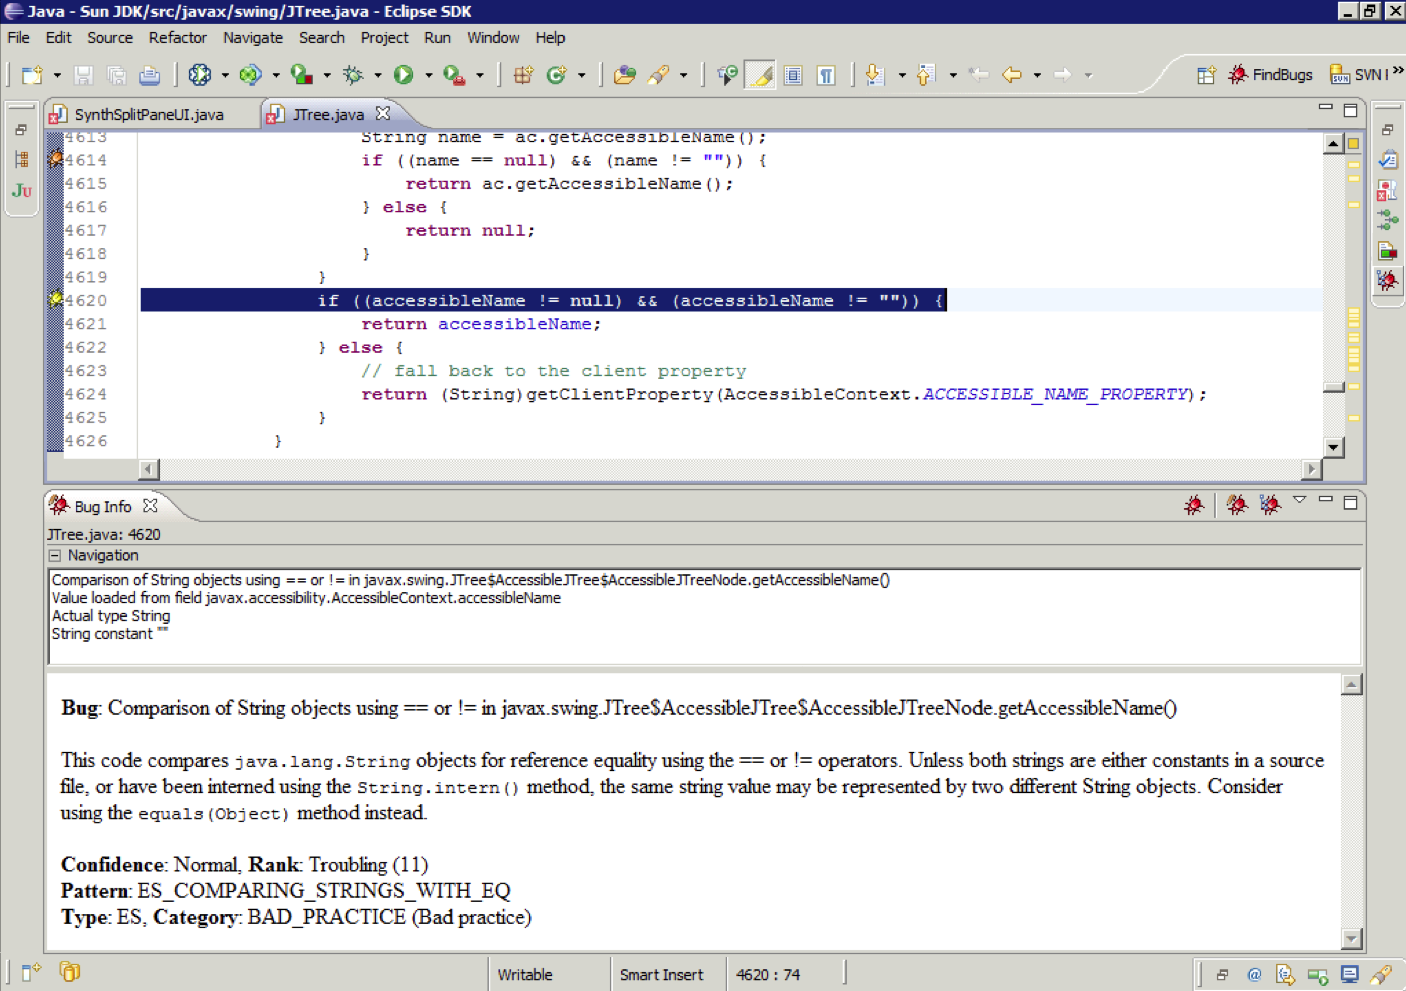
\includegraphics[width=\textwidth]{Chapter-2/figs/eclipse-2.png}
	\caption{Findbugs notification in the Eclipse IDE on checking string equality.}
	\label{fig:eclipse2}
\end{figure}

Although Valerie's goal when using tools like FindBugs is to find and resolve defects, which requires the ability to interpret the notifications provided by the tools, a secondary goal is to learn more about Java programming concepts. She found, however, that some notifications are better at communicating problems while contributing to knowledge than others. For example, when first learning how to work with strings in Java, Valerie encountered the notification in Figure~\ref{fig:eclipse2}. The first time she encountered the problem she was able to understand and resolve the notification. Looking back, she realizes this was because the notification in Figure~\ref{fig:eclipse2} filled in gaps in her own knowledge of the concept by informing her \emph{why} what she was doing was wrong and \emph{how} she can fix it.

Because the tools Valerie uses have no notion of what she does and does not know, some notifications communicate in a way that she is able to understand the problem, while others are not, leading to  miscommunication.
\textit{The goal of this research is to improve how program analysis tools communicate to developers by providing theories and approaches that identify and utilize the differences between developer information needs, based on their knowledge, that influence their ability to resolve tool notifications.}

In the following chapters, I will discuss the research I conducted to explore challenges like those encountered by Valerie and research for developing techniques, frameworks, and tools to mitigate these kinds of challenges.
Chapter~\ref{chap:rw} ground my research in existing research in Computer Science and other fields.
Study 1, outlined in Chapter~\ref{chap:why}, answers the following research questions:
\begin{itemize}
    \item [RQ\textsubscript{1}]: \textit{What reasons do developers have for using or not using static analysis tools to find bugs?}
    \item [RQ\textsubscript{2}]: \textit{How well do current static analysis tools fit into the workflows of developers? We define a workflow as the steps a developer takes when writing, inspecting and modifying their code.}
    \item [RQ\textsubscript{3}]: \textit{What improvements do developers want to see being made to static analysis tools?}
\end{itemize}

Based on findings from Study 1, which identified tool notification understandability as a barrier to use, Chapter~\ref{chap:theory} answers the research question \textit{why do developers encounter challenges when interpreting tool notifications?}.
I used the findings from Study 2 to formulate the boxed explanatory theory above regarding how knowledge affects developers' ability to interpret and resolve notifications.
Using this theory, Chapters~\ref{chap:assess} and~\ref{chap:experience} present Study 3, which answers the following research questions:
\begin{itemize}
    \item [RQ\textsubscript{1}]: \textit{Is source code a good predictor of how much developers know about programming concepts?}
	\item [RQ\textsubscript{2}]: \textit{Does concept-specific source code increase the ability to classify how much developers know about programming concepts in comparison to a naive model?}
\end{itemize}

In Chapter~\ref{chap:assess}, I outline an approach used to assess developer concept knowledge in preparation for the work done in Chapter~\ref{chap:experience} to predict developer concept knowledge.
Finally, based the ability to predict conceptual knowledge, I posit and evaluate the following hypotheses and research question in Chapter~\ref{chap:improve}:
\begin{itemize}
    \item [H\textsubscript{1}]: \textit{Knowledge-based notifications can decrease the time required for notification resolution.}
    \item [H\textsubscript{2}]: \textit{Knowledge-based notifications increase developer likelihood of resolving notifications. }
    \item [H\textsubscript{3}] Knowledge-based notifications decrease developer code churn when resolving notifications.
    \item[RQ]: \textit{Do developer adaptation preferences match expectations from existing problem solving literature?}
\end{itemize}

Findings from Study 4 suggest the possibility of improving developer ability to quickly resolve notifications. Though the differences observed in this study are small, it is a first step in the direction of better understanding how to improve tool use for developers. To conclude this dissertation, Chapter~\ref{chap:future} outlines possible directions for future work that builds the foundations set by this research in this thesis.

The contributions of this dissertation are as follows:
\begin{itemize}
    \item A categorized list of reasons developers have for not using program analysis tools, accompanied by tool design suggestions provided by developers.
    \item An explanatory theory for the challenges that developers encounter when interpreting information provided by tool notifications.
    \item An approach for assessing developer depth of programming concept knowledge that builds on an existing validated approach for assessing breadth of knowledge.
    \item An approach, developed using existing problem solving research, for adapting tool notifications based on developer concept knowledge.
\end{itemize}

\chapter{Related Work}
\label{chap:related}

\section{Program Analysis Tools}
Program analysis tools are designed to aid developers when developing software by automating the writing, analysis, and modification of source code.
Often, program analysis is discussed as synonymous with static analysis~\cite{nielson2015principles}. 
For the purpose of my research, I define a program analysis tool as \emph{a recommendation system that performs program analysis, whether it be static or dynamic analysis, and provides information to develoeprss regarding the source code being analyzed}~\cite{robillard2014recommendation}.
Examples of program analysis tools include, but are not limited to, static code analyzers, code coverage tools, code smell detectors, and refactoring tools~\cite{adolph2011using,Murphy-Hill:2010:Ambient,ge2012reconciling}.
Program analysis tools can be used in integrated development environments (IDEs) as well in most text editors that can be used for programming, such as Vim~\footnote{http://www.vim.org/} or Emacs~\footnote{https://www.gnu.org/software/emacs/}. 
In the following sections, I will define and discuss static analysis and dynamic analysis tools separately; the reader should note that although I discuss static and dynamic analysis separately, it is not uncommon to find program analysis tools that combine static and dynamic analysis~\cite{ernst2003static}.                                                

\subsection{Static Analysis Tools}

Static analysis tools are designed to aide developers when developing software by statically analyzing source code, pre-runtime, and providing the developer with feedback about the state of their code~\cite{ernst2003static}.
Typically, static analysis works by examining the current state of the program, predicting how the program may react in that state at runtime, and reporting any information they deem necessary to the developer. Static analyses are often more conservative than dynamic analyses; this is to reduce the potential for false positives, as in most cases static analysis cannot say with 100\% certainty what will happen during run-time~\cite{ernst2003static}. 
Examples of static analysis tools include defect detectors, such as FindBugs, compilers, code smell detectors, and refactoring tools.
% TODO talk about what static analysis can do/find to motivate further

Let's use the example of FindBugs,\footnote{http://findbugs.sourceforge.net/factSheet.html} an open source static analysis tool, to better understand how static analysis tools work. FindBugs statically analyzes code to report potential defects. FindBugs determines the potential for defects using \emph{bug patterns}. Bug patterns are code idioms that map to errors, found in Java \emph{bytecode}. Bytecode, in Java, represents the compiled Java class files. Because FindBugs analyzes code without executing it, there is a heightened risk for \emph{false positives}. False positives are defects detected that will never manifest during run-time. When FindBugs finds a potential defect, it alerts the developer using notifications that provide information regarding the defect. I will discuss tool notifications in more detail in Section~\ref{subsec:comm}.


\subsection{Dynamic Analysis Tools}

Dynamic analysis tools are designed to aide developers when developing software by analyzing source code during run-time and providing the developer with feedback about runtime behavior~\cite{ernst2003static}.
Dynamic analysis works by executing the program and then making observations about program execution; because dynamic analysis runs the code, it is typically more precise than static analysis. Though dynamic analysis can produce more precise results in a similar amount of time as static analysis, dynamic analysis execution is less likely to generalize to future executions since it is based on a set of inputs that can, and probably will, change for each execution.
Examples of dynamic analysis tools include testing, code coverage, and profiling tools.

Let's use the example of Cobertura,\footnote{http://cobertura.github.io/cobertura/} an open source dynamic code coverage tool, to better understand how dynamic analysis tools work. Cobertura executes source code using JUnit test cases and reports to the user what parts of the code got covered during execution and what parts did not. Because Cobertura executes the source code, it can communicate precisely regarding the flow of the program during run-time. A static code coverage tool could speculate how much of a code base would be covered based on test cases, and possibly even a set of inputs; however, it would require more effort and be more likely to produce false positives than a dynamic code coverage tool. On the down side, the test suites a developer writes may not be characteristic of all possible executions of the program, thereby lowering the generalizability of dynamic analyses.

\begin{figure} [ht]
	\centering
	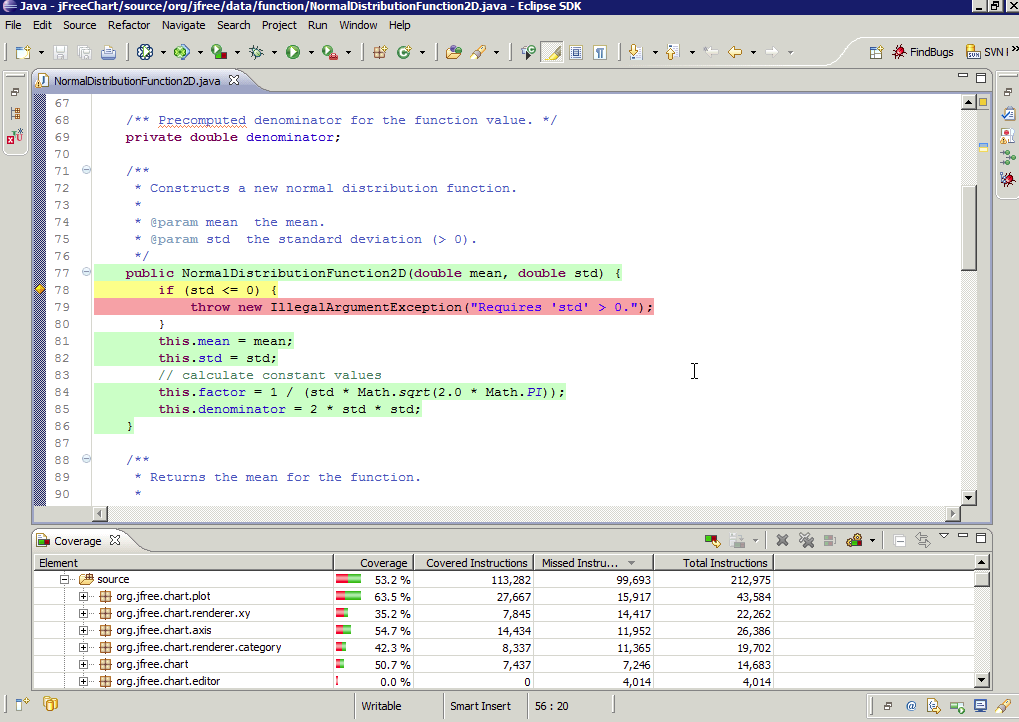
\includegraphics[width=\textwidth]{Chapter-2/figs/eclemma.png}
	\caption{EclEmma notifications in the Eclipse IDE.}
	\label{fig:ecl}
\end{figure}


\subsection{Communication via Notifications}\label{subsec:comm}

One common thread between program analysis tools like FindBugs and Cobertura is that they use \emph{notifications} to communicate with the developer. Figure~\ref{fig:eclipse} and Figure~\ref{fig:ecl} provide examples of tool notifications. 
A notification, when speaking in terms of program analysis tools, is typically a combination of visuals and text used to communicate a message to its user; for program analysis tools, the user is the developer.
Text editors like Vim and Emacs rarely include any visual components, however, because text editors are a simpler versions of IDEs, research on notifications in IDEs are more likely to also apply to text editors than vice versa. 
Therefore, I focus my research on notifications inside IDEs.

Notifications across tools vary; some provide lots of text (like FindBugs) with few visual aides, some use primarily visual means of communications (like Cobertura). Notifications can also have different goals, which may influence how developers design notifications. For example, the goal of a notification from Coverity~\footnote{http://www.coverity.com/}, another static analysis tool, is to explain a potential defect in the developer's source code and, ideally, help the developer make a decision about the defect (i.e. whether and how to resolve). Because Coverity's goal is to explain, we expect to see textual notifications that provide that explanation.
The goal of code coverage notifications is to statically show dynamic program behavior and help the developer determine the effectiveness of her test suite. EclEmma, another code coverage tool, uses colors applied directly to the source code to communicate as opposed to text. Though EclEmma also uses text to communicate code coverage (i.e. \texttt{1 of 2 branches missed} on a partially covered \texttt{if} statement), this does not allow the developer to scan the program for areas in most need of attention. Therefore, EclEmma uses other visuals, such as the bar visuals in the Coverage View (Figure~\ref{fig:ecl}) to show coverage on a given package or class.
 % TODO talk about how different parts of notification communicate for each tool; make sure it ties back to goals (defects and test coverage)!

The list of tools and notifications tools use can go on and on, but for the purposes of my research, the general definition I will use for a notification is \emph{a combination of visual and textual interfaces used by a program analysis tool to communicate information to developers about their source code.} Notifications can vary regarding what information and how much detail they provide, however, there are commonalities across tool notifications that informed this definition, which I will discuss next.

\subsection{Typical Notification Components}
% based on robilliard book
One reason I talk about program analysis tools as a type of recommendation system is because they provide information to developers completing software engineering tasks~\cite{robillard2014recommendation}. 
Another reason is that program analysis tools use the same strategies defined by Robillard as typical of recommendation systems: 1) strategies for getting the user's attention and 2) descriptive interfaces.
Program analysis tools use these strategies when communicating with developers via notifications.

There are a variety of ways that a tool can get the attention of its user~\cite{robillard2014recommendation}. Program analysis tool notifications get the attention of developers in their IDEs in one or more of the following ways: icons, dashboards, pop-ups, affordance overlays, annotations, or email notifications.
Once the tool has the developer's attention, program analysis tool notifications provide descriptive interfaces that convey information about a developer's source code. 
Information is conveyed using some combination of textual, visual, and sometimes transformative descriptions.

Some tools, like FindBugs and most IDE compilers, use icons to get developers' attention. Using the same icons, developers can access more information either by hovering over or clicking the icon. Although the icons are visual, most of the description provided by these tools is textual. As stated previously, these kinds of notifications are most common with static analysis tools as they typically need to be more descriptive. However, dynamic analysis tools like Veracode~\footnote{http://www.veracode.com/products/dynamic-analysis-dast/dynamic-analysis}, which communicate about defects similar to the ones reported by FindBugs and Coverity, also use icons and text descriptions to pass along information to the developer.

\begin{figure}
	\centering
	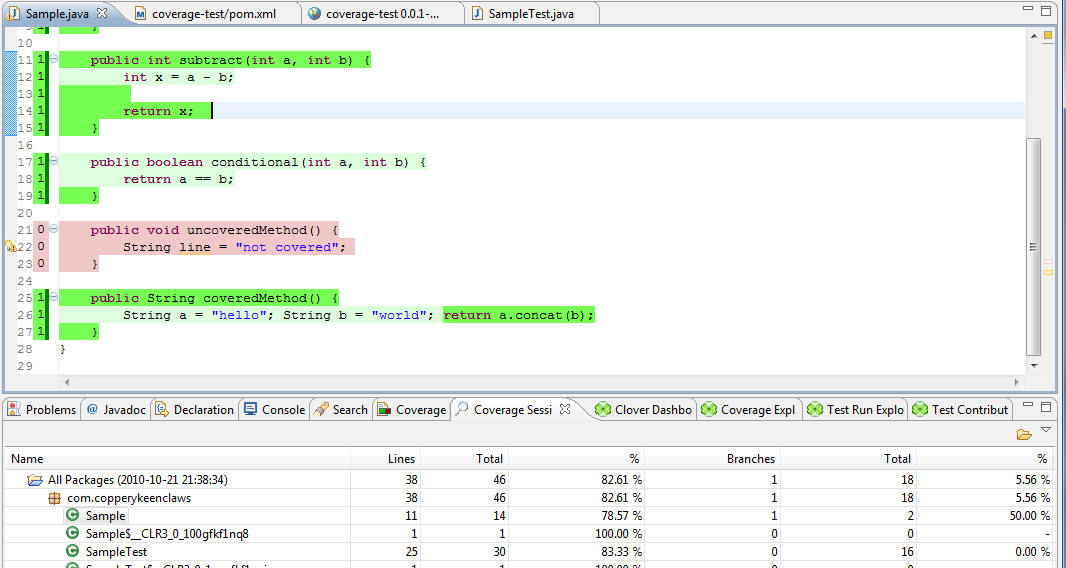
\includegraphics[width=3in]{Chapter-2/figs/cobertura.png}
	\caption{Notifications provided by Cobertura regarding code coverage.}
	\label{fig:cobertura}
\end{figure}

\begin{figure}
	\centering
	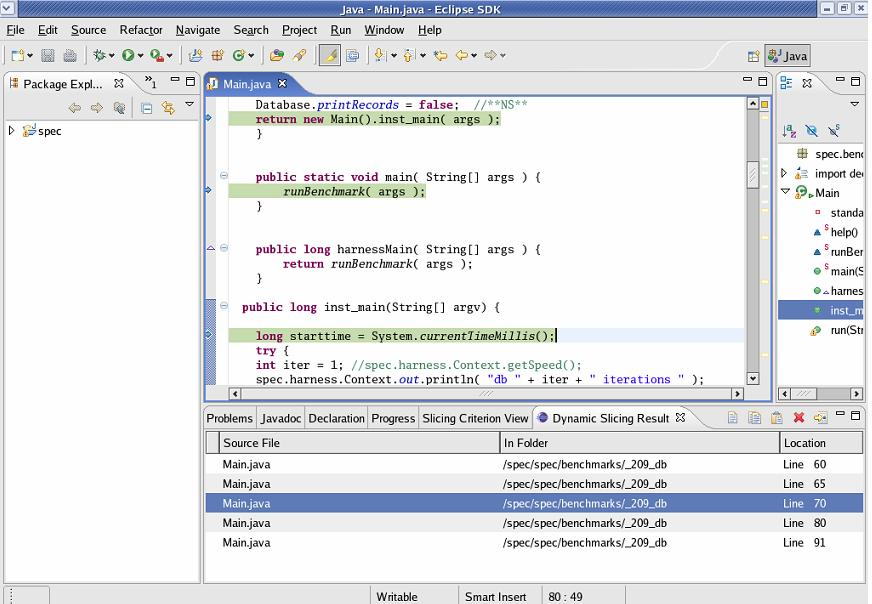
\includegraphics[width=3in]{Chapter-2/figs/jslice.jpg}
	\caption{Notifications provided by JSlice regarding a dynamic slice of the program.}
	\label{fig:jslice}
\end{figure}


Some tools use affordance overlays or annotations to both get the attention of the developer and for the descriptive interface. For example, Cobertura and JSlice~\footnote{http://jslice.sourceforge.net/} use affordance overlays in the form of source code highlighting, as shown in Figure~\ref{fig:cobertura} and Figure~\ref{fig:jslice}, to alert the developer of and communicate about dynamic behavior. Coverity Dynamic Analyzer~\footnote{http://www.coverity.com/library/pdf/Coverity-Dynamic-Analysis.pdf}, which is similar to Veracode, uses annotations, such as the one in Figure~\ref{fig:coverity} in the editor to communicate about defects in the code.

\begin{figure}
	\centering
	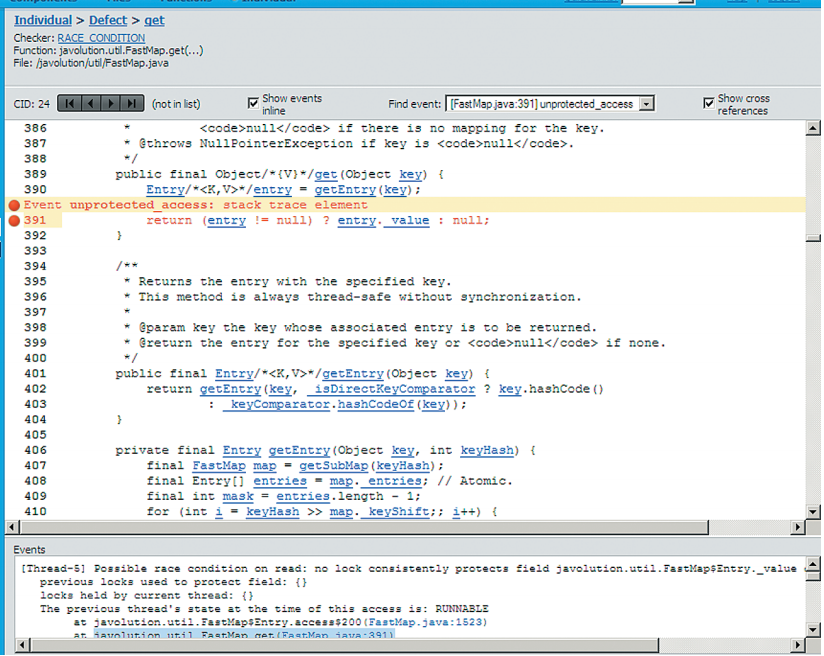
\includegraphics[width=3in]{Chapter-2/figs/coverity-dynamic.png}
	\caption{A notification provided by Coverity regarding a race condition.}
	\label{fig:coverity}
\end{figure}

A small subset of tools use dashboards, such as the one shown to the right in Figure~\ref{fig:stench}. StenchBlossom, a code smell detection tool gets and maintains a developer's attention using an ambient dashboard~\cite{Murphy-Hill:2010:Ambient}. At anytime the developer is interested in the information being provided by the tool, the developer can use options in the dashboard to explore code smells present in their code base. The description is visual, using color overlays that map to each type of code smell. 

\begin{figure}
	\centering
	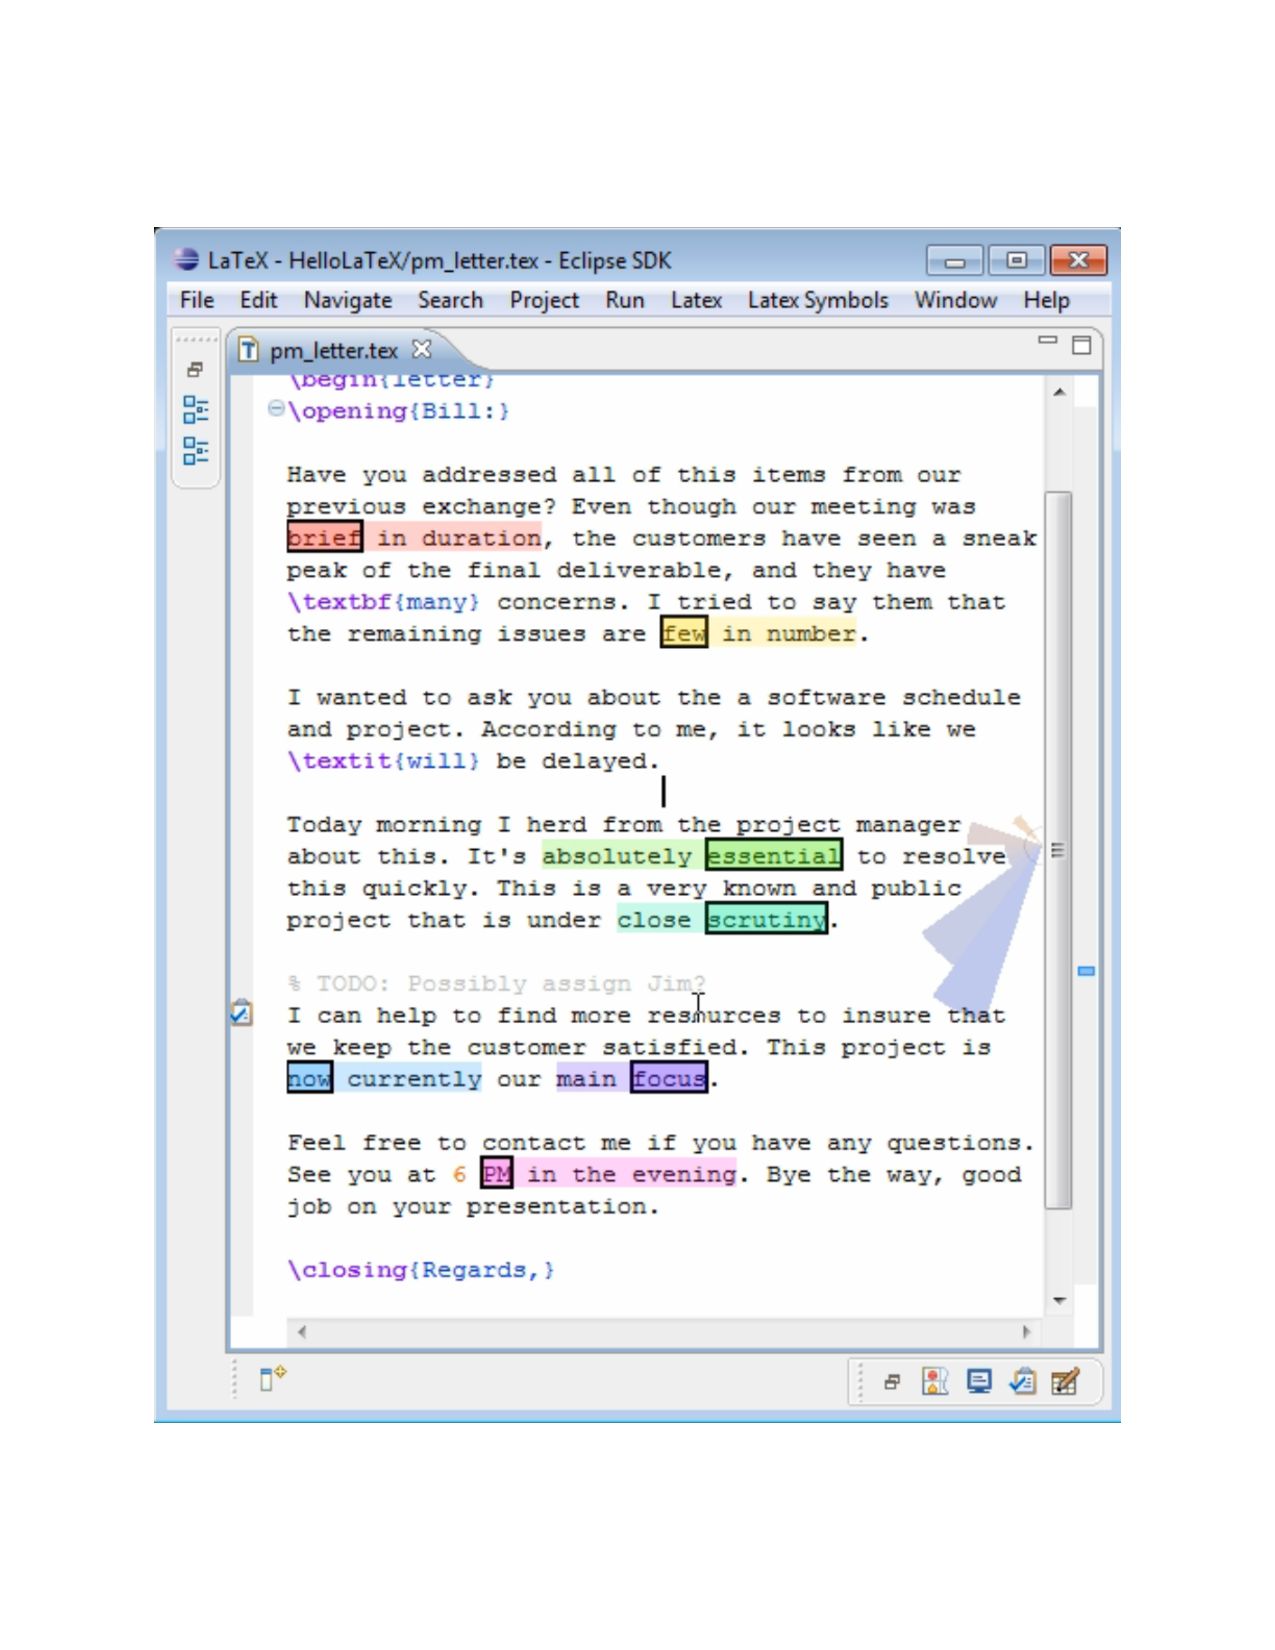
\includegraphics[width=3in]{Chapter-2/figs/stenchblossom.pdf}
	\caption{Notifications provided by StenchBlossom regarding code smells.}
	\label{fig:stench}
\end{figure}

\begin{figure}
	\centering
	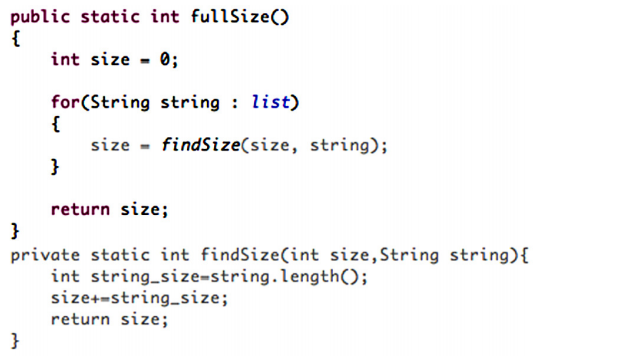
\includegraphics[width=3in]{Chapter-2/figs/witchdoctor.png}
	\caption{A notification provided by WitchDoctor regarding a refactoring that's taking place.}
	\label{fig:witch}
\end{figure}

Finally, an even smaller subset of program analysis tools provide transformative descriptive interfaces. Transformative interfaces provide the developer with some idea of how the suggestion being made would affect the task at hand. For example, WitchDoctor, a refactoring tool, detects refactorings and then makes the developer aware of their refactoring by offering to complete the refactoring for the developer. To inform this process, WitchDoctor provides information regarding the assumed refactoring by showing the developer within their text editor what will happen if the refactoring is applied, as shown in Figure~\ref{fig:witch}.


% types of descriptions (text and visual)
% goals of information provided (??)

\subsection{Breaking Down the Code Developers Write \& Tools Analyze}

% communicate about the state of with source code
The goal of program analysis tool notifications is to communicate some information to the developer about her source code about the task at hand.
The source code a developer writes is a runnable manifestation of programming-oriented and human-oriented concepts~\cite{van2004concepts,biggerstaff1994program}. 
At the lowest, most fundamental level, are \emph{programming-oriented concepts}, which relate to how the source code maps to programming language concepts. For simplicity, I will refer to these concepts simply as programming concepts.
Programming concepts can be as simple as the means for storing and passing data, such as variables, or as complex as the means for structuring data, such as generics~\cite{jazayeri1997programming}.
At a more abstract level, \emph{human-oriented concepts} relate to the high level requirement of the source code, such as ``acquire target'' or ``complete transaction''.

Typically a given notification is associated with only one human-oriented concept, though not all tools communicate about human-oriented concepts. For example, refactoring tools do not communicate about requirements such as ``acquire target.'' These kinds of tools typically focus on programming concepts; refactoring tools attempt to communicate about programming concepts such as variables and modules.
On the flip side, there can be more than one notification pertaining to a one human-oriented concept and one notification can communicate about more than one programming concept. 

\begin{figure} [ht]
	\centering
	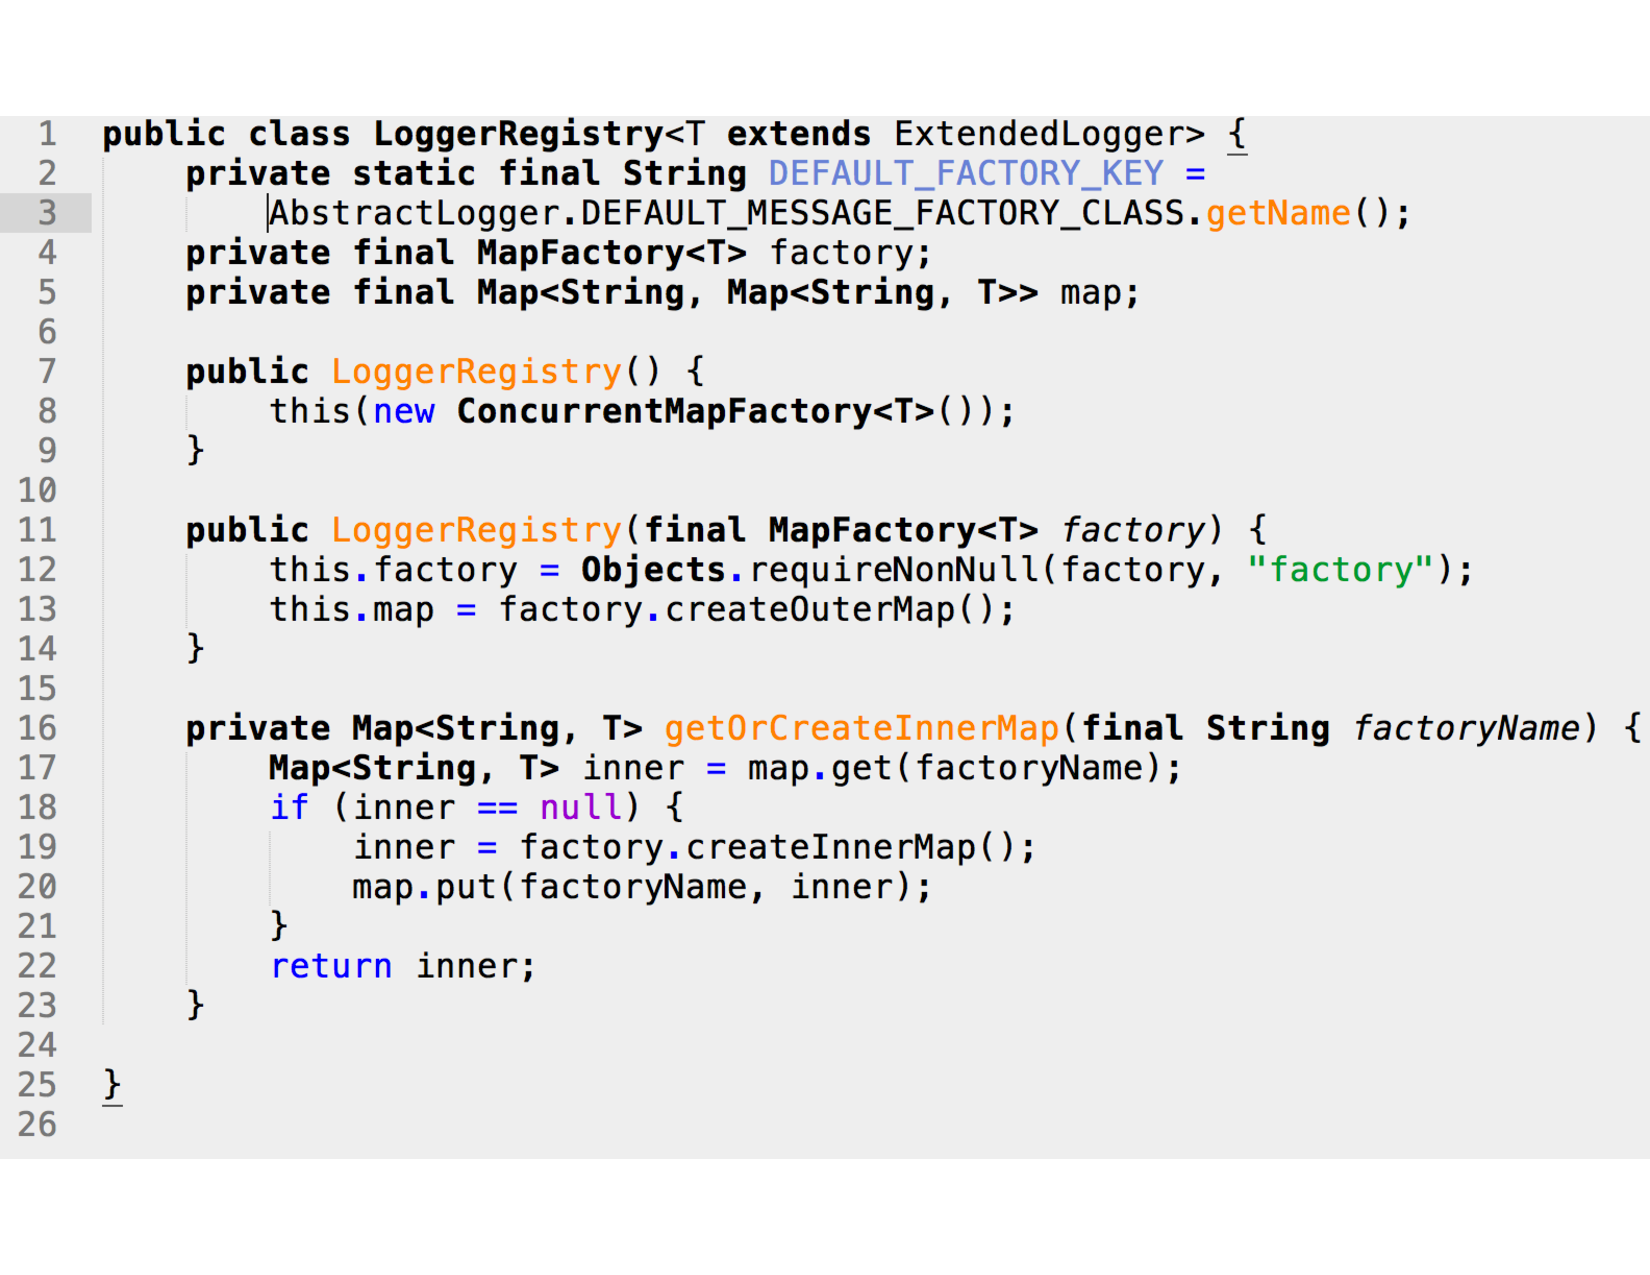
\includegraphics[width=\textwidth]{Chapter-2/figs/code-example.pdf}
	\caption{A source code example for writing to a log file.}
	\label{fig:code}
\end{figure}

Consider, for example, the following source code in Figure~\ref{fig:code}. The requirement, or human-oriented concept, at play is ``write to log file''. If a notification was attached to this code, it would be telling the developer something about the code she wrote to ``write to log file''.
There are multiple programming concepts at play, which aligns with the types of notifications the developer could get. 
In the process of writing this code, the developer could get a notification regarding any number of programming concepts (buffered streams, exception handling); for example, tools like FindBugs, Sonar, and IntelliJ's built-in static analyzers notify developers when they have opened a stream (\texttt{BufferedWriter} in the above example) and there is a possibility the stream that is writing to the file is not closed.
A developer may also get a notification regarding exception handling. Here, the developer has written code to catch an \texttt{IOException} if it occurs. However, if she did not implement code to deal with the potential for an \texttt{IOException} she would get a compiler notification communicating the need to do so.


% TODO later, should note that focusing on programming oriented concepts because those generalize and are foundational to developing the abstractions that are human oriented concepts (biggerstaff)


% RELATED WORK

Research related to mine falls under the following categories: evaluating and improving tool usability, improving notification understanding and resolution, predictive user models, and developer knowledge representation.

\section{Program Analysis Tool Usability}
% TODO: make sure exhaustive here; check studies on dynamic analysis tools too!

There have been many studies on program analysis tools, many of which focus on
their correctness and functionality~\cite{Ayewah:2008:FindBugs,Bessey:2010:Coverity,dugan2000developing,luk2005pin}.
Unlike existing work, which typically focuses on one type of program analysis tool, my work focuses on developers' perception on 
using different types of program analysis tools, what may have caused their perceptions, and how we can build on or improve their perceptions. 
Perception plays an important role in when considering human and computer interactions~\cite{Dastani:2002:Perception} and
can be influenced by a number of things, such as the subjective preferences of
the user.

% TODO: flesh this out
Pettit and colleagues studied the effect of enhanced compiler messages for students\cite{pettit2017enhanced}.
They found no significant improvement, based on likelihood of successive compiler errors, compiler error occurrence, and progress students make towards successful project completion.
Their enhancements were designed without rationale, only focusing on students. Also, the information the was same no matter how much students already knew. Enhancements were made based somewhat on assumed knowledge; the adaptations I am proposing would be based on actual knowledge.
I also assessed other types of enhancements, such as inclusion of examples and links to external information.

Hamou-Lhadj and Lethbridge surveyed trace exploration tools to determine how these tools 
can be used by developers and potential improvements to trace exporation tools~\cite{hamou2004survey}. 
Based on their evaluation of the tools, they found that areas 
for improvement for these type of tools include visibility during trace removal and automated suggestions.
Pacione and colleagues conducted a case study on five dynamic visualization tools that perform either static or dynamic code analysis and observed the output provided~\cite{pacione2003comparative}. Pertaining to usability, they found that level of abstraction can make a difference when explaining large scale problems.

Storey and colleagues ran user experiments with 12 developers on two approaches for presenting software structure in a reverse engineering system~\cite{storey1997rigi}. They found that certain interfaces are better for low-level tasks and that users prefer reverse engineering tools with consolidated interfaces, rather than multiple windows.
Bennett and colleagues conducted interviews and user experiments to evaluate the usability and potential improvements of their sequence diagram creation and exploration tool~\cite{bennett2008survey}. Sequence diagram tools create sequence diagrams using static analysis, dynamic analysis, or both.
Much of the feedback developers provided suggested search and selection highlighting are both useful feature for sequence diagram tools, though there are improvements that can be made to existing implementations.


Ayewah and Pugh conducted a study where they claimed that static analysis tools
should help engineers find bugs as early as possible in the development cycle,
when they are cheap to fix~\cite{Ayewah:2008:FBSurvey}. They interviewed 12
FindBugs users by phone and conducted a controlled study with 12 students to see
how they use FindBugs and handle defects that are labeled ``not a bug''. 
Ayewah and Pugh also conducted a study on using checklists for triaging bug
reports~\cite{Ayewah:2009:Checklists}. In their study, they asked students to
complete a checklist based off the warnings produced by FindBugs in order to
identify warnings that are most important to the users. The checklist gave
different scales used to measure warning severity and relevance and was used
for 13 different warnings.
%Their work is similar to ours in that they are interested in how developers use static
%analysis tools. Our work builds on this work by recruiting various
%tool users for interactive, participatory interviews.

Khoo et al. examined and focused on the interface of static analysis tools and
how the interface could be improved~\cite{Khoo:2008:PathProjection}. They
developed a user interface toolkit called \emph{Path Projection} that uses
program visualizations to help developers walk through the error reports
produced by static analysis tools.
\emph{Path Projection} was designed to improve and simplify the process of
triaging bug reports, or labeling bugs as a false or true positives, by
utilizing checklists to systematically label bugs. This research is similar to my
work in that they look at improving the static analysis tool user experience.
My research builds on this work by investigating not only improving the user
experience, but also finding out why these improvements need to be made from the
developers who use them.

% Although
% both of these studies look at improving static analysis tools or its interface
% to increase and improve the usage of static analysis tools, they still do not
% investigate whether these interface changes are what developers really want or,
% if they are, why. Our study builds on these studies by investigating not only
% improving the user experience, but also finding out why these improvements need
% to be made from the developers who use them in order to better understand how to
% make improvements without focusing on specific functionalities or design ideas.

Heckman and Williams conducted research in an attempt to develop a benchmark,
FAULTBENCH, that would help developers compare and evaluate static analysis
alert prioritization and classification techniques~\cite{Heckman:2008:Faultbench}. 
The overall goal of their research was to make using static analysis tools easier and more useful to developers.
My work is related in that I am also looking for ways to improve the current state of tools for developers. 
Layman et al. recruited 18 participants to investigate factors that developers may consider when deciding whether to
address a defect when notified of it~\cite{Layman:2007:FaultFix}. This study
is related to my work in that they are also interested in learning more about how developers use tools available to them 
and how usage can be made easier.  My work builds on these works by focusing on various
aspects of using program analysis tools, including how users interact with the
tools.

\section{Aiding Notification Resolution}

Existing research has focused on easing the process of understanding and resolving notifications~\cite{Hartmann:2010:Suggestions,Mucslu:2012:Speculative,pham2015automatically,fritz2014developers} from one particular tool.
Rather than studying program analysis tools separately, we believe it is more fruitful to understand the challenges developers encounter across multiple program analysis tools.
As we describe in this section,
existing studies that examine multiple tools typically either focus on tools of the same type (i.e. multiple compilers) 
or helping developers make informed choices among tools. 
Our work is related in that our findings can be used to improve the design of tools to better support developers.
Our work differs in that we investigate different types of tools to identify general challenges developers encounter when interpreting notifications across tools. 

Much of the research on improving developers' ability to interpret tool notifications has focused on compiler notifications~\cite{Hartmann:2010:Suggestions,Traver:2010:Messages,barik14}. 
Hartmann and colleagues developed a social recommender system, \textsc{HelpMeOut}, to better assist novices with understanding and resolving compiler notifications~\cite{Hartmann:2010:Suggestions}. They found their tool provides useful fixes about half of the time. Traver investigated why developers have difficulty with compiler notifications and ways to improve compiler notification design~\cite{Traver:2010:Messages}. Based on his findings, Traver developed compiler notification design principles, which includes using consistent messages and including more visual aids.

Nienaltowski and colleagues studied novice developers' ability to identify errors in their programs and how we can better support that process~\cite{Nienaltowski:2008:Compiler}.
Rigby and Thompson studied novices' use of Eclipse and Gild, a customized version of Eclipse featuring ``novice-friendly'' compiler notifications~\cite{Rigby:2005:Novice}.
Mu\c{s}lu and colleagues developed \textsc{Quick Fix Scout}, an extension to Eclipse Quick Fix, to ease the process of determining an
optimal fix~\cite{Mucslu:2012:Speculative}. They found programmers could more quickly assess and apply quick fixes when able to easily reason about fix trade-offs.
Following up on work with \textsc{Quick Fix Scout}, Mu\c{s}lu and colleagues explored the possibility of improving IDE recommendations, and the ability for developers to determine the best fix for their code, by considering the whole code base rather the local context of the notification~\cite{mucslu2012improving}.
Barik and colleagues studied how developers reason about compiler notifications to improve tool support for understanding and resolving tool notifications~\cite{barik14}.
Compiler notifications are not the only type of notifications a developer might encounter, further supporting the need for cross-tool investigations.
Studying tool notifications across tools, as we have, increases the likelihood our findings can generalize to a variety of tools.

Cross-tool studies that do exist focus on helping developers decide what tools to use rather than tool improvement.
Mettrey evaluated five expert systems tools on factors such as performance, to aide developers in selecting one for their projects~\cite{mettrey1991comparative}.
Wagner and colleagues compared two analysis tools that detect defects to evaluate their efficiency~\cite{wagner2008evaluation}.
Other tool evaluations have had the same goal~\cite{roy2009comparison,zheng2006value}.

Though to our knowledge there are no studies that explore the applicability of communication theory to tool use, there are studies that explore the applicability of other theories to tool use~\cite{barik14,xiao2014social,riemenschneider2001explaining}.  
One is our prior work on how developers visualize compiler messages; we found that self-explanation theory can be used to explain how developers work through compiler error messages~\cite{barik14}. 
In other prior work, we used Diffusion of Innovation theory to explore factors that influence 
security tool adoption~\cite{xiao2014social}. 
Similarly, Rienmenschneider and Hardgrave explored why tools do not get used using the Technology Acceptance Model, based largely on the Theory of Reasoned Action~\cite{riemenschneider2001explaining}.
Lawrance and colleagues used information foraging theory to propose a theory of information foraging for how programmers navigate code when debugging~\cite{lawrance2013programmers}. 
In contrast, we apply communication theory to understand the challenges 
developers encounter when interpreting tool notifications.

\section{Predictive User Models}
Existing research has explored the idea of creating and using predictive user models both in the design of intelligent tutoring systems (ITS) and adaptive user interfaces (AUI). Research also exists that uses code as a proxy for knowledge~\cite{fritz2010degree}. While related, this research proposes models that predict knowledge of source code; my research proposes models that predict knowledge of programming concepts for adapting tool notifications.

Both ITS and AUI use models of user knowledge to adapt to their users, based on the user's experiences~\cite{murray1999authoring}.
ITS pose questions to students to model knowledge of concepts and adapt lesson plans. In contrast, I used source code history to model knowledge for adaption of tool notifications.
Amershi and Conati explored using machine learning rather than knowledge-based user models to deal with the drawback of using knowledge-based user models, as most ITS do~\cite{amershi2007unsupervised}. 
Stamper and Barnes proposed a method for using student data, such as the code they write, to improve ITS with adaptive hints for programming mistakes~\cite{stamper2009unsupervised}.
Similarly, my research explores using source code and machine learning to predict user knowledge but for adaptive tool notifications.

There are a variety of AUI used in different Human-Computer Interaction contexts, many of which use task or domain models~\cite{schlungbaum1996model}. Most relevant to our models in the context of AUIs are works that build and apply user models, such as FUSE, which creates user models based on static and dynamic properties of the user to assist with user interface development~\cite{lonczewski1996fuse}. Most relevant to our research are the models proposed by Zou and colleagues for adaptive menus in Eclipse~\cite{zou2008adapting}.
This AUI's models are built based on how often developers use menu items to remove menu items that are used infrequently; we built models based on the concept-specific code a developer writes to adapt notifications to their experience.


Using source code to represent knowledge relates closely to the degree-of-knowledge models proposed by Fritz and colleagues to determine how familiar a developer is with a particular portion of a codebase~\cite{fritz2010degree}. Their models predict how much a developer might know about a given piece of source code in a codebase based on how often they have visited or edited that part of the code.
Other tools exist that make use of developer source code to make predictions without models. Most relevant is Stylos and colleagues' tool Jadeite which determines API usage examples to provide to a developer based on code other developers have written~\cite{stylos2009improving}.
Along the same lines, Perscheid and colleagues explored the notion that expertise is a good metric for determining who would understand a fault or failure when testing best in a code base~\cite{perscheid2012test}.

Other research has explored how user actions can be used to represent knowledge, mostly in the context of games and learning. Eagle and colleagues conducted research to explore the relationship between the interactions students make in games and understanding science concepts embedded in those games~\cite{eagle2015measuring}. Hicks and colleagues developed an approach to modeling student interactions when using programming tutors and educational games, like BOTS, for predicting the best hints to provide when they are having trouble~\cite{hicks2014building}.
%	In contrast, we predict how much a developer might know about a given concept based on the code she has written.


% McKeithen and colleagues~\cite{mckeithen1981knowledge} - homogeneity within groups (novice, intermediate, expert) but different strategies based on skill level; experts and intermediates similar to each other strategy wise (support decision to eval two instead of three and to put intermediate scores in expert bucket for adaptation purposes)

% TODO other examples RW (add above also):
% Hartmann and colleagues Hartmann:2010:Suggestions - suggest solutions applied by other developers in the past
% Amintabar and colleagues amintabar2015exceptiontracer - help resolve exceptions by adapting relevant solutions from SourceForge and StackOverflow to the context of the exception
% Ponzanelli and colleagues ponzanelli2013seahawk - Eclipse plugin to help developers from within their IDE using StackOverflow using active context




\chapter{Why Don't Developers Use Tools?}
\label{chap:why}

% TODO static analysis --> program analysis ??

Despite the benefits of using static analysis tools to find bugs, consistent
usage of these tools is not very frequent~\cite{Ayewah:2008:FindBugs, ge2012reconciling}. 
There have been studies to investigate ways of improving static analysis tools.
However, none look at what the tools do or can do for a developer, what features
developers use, what could be improved \emph{and}
why~\cite{Bessey:2010:Coverity, Khoo:2008:PathProjection}. The study outlined in this chapter provided an improved understanding 
of why software developers are not using static analysis tools and how
current tools could be improved to increase usage based on developer feedback.
To answer the question \emph{why do developers not use program analysis tools}, I conducted interactive interviews with 20 professional developers to better understand why they do not use static analysis tools, one common type of program analysis tool, to find bugs when writing code~\cite{johnson2013don}.
For this study, I focused on static analysis tools used to finds bugs.
This includes tools like FindBugs, Lint~\cite{Johnson:1978:Lint} ,
IntelliJ~\cite{IntelliJIDEA} (which includes built-in static analyzers), and
PMD~\cite{PMD}. FindBugs will be referenced the most as it is the tool I chose
to use during the interviews.

\section{Exploring Developer Tool Use}

\begin{table}[]
\centering
\caption{Descriptive statistics reported by participants.}
\label{table:demographics}
\rowcolors{2}{gray!25}{white}
\begin{tabular}{llll}
\toprule
\rowcolor{gray!50}
\textbf{Participant} & \textbf{Open Source Tools}                                                                                      & \textbf{Closed Source Tools}              & \textbf{Local} \\
\midrule
Abby                 & FindBugs                                                                                                        & IntelliJ                                  & Yes            \\
Adam                 & CheckStyle, FindBugs, PMD                                                                                       & IntelliJ                                  & Yes            \\
Andy                 & FindBugs, Lint                                                                                                  & Jtest                                     & Yes            \\
Chris                & CheckStyle, FindBugs, Lint                                                                                      & Coverity                                  & Yes            \\
Cody                 & Dehydra                                                                                                         & -                                         & Yes            \\
Frank                & -                                                                                                               & -                                         & Yes            \\
Gordon               & Lint, CheckStyle, FindBugs                                                                                      & -                                         & Yes            \\
Jake                 & FindBugs, Lint                                                                                                  & FlexLint, Klocwork Insight, Visual Studio & Yes            \\
James                & CheckStyle, FindBugs, Lint                                                                                      & Visual Studio                             & Yes            \\
Jason                & FindBugs, Lint                                                                                                  & -                                         & Yes            \\
John                 & \begin{tabular}[c]{@{}l@{}}CheckStyle, Copy/Paste Detector(CPD), \\ FindBugs, Lint, PMD \& CodePro\end{tabular} & -                                         & Yes            \\
Jordan               & CheckStyle, FindBugs, PMD                                                                                       & JTest                                     & Yes            \\
Josh                 & FindBugs, Lint                                                                                                  & Coverity                                  & No             \\
Lee                  & CheckStyle, FindBugs, Lint                                                                                      & Visual Studio                             & Yes            \\
Matt                 & Lint                                                                                                            & FlexLint, PyCharm                         & Yes            \\
Phil                 & -                                                                                                               & -                                         & Yes            \\
Ray                  & CheckStyle, FindBugs                                                                                            & -                                         & Yes            \\
Ryan                 & FindBugs, Ling                                                                                                  & Coverity                                  & Yes            \\
Steve                & CheckStyle, FindBugs, Lint, CPD                                                                                 & IntelliJ                                  & Yes            \\
Tony                 & \begin{tabular}[c]{@{}l@{}}CheckStyle,  FindBugs, Lint, PMD,\\ CPD, cpplint, Splint\end{tabular}                & Coverity                                  &               Yes \\
\bottomrule
\end{tabular}
\end{table}

For this study, I conducted interviews with software developers. Each
semi-structured interview lasted approximately 40-60 minutes and, with the
participant's consent, was recorded. By conducting ``semi-structured''
interviews, I aimed to achieve the flexibility needed to get as much detailed
information as possible~\cite{Hove:2005:Interview}. I prepared a script of
questions for the interview, but would add or omit questions on the fly
depending on how detailed a participant was in their responses.
We created and modified the script as we conducted trial interviews; any changes
made to the script was based on the responses we got from our 4 trial
participants~\cite{Johnson:2012:PreFFSAT}.


Upon completion, I manually transcribed each session. I
performed qualitative analysis \footnote{All study materials including interview
scripts and coding categories are available at
\url{http://www4.ncsu.edu/~bijohnso/ffsat.html}} on the transcripts by
``coding'' the transcriptions. This process is discussed in detail in
Section~\ref{subsec:coding}.

\subsection{Participants}
\label{subsec:participants}

I conducted this study with a group of 20 participants. Although this seems
like a small sample, I followed a similar methodology to that of Layman et.
al.'s study that only had 18 participants~\cite{Layman:2007:FaultFix}.
I recruited participants using an electronic recruitment flyer that was sent
out to industry contacts to then be sent to developers within their company.
Sixteen participants were, at the time, professional developers at a large company and 4
were graduate students at North Carolina State University with previous industry
experience. Participants' years of development experience ranged from 3 to 25
years. We did not explicitly ask participants about their experience building
static analysis tools, however, based on conversations approximately 2
participants had tool building experience. We interviewed two participants
remotely, one by phone and one by video chat, due to location differences. Each
participant filled out a short questionnaire used to collect demographic
information prior to their interview.

Table~\ref{table:demographics} shows the statistics and background information
gathered from the questionnaire and interviews. The first column lists the
participants' pseudonyms, given for confidentiality purposes. The second and
third columns show the open-source tools and closed-source tools that they have
used to find bugs. If a space has a ``-'', it indicates no response from the
participant.  


\subsection{Research Questions}
\label{subsec:rq}
For this study, I answered the following research questions:
\begin{itemize}
\item [RQ\textsubscript{1}]: What reasons do developers have for using
or not using static analysis tools to find bugs?
\item [RQ\textsubscript{2}]: How well do current static analysis tools
fit into the workflows of developers? We define a workflow as the steps a
developer takes when writing, inspecting and modifying their code.
\item [RQ\textsubscript{3}]: What improvements do developers want
to see being made to static analysis tools?
\end{itemize}

I asked these questions because answers to these questions can give toolsmiths
and researchers areas for future work and improvement in the area of static
analysis tool usability. Research has shown that the way a tool interrupts a developer's
workflow is important therefore I also wanted to specifically investigate this
aspect of tool usage~\cite{Robertson:2004:Interruption, Gluck:2007:Attentional}.
The interviews focused on developers' experiences with finding defects using
static analysis tools. Learning developers' relevant experiences and observing
how they use static analysis tools to find bugs may shed some light on why these
tools are underused. I organized the interviews into into three main
parts: Questions and Short Responses (Section~\ref{subsec:part1}), Interactive
Interview (Section~\ref{subsec:part2}), and Participatory Design
(Section~\ref{subsec:part3}).


\subsection{Part I: Questions and Short Responses}
\label{subsec:part1}
During part 1, Question and Short Response, I asked developers questions
related to their general usage, understanding, and opinion of static analysis
tools in order to answer~\hyperlink{RQ1}{RQ1}.

Some of the questions I asked include:
\begin{itemize}
\item Can you tell me about your first experience with a static analysis tool?
\item Can you remember anything that stood out about this experience as easy or difficult?
\item Have you ever used a static analysis tool in a team setting? Was it beneficial and why?
\item Have you ever consciously avoided using a static analysis tool? Why or why not?
\item What in your opinion are the critical characteristics of a good static analysis tool?
\end{itemize}

\subsection{Part II: Interactive Interview}
\label{subsec:part2}
The second part is what I called the ``interactive interview''. The goal behind the
interactive interview is to be able to observe developers actually using a
static analysis tool. This allowed for the gathering of more detailed information as to how
developers are using their tools. I used the information obtained during
this portion to address~\hyperlink{RQ2}{RQ2}. I asked participants to
explain what they are doing out loud~\cite{Lewis:1982:ThinkAloudProtocol} so I
could get a better understanding of their workflow and thought process. Practice
interviews before this study revealed that using the interactive interview
portion produced more detailed information regarding when and how developers use
their static analysis tools~\cite{Johnson:2012:PreFFSAT}.

Some of the questions asked during this portion include:
\begin{itemize}
\item Now that you have run your tool and gotten your feedback, what is your next move(s)?
\item Do you configure the settings of your tool from default? If so, how?
\item Does this static analysis tool aid in assessing what to do about a warning?
\item Do you feel that ``quick fixes'' or code suggestions would be helpful if
they were available?\footnote{Participants were only asked about quick fixes and
code suggestions being useful when they mentioned, either during the Question
and Answer or Interactive Interview, that they either a) find quick fixes
useful, b) felt that the tool should be more helpful or c) did not understand
how to fix the defect we presented them with. }
\end{itemize}

For confidentiality reasons, not all participants could use their own
workstation for this part of the interview. For those who could not, I provided
6 open source projects in Java, such as log4j~\cite{log4j} and Ant~\cite{ANT},
and asked each participant to run FindBugs on one of them.  I chose FindBugs
because it is one of the most popular and mature open source static analysis tools for
Eclipse. Due to technical difficulties, the remote interviews could not fully experience the ``interactive'' portion. 
Each remote participant was given a scenario of static analysis tool usage and asked to, first, explain their thought process in
walking through that particular scenario. I then asked the same questions as I would have asked if they had been local.


\subsection{Part III: Participatory Design}
\label{subsec:part3}

The last part of the interview allowed participants to make
design suggestions for improving static analysis tools. I utilized a concept
called \textit{participatory design}~\cite{Spinuzzi:2005:Participatory}, which involves
getting stakeholders (in this case, the participants) involved in the design
process by allowing them to show what they want instead of saying it. In order
to promote creativity, each participant was given a blank sheet of paper and
asked to sketch what they wanted their tool to look like and describe how it should
work~\cite{Johnson:2012:PreFFSAT}. I did not require participants to draw
something, but 6 of them did. The rest of the participants gave verbal
descriptions of tool features they desired.


\subsection{Coding Interview Responses}
\label{subsec:coding}
After completing the interviews, I manually transcribed each interview.
Then, I \textit{coded} the transcriptions. Coding
is a process that is meant to make referencing transcriptions quicker and
easier~\cite{Gordon:1998:Coding}. I used Gordon's basic steps to code the 
interview transcripts and used the codes to help organize the Results
(Section~\ref{sec:barriers}). According to Gordon's steps, before coding an interview, ``coding
categories'' need to be defined. These should be general enough for relevant
information to be grouped together but detailed enough that a concrete example
only falls under one category. Because of this, it is possible to have
``emergent'' categories that may need to be defined after reading the
transcriptions. I developed and used the following coding categories:

\begin{itemize}
    \item \emph{Tool Output}: anything related to the output produced by
the tool (for example, false positives).
    \item \emph{Supporting Teamwork}: anything about using static analysis tools in a team or collaborative setting
    \item \emph{User Input and Customizability}: points made about the customizability of the static analysis tools (for example, modifying rule sets)
    \item \emph{Result Understandability}:  anything said about the ability or inability to understand or interpret the results produced by a static analysis tool
    \item \emph{Workflows}: anything related to the steps a developer takes when writing, inspecting and modifying their software (for example, tool integration)
    \item \emph{Tool Design}: the proposed tool design ideas from our participants.
\end{itemize}

\noindent Examples of each of these categories from the transcriptions are as follows:
\begin{description}
\item[Tool Output] \hfill \\
    Jason: \emph{``\ldots like I mentioned with FlexLint it gives you so many warnings and sifting through them is so, arduous that whenever I just
look at it I'm like ehhh forget this.''}

\item[User Input/Customizability] \hfill \\ 
	Andy: \emph{``\ldots it's like is this
list prioritized by you know what's important to me? No. You know? And there
may be a default listing that should be prioritized because like this one's
inefficient.''}
\item[Supporting Teamwork] \hfill \\
	John: \emph{``The only reason I like the batch
results is to communicate, broadcast to the team a sense of progress or lack of
progress.''}
\item[Result Understandability] \hfill \\ 
	Matt: \emph{so now I wanna know why raising a string
exception is bad. Like what should I be doing instead? Since it thinks it's a
problem. And so none of these really help me.}
\item[Workflows] \hfill \\
	Mike: \emph{``Clang is my favorite. It's built into the compiler. You don't
have to invoke anything special.''}
\item[Tool Design] \hfill \\
	Chris: \emph{``I don't mind the idea of the actual source code itself having
some plasticity \ldots let's say the fourth line there was some error
here\ldots having the 5th line drop down and having the content expand with maybe all
sorts of annotations about my code.''}
\end{description}

The next step in Gordon's methodology is to assign ``category symbols'' to each
category for easier indexing and processing of information. Gordon then suggests
finding and classifying the relevant information in the transcriptions using the
category symbols. In my set of codes, each coding category had its own color as a
``symbol''; if a portion of a participant's transcription fell into one of the
categories, the text would be highlighted the same color as its respective
category. A participant's coded interview could contain multiple categories or
even multiple data items for one category. To ensure consistency, only I was
responsible for coming up with the coding categories and ``symbols'' and going
through the transcriptions to apply them. The last step is to check the
reliability of the codes. For this study, once the coding was complete, I passed the documents over to other contributors to look over. 
If there were any discrepancies we discussed and resolved them as a group. This includes items
that could fall into more than one category; in this situation, either a new,
more specific, category or a ``sub-category'' was created for the item. The
purpose of the categories are to organize the data in a relevant and useful
manner; they are not meant to directly correlate with the research questions. 
The next section discusses findings from this study.

\section{Barriers to Tool Use}
\label{sec:barriers}

In this section, I will discuss the results obtained from the interviews. I answered my
research questions by linking the questions to coding categories and interview
parts.

Based on the data collected, the following was true:
\begin{itemize}
    \item My first research question (\hyperlink{RQ1}{RQ1})
was answered by observing the results categorized under ``Tool Output,'' ``Supporting Teamwork,'' ``User Input and
Customizability,'' ``Result Understandability'' and ``Developer Workflows''; the
information collected in these categories could be reasons why developers are or
are not using static analysis tools.
    \item My second research question (\hyperlink{RQ2}{RQ2}) was answered by
observing the results categorized under ``Developer Workflows.''
    \item My third research question (\hyperlink{RQ3}{RQ3}) was answered by
observing the results categorized under ``Tool Design''; most of
these results are from the Participatory Design portion.
\end{itemize}

In each category, I expected there to be negative and positive remarks about
current tools, both of which are equally important in answering my research
questions; anything positive could be a reason for use while anything negative
could be a reason to discontinue use.
For each coding category, I separated the relevant statements into positive
statements and negative statements; if something good is said about a static
analysis tool it is considered a \emph{positive} comment and vice versa for a
\emph{negative} comment. In Figure~\ref{fig:results}, we can see that the
majority of participants have had problems with tool output, customizability
and workflow integration, and all but one of participant has had problems
with understanding the results of tool analyses. Tool design is not included because this category
was defined to capture the developers' ideas for improving static analysis
tools. Their reasons for wanting the features are captured in the other
categories.

\begin{figure*}
\centering
\includegraphics[scale=0.65,clip]{Chapter-3/figs/results.eps}
\caption{The number of participants in each category expressing the good and the bad about static analysis tools they have used.}
\label{fig:results}
\end{figure*}

\subsection{RQ1: Reasons for Use and Underuse}
\label{subsec:rq1}

The interviews revealed that there are a variety of reasons developers may have
for choosing to use a static analysis tool to find bugs in their code. One of
the obvious reasons is because too much time and effort is involved in manually
searching for bugs. Five out of 20 participants felt that because static
analysis tools can automatically find bugs, they are worth using. During his
interactive interview, Jason told us ``\emph{anything that will automate a
mundane task is great.}'' In other words, one reason for using static analysis
tools is that they automate the process of finding bugs.

Another reason developers might use a static analysis tool is if it is already
available in the development environment and ready to be used. For 3 participants, this was the case. 
Development environments such as IntelliJ and
PyCharm come with built-in static analyzers, which requires little extra effort
on the developer's part. Two participants, Matt and Adam, used PyCharm and
IntelliJ regularly and liked the fact that static analysis was already integrated.
For 7 participants, a good reason to use static analysis tools is to
support team development efforts. According to Josh and Andy, static analysis
tools do this by raising awareness of the potential problems, or ``dumb
mistakes,'' in the code earlier in the development process. For Cody and Ray,
static analysis tools are useful for communicating and enforcing coding
standards and styles on development teams. Some developers enjoy using the
static analysis tools they use to find bugs because of the level of
customizability. Three participants fit into this category. According to
James, the customizability of a tool can play a large part in the volume and
quality of output developers get.
% Cody likes using Dehydra~\cite{Dehydra} because it is easy to write new rules
% as well as modify the existing ones. <-- removed because not completely
% necessary, doesn't hurt anything when removed and for the sake of space

% ~\BIJ{I can put more here; I was trying to group them to show that there were
% things people agreed on but there were a few other things I could add}
Although some participants could find reasons to use static analysis
tools to find bugs, most of our participants brought up conflicting concerns
that could make the decision to adopt and regularly use static analysis tools less
obvious.

\textbf{Tool Ouput.} 
Tool output was a popular discussion topic. Out of the 20 developers I
interviewed, 14 expressed the negative impacts of poorly presented
output. Static analysis tools are known to produce false positives and these
false positives can ``outweigh'' the true positives in
volume~\cite{Shen:2011:EFindBugs}. Another known fact is that, especially with
larger projects, the number of warnings produced by a tool can be high,
sometimes in the thousands~\cite{Ayewah:2010:GFF}. Some participants
felt, however, that false positives and large volumes of warnings would be less
burdensome if the way the output is presented was more user-friendly and
intuitive. Cody, who likes using Dehydra, finds himself frustrated at times
because the results are dumped onto his screen with no distinct structure
causing him to spend a lot of time trying to figure out what needs to be done.
Jason wishes that his tool's output would be a ``slice'' that shows what the
problem is and what else could be affected in order to more quickly assess what
is or is not important. This ``slice'' should be taken from the entire project,
using call hierarchies, to show which parts are affected by each defect. During
his interactive interview he commented on a previous experience with FindBugs.
He had a large list of warnings to scroll through but without there being any
context to the problems it just seemed like ``a bunch of junk to sift through,''
which made him not want to bother using it. It may be worth investigating
how valuable an output like this would be.

\textbf{Collaboration.}
In industry, software development is often a team effort. For 9 participants, lack of or weak support for teamwork or collaboration was one
reason that teams, as well as individual developers, may not adopt or regularly
use static analysis tools.
According to John, although static analysis tools are useful for trying to
enforce coding standards, there is no easy way to share the settings with other
people on the team so it ends up being a cumbersome manual process and causing
confusion when the standards need to be changed. Many participants
mentioned the desire for a way to easily communicate and collaborate when using
their static analysis tool, especially in a team setting.
% For Matt, version control is more helpful when it comes to working and
% communicating on teams.
Although static analysis tools can be beneficial in team settings, current tools
are not collaborative enough for some developers. Newer versions of FindBugs
offer a cloud storage feature that can be used store, share and discuss warning
evaluations~\cite{FindBugsCloud}. Although a feature like this does make it
easier to communicate and share warning evaluations between developers, to add a
comment to a bug or current evaluation a web browser is needed. This takes the developer
out of context and out of the development environment which could demotivate
some individuals from checking them when they should.
% It may be worth investigating how to make static analysis tools more
% collaborative to support the sharing of information related to code analysis,
% such as coding standards or rule sets.

\textbf{Customizability.}
For 17 participants, customizability was important however many tools are
not trivial to configure and do not accommodate the customizations that
developers want. False positives and large volumes of warnings are well-known
downsides to using static analysis tool to find bugs. However, Frank told us he
believes that the way a tool is configured plays a large part in the output
a developer gets. John stated during his interview that ``\emph{many tools are so hard to
configure, they prevent you from doing anything.}'' Sometimes it is difficult
just to get to the menu where the options for configuring a particular feature
are, which participants Matt and Josh agree with. One participant, Jake,
found himself in an interesting situation during his interactive interview where
he could not figure out how to customize his tool and wound up having to search
the web to locate the tool's preferences. A common problem
expressed by most of the participants is the inability to temporarily ignore or
suppress certain warnings. Although some static analysis tools allow developers
to turn off certain filters, not all developers are comfortable with turning
warnings completely off. Matt, for example, is afraid that he may not remember
to turn it back on. The notion of dismissing or ignoring static analysis
warnings may be too coarse; as Jordan noted, he would prefer if static
analysis tools offered a way of recording his judgement about a given warning. More
sophisticated judgements may include things like ``this warning isn't a problem
now, but may be in the future if the following conditions are met\ldots''.

\textbf{Result Understandability.} 
The main objective when using a tool like FindBugs is to learn what defects are
in the code so that problems can be removed. A developer not being able to
understand what the tool is telling her, according to participants, is a
definite barrier to use. Nineteen out of 20 participants felt that many static
analysis tools do not present their results in a way that gives enough
information for them to assess what the problem is, why it is a problem and what
they should be doing differently. James told us during his interview that
``\emph{it's one thing to give an error message, it's another thing to give a
useful error message.}'' When talking about the Eclipse Python plug-ins, he also
stated, ``\emph{I find that the information they provide is not very useful, so
I tend to ignore them.}'' A few participants felt that it would be helpful to
have links to more details or examples in the error reports.
In some situations more information is needed to understand exactly what the
problem is and why it is a problem; understanding why a defect is a problem can
help the developer better assess whether the error is a false positive and try
to avoid repeating the same problem. Ryan told us during
his interactive interview that a start would be using ``real words,'' or a more
natural language, to explain the problem.

The most frequently mentioned difficulty when using static analysis tools was
lack of or ineffectively implemented quick fixes.
Most participants expressed interest in having their tool provide code
suggestions or quick fixes that assist them when attempting to fix a bug; Abby
proclaimed ``\emph{if you can tell me it's an error, you should be able to tell
me how to fix it.}'' Jordan strongly agrees; he loves tools that have quick
fixes and hates tools that do not. According to the interviews, these fixes do
not have to be automatic; some prefer that code suggestion previews be used or
possibly using examples to get a better understanding of how to fix the problem.
Some participants expressed interest in but skepticism toward integrating quick
fixes into static analysis tools. For example, during Jordan's interactive
interview, he noted that sometimes when using multiple tools, they may
have conflicting quick fixes or solutions. In Frank's past experiences with
automated code changes, he has had to do manual refactorings because something
was done wrong; because of this, he prefers to use find and replace to make
his own changes. Another participant, Adam, was concerned with knowing whether
the semantics of his code would be preserved after applying a quick fix. Most
static analysis tools, if they offer quick fixes, leave it to the developer to
figure out exactly what has been done after it has been done. Almost all of the participants agreed 
that effectively designed quick fixes can help them to better
understand the problems tools tell them about, leading to a better
sense of productivity for the developer.


\subsection{RQ2: Workflow Integration}
\label{subsec:rq2}

The most common topic during the interviews was
tool and environment integration. Sometimes a developer's process includes
running a static analysis tool, but more often it is not part of a
developer's workflow to stop and run a tool in the middle of working on some
code or a specific task; she usually prefers finding a ``stopping
point'' in her code to run the tool~\cite{Layman:2007:FaultFix}. Analysis of
these interviews revealed that while this is true, there are many different ways
that developers may want their tool to fit into their development workflow. For
example, some developers prefer that the tool run in the background; it
is easier for them to figure out what is wrong if they are in the process of
doing it and do not have to think about invoking the tool.
On the other hand, some developers do not
use IDEs, so if they are to use a static analysis tool, compiler
integration is very important. Nineteen of the 20 developers I interviewed
expressed the importance of workflow integration to them and how these needs have
been or should be met.

For some participants, there are features of static analysis tools they
have used that helped the tool better integrate into their workflow leading to
increased usage of the tool. In fact, John felt that
static analysis tools can be used to help organize a workflow, based on the
results it produces. For example, running a static analysis tool on
some code for the first time can be a good indicator of the kinds of bugs
the tool finds and that may be present; this can give an idea as to how detailed
of an analysis the tool provides, possibly giving a better idea of when it
would be best to run it. Of all the tools Adam has used in the past, he
much preferred to use IntelliJ and its built-in static analysis to find bugs; they
are tightly integrated making it seem more ``real time''. For these
participants, as well as a few others, integration with the development
environment plays a major role in their decision to use or continue using a
static analysis tool. Common standalone static analysis tools like FindBugs and
PMD have the ability to integrate with IDEs like Eclipse and NetBeans which
becomes especially important when using more than one static analysis
tool at a time, as we learned from discussing a past experience of Steve's where
he used 3 different static analysis tools at once. Jordan and
Chris like how FindBugs, PMD and CheckStyle fit into their
development processes; for Jordan, it is an integral part of his workflow. For the
majority of participants, however, current static analysis tools are not
doing enough to effectively integrate into their development process.

One of the biggest demotivational forces on a developer when it comes to using a
static analysis tool to find bugs is when it is what Tony calls a ``disjoint
process.'' Many participants, especially those who do not use IDEs, do
not like when they have to go out of their coding environment to use a tool or
view the results produced by the tool. For example, Frank, Lee, James and Andy
commented on how ``painful'' it was during their interactive interview to have
to switch perspectives in FindBugs to explore the complete
listing of bugs. According to Lee, having to open another perspective to know
what is going on is a guarantee that unmotivated people will not do it. For
Frank, although it is nice that the results are hidden so that you are not
overwhelmed, having to go back and forth and drill down to see the bugs requires
extra effort and is disruptive to his workflow. Other tools participants had
similar complaints about was Coverity and Lint for C/C++ projects. For Ryan and
Tony, the biggest downside to using Coverity is that it is not capable of being
integrated into their coding environment, leading to a lot of clicking back and
forth between their editor and the static analysis tool. Phil does not like
using Lint because of the fact that he has to ``go out of his way'' to do so.

Some participants made it clear, however, that even if the tool is
integrated with their development~\emph{environment}, it is still possible that
the tool does not integrate well into their development~\emph{process}. For
example, Mike does not use IDEs so using a tool that
integrates well with an IDE does not fit well into his development process; he
likes using Clang because it can be tied into his compiler which does not
require a ``development environment''. According to Gordon, one of the key
problems with static analysis tools is that at times they can prevent him from
being productive. One way this can happen is when the tool slows the developer
down by taking a long time to run, which was a common complaint amongst participants in this study. 
From Jason's experience, he believes that ``\emph{if it disrupts
your flow, you're not gonna use it.}'' Jason's statement rang true among other
participants as well, like Steve who had used various tools in his past but did 
not like to use FindBugs because, even though it is IDE integrable, it runs
slow. IntelliJ, which contains built in static analyzers, utilizes~\emph{idle
time} when reporting bugs in an attempt to prevent the problem of interrupting
the developer's workflow but for Matt, it can still be bothersome.
Jason believes that the problem with current static analysis tools is that they
are not capable of running well on larger code bases, leading to a break in his
``development flow'' as he waits for the tool to catch up.

In terms of workflow, participants valued using static analysis both to fix bugs
once they are introduced into the program, but also later in the development
process. From a workflow standpoint, it is valuable to fix potential bugs when
they are entered into a program because the necessary context to understand the
bug is already in the developers' working memory. In contrast, fixing bugs later
is difficult because a developer must recall the context to analyze the
corresponding static analysis warning. This contrast is similar to the
difference between ``floss refactoring'' and ``root canal refactoring,'' where
the former involves restructuring code as it is being worked with and the latter
involves refactoring by finding the ``worst code'' and dealing with that
first~\cite{Murphy-Hill:2008:RefactoringTools}.
Root canal refactoring is a discouraged practice and its analog in static
analysis -- finding the most severe static analysis warnings in a whole codebase
and dealing with those first -- may also be a wasteful practice. Research has
shown that many static analysis warnings in working systems do not actually
manifest as program failures~\cite{Ayewah:2010:GFF}.


\subsection{RQ3: Tool Design}
\label{subsec:rq3}

My main research goal to determine how we can improve static analysis tools for
developers. The best way to do this is to find out how developers want their
tool to be designed. Most of the proposed designs are for warning notification
and manipulation or quick fix display. Participants made some other interesting
proposals which will also be presented.

\textbf{Quick Fix Design.}
Ten participants made a suggestion related to the way in which a quick
fix should be displayed. Most participants wanted to be able to preview
the fix and how it is going to change their code before they apply it. Abby and
Tony recommended splitting the code editor to show a diff of the code, using
highlighting to show what code has changed or been added to their code. On one
side there would be the code now and on the other the code once the fix is
applied. Some felt that you should be able to see the fix before applying it,
but then also manually apply it so that you know the fix is being
applied without introducing any new problems.
One participant, Mike, prefers not to have quick fixes at all because he feels the error messages are enough to
assess what to do about an error.

% TODO talk about/cite FixBugs somewhere??
One interesting quick fix design idea, which came from Ryan during his
interactive interview, was to have what he called a ``\emph{three option dialog
box}'' available when applying a quick fix. This dialog box would pop up upon a
click to fix the bug and there would be three choices: apply the entire fix
(default option), do not apply the fix or step by step apply the solution
allowing the developer to decide which parts of the solution they would like to
keep. Static analysis tools like FindBugs and IntelliJ offer some quick fixes.
However, they do not give a full context preview of the changes that will be
made, leaving it to the developer to manually ensure that the fix was applied
correctly and to their liking.


\textbf{Warning Notification and Manipulation Design.} All 20 participants told us when and how they wanted to be notified of errors in their
code. The theme in this category is ``fast.'' Developers want tools that provide
faster feedback in an efficient way that does not disrupt their workflows. For
some participants, this meant running the tool in the background of the
IDE so that feedback occurs as soon as a problem is detected.
For other participants, this meant running the tool at build time or compile
time.  In this way, the results are presented when the developer is at a predefined ``stopping point."~\cite{Layman:2007:FaultFix}.

Overall, participants found that current static analysis tools are not fast
enough when providing them with feedback; this quickness should be accompanied
with discretion as the developer does not want the tool to break their thought
process.

Participants also thought it would be beneficial to have the ability to
easily make ``judgements'' about defects, such as setting it aside to view
later, save these judgements and share them with other developers. Many participants suggested that static analysis tools should allow developers to
ignore specific defects and move them to their own list for later viewing, a
form of \emph{temporary suppression}. Most tools, if they allow the developer to
ignore specific warnings, only allow the developer to turn off or suppress a bug
category for particular line of code using a comment-like annotation, which
Gordon told us makes the code ``smell''. Developers would like to have the
option to ignore each individual defect in case they either do not want to fix
it and do not want to be bothered by it again or do not want to be bothered with
it at that particular time but would like to come back to it later.

\textbf{Other Design Ideas.} Participants also came up with creative design
ideas. One participant, Chris, suggested giving the editor ``plasticity''. When
he is given a warning and would like to get more information, the tool should
move the code surrounding the warning to embed this information into the editor.
A couple of participants thought it would be useful to have visual output,
possibly a pie-style diagram of the project and the bugs in it, instead of
standard list and tree outputs to make it easier to go back and forth between
warnings and code. During Frank's participatory design session, he suggested a
potential solution; a parts-to-a-whole corpus view of the project as a
~\emph{``heat map''}. The heat map would use colors to show where the errors are
and how severe the problems are. It would start with an overall ``view'' of the
project and as you drill down you can see the condition at each level to see
where the most attention is needed. This is similar to the concept behind Khoo's
toolkit ~\emph{Path Projection} in that the toolkit is meant to visualize output
that is usually, if not always, textual and difficult to
understand~\cite{Khoo:2008:PathProjection}.


An interesting suggestion made by a couple of participants was to represent
the severity of the defects using gradients of one color instead of multiple
different colors; the darker the color the more important or urgent the bug is.
Figure~\ref{fig:participatory} depicts a drawing one participant, Matt,
drew during his participatory design; he labeled the side of the editor
``gradient'' (A) where he would like to see his severity representation. In the
top right corner, Matt also lists the colors that his current tool uses (B); for
example, ``R'' means red. The idea behind this is not new; other studies have
focused their attention on using colors for error
representation~\cite{Oberg:1992:Gradients, Murphy-Hill:2010:StenchBlossom}.
% Oberg and Notkin experimented with using graduated colors to notify the user
% of the \emph{age} of a defect; the darker the color the older the bug. This is
% similar to what our participants suggested except they want the color to
% represent how \emph{severe} the defect is. Murphy-Hill and Black propose a
% ``code smell'' detector that uses colors to indicate how obvious the code
% smells are in the code to the developer. If the code smell is one that the
% developer is likely to notice, the indicator is blue; if the code smell is one
% the developer is not likely to notice, the indicator is orange. Gradients
% between blue and orange are used for code smells that may be in between. This
% is also similar to what our participants suggested, however this approach uses
% gradients in between two different colors and the colors are used to represent
% the \emph{obviousness} of code smells.

\begin{figure}
\centering
\includegraphics[scale=0.5,clip]{Chapter-3/figs/participatory.eps}
\caption{One of our participant, Matt's, Participatory Design drawing; (A) shows where Matt wants the gradient colors and (B) shows the way his current tool represents severity.}
\label{fig:participatory}
\end{figure}

\subsection{Threats to Validity}

There exists threats to the validity of this study;
here I categorize each threat as a threat to external,
internal, or construct validity.

\textbf{External.} One limitation to the generalizability of this study is the
sample size. Although I obtained valuable information from the 20 interviews,
due to time constraints (and busy developers) they may not be representative of
the larger population that use static analysis tools. Although we would have
liked more participants, having a large number of interviews to transcribe and
code could lead to less accurate analysis. The study conducted by Layman et
al.~\cite{Layman:2007:FaultFix}, which we discussed earlier as utilizing a
similar methodology, had a participant pool of similar size (18).
Another possible threat is that we only interviewed developers who have used
static analysis tools. In some cases it may be that static analysis tools are
not being used for other reasons, such as lack of awareness. It should also be
noted that some participants had experience building static analysis
tools, giving them somewhat of a biased opinion of the usage of these tools.


\textbf{Internal.} Another threat to the validity of this study is the way in
which I conducted the remote interviews.
I did not thoroughly prepare for what I would do if the technology I wanted
to use did not work or was not available. Therefore, the interactive interview
and participatory design in remote interviews had to be conducted differently
than local interviews. Despite this, there was still value in the results
obtained from the remote participants; they could still give useful insights
from their previous experiences. Only 2 of the interviews fell into this
category, so this helps limit the impact of this threat.

\textbf{Construct.} The objective for using the interactive interview was to get
more accurate information on how developers use their tools. One limitation here
is that some developers were not as familiar with the code or environment they
had to use in the interviews as they would be with their own code in their own
development environment. This could have caused some developers to take
different actions than they would have in their own environment. Ideally
it would have been better to have been able to observe participants working
in their own environment; however, for confidentiality reasons, we could not view participants' proprietary code. 
In an effort to compensate for this threat, the open source projects and tool we chose are well-known, frequently used open
source projects. Another threat to the validity of this work is that I did not
originally consider that I may have said things in the consent form or
session script that would have given unintended ``hints'' to participants
concerning my research expectations. One example of this is my outlining the research goals in the introductions I gave prior to beginning each session.
This could have led to what is called ``hypothesis guessing'' where participants
respond to questions based on what they think the researcher wants to
hear~\cite{Threats}. In retrospect, I helped alleviate this threat in the interviews
by asking participants experience questions.

\section{Next Steps to A Solution}
% this study explored the what (what's causing developers to not frequently use tools). Most common findings = notification understandability. Next study/question that needs to be answered is why developers have difficulty with notifications -- only then can we start to explore ways to mitigate barriers and potentially increase usage/improve opinion of tools.

% interactive quick fixes (help with resolution)
\subsection{Notification Resolution Solutions}

For many developers in the study above, it was important that their tools help them with resolving the defects found in their code.
Current static analysis tools may not give enough information for
developers to assess what to do about the warnings produced and very seldom
offer a fix to what it claims is an issue. If static analysis tools offered
quick fixes, giving a potential solution and applying it to the problem may help
developers assess warnings more quickly and ultimately save time and effort. My
results indicate that FindBugs, for example, would be more useful if it had more
informative messages and offered quick fixes. 

At the same time, quick fixes do not appear to be a universally applicable mechanism to help
developers resolve static analysis warnings because many static analysis
warnings do not have a small set of solutions. For example, FindBugs warns
developers when two method names in the same class differ only by
capitalization; no quick fix for this problem is likely to satisfy a developer.
Instead, interactive quick fixes that enable easy access to refactoring and code
modification tools may be able to semi-automatically help developers resolve
static analysis warnings. Barik and colleagues developed and evaluated an approach for interactively resolving defects based on these findings~\cite{barik2016quick}.

On the negative side, quick fixes could also cause
developers to be hasty in fixing their code, which could potentially lead to
more problems, such as the introduction of new defects~\cite{Mucslu:2012:Speculative}. There are also
challenges related to implementing usable interactive quick fixes. We
have not yet investigated what theses challenges are or how to address them as
they are out of scope for this particular study.

\subsection{Notification Understandability Solutions}
% notification understandability (help with understanding)
According to the findings above, although the point of using tools is to help identify and resolve defects, developers do not find the lack of quick fixes to be as much of a barrier to use as inability to interpret the notifications provided.
The tool, and any available quick fixes, become less useful if the developer does not understand the problem as it is being communicated.
% Based on the data from these interviews, some of the reasons developers do not frequently use static analysis tools are \textbf{Lack of collaborative support}, \textbf{Seemingly unorganized tool output}, \textbf{Poor support for customizations}, and \textbf{Difficult to interpret notifications}. 
Three out of four findings regarding tool use pertain to the notifications tools use and how tools present information to the developer.
Discovering that tool notifications are one of the reasons developers do not use program analysis tools is useful, however, not actionable. The next piece of information needed to make these findings actionable is to discover why developers have difficulty interpreting tool notifications. Only then can we start to explore ways to mitigate these barriers and potentially increase usage of these tools.
By focusing on improving developer ability to interpret tool notifications, I propose we can also improve developer ability to resolve tool notifications. In the next chapter, I discuss a follow-up study that explores why developer have difficulty with tool notifications.

\chapter{Theory of (Mis)communication}
\label{chap:theory}

In the previous chapter, I discussed findings from a study that explored reasons developers have for not using program analysis tools. One reason that almost all developers in that student could agree on is that the output provided by their tools are sometimes difficult to interpret.
Therefore, this chapter presents research that took a deep dive to explore the challenges developers encounter when interpreting tool notifications.

To answer the question \emph{why do developers encounter challenges when interpreting program analysis tool notifications?}, I observed 26 developers with varying backgrounds while they used three different program analysis tools: Eclipse Java compiler, FindBugs, and EclEmma. I presented participants with and asked them to interpret notifications from each of the three tools. 
To identify challenges, I examined tool use through the lens of communication theory~\cite{bowman1987modeling}.
Building on an existing model of (mis)communication~\cite{mustajoki2008modelling}, I identified 12 kinds of challenges developers encounter when interpreting tool notifications.

% TODO should this come first or after challenges listed?
Based on the challenges participants encountered when interpreting tool notifications, I proposed a tool miscommunication theory that can be used to inform the design of program analysis tools.
Experts in qualitative research suggest that rather than presenting a set of disparate findings, qualitative researchers should instead produce an explanatory theory, a ``skeleton or framework that explains why things happen''~\cite{corbin2014basics}. While explicitly putting forward theories is rare in software engineering~\cite{hannay2007systematic}, one example is Lawrance and colleagues' theory of how programmers navigate code during debugging~\cite{lawrance2013programmers}. In the same way that Lawrance and colleagues' build on 
information foraging theory~\cite{pirolli1999information}, my theory builds on communication theory~\cite{bowman1987modeling}.
I summarize my theory as:

\begin{quotation}
	\noindent
	\emph{The challenges developers encounter when interpreting program analysis tool notifications are caused by gaps and mismatches between developer knowledge and how notifications communicate information.}
\end{quotation}

In the following sections, I will discuss the methodology I used to identify developer challenges, the 12 kinds of challenges I identified that informed this theory, and ways in which this theory can be operationalized.

\section{Identifying Challenges}

% TODO this probably becomes an Appendix reference (or maybe separate ones for each thing that can be referenced)
% Research materials are available on-line to aid other researchers in replication and exploration.\footnote{\url{http://www4.ncsu.edu/~bijohnso/esnpat.html}}

%\subsection{Research Question}\label{rq}

In a previous study, I asked developers to recall experiences with static analysis tools and briefly use FindBugs. I found that some developers do not use program analysis tools due to difficulty interpreting the notifications tools use to communicate~\cite{johnson2013don}. 
To find out how tools could better communicate with developers, this study was designed to answer the
question: \noindent\emph{Why do developers encounter challenges when interpreting program analysis tool notifications?} Using Hannay and colleagues' guidelines~\cite{hannay2007systematic}, 
I framed my question as \emph{why} rather than \emph{what} to support the building of a theory that explains the challenges developers encounter.

\begin{figure*} [ht]
\centering
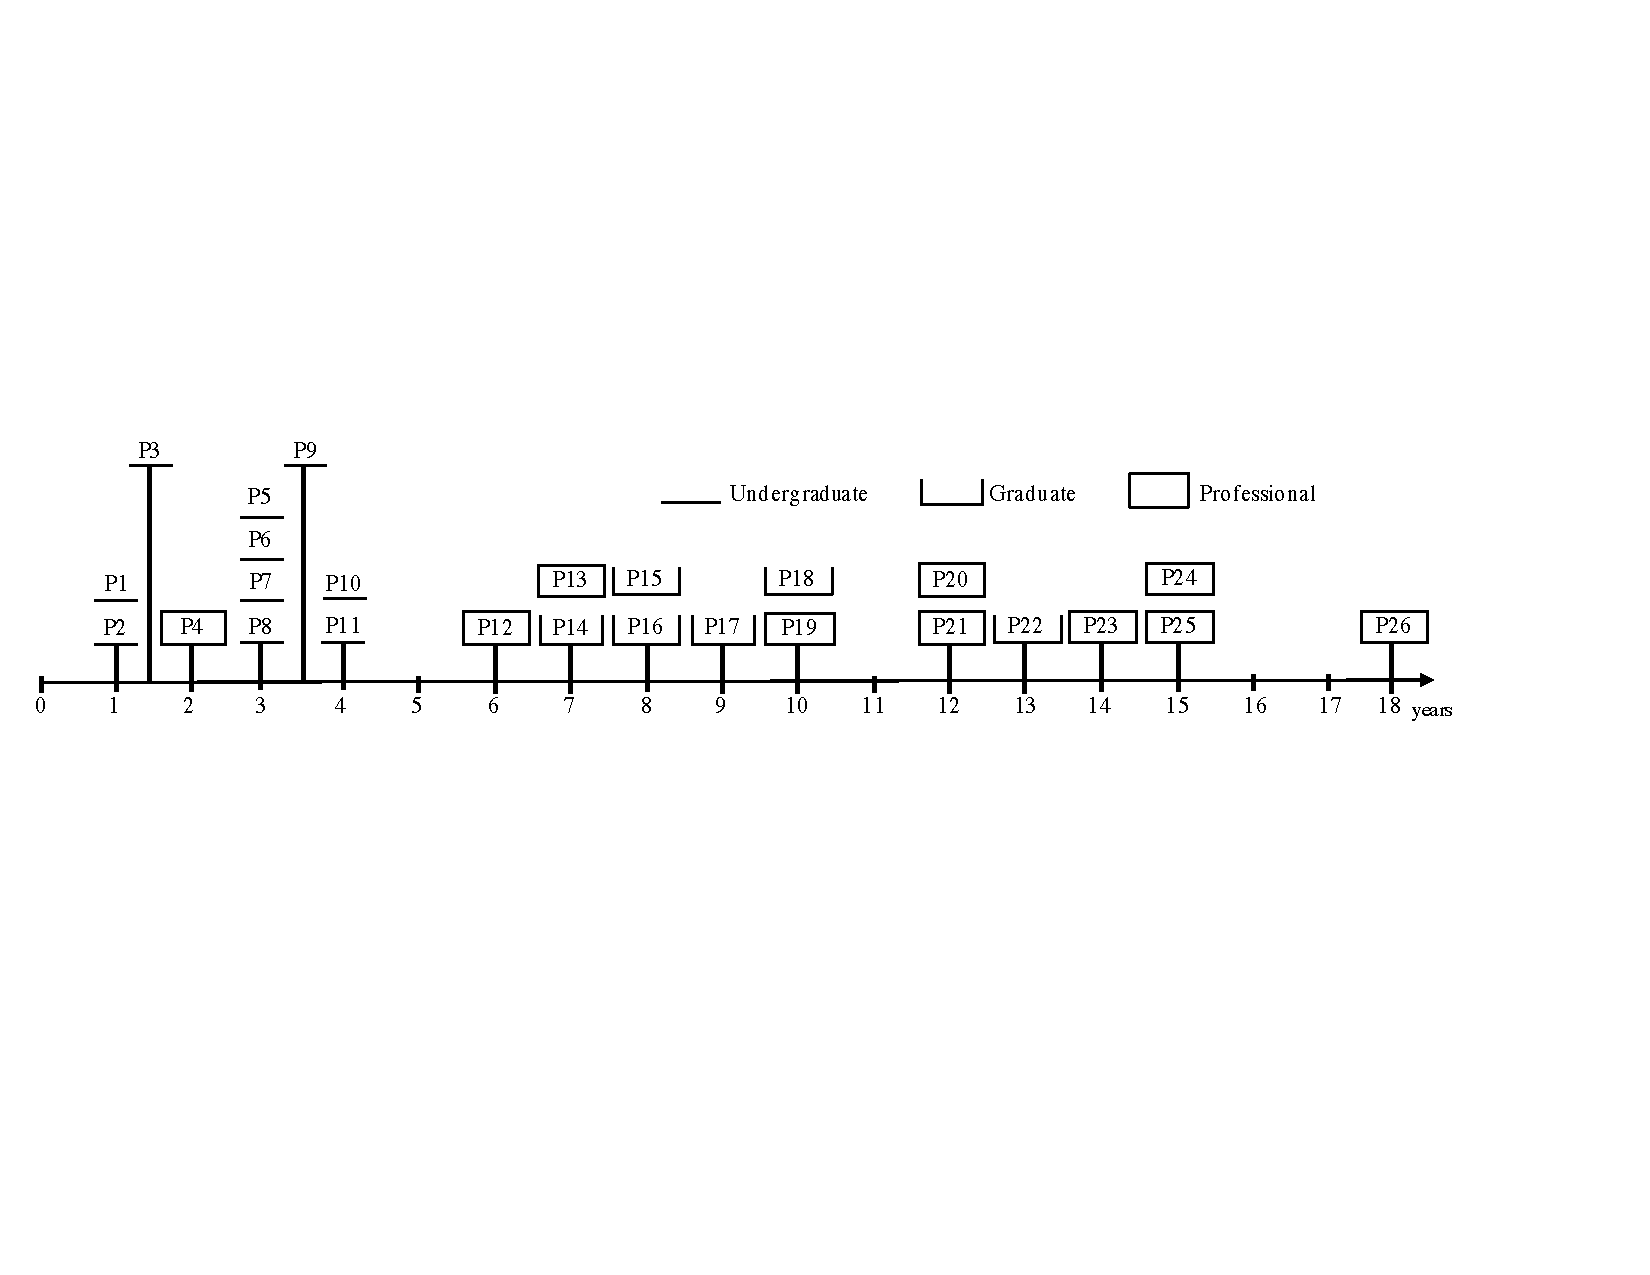
\includegraphics[width=\textwidth]{Chapter-4/figs/participants.pdf}
\caption{Distribution of participants based on years of programming
experience.}
\label{fig:participants}
\end{figure*}

\subsection{Participants} \label{participants}

I recruited twenty-six participants using mailing lists, classroom recruitment, and personal
contacts. Participants included undergraduate students, graduate students, and
professional developers, with varying amounts of development and tool
usage experience. Figure~\ref{fig:participants} shows the distribution of
participants' development experience, based on self-reports in a pre-study
questionnaire. 
Increasing participant numbers indicate increasing software development experience,
and throughout this chapter, I use \professional{boxes} or \graduate{partial} 
\undergraduate{boxes} to indicate participant job roles (professional, graduate, and undergraduate respectively).
For example, the figure indicates that \professional{P24} is a professional developer with fifteen years of development experience. 
Three graduate students (\graduate{P15}, \graduate{P18}, \graduate{P22}) reported having industry experience.
Ten participants had prior experience using EclEmma. 
Nineteen participants had prior experience with FindBugs. 
All participants had experience with the Eclipse Java compiler.

\subsection{Program Analysis Tools Investigated} \label{TUI}

This study focused on tools that can be used in the Eclipse
Integrated Development Environment (IDE)~\cite{EclipseIDE}. 
I chose Eclipse because it is one of the most widely used IDEs~\cite{Goth:2005:Beware}, 
making it easier to recruit qualified participants,
and because it is compatible with a variety of tools. I selected FindBugs, the Eclipse Java Compiler, and
EclEmma as mature, popular tools.


\subsubsection*{FindBugs}

FindBugs (version 2.0) notifications communicate with the developer about defects in her
code based on code patterns. Bug icons (
\includegraphics[height=9px]{Chapter-4/figs/bug}) in the gutter are colored red
to indicate the ``scariest'' code patterns, orange for ``scary'' patterns, yellow
for ``troubling'' patterns, and blue for ``of concern.'' Text descriptions are
available by hovering over or clicking the 
\includegraphics[height=9px]{Chapter-4/figs/bug} icon as seen in Figure~\ref{fig:N4}.

\begin{figure} [t]
	
	\subfigcapskip = 1pt
	\subfigure[Source Code]{
		\fcolorbox{lightgray}{white}{\parbox{\dimexpr\linewidth-5\fboxsep-2\fboxrule}{
				\centering 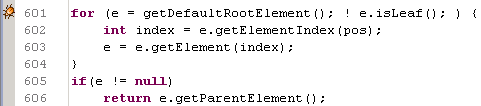
\includegraphics[width =3.3in] {Chapter-4/figs/N4(no_tooltip)}
			}}
			
		}
		
		%The space between the figure and the caption
		\subfigcapskip = 1pt
		\subfigure[Short Description]{
			%From http://tex.stackexchange.com/questions/120530/wrapping-text-inside-framebox
			%\framebox (or fcolorbox) makes the box around the text.  The \parbox allows for wrapping
			%The \dimexpr stuff makes it fit in the column.  You don't need manual
			\fcolorbox{lightgray}{white}{\parbox{\dimexpr\linewidth-2\fboxsep-2\fboxrule}{
					{\centering \scalebox{.8}{Nullcheck of e at line 605 of value previously dereferenced in \texttt{javax.swing.text.DefaultStyledDocument.}}\\
						\scalebox{.8}{\texttt{getParagraphElement(int)} } \\
					}
					
					
				}}
				
			}
			\subfigcapskip = 1pt
			\subfigure[Full Description]{
				\fcolorbox{lightgray}{white}{\parbox{\dimexpr\linewidth-2\fboxsep-2\fboxrule}{
						
						{\centering \scalebox{.8}{A value is checked here to see whether it is null, but this value can't be null because it was previously dereferenced} \\
							\scalebox{.8}{ and if it were null a null pointer exception would have occurred at the earlier dereference. Essentially, this code and} \\ 
							\scalebox{.8}{  the previous dereference disagree as to whether this value is allowed to be null. Either the check is redundant } \\ 
							\scalebox{.8}{or the previous dereference is erroneous.} \\ 

						}
						
						
					}}
				}
				\caption{A notification of a previous null check from FindBugs (FB4).}
				\label{fig:N4}
			\end{figure}

\subsubsection*{Eclipse Java Compiler}

Eclipse Java compiler (JDT version 3.8) notifications communicate with developers when their program cannot
compile and provide warnings about suspicious code~\cite{EclipseCompiler}.
Notifications are typically shown as squiggly underlines in the editor. Like FindBugs, the compiler uses color to represent severity; errors
are shown as red underlines, warnings as yellow underlines.
Underlines are augmented with gutter icons
(
\includegraphics[height=9px]{Chapter-4/figs/comp-x}), as shown in
Figure~\ref{fig:notificationCOMP} at line 159. When the developer mouses over
the underlined code or the 
\includegraphics[height=9px]{Chapter-4/figs/comp-x} icon, the
notification displays a text description (Figure~\ref{Comptext}). Unlike FindBugs, clicking the gutter icon does not provide a detailed description. Instead, clicking the icon sometimes provides possible fixes that can be automatically applied to the code called quick fixes.

\begin{figure} 
\subfigcapskip = 1pt
\centering
\subfigure[Source Code]{
   \fcolorbox{lightgray}{white}{\parbox{\dimexpr\linewidth-2\fboxsep-2\fboxrule}{
	 \centering 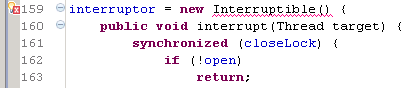
\includegraphics[width=3.3in]{Chapter-4/figs/comp-notification}
	
}}}
\subfigcapskip = 1pt
\subfigure[Text Description]{
\fcolorbox{lightgray}{white}{\parbox{\dimexpr\linewidth-2\fboxsep-2\fboxrule}{
	
{\centering \scalebox{.8}{The type \texttt{new AbstractInterrruptibleChannelInterruptible()} must implement the inherited abstract  } \\
  \scalebox{.8}{\texttt{method new AbstractInterruptibleChannel.Interruptible.interrupt()}}
}


}} }

\caption{An Eclipse compiler notification about unimplemented methods (CMP5).}
\label{fig:notificationCOMP} 
\end{figure}

\subsubsection*{EclEmma}

EclEmma (v2.2) is a code coverage tool that executes a program, typically with JUnit
as the driver~\cite{JUnit}, to communicate with the developer about code paths that did and
did not get exercised. Although EclEmma communicates about one particular execution, 
as with the other tools it provides information to the developer regarding code 
(during runtime rather than compile-time). 
EclEmma uses highlighting to indicate code execution; code highlighted in
green was executed, red was not executed, and yellow was partially executed.
Figure~\ref{fig:notificationECL} shows an example of coverage reported by
EclEmma on an \texttt{if} statement. When the developer mouses over the

\includegraphics[height=9px]{Chapter-4/figs/diamond} icon, the tool notifies her of how many
paths got executed on the associated branch statement at line 133
(Figure~\ref{Ecltext}).

\begin{figure} [t]
\subfigcapskip = 1pt
\centering
\subfigure [Source Code with Highlighting]{ 
\fcolorbox{lightgray}{white}{\parbox{\dimexpr\linewidth-2\fboxsep-2\fboxrule}{
    \centering 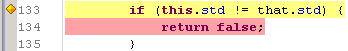
\includegraphics[width=3.3in]{Chapter-4/figs/EclExample}
	
}}}
\subfigcapskip = 1pt
\subfigure[Text Description]{
\fcolorbox{lightgray}{white}{\parbox{\dimexpr\linewidth-2\fboxsep-2\fboxrule}{
	\centering
	{\small ~~~1 of 2 branches missed~~~ }
   
}}
}

\caption{An EclEmma notification about partial branch coverage (ECL3).}
\label{fig:notificationECL}
\end{figure} 

These tools may seem quite different, but I chose them
specifically to identify challenges developers experience \emph{across} tools.
Despite the differences, these tools attempt to communicate similar concepts to developers using similar textual and visual notifications.
For example, both FindBugs and EclEmma communicate information about 
control flow, and both FindBugs and the Eclipse Java Compiler communicate about data flow.
All three tools use color codes in a largely consistent manner, 
such as using red to indicate the highest level of urgency.
And as a final example, most notifications communicate information about program elements, such as methods and classes, and information about program execution, be it potential or actual.


\begin{table*} 
\rowcolors{2}{white}{gray!25}
\centering
\caption{Notifications used in our study}
\begin{tabular}{llll}
%\rowcolor{gray!50}
	\hline
    \textbf{Notification} & \textbf{Tool} & \textbf{Problem} & \textbf{Category} \\
	\hline

%tildes just padding out to \textwidth
    FB1~~~~~~~~~~~~~~~~~& FindBugs~~~~~~~~~~~~~~& \begin{tabular}[c]{@{}l@{}}String comparison \\using == or !=\end{tabular}~~~~~~~~~~~~& Pointers/References\\
    FB2			    & FindBugs      	  		& \begin{tabular}[c]{@{}l@{}}Incorrect Lazy \\ Initialization\end{tabular} 		    			& Multi-threading		\\
    FB3 				& FindBugs     		  		& \begin{tabular}[c]{@{}l@{}}Synchronize on \\ mutable field\end{tabular}						& Multi-threading	    	\\
    FB4				& FindBugs     		  		& \begin{tabular}[c]{@{}l@{}}Redundant null check\end{tabular} 									& Null/Pointers/References	     	\\
    FB5				& FindBugs       	  		& \begin{tabular}[c]{@{}l@{}}Possible null \\pointer dereference\end{tabular}						& Null/Pointers/References		\\
    CMP1				& Eclipse Compiler    & \begin{tabular}[c]{@{}l@{}}Unused code\end{tabular}							    				& Dead Code	\\
    CMP2				& Eclipse Compiler    & \begin{tabular}[c]{@{}l@{}}Unchecked Conversion, \\Raw Type\end{tabular}							& Generics              \\
    CMP3				& Eclipse Compiler    & \begin{tabular}[c]{@{}l@{}}Unimplemented methods\end{tabular}									& Inheritance/Polymorphism	  		 \\
    CMP4			    & Eclipse Compiler    & \begin{tabular}[c]{@{}l@{}}Serializable class \\needs serial ID\end{tabular}						& Serialization	              \\
    CMP5			    & Eclipse Compiler    & \begin{tabular}[c]{@{}l@{}}Unimplemented methods\end{tabular} 									& Inheritance/Polymorphism	          		\\
    CMP6    			& Eclipse Compiler    & \begin{tabular}[c]{@{}l@{}}Method not applicable \\for arguments\end{tabular}						& Inheritance/Polymorphism	            \\
    ECL1				& EclEmma		      		& \begin{tabular}[c]{@{}l@{}}Red class with \\red class header\end{tabular} 					& Class/test coverage	        	\\
    ECL2				& EclEmma       	  		& \begin{tabular}[c]{@{}l@{}}Red class \\(constructor only)\end{tabular}						& Class/test coverage	            	\\
    ECL3				& EclEmma       	  		& \begin{tabular}[c]{@{}l@{}}Simple if statement\end{tabular}								& Branch/test coverage	   		\\
    ECL4				& EclEmma       	 		& \begin{tabular}[c]{@{}l@{}}Return statement \\with branches\end{tabular}					& Branch/test coverage                \\
    ECL5				& EclEmma			  		& \begin{tabular}[c]{@{}l@{}}Try/Catch/Finally \\(coverage varies)\end{tabular}				& Test coverage, Exception handling	           	 \\
    ECL6				& EclEmma       		 	& \begin{tabular}[c]{@{}l@{}}Nested if statements\end{tabular}								& Branch/test coverage              \\
    \hline
\end{tabular}
\label{table:notifications}
\end{table*}

\subsection{Study Protocol}

Each session with a participant lasted approximately one hour.
Prior to each session, participants filled out a consent form
and pre-questionnaire.\footnote{This work was approved under IRB No. 2787.} 
Each session consisted of seventeen tasks.

Source code for the tasks came from OpenJDK~\cite{OpenJDK} and JFreeChart~\cite{JFreeChart}.
I chose Open JDK because it has a large code base from which I could easily
find bugs using their publicly available FindBugs cloud
report~\cite{FindBugsCloud}. I chose JFreeChart because it is a large code
base with working JUnit test cases that exhibit less-than-perfect code coverage.

For each task, I presented participants with and asked them to interpret one or more notifications from a given tool.
I disallowed the use of a web browser to isolate the challenges developers encounter to the notifications used by the tools and to exclude challenges caused by outside tools or resources.
Allowing use of the browser would have added data that does not help answer the current research question.
I also wanted to see if developers could interpret tool notifications without the aid of outside resources. 
During many tasks, and at least once for every participant, participants
discussed or completed notification resolution. I did not require them to do so as the focus of this study was on the ability to interpret, not to resolve.
As participants explained the notifications, the first author asked follow-up
questions as necessary. 

% EDITED BASED ON REVIEWER COMMENT
Table~\ref{table:notifications} shows a list of the notification tasks participants encountered during each session. A more detailed listing, with screenshots, of the notifications used in this study can be found in Appendix~\ref{chap4:artifacts}. 
For each task, I chose notifications to represent the types of notifications developers may encounter when programming.
For FindBugs and the Eclipse compiler, I chose notifications that appeared frequently in the OpenJDK project. 
I chose EclEmma notifications from JFreeChart to exercise a range of its coverage scenarios. 
Because EclEmma's documentation did not specify the range of notifications it uses, 
I manually went through JFreeChart's codebase after running the tool and took note of 
each new coverage scenario encountered.
I then included an example of every coverage scenario in the EclEmma tasks.

\begin{figure} 
\subfigcapskip = 1pt
\centering
\subfigure[Source Code]{
   \fcolorbox{lightgray}{white}{\parbox{\dimexpr\linewidth-2\fboxsep-2\fboxrule}{
	 \centering 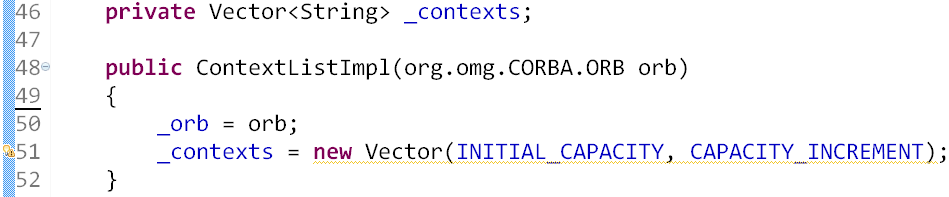
\includegraphics[width=3in]{Chapter-4/figs/CMP2}
	
}}}
\subfigcapskip = 1pt
\subfigure[Text Description]{
\fcolorbox{lightgray}{white}{\parbox{\dimexpr\linewidth-2\fboxsep-2\fboxrule}{
	
{\centering \scalebox{.8}{- Type safety: The expression of type Vector needs unchecked conversion to conform to Vector<String>.}\\
		\scalebox{.8}{- Vector is a raw type. References to generic type Vector<E> should be parameterized.}\\
}


}} }

\caption{A notification from the compiler about generics (CMP2).}
\label{fig:CMP2} 
\end{figure}

For FindBugs, each task during the session corresponded to a single
notification.
All but one compiler task corresponded to a single notification;
because the two notifications on CMP2 (Figure~\ref{fig:CMP2}) contribute to the same problem on the same line, I presented them as one task. 
%TODO explain ``CMP'' notation, as well as participant notation.
Each EclEmma task consisted of participants explaining coverage notifications for the entire class. 

\subsection{Data Collection}

I recorded audio and the screen in each session for analysis.
I then created transcripts from the audio, 
and included descriptions of actions that a participant performed 
that were relevant to interpreting the notification. 
For example, if a participant navigated to different parts of the code 
but did not explicitly describe it, 
I added a description of that navigation to the transcript.

\subsection{Data Analysis}

I analyzed each session using open and selective coding~\cite{corbin2014basics} to discover participant challenges. 
To identify a challenge, I needed concrete criteria. 
I proposed that tool use is a form of communication, and therefore that challenges when interpreting a notification can be seen as ineffective communication.
Existing research on how computers should talk to people suggests that if an explanation is required for a message to be understood, the message was not effective~\cite{dean1982computer}.

I used this logic to determine when a challenge occurred, using three criteria for inclusion: 
\begin{enumerate}
    \item The participant explicitly stated a challenge.
    \item The participant was unable to explain the notification.
    \item The participant had to take steps, outside of reading the notification, to deduce the problem.
\end{enumerate}

Whether an observation met a criterion is independent of whether the participant was able to explain the notification.

I and a collaborator individually used open coding on each transcript, labeling portions that mapped to a challenge. We then reconvened to merge our codes. The criteria above guided this process; if we could not agree that a code fit our criteria, we removed it from our data set. 
Of the 404 codes we originally extracted, we disagreed on 82 (20\%) from twenty-six sessions. 
To resolve our disagreements, we referred to our criteria; if we could not come to an agreement regarding the code fitting the criteria, we removed the statement from our data set. 
For four sessions, we had no disagreement.
In the end, we identified 322 codes. We put each code onto a note card, along with the participant and tool being used. 

Next, I used a card sorting methodology similar to that of Mu\c{s}lu and
colleagues~\cite{Muslu:2014:Transition}. 
The goal of this card sort was to identify themes based on the identified codes.
I used five of the eight authors on the publication of this work and completed the card sort in three phases. In phase 1, we sorted all cards into high-level themes; each card could only go in one theme. s
Phase 2 focused on determining where high-level themes could be broken down into lower-level themes.
In phase 3, we focused on making sure that each card was in the best fitting theme. During this phase, we also clarified theme definitions and made note of example statements to represent each theme.

Because one of the criteria is participant inability to explain a notification, 
any actions or statements made surrounding that occurrence was included in the card sort. 
Upon reflection, some emergent themes took the form of consequences rather than challenges, 
such as notification resolution without understanding and lack of trust in the tool, 
therefore I will not discuss them in this chapter. 
I likewise will not discuss the emergent theme of tool feature requests.
% TODO isthis another appendix??
These excluded themes are available with the other on-line research materials.

\subsection{Study Credibility \& Findings Validation}

There are inherent threats to the validity of empirical 
research~\cite{onwuegbuzie2007validity}.
Despite these inherent threats, prior research suggests there are ways
we can increase confidence in the credibility and validity of empirical
findings~\cite{gasson2004rigor,li2004trustworthiness}.
Following the safeguards for conducting empirical research proposed by
Li~\cite{li2004trustworthiness}, I ensured the following in the collection,
interpretation, and reporting of the data I collected:
\begin{itemize}
	\item \textit{Voluntary participation and anonymity.} To receive truthful
	responses from participants, I provided participants up-front with information
	regarding the purpose of the study, what will happen with the data, and how
	anonymity will be ensured.
	\item \textit{Purposeful sampling.} To sample with the purpose
	of gathering diverse participants and to increase
	the ability to generalize findings, I recruited participants from
	academia and industry with varying levels of programming experience.
	\item \textit{Triangulation.} To increase reliability, I triangulated data from direct observation and think aloud.
	\item \textit{Prolonged engagement.} 
	To allow participants time to get acclimated to a researcher being present
	while not getting too fatigued to contribute data,
	each session lasted about one
	hour. To increase the effectiveness
	of this safeguard, the researcher interrupted as little as possible.
	\item \textit{(Near-) Natural situation.} 
	To increase ecological validity, I set up the study environment and
	recruited participants familiar with that environment and programming language.
	I also allowed participants to explore the code as they would if it were their
	own.
	\item \textit{Peer debriefing, stepwise replication, and interrater reliability.} 
	To ensure researcher agreement about the findings, two authors separately 
	analyzed the transcripts for statements of interest. 
	I also included multiple researchers
	throughout the multi-step analysis and reporting process.
	\item \textit{Member checks.} To ensure validity of
	the data and our interpretation, I reached out to all participants, providing
	them with a summary of the findings, a copy of the written report, and a form
	for providing feedback on the findings.
	\item \textit{Thick description.} To enable judgment of how my research fits with other contexts, we describe in detail the methods used to collect the data and the setting in which it was collected.
\end{itemize}

Other safeguards include \textit{Training for subjects}, \textit{Background checks}, and \textit{Refrain from generalizing}. I did not conduct training for think aloud, as it could have affected my ability to recruit participants. I used criteria for participation as a background check and do not generalize outside the context of software developers.
%We use our themes and sub-themes in Section~\ref{sec:results} to organize our results.

\def\toggle{
	\begin{scope}[ocg={name=test2, ref=t2, status=visible}]
		\node[inner sep=0pt] (svgPDF) at (0,0)
		{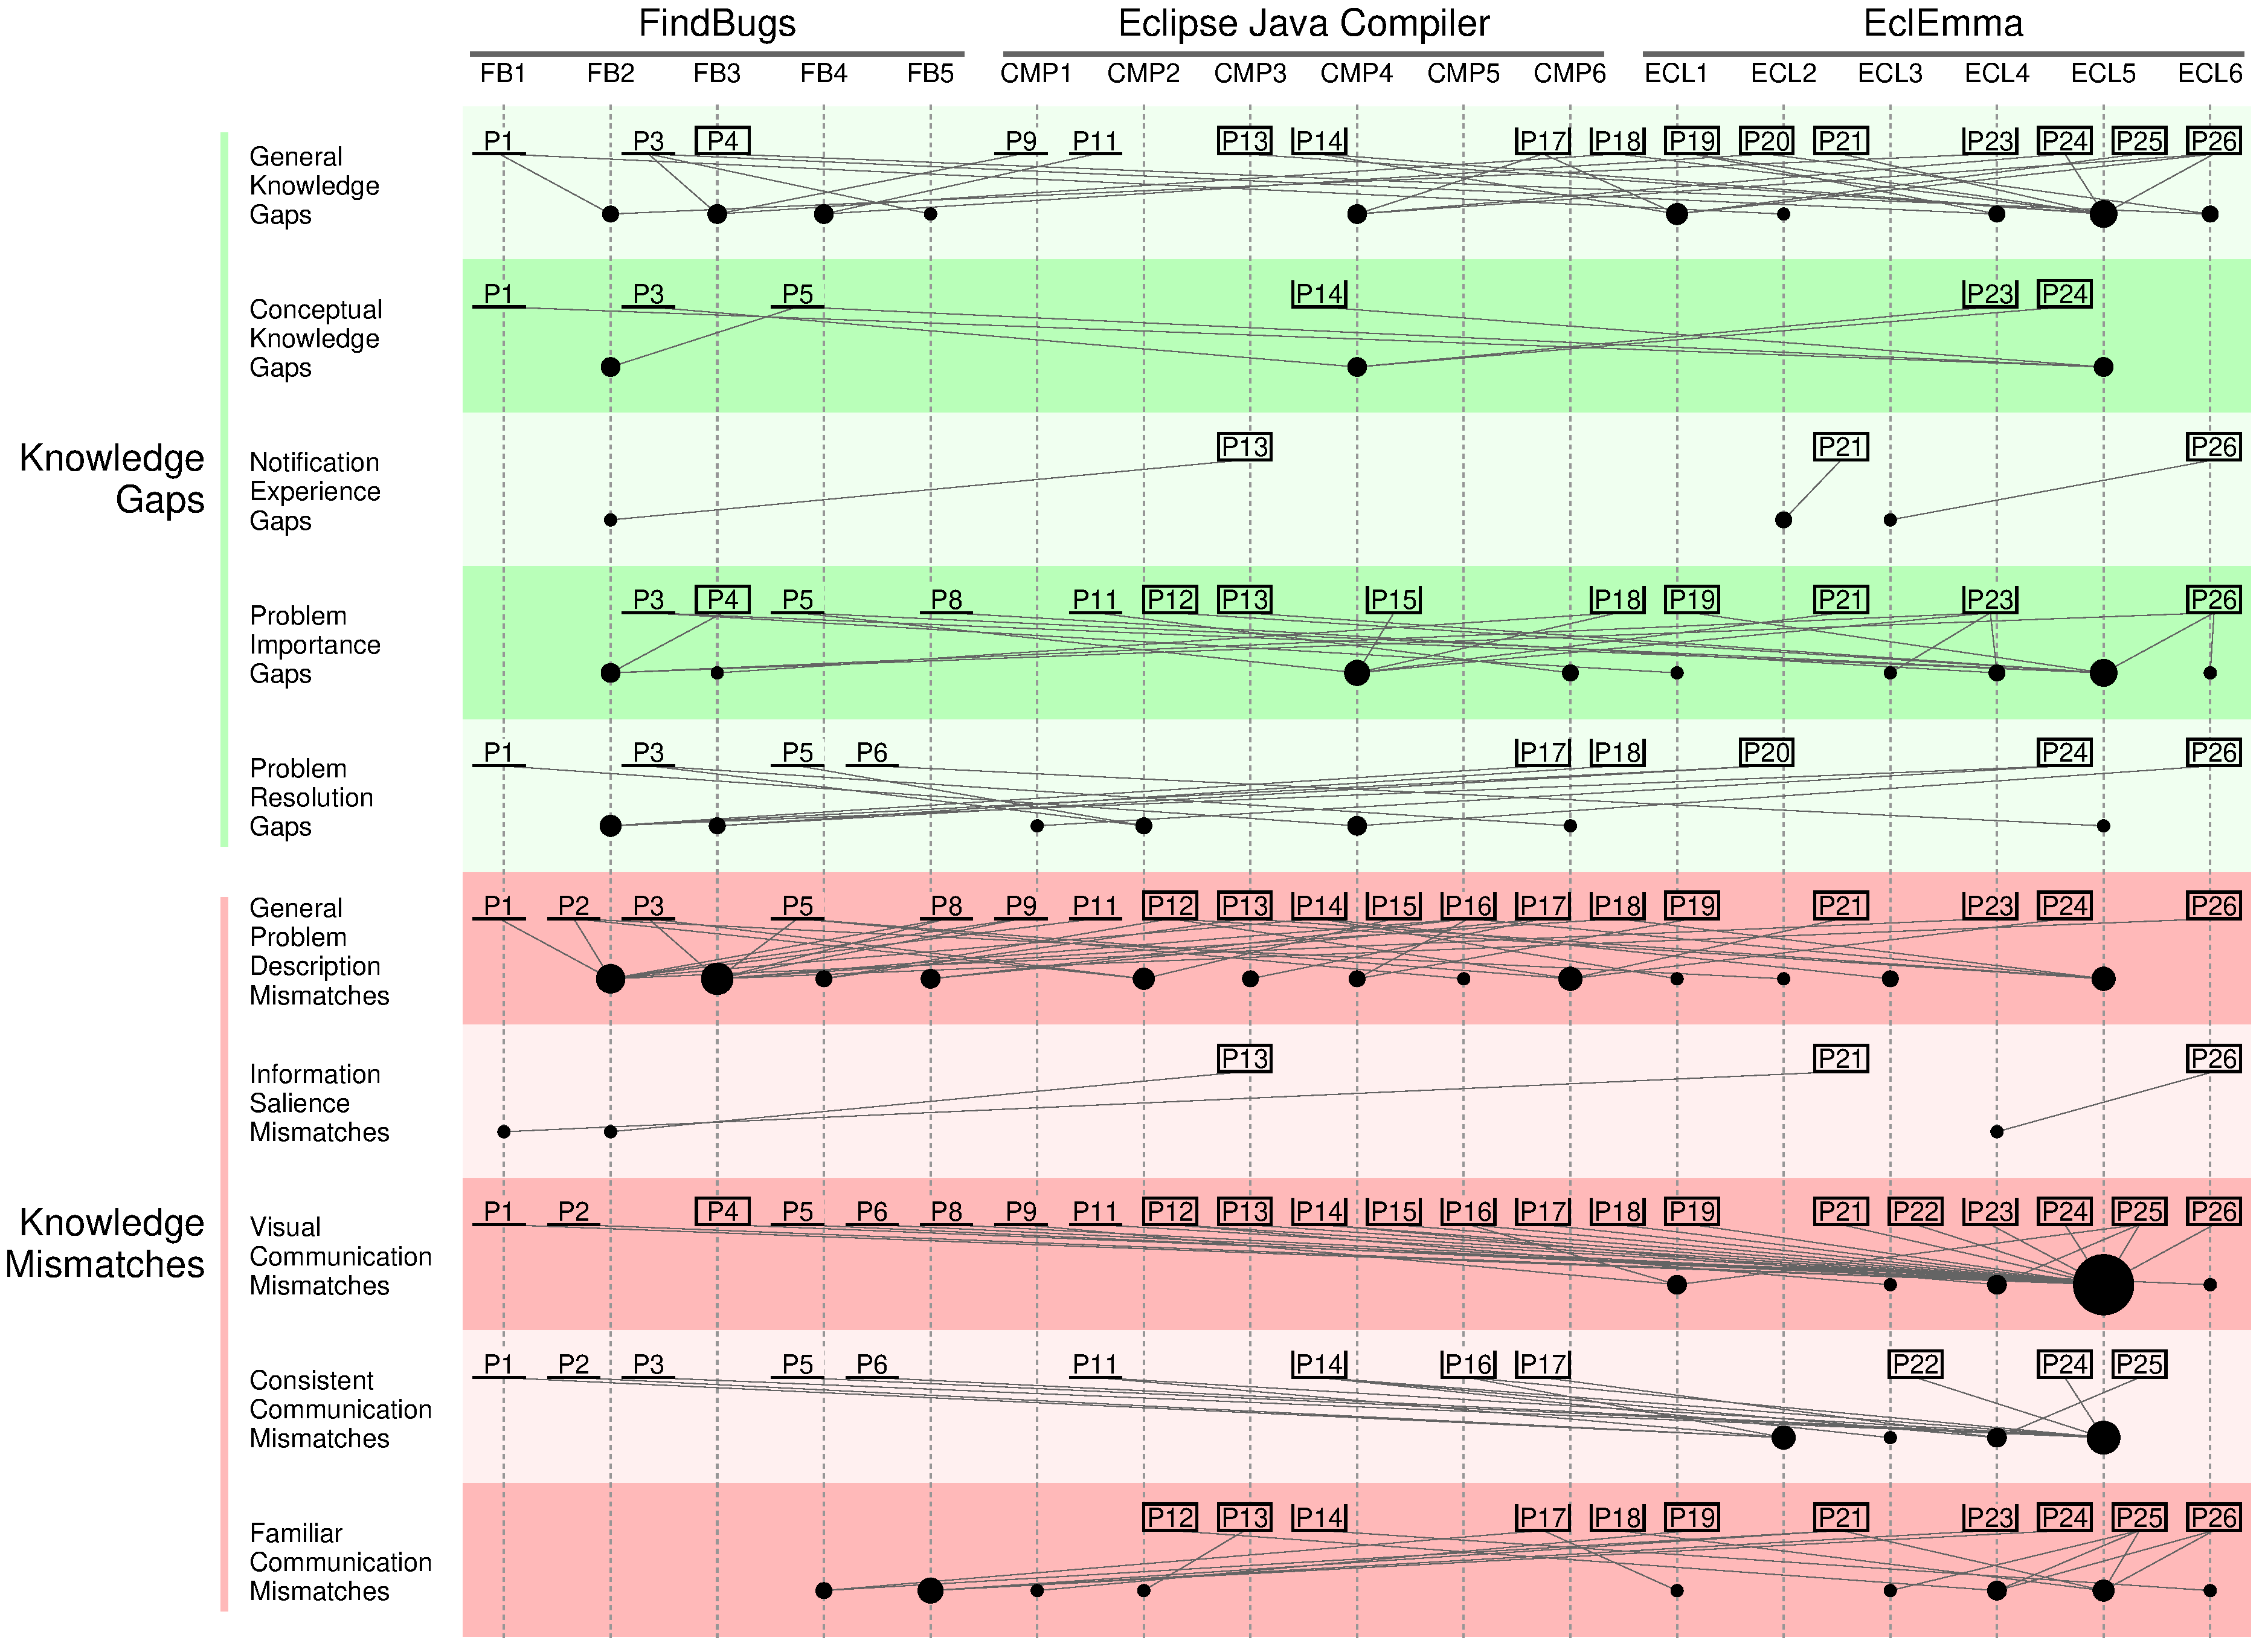
\includegraphics[width=\textwidth]{Chapter-4/figs/Issues_Full.pdf}};
	\end{scope}
	\begin{scope}[ocg={name=test1, ref=t1, status=invisible}]
		\node[inner sep=0pt] (svgPDF) at (0,0)
		{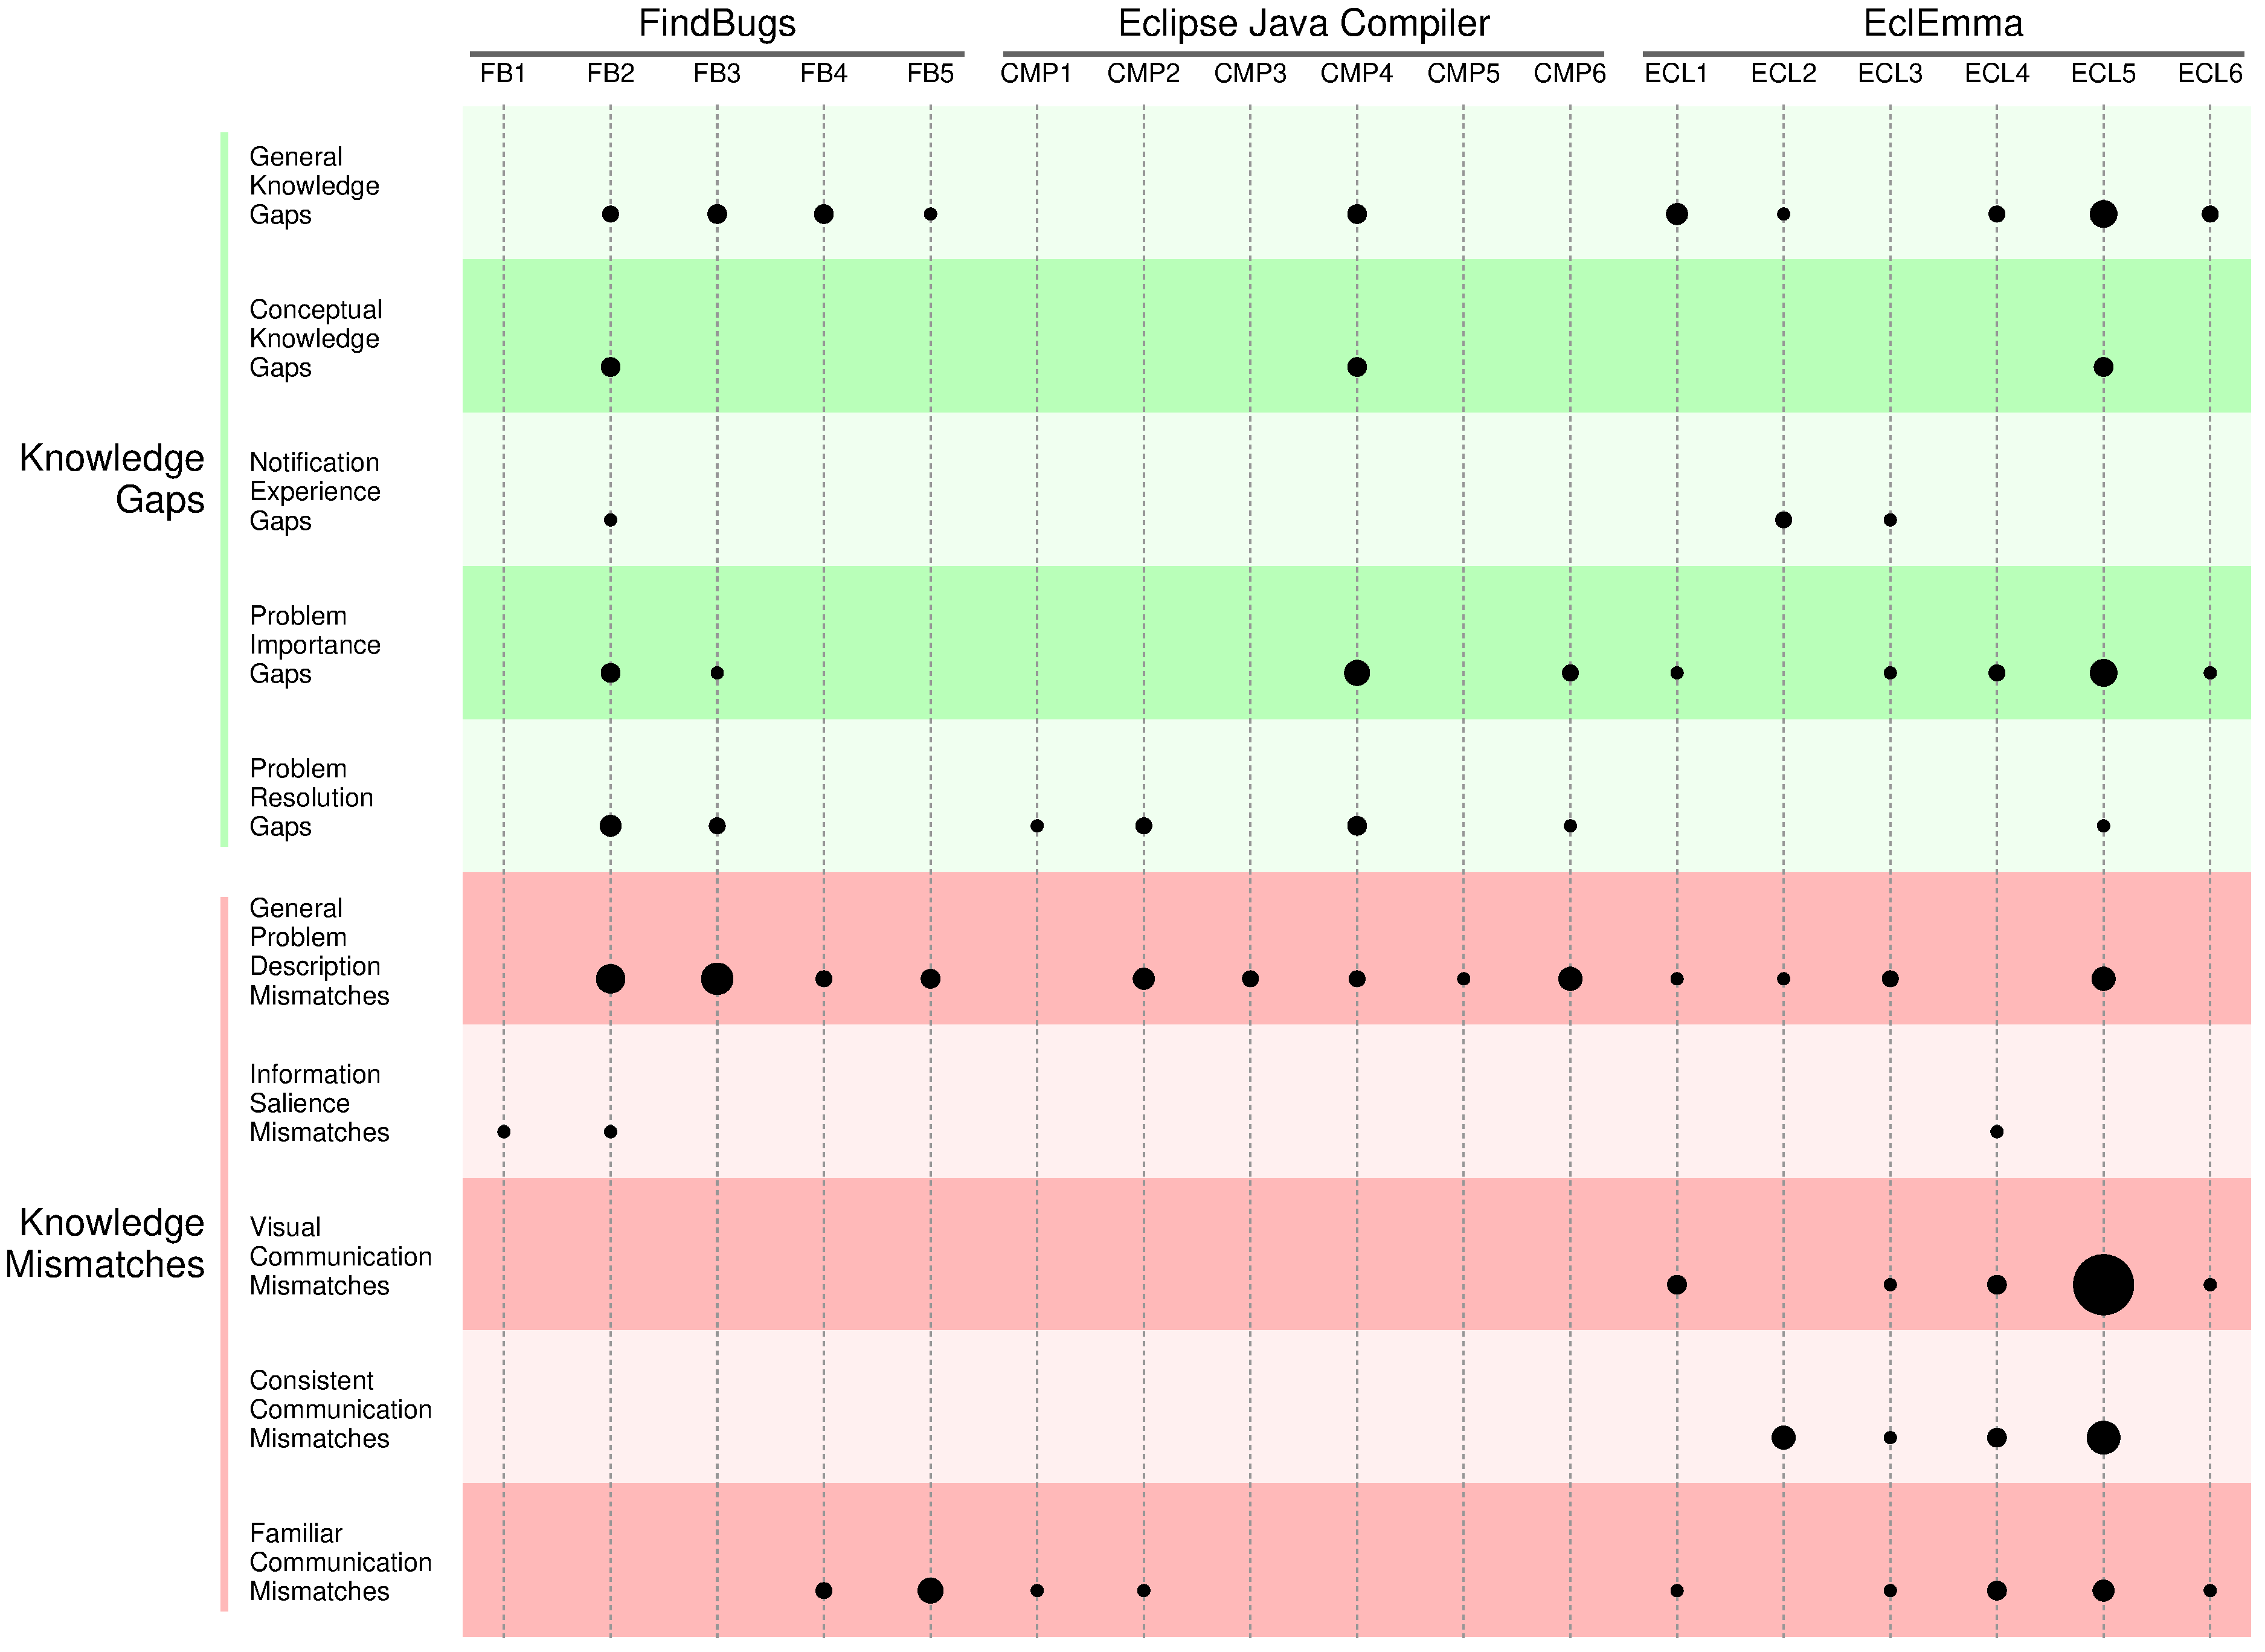
\includegraphics[width=\textwidth]{Chapter-4/figs/Issues_Challenges.pdf}};
	\end{scope}
	\node[draw,switch ocg={t1 t2}] at (0,-6.8) {Hide/Display Details};
}


%\begin{figure*}[ht] \centering \includegraphics[width=7in]{figs/results.pdf}
%\caption{Distribution of difficulties encountered and notifications that caused them.}
%\label{fig:results}
%\end{figure*}

\section{Knowledge-Related Challenges}

Remember Valerie from Chapter~\ref{chap-one}? Though she is a hypothetical developer, the challenges she faced are not hypothetical. Valerie experienced challenges caused by both knowledge gaps (no knowledge regarding lazy initialization) and knowledge mismatches (expecting an explicit connection to synchronization). 
Because research suggests experience matters when understanding vulnerabilities, and that experiences affect knowledge, I speak about knowledge here and throughout this thesis as the culmination of experiences~\cite{johnson1989mental,argote2011organizational,baca2009static}.
Using that definition, a \emph{knowledge gap} occurs when there is a gap between what the developer knows, based on her experiences, and how the tool communicates; a \emph{knowledge mismatch} occurs when what the developer knows and expects from the tool, based on her experiences, does not match the notification the tool uses.

% Based on this theory, I hypothesize that if it was possible for tools to be aware of what developers know and do not know, tools can improve communication by adapting its notifications to the developer.

\def\toggle{
	\begin{scope}[ocg={name=test2, ref=t2, status=visible}]
		\node[inner sep=0pt] (svgPDF) at (0,0)
		{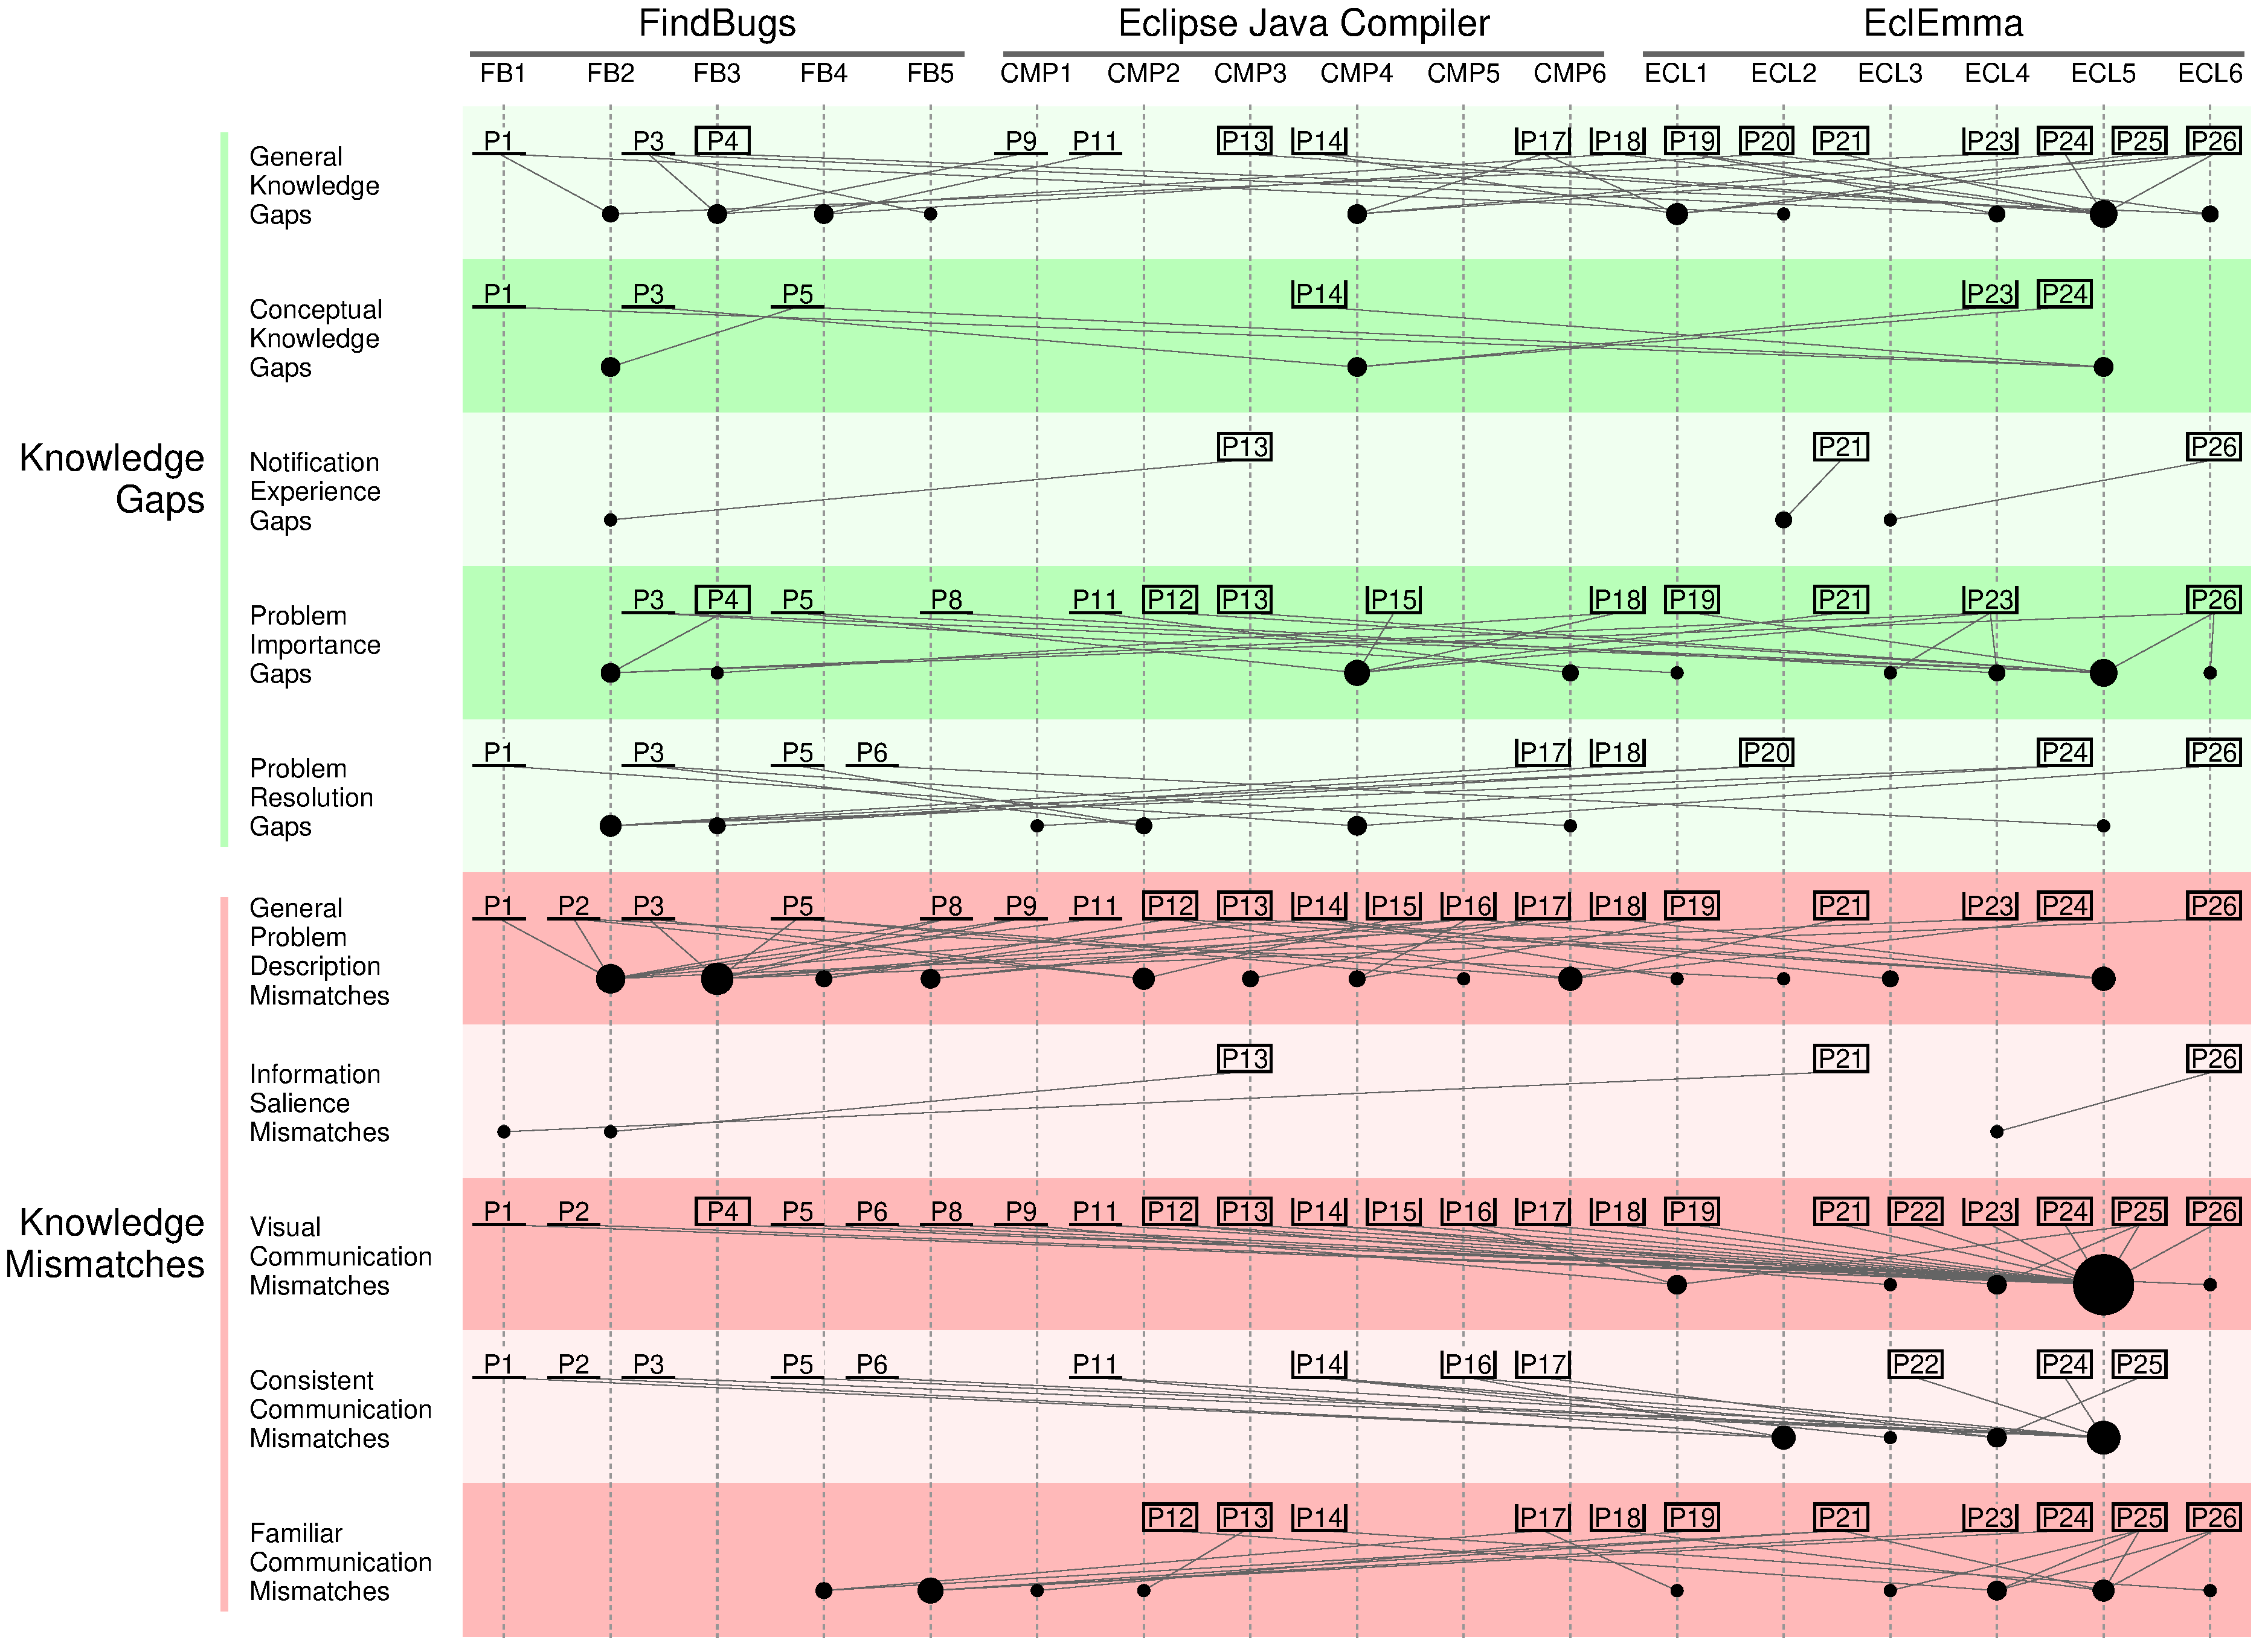
\includegraphics[width=\textwidth]{Chapter-4/figs/Issues_Full.pdf}};
	\end{scope}
	\begin{scope}[ocg={name=test1, ref=t1, status=invisible}]
		\node[inner sep=0pt] (svgPDF) at (0,0)
		{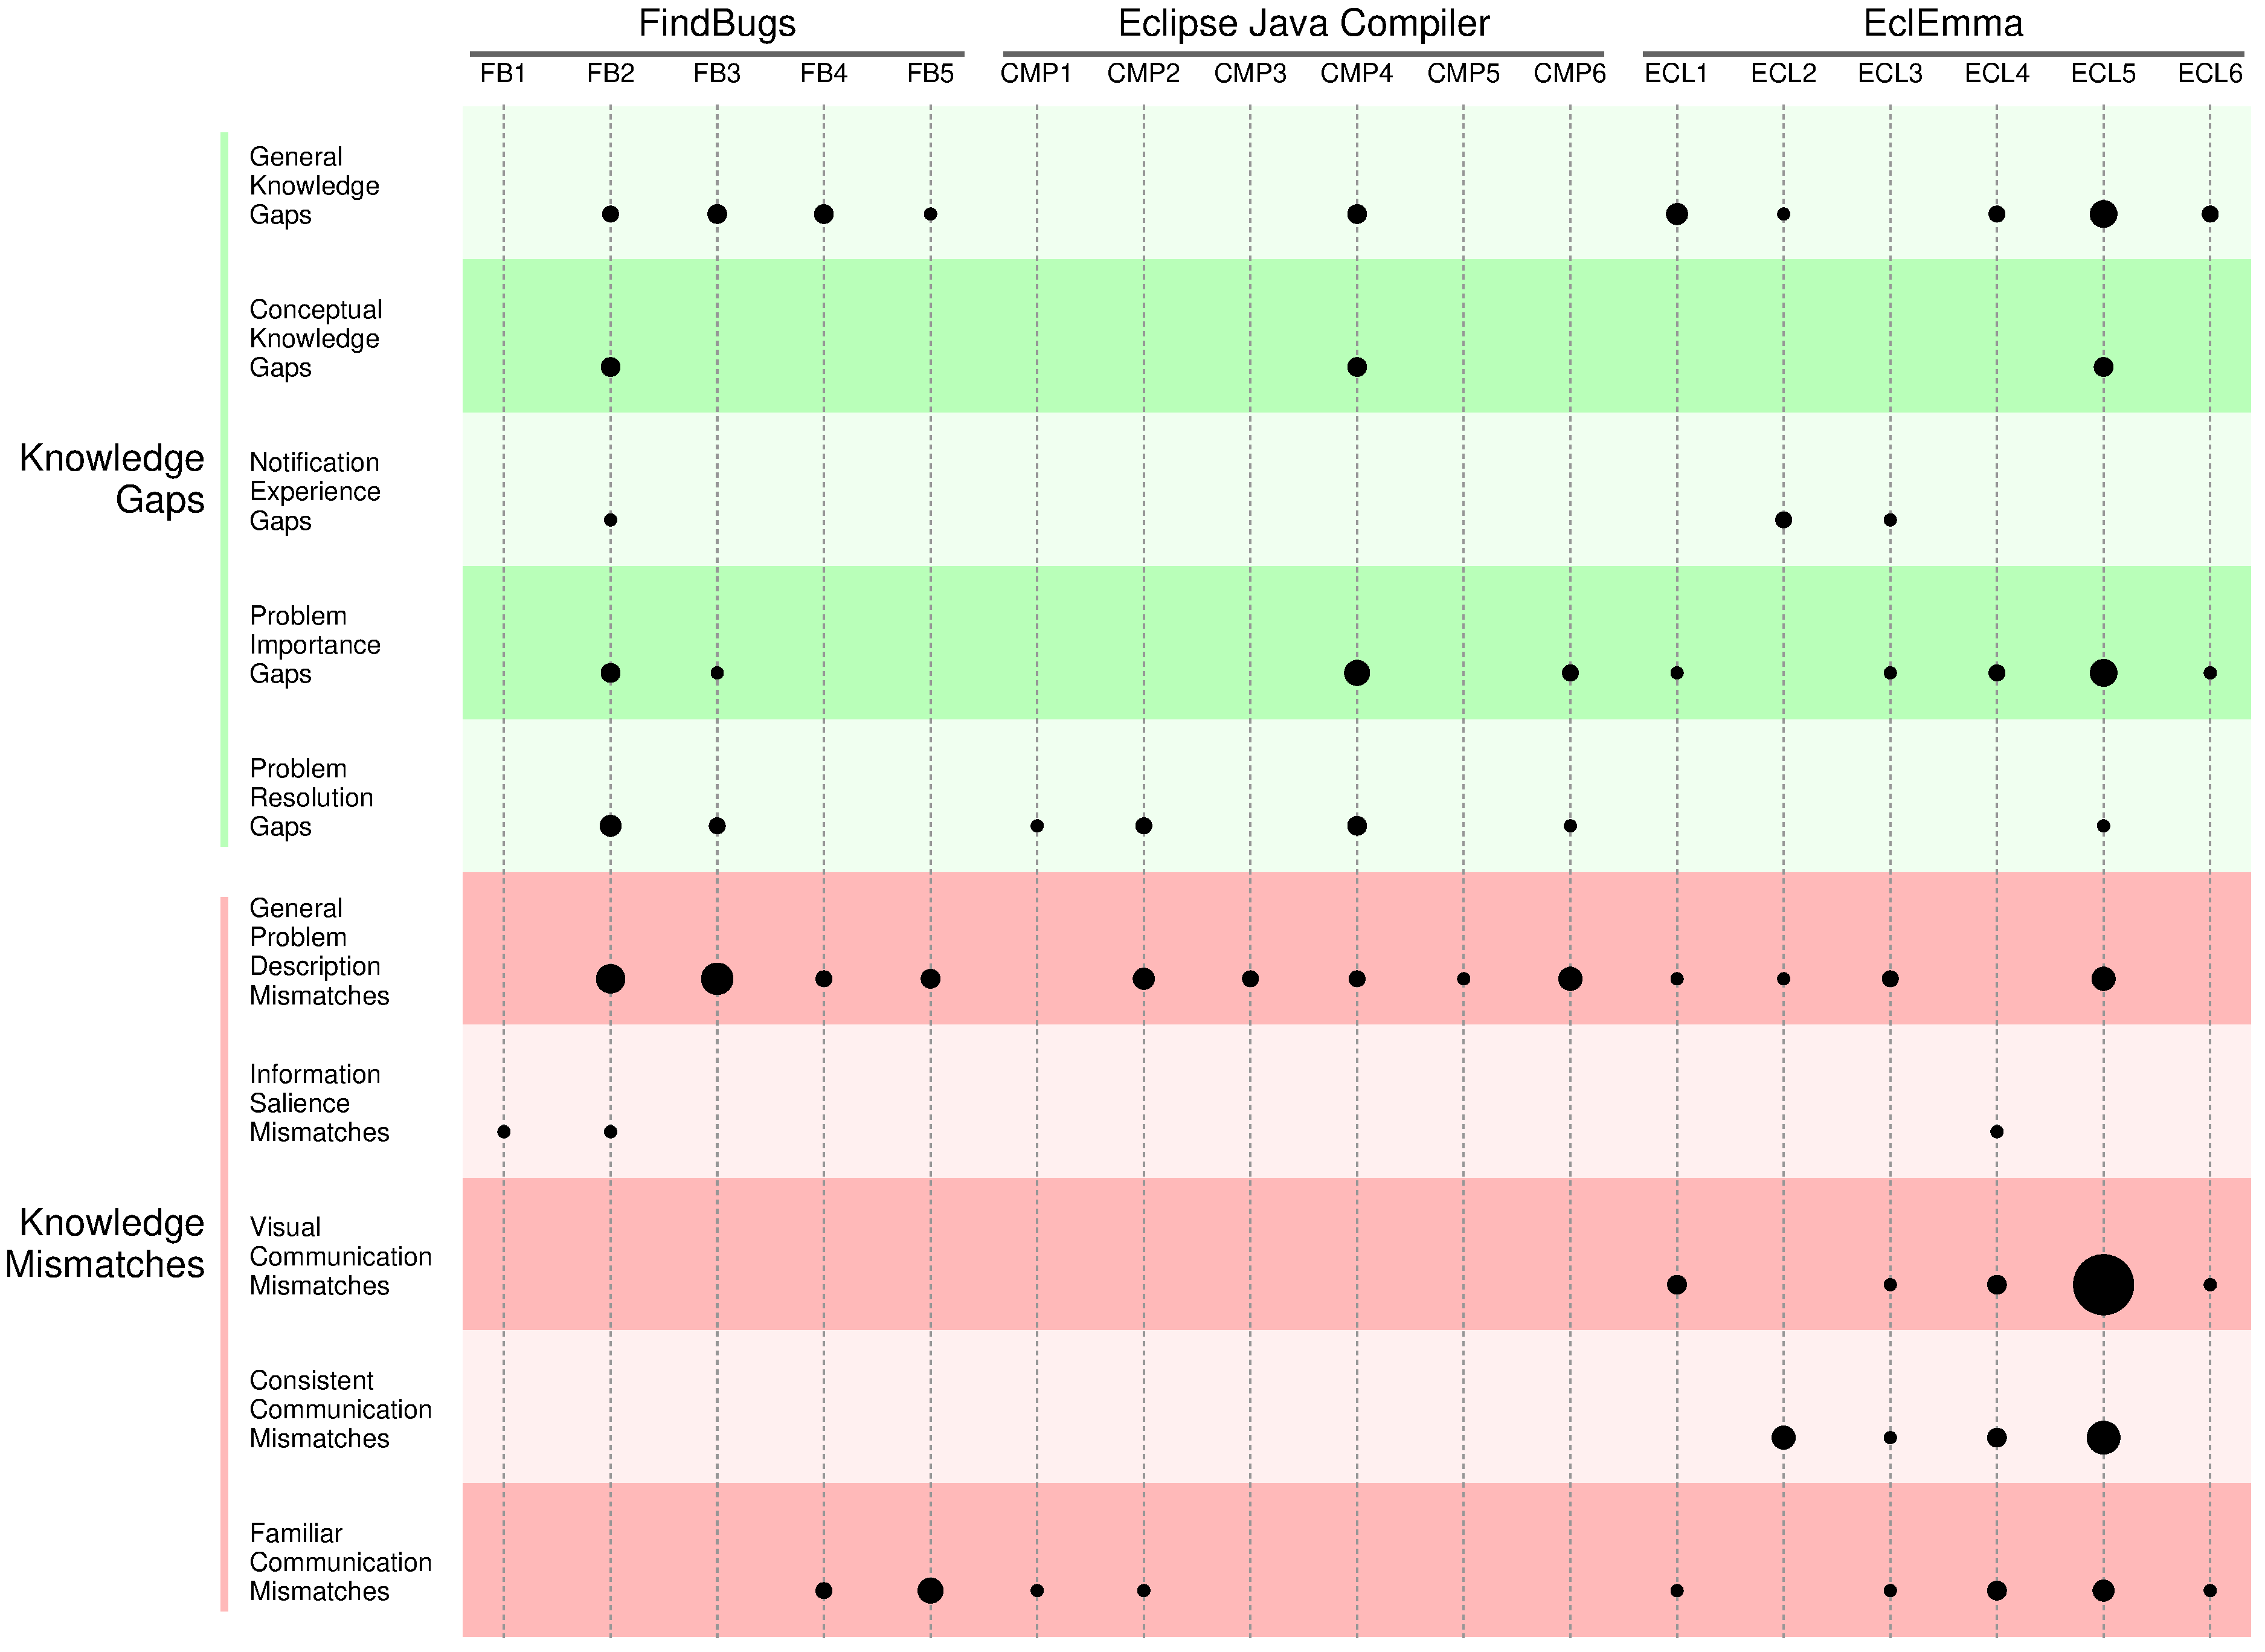
\includegraphics[width=\textwidth]{Chapter-4/figs/Issues_Challenges.pdf}};
	\end{scope}
	\node[draw,switch ocg={t1 t2}] at (0,-6.8) {Hide/Display Details};
}

\begin{figure*}[ht]
	\centering
	\begin{tikzpicture}
	\toggle
	\end{tikzpicture}
	\caption{Distribution of challenges encountered and notifications that caused them.}
	\label{fig:results}
\end{figure*}

The challenges that comprise my theory are 
shown in Figure~\ref{fig:results}.
Vertical lines represent the tasks and the horizontal bars indicate challenges.
The area of the dots indicate how many participants encountered challenges with that notification in that theme. 
Diagonal lines map participants to the challenges interpreting that notification.
\setlength\fboxsep{1pt}
When opened in Adobe Acrobat, clicking \framebox{``Hide/Display Details''} 
interactively toggles between showing and hiding this mapping.
I describe each challenge type, and validation of the findings, in detail in the remainder of this section.

\subsection{Knowledge Gaps}\label{subsec:gaps}

Knowledge gaps occurred when there was a gap between what participants know and the information provided by the notification. 
Knowledge gap challenges occurred when participants did not have existing knowledge of software 
development activities relevant to a given notification.  
However, we found it is not as simple as ``beginners battle and experts excel'', 
but instead that challenges faced by developers can occur regardless of programming or industry experience. 
In this subsection, I will describe general knowledge gap challenges, followed by four specific kinds of knowledge gaps identified in this study.

\subsubsection{General Knowledge Gaps}\label{subsec:infogap}
General knowledge gap challenges occurred when there was a gap between the general 
software development knowledge participants had relevant to the notification and the 
information provided by the notification.  
When participants did not provide enough information to map a challenge to a 
more specific kind of knowledge gap, I placed that challenge in this theme.
Participants experienced knowledge gap challenges across all three tools (Figure~\ref{fig:results}). 

FindBugs was more dominant in this theme than the compiler, with 9 and 2 participants encountering challenges respectively. This was the case, despite the compiler using less text than FindBugs to communicate. Participants focused on the text to understand the problem, but struggled to understand what the tool was trying to convey. Despite FindBugs' verbosity, as stated by 4 participants, the tool provided just enough to need to use the web to figure out the problem. For example, \professional{P25} struggled to interpret FB3. He made an effort to understand the notification, but then realized the notification did not provide enough for him to feel confident in his explanation, stating:

\vspace{0.5em}
\begin{quote}
	\textit{I would definitely want to correct it but I don't get enough info from here to know what to correct or what I did wrong so I would probably take this message and go to Google to see if anybody else is talking or saying something that I understand better.}
\end{quote}

\noindent
Participants who struggled with compiler and EclEmma notifications found themselves in a situation similar to \graduate{P17} when interpreting CMP4 and notifications in ECL1. When he encountered CMP4 and ECL1, he immediately realized the notifications did not provide enough information for him to come to a conclusion about each. He noted, like \professional{P25}, that he would need to use Google or documentation to better understand the notification being provided. \graduate{P17} was unable to come to a conclusion regarding either notification.
% some challenges that emerged clarify the types of information gaps developers may experience based on knowledge they have not, but would like to acquire

These findings confirm that more is not always better~\cite{Nienaltowski:2008:Compiler} for closing knowledge gaps and that these gaps exist with visual communication as well.
Along with general knowledge gap challenges, participants experienced challenges caused by four specific types of knowledge gaps that emerged: \textit{conceptual knowledge gaps}, \textit{notification experience gaps}, \textit{problem importance gaps}, and \textit{problem resolution gaps}.

\subsubsection{Conceptual Knowledge Gaps}\label{subsec:concept}
% challenge caused by no experience with concept
Conceptual knowledge gaps occurred when there was a gap between participants' knowledge of programming concepts, 
like serialization, present in the notification and the information provided by the notification regarding those concepts. 
\professional{P24}, a professional developer with 15 years of experience, attempted to work through 
CMP4 despite his unfamiliarity with serialization. 
His guess, based on the notification, was that he was missing a \texttt{serialversionUID}; 
however, beyond that he was unsure how a \texttt{serialversionUID} is associated with serialization. 
This led to the inability for \professional{P24} to fully interpret the notification.

\undergraduate{P5} encountered challenges interpreting FB2 due to conceptual knowledge gaps regarding multi-threading. 
The notification spoke about concepts such as lazy initialization, which \undergraduate{P5} noted he had not had past experience with. 
herefore, he could only guess what was wrong with the code.

Conceptual knowledge can also affect visual communication, even when the relevant concepts are not depicted in the notification. Test coverage is the obvious concept necessary to understand test coverage notifications. 
Some of the notifications participants encountered from EclEmma required knowledge of other concepts, such as exception handling. 
Three participants noted they could not confidently explain EclEmma notifications involving \texttt{finally} blocks using the visuals provided due to their minimal experience with \texttt{finally} blocks.

After completing ECL5, most participants could at least vaguely explain the notifications they encountered. 
However, \undergraduate{P5} still could not definitively conclude anything about the notifications, stating: 

\begin{quote}
	\textit{I don't know what \texttt{finally} means but it seems like everything inside \texttt{try} 
	is not getting called\ldots I assume \texttt{finally} is similar to \texttt{catch} 
	but I don't really know how \texttt{finally} works.}
\end{quote}

\noindent
His lack of knowledge regarding \texttt{finally} blocks made it challenging for \undergraduate{P5}, 
despite his familiarity with other relevant code structures\footnote{The reader may also find this confusing, but this was a design decision made by EclEmma's toolsmiths. This confusion arises from a difference between the bytecode representation and the source code representation of \texttt{finally} blocks (\url{https://github.com/jacoco/jacoco/issues/15}). Although this may seem like a design problem, we included the notifications we did, including ECL5, because they are encountered in the wild.}. 
This, coupled with being his first experience with EclEmma notifications, led to his inability to interpret the notifications in ECL5.

\subsubsection{Notification Experience Gaps}\label{subsec:notif}
Notification experience gaps occurred when there was a gap between participants' knowledge gained 
from experience with a notification they encountered for the first time and the notifications they have previously encountered. 
Participants' lack of experience with a notification is the knowledge gap that caused challenges in this theme.
For example, \graduate{P21} struggled to interpret the notifications in ECL2 due to the differences in highlighting on uncovered methods and constructors.  His comments suggested that he understood the concept of coverage, but stated that the challenge was due to unfamiliarity with the tool.
When he first encountered an uncovered method notification, without the signature highlighted like a constructor's signature was, he could not determine whether \emph{lack of highlighting} was equivalent to \emph{red highlighting}.
The challenges in this theme are general in that they relate to overall notification knowledge. Some of the challenges that emerged relate to gaps in knowledge regarding notification specifics, such as importance and resolution. 

\subsubsection{Problem Importance Gaps}\label{subsec:rationale}
% challenge caused by don't know why they should care or why they should resolve, and not mentioned in notification
Problem importance gap challenges occurred when there was a gap between participant knowledge of the importance of the problem and the notification's attempt to communicate importance.
As \graduate{P18} attempted to explain FB3, he realized that although the notification did tell him that he was synchronizing on a mutable field, it did not tell him why that is undesirable. 
He attempted to determine a reason for why it is undesirable, and though he found the notification's message ``unlikely to have useful semantics'' helpful, he noted that his reasoning ``would not be correct'' because he would have to guess.

Without an understanding of why the problem was bad, participants could not confidently interpret the notification; this led to challenges coming up with resolutions. 
For example, \undergraduate{P5} could not confidently resolve CMP4; the notification was clear that a missing \texttt{serialversionUID} is the problem, but did not specify why the ID was needed. 
Though the compiler provided quick fixes, deciding which fix was best for \undergraduate{P5} depended on what the ID was used for, which the notification did not specify.

\subsubsection{Problem Resolution Gaps}\label{subsec:resolution}
Problem resolution gap challenges occurred when there was a gap between what the participant knows about resolving a notification and the resolution suggested by the notification. Most often this gap was present because the notification did not include information specific to notification resolution.
When participants did not know how to fix a notification, they had to guess how they might fix it or, as \professional{P20} noted, ``Google it to make sure'' they fully understood the notification and how to fix it. 
The downside to this approach is that it takes developers into a form of information foraging that involves leaving their working context~\cite{Altmann:2004:Task}, which \professional{P13} explicitly stated:

\begin{quote}
	\textit{Anything that deviates my train of thought from the task at hand\ldots that's the last thing you want when writing code.}
\end{quote}

\noindent
The notifications that did provide a fix description did not provide a clear description of the fix or how to apply it; without the required knowledge, filling this gap was difficult for participants.
This was most often the case with the compiler, which provides quick fixes with minimal explanation attached.
Two participants struggled with understanding and resolving CMP4. Both appeared confident that something was missing and that they should add the \texttt{serialversionUID}. However, neither knew what a \texttt{serialversionUID} was or how they should have used it. 

Sometimes notifications provided multiple options for resolution but did not provide information regarding which resolution was most appropriate. This left participants with the task of determining the best fix to apply. For example, CMP4 offers multiple fix possibilities, each with its own set of code changes and possible side effects. \professional{P26} spent time sorting through and discussing the options for fixing CMP4. Because the tool did not provide information regarding the pros and cons of a each fix, he was unable to explain how to resolve the notification.

\subsection{Knowledge Mismatches}\label{subsec:mismatch}

Knowledge mismatch challenges occurred when there was a mismatch between how participants expected a notification to communicate, based on their knowledge, and how the notification communicated.
Unlike knowledge gap challenges, participants had knowledge relevant to the notifications and concepts. However, they encountered  challenges when attempting to use their knowledge to interpret the notification. 
As with knowledge gaps, I describe general mismatch challenges, followed by discussion of four specific kinds of knowledge mismatches identified in this study.  

\subsubsection{General Problem Description Mismatches}\label{sec:description}
General problem description mismatches occurred when there was a mismatch between the way the participant would textually describe the problem and the description provided by the notification.
Although other challenges relate to notification text, for General Problem Description Mismatch challenges, it was unclear what about the description participants found confusing.  
However, it was clear that the text was not communicating in a way that participants could use their knowledge to reconcile.
This is related to research on compiler messages conducted by Traver that suggest unambiguity of language is important~\cite{Traver:2010:Messages}.
Similarly, O'Neil discussed the importance of language considerations in data breach notifications~\cite{o2015target}.

Representative of textual communication mismatch challenges was \graduate{P16}'s experience interpreting FB5. After he read the text provided by the notification, \graduate{P16} was unable to come to a definite conclusion regarding the problem, stating:

\begin{quote}
	\textit{It didn't confirm or deny what I thought because the wording of the [tool tip] was not quite how I would have described it\ldots}
\end{quote}

\noindent
Participants encountered similar challenges with the compiler. \graduate{P17}, for example, went back and forth between the text of CMP3 and information provided via quick fixes as he tried to understand the problem. 
He was able to guess, based on his knowledge, what the problem might be but moved away from the text of the notification to come to any sort of conclusion about the problem being communicated.

For some participants, the language notifications used was familiar but not something they could quickly recollect. 
\undergraduate{P3}, for example, saw the word ``mutable'' in FB3 and he could not remember what mutable meant.
After \undergraduate{P5} read the text provided for FB3, he explained that the use of the phrase 
``useful semantics'' may not have been the best choice as, for him, terms like this ``have different meanings 
in computer science and the real world.''

Similarly, \undergraduate{P5} and \professional{P24} struggled due to ambiguity in the language used.
\undergraduate{P5} found the overall phrasing of CMP6 ``weird.'' 
\professional{P24} was more specific in stating how the language was ambiguous. 
He found the use of the word ``applicable'' to be odd in this context and not clearly indicative of the message he assumed 
the tool was trying to communicate. 

Although these textual mismatch challenges encountered are general, specific types of mismatches with the text portion of the notification emerged: \textit{information salience mismatches}, \textit{visual communication mismatches}, \textit{consistent communication mismatches}, and \textit{familiar communication mismatches}.

\subsubsection{Information Salience Mismatches}\label{subsec:buried}
Information salience mismatches occurred when there was a mismatch between the information a participant thought was most relevant and the information the notification made salient. 
This aligns with McCrickard and Chewar's suggestion that general computer users are dissatisfied with notification systems because of mismatched information prioritization~\cite{mccrickard2003attuning}.

Representative of these challenges was~\professional{P13}'s attempt to interpret FB2 (Figure~\ref{fig:N2}).~\professional{P13} read the tooltip for FB2 but did not find anything useful; he saw ``update of static field'' but was not certain what the tool was trying to communicate. 
After digging deeper, he found that the tool eventually elaborated on what is wrong with where and how a field is set when working with threads. 
This was what he was looking for, as it helped him understand why it was a ``\emph{very serious} multi-threading bug,'' as the notification stated. 
For him, and the other participants who encountered challenges in this theme, the most easily available information was not so useful, leaving them unsure of what the problem was in the code and why it was a problem. 
The critical pieces of information, such as that it is a multi-threading problem concerning where synchronization is placed, got buried.

I only observed this phenomena with more experienced developers; this suggests that more experienced developers may have more concrete expectations of what information tools should provide.
On the flip side, less experienced developers may not know when important information is buried because they are unsure of what the important information is. Therefore, less experienced developers did not appear to encounter challenges in this theme.

\vspace{1.5em}

\subsubsection{Visual Communication Mismatches}\label{subsec:expectations}
% participants have experiences that suggest how problems should be communicated but encountered challenges when those expectations were not met (general)
% talk about General Description issues here??

\begin{figure} \centering 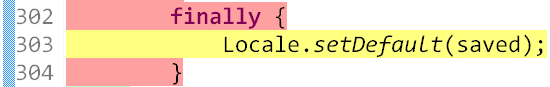
\includegraphics[width=2.5in]{Chapter-4/figs/finally-block}
	\caption{A notification from EclEmma regarding \texttt{finally} coverage (ECL5).}
	\label{fig:finally}
\end{figure}


Visual communication mismatches occurred when there was a mismatch between how the participant would communicate with other developers about the notifications and the visual elements used by the notifications.
For these challenges, it was clear there was a mismatch between what participants expected and what the tool presented them with, but there was no indication by participants of what specifically caused the mismatch.

For fourteen participants, EclEmma's attempts to communicate \texttt{finally} block coverage in ECL5 (Figure~\ref{fig:finally}) failed because it was not obvious, based on their mental model of how \texttt{finally} blocks work, how a \texttt{finally} block can be missed or the code inside a \texttt{finally} block could be partially covered. For example, \professional{P24} had expectations regarding how EclEmma might communicate coverage of a \texttt{finally} based on prior experience with the construct that suggests it always executes. Rather than exploring more, \professional{P24} noted he did not understand the way the tool communicated. 

Seven participants had expectations regarding how \texttt{try} blocks work that did not match how EclEmma reported \texttt{try} block coverage (ECL5).
For example, as \graduate{P23} sorted through the notifications in ECL5, he wanted to know which line failed to cause the \texttt{try} block to not execute.
Attempting to interpret the notification, he stated:

\begin{quote}
	\textit{In order for the \texttt{catch} statement to be activated I would imagine that this code had at least been evaluated.}
\end{quote}

\noindent
His expectation, based on his knowledge of the code construct, was that if the \texttt{try} did not execute, there was a line of code at fault. However, contrary to his expectations, EclEmma highlights the entire \texttt{try} block red if an exception is thrown, which makes it unclear whether the \texttt{try} executed at all, and if it did, where an exception was thrown.

Five participants got confused by EclEmma's lack of textual information.
Participants probably noticed this because both FindBugs and the compiler provide supplemental textual information when markers, similar to the ones provided by EclEmma, are clicked; in fact, markers and notifications from other tools within EclEmma's interface sometimes distracted participants looking for information regarding code coverage.
As \professional{P4} accessed the information provided by notifications in ECL6, he noticed and explored the availability of multiple markers that provided information. Some of these markers came from other tools; none provided \professional{P4} with ``any details about the coverage part,'' so he was not sure why they were present.

%These expectation mismatch challenges are general and focus on visual communication. Participants also encountered related, but more specific knowledge expectation mismatch challenges.


\subsubsection{Consistent Communication Mismatches}\label{subsec:inconsistent}
% challenges caused by tool communicating similar problems differently
Consistent communication mismatches occurred when there was a mismatch between the consistency expected by the participant and the inconsistencies in how the notifications communicated similar problems. 
Prior research suggests that within-tool-consistency is an important factor for developers when interpreting and addressing compiler messages~\cite{Traver:2010:Messages}.
The results in this category suggest that experiences affect perception of consistency and that this phenomena generalizes to visually-enriched notifications in other types of  tools.

Five participants encountered challenges caused by inconsistencies in how EclEmma reports coverage on branching structures. Under the assumption that yellow highlighting was accompanied by a textual description (i.e. 1 of 2 branches missed), participants often struggled to interpret notifications like the one in Figure~\ref{fig:finally}. \undergraduate{P6}, among others, spent a significant amount of time during her session trying to interpret the notifications in ECL5. When she realized that there were no markers available to better explain partial coverage inside a \texttt{finally} block, she began looking at the other similar notifications in ECL5. When she realized that none of the other notifications had what she was looking for, she summarized why she was struggling, stating ``I'm not sure what the other option could be\ldots it doesn't have the little yellow diamond on it.''

Six participants noticed inconsistencies in how EclEmma reported coverage on non-branching code structures. Five of the six encountered challenges interpreting notifications on methods and constructors. 
EclEmma highlights the constructor signatures to indicate a missed constructor, however, does not highlight a method signature when it is not executed. 
For example, during \professional{P14}'s session, he did a lot of back and forth between EclEmma tasks to compare notifications. As he tried to interpret the notifications in ECL3, he reflected on and revisited ECL1 and ECL2, where he recalled there being class, method, and constructor coverage. He remembered the inconsistencies with how ECL1 and ECL2 communicated coverage on these constructs and found it to be confusing. Therefore, he could not give a definite interpretation of any of the three. 

\subsubsection{Familiar Communication Mismatches}\label{subsec:intuitive}
% challenges caused by unintuitive communication; participants explicitly noted the notifications as being unintuitive
Familiar communication mismatches occurred when there was a mismatch between participant familiarity with the methods a notification uses to communicate about programming concepts and the methods the notification used to communicate about programming concepts When participants encountered these challenges, they often noted lack of familiarity or the inability to easily recognize the problem.
%color representations - P12, P15, P18, P21, and P24
Participants that noticed unintuitive communication techniques found some for all tools. The majority of participants (five of eleven) stated that EclEmma's dominant use of color to communicate code coverage was not intuitive. For example, participants did find it intuitive to use yellow for partial coverage in notifications like the ones in ECL3, ECL5, and ECL6. 
The common problem with the other tools involved association of the notification to the root cause and unintuitive fix descriptions.

\subsection{Member Check}
To assess the validity of how I interpreted the data, and the experiences developers have when interpreting tool notifications, we conducted a member check. Of the seven responses received, two developers agreed with these findings and five strongly agreed. Many found the report ``interesting,'' some noting that although they may not have experienced all of the challenges during the study, they can recall previously encountering such challenges. When asked which challenges they can relate to the most in their experiences with tools, the most common choice was Problem Resolution Gaps (5). The second most common responses (4) include Notification Experience Gaps and Information Salience Mismatches, followed by the third most common responses (3) of Conceptual Knowledge Gaps, Visual Communication Mismatches, and Familiar Communication Mismatches.

\section{From Theory to Practice}
Current tools do not support developer knowledge gaps (Section~\ref{subsec:gaps}) and sometimes conflicts with existing developer knowledge (Section~\ref{subsec:mismatch}).
In this section, I discuss several implications of the findings from this study.

\subsection{Filling Developer Knowledge Gaps}
Despite the experience of some participants, every participant encountered at least one notification they did not understand. 
FindBugs, the Eclipse Java Compiler, and EclEmma attempt to fill knowledge gaps to different degrees and in different ways. FindBugs sometimes provides definitions, examples, and fix suggestions. The compiler provides tooltip descriptions and often an automatic quick fix that developers can apply to learn about notification resolution. EclEmma sometimes provides tooltips to help developers fill knowledge gaps concerning low test coverage.

One straightforward solution is for tools to provide more information to developers to help fill knowledge gaps. For example, for developers that struggled with \texttt{finally} block coverage in ECL5, it may have been helpful if the tool provided information regarding \texttt{finally} block coverage in EclEmma. Or, for developers who did not know what synchronization is, it may have been helpful to provide a definition or code example of what it means to correctly synchronize an object or method.

Findings from this study suggest tools can fill developer knowledge gaps by consistently providing information about the options for fixing a notification (Section~\ref{subsec:resolution}) and reasoning for resolution (Section~\ref{subsec:rationale}). The Eclipse compiler makes a consistent effort to provide fix information, however, it does not make an explicit effort to assist developers with deciding the \textit{best} fix their code nor does it provide rationale for resolution. Mu{\c{s}}lu and colleagues provided one potential solution for compiler notifications with \textsc{Quick Fix Scout}~\cite{Mucslu:2012:Speculative}. Although this approach could be applied to other tools that offer quick fixes, like FindBugs, \textsc{Quick Fix Scout} prioritizes and rationalizes based on one criteria: the number of new notifications introduced by applying the fix. However, other criteria, 
such as whether the fix uses familiar APIs, may also improve the usability of program analysis notifications.


\subsection{Matching Developer Expectations}
Developer expectations can have an effect on their ability to interpret notification messages (Section~\ref{subsec:mismatch}). 
I propose that tools can improve how they communicate to developers if they are able to ascertain developers' knowledge and experiences, which inform their expectations~\cite{dean1982computer}.
For each notification in this study, some developers could interpret the notification and others could not. Therefore, it may be that providing every developer with more information is not the best way to support developers' understanding of tool notifications.

If a tool could know its user's familiarity, or unfamiliarity, with the notifications it provides, or the concepts in those notifications, the tool could determine how to adapt its notifications to better fit the user's expectations.
However, tools cannot acquire the knowledge required to build these constructs on their own. 

% adaptations based on concept, notification, and tool experience; possibly even other things (i.e. academic vs. non-academic training - P20 as example)                    
What if it was possible to determine the best links to external resources for a developer based on the concepts relevant to the notification the developer knows the least about?
Or display information based on what is most needed or used by the developer?
One solution, modeled after intelligent tutoring systems (ITS)~\cite{tutoringsys}, would be for tools to use developer knowledge, in the form of their experiences, as a factor when determining the information necessary for a developer to interpret a given notification~\cite{johnson2015bespoke}.

Imagine two developers, D1 and D2; D1 frequently develops in multi-threaded environments while another, D2, is new to multi-threading. 
For multi-threading experts, like D1, extra information regarding terms and fundamental concepts, such as lazy initialization, may not be necessary. 
It may be enough to notify her and provide quick access to a suggestion or example for resolving the problem; it may even be distracting having other information available she likely does not need. 
For multi-threading novices, like D2, all the information provided could be of use; such novices may need even more information.

ITS create student models based on assessments; we imagine IDEs could construct a model of a
developer's experience by observing their use of language features, tools, and libraries in the code they write.
This is similar to the design of other kinds of notifications~\cite{mccrickard2003attuning, sow2005tasks, Zhang:2005} 
and aligns with research on recommendation systems that suggests data mining and 
other knowledge inference techniques can help provide previously-unknown 
information for task completion~\cite{robillard2014recommendation}.
%TODO this could use an example
There may be factors other than their coding experience to consider for accurate models. Other data we can collect include notifications the developer has resolved or portions of the notification text frequently visited or used by the developer.

In order to adapt tool notifications to a given developer's knowledge, there needs to be some notion of how much the developer knows about the concepts in the notification. For the remainder of this document, I use concept to mean programming concepts. I chose to focus on programming concepts because the findings from this study, and existing research conducted by Smith and colleagues, suggests understanding programming concepts affects developers' ability to understand and resolve notifications~\cite{smith2015questions}. Borrowing from education research and using developer experiences as a concrete representation of knowledge, the remainder of this thesis evaluates the possibility to ascertain and approximately predict developer knowledge of programming concepts.

\chapter{Assessing Developer Knowledge}
\label{chap:assess}

To create any kind of model, I need a dependent variable and one or more independent variables that could be used to predict the value of the dependent variable. Since I want to build models that predict knowledge, my dependent variable has to be some measure of developer concept knowledge.
Borrowing from existing computer science education research, I developed concept inventories for knowledge assessment. 

A concept inventory, or CI for short, is a validated assessment that uses multiple-choice questions to aid instructors in assessing student understanding of relevant domain or course concepts, while also identifying student misconceptions~\cite{evans2003progress}. Concept inventories can cover any range of concepts and originated in the field of physics with the Force Concept Inventory~\cite{hestenes1992force}. There are guidelines for creating concept inventories, such as avoiding catch-all options like ``All of the above'' and using empirical methods to validate and improve inventory questions and items. Most often in the natural sciences and engineering, inventories assess breadth of knowledge across the subject or course of interest~\cite{evans2003progress}. In Computer Science, for example, a range of CS1 concepts can be represented in a given concept inventory~\cite{tew2010developing}.

% TODO does this need to go to RW?	
Borrowing from concept inventories used in other STEM fields, CS Education researchers and instructors have developed various concept inventories for assessing students' knowledge of introductory Computer Science concepts\cite{almstrum2006concept, krone2010reasoning,tew2010assessing}. Almstrum and colleagues created concept inventories to assess student knowledge of concepts taught in a discrete mathematics course~\cite{almstrum2006concept}. 
Tew and Guzdial developed a concept inventory for assessing students' knowledge of CS1 concepts in introductory Computer Science courses~\cite{tew2010assessing, tew2010developing}. These inventories used textbooks and experts to create test specifications that they then validated using empirical methods, such have CS Education experts review the specification. Fundamental concepts included on their concept inventory include object-oriented programming and control structures. Similar to other Computer Science concept inventories, Tew and Guzdial's CS1 concept inventory assess breadth of knowledge. 
	
Related to the concept inventories developed by Tew and Guzdial, Zingaro and colleagues developed ConcepTests~\cite{zingaro2010experience} used in to monitor and assess student understanding of computer science concepts as they were taught. Similar to my concept inventories, these ConcepTests focus on one specific concept at a time except with the goal of encouraging and implementing peer instruction (PI). In contrast, Zingaro and colleagues do not use the validated steps for creating a concept inventory to create their assessments.
	
Also closely related to my approach and the goal of my inventories is the work of Karpierz and Wolfman, who designed a variety of multiple choice questions for concept inventories on binary search trees and hash tables~\cite{Karpierz2014Misconception}. Rather than focusing on various Computer Science concepts at once, they focus on developing questions to assess specifically binary search trees and hash tables. Contrary to our approach, they only deployed their concept inventory once -- during the last lecture of the course. This eliminates the possibility of comparing how much students knew before taking the course and how much they know now, which I assess with my concept inventories.
	
Although these concept inventories have been proven useful in various contexts, some instructors believe, and research suggests, we should be moving away from textbook-driven lessons and assessments, and employ more focused efforts to monitor student learning and understanding~\cite{pellegrino2001knowing, ghezzi2005challenges, wohlin1999achieving}. This work builds on existing work by adapting current methods used to develop concept inventories by 1) assessing depth of knowledge regarding a single programming concept, 2) using language specification, tutorials, and other technical documents to create the content of the concept inventories, and 3)incorporating practical software engineering concepts, such as tool use.

\section{Modified Concept Inventories}

Traditionally, concept inventories are used to  assess conceptual knowledge across concepts; in Computer Science, the target audience is typically CS1 students~\cite{tew2010developing,kaczmarczyk2010identifying}. 
I wanted to evaluate the potential for a depth versus breadth approach to assessing conceptual knowledge, that incorporates software engineering concepts and practices, with the target audience being developers at any stage of expertise.
Therefore, I could not borrow directly from research that uses a breadth approach to create concept inventories that assess high level knowledge of concepts taught in an introductory course~\cite{tew2010assessing}. I extended existing concept inventory research~\cite{tew2010developing,nelson1967testing} by using the new Bloom's Taxonomy to create questions~\cite{scott2003bloom,thompson2008bloom, starr2008bloom}, subjective resources like language specifications to determine sub-concepts relevant to a single concept, and tool output, including compilation errors and warnings, to integrate practical applications of the programming concepts. The differences between my approach and existing approaches is highlighted in Table~\ref{table:diff}.
The final process we have developed for creating general knowledge programming concept inventories that assess depth of knowledge is as follows:

\begin{enumerate}
    \item Define Conceptual Content for Test Specification
    \item Build Bank of Test Questions
    \item Pilot Questions
    \item Establish Validity and Reliability
\end{enumerate}




	\begin{table}[ht]
		\centering
		\caption{Summary of the differences between my approach and existing approaches.}
		\label{table:diff}
		\rowcolors{2}{gray!25}{white}
		\begin{tabular}{lll}
			\toprule
		    \rowcolor{gray!50}
			& \multicolumn{1}{c}{\textbf{Existing CS Concept Inventories}}                                              & \multicolumn{1}{c}{\textbf{My Concept Inventories}}\\
			\midrule
			\textbf{\begin{tabular}[c]{@{}l@{}}Defining Concept \\Content  for \\ Test Specification\end{tabular}} & \begin{tabular}[c]{@{}l@{}}Textbooks; provide definitions to \\ CSEd experts for review \end{tabular}                                                   & \begin{tabular}[c]{@{}l@{}}language specifications, language \\ tutorials, and documentation\end{tabular}      \\
			\textbf{\begin{tabular}[c]{@{}l@{}}Build Bank of \\Test Questions \end{tabular}}                                                              & \begin{tabular}[c]{@{}l@{}}Three types of questions \\ (Definitional, Tracing, Code Completion)\end{tabular} & \begin{tabular}[c]{@{}l@{}}Six types of questions (Bloom's \\ Taxonomy), tool output, compilation\end{tabular} \\
			\textbf{Pilot Questions}                                                                            & Collect data for later analysis                                                                              & \begin{tabular}[c]{@{}l@{}}Iteratively conduct think aloud\\ and modify \end{tabular}                                                                     \\
			\textbf{\begin{tabular}[c]{@{}l@{}}Establish Validity \\ \& Reliability \end{tabular} }                                                         & Empirical analysis of responses                                                                              & Item and distractor analysis\\  
			\bottomrule
		\end{tabular}
	\end{table}

\section{Defining Conceptual Content}

A test specification is a way of formally outlining what will be on the test without having to write any of the questions~\cite{tew2010developing}. Once a decision has been made concerning the programming language and concept(s) of interest, rather than using expert review to determine appropriate sub-concepts concepts, use a more objective, practical approach. This is achieved by using language specifications, tutorials, and other documentation surrounding that concept. This is an iterative process meant to increase the depth of assessment on the concept and related sub-concepts.

% To better understand how we constructed and validated our concept inventories, let us consider our most recent concept inventories on generics and exception handling.
To determine the conceptual content for each concept inventory, I identified key concepts from the most up to date the Java Language Specification (JLS)~\cite{Gosling:1996:JLS:560667} and the Oracle Java Concept Tutorials\footnote{\url{http://docs.oracle.com/javase/tutorial/java/generics/}} on the concept of interest. The Oracle Java Tutorial was most useful for finding and mapping the relationships between concepts and ancestor concepts; if Lesson X built on top of Lesson Y, we consider Lesson Y an ancestor of Lesson X. For example, based on the generics tutorial, we labeled Upper Bounded Wildcards as an ancestor concept to Wildcards. 

	\begin{figure*}[ht]
		\centering
		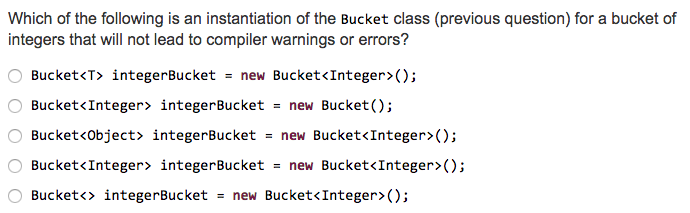
\includegraphics[width=4in]{Chapter-5/figs/generics-Q2.png}
		\caption{Question assessing ability to evaluate generic type instantiation.\label{fig:Q2}}
	\end{figure*}	
	
Once I had a list of concepts and sub-concepts, I created questions to assess the various concepts, mapping each question to at least one level of Bloom's Taxonomy. I used examples found in the language specifications and tutorials, along with relevant tool output, to create questions for each inventory. For example, the item shown in Figure~\ref{fig:Q2} is a question on the generics concept inventory that asks a question to determine the student's ability to \textbf{evaluate} a problem pertaining to instantiating a generic type (\texttt{Bucket}). According to the new Bloom's Taxonomy, evaluation includes Checking and Critiquing, which involves students making decisions based on criteria. In terms of Computer Science, prior works suggests this can be done by, for example, assessing students' ability to determine if a piece of code satisfies requirements (i.e. compilation) or critiquing the quality of the code based on known standards~\cite{thompson2008bloom}.

\section{Building A Bank of Questions}

Based on existing concept inventory research, the questions on concept inventories should be multiple choice and all questions should have the same number of items to choose from~\cite{tew2010developing}; typically there are 4--5 items. Existing work also recommends avoiding catch-all items such as ``All of the above'' and ``None of the above''~\cite{tew2010developing}. While one of the items should be the best right answer, other options, known as distractors, should be plausible permutations that are believable but incorrect. 

Next, using the revised Bloom's Taxonomy, which is the most up to date version of the taxonomy, is to derive a bank of test questions. Using Bloom's Taxonomy increases assurance that the questions assess different levels of understanding, which helps assess mastery of a concept~\cite{scott2003bloom, thompson2008bloom}. Each question should map to at least one level of Bloom's Taxonomy~\cite{starr2008bloom,khairuddin2008application}; rigor increases at each level. I found it helpful to compare the kinds of questions asked at each level of Bloom's Taxonomy with the questions in the bank to be used. I believe it is more effective if each level of Bloom's Taxonomy is represented in the bank of questions at least once rather than only focusing on certain levels of the Taxonomy~\cite{scott2003bloom}. 
To further incorporate practical aspects of software engineering, for each inventory, create questions that ask about code compilation, writing quality code, and resolving tool output. 
% Instructors can use languages and tools of their preference for creating these questions; we believe it is ideal if they are tools instructors plans to or already has introduced to students.

\section{Think Aloud Pilots}
Once there is a bank of questions, the next step is to pilot the questions. The goal of this pilot is to determine if there are any obvious ambiguities in the questions or options. Consistent with Parker and colleagues~\cite{parker2016replication}, we recommend a think-aloud activity where students take each concept inventory and report questions or items that stand out as confusing and why. As participants note ambiguous words or phrases used in the questions or items, immediately make modifications before having any others pilot the inventory. When observing the scores, if all the scores are really high, or really low, this might suggest an assessment that is too difficult or too easy~\cite{nelson1967testing}, which would require revisiting and revising the questions or items. To ensure items contribute to overall effectiveness, use statistical methods to validate the concept inventories.

I piloted my concept inventories with undergraduate and graduate students. For each student, I asked them to take the inventory as they normally would and let us know when one of the following occurs:
	
	\begin{itemize}
		\item They came across a question where the phrasing did not make sense or was unclear.
		\item The came across an option for a question that did not make sense or was unclear.
		\item They encountered a question where they believed more than one option could be correct.
		\item They encountered a question where none of the options appear to be correct.
		\item They noticed any typos or discrepancies in the questions, options, or code examples.
	\end{itemize}
	
I made note during this process of any issues participants encountered, asked them to explain that difficulty, and how it could be improved. Once that participant finished the concept inventory, I immediately integrated the necessary changes into the concept inventory. I iterated this process with all pilot participants.

\section{Concept Inventory Validation}

Validation of an assessment tool can be done in a variety of ways.
To test the validity of my concept inventories and the items on each, I conducted \textit{item analysis} and \textit{distractor analysis} using R statistical software~\cite{boopathiraj2013analysis, RSoftware}. 
I ran these analyses based on data gathered from a different sample than the group used for the initial think aloud pilot. 

\subsection{Item Analysis}
The most common form of validation is item analysis~\cite{gorsuch1997exploratory}.
Item analysis determines if inventory items are valid methods of assessment; most often, the item difficulty and discrimination index are used to assess test quality~\cite{boopathiraj2013analysis}. For item difficulty, an item is considered too easy if its item difficulty value (Item Difficulty, Table~\ref{table:items}) is 0.95--1.00 and too difficult if it is less than 0.20. An optimal question has an item difficulty value of 0.50, however, the primary goal is to not have any questions, based on the item difficulty value, that are too hard or too easy. 

A question is considered satisfactory if the discrimination index (Point Biserial, Table~\ref{table:items}) is greater than 0.20. The difficulty and point biserial values can be positive or negative; a negative value suggests an item should be removed or replaced.
The threshold value (Item Threshold, Table~\ref{table:items}) provides the same information as the difficulty value; the lower the value, the easier the question. 
The biserial value (Biserial, Table~\ref{table:items} describes the degree of relationship between two interval scales. For the type of validation needed for the inventories, the threshold and biserial are not relevant.


To clarify the validation process, I present item analysis results from the exception handling concept inventory as an example. This was the concept inventory that underwent the most change as a result of this process. Table~\ref{table:items} shows the item analysis output from the initial set of exceptions questions put in thee inventory and piloted with 10 students and developers. I wanted to include developers with industry experience to evaluate the more advanced questions on the inventory. I performed pilots with students and those with industry experience to evaluate how well the concept inventory assessed different levels of knowledge regarding exception handling. Based on the output, one of the questions removed was item 3, which is shown in Figure~\ref{fig:item3}. The discrimination index for this item (-0.024) is too low, which means that it was not a good item for discriminating between students who are knowledgeable in exception handling and those who are not. Based on these numbers, I also removed items 4, 8, and 9.

	\begin{table}[]
		\centering
		\caption{Exception handling concept inventory item analysis results}
		\label{table:items}
		\begin{tabular}{lllll}
			\toprule
			& \multicolumn{1}{c}{\textbf{\begin{tabular}[c]{@{}c@{}}Item \\ Difficulty\end{tabular}}} & \multicolumn{1}{c}{\textbf{\begin{tabular}[c]{@{}c@{}}Item \\ Threshold\end{tabular}}} & \multicolumn{1}{c}{\textbf{Point Biserial}} & \multicolumn{1}{c}{\textbf{Biserial}} \\
			\midrule
			\textbf{Item 1}  & 0.917                                                                                   & -1.383                                                                                 & 0.271                                       & 0.489                                 \\
			\textbf{Item 2}  & 0.333                                                                                   & 0.431                                                                                  & 0.098                                       & 0.127                                 \\
			\textbf{Item 3}  & 0.667                                                                                   & -0.431                                                                                 & -0.024                                      & -0.032                                \\
			\textbf{Item 4}  & 0.917                                                                                   & -1.383                                                                                 & 0.271                                       & 0.489                                 \\
			\textbf{Item 5}  & 0.500                                                                                   & 0.000                                                                                  & 0.553                                       & 0.694                                 \\
			\textbf{Item 6}  & 0.500                                                                                   & 0.000                                                                                  & 0.484                                       & 0.607                                 \\
			\textbf{Item 7}  & 0.583                                                                                   & -0.210                                                                                 & 0.690                                       & 0.872                                 \\
			\textbf{Item 8}  & 1.000                                                                                   & -Inf                                                                                   & N/A                                         & N/A                                   \\
			\textbf{Item 9}  & 0.500                                                                                   & 0.000                                                                                  & 0.899                                       & 1.000                                 \\
			\textbf{Item 10} & 0.833                                                                                   & -0.967                                                                                 & 0.495                                       & 0.738                                 \\
			\textbf{Item 11} & 0.500                                                                                   & 0.000                                                                                  & 0.899                                       & 1.000                                 \\
			\textbf{Item 12} & 0.667                                                                                   & -0.431                                                                                 & 0.489                                       & 0.634                                 \\
			\textbf{Item 13} & 0.583                                                                                   & -0.210                                                                                 & 0.690                                       & 0.872                                 \\
			\textbf{Item 14} & 0.667                                                                                   & -0.431                                                                                 & 0.342                                       & 0.444\\                                
			\bottomrule
		\end{tabular}
	\end{table}
	
	
	\begin{figure}[]
		\centering
		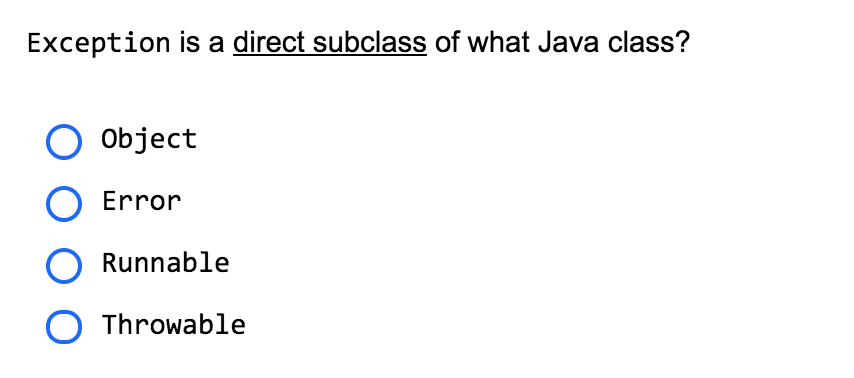
\includegraphics[width=3in]{Chapter-5/figs/item3.png}
		\caption{Item removed from original concept inventory. \label{fig:item3}}
	\end{figure}

\subsection{Distractor Analysis}
I also recommend distractor analysis to evaluate the changes made during the think-aloud piloting. Distractor analysis determines if the options provided for a given question are fair and if the incorrect options contribute to the quality of the inventory. If the incorrect options are nonsensical or would make no sense as the answer, this takes away from the quality of the concept inventory. For example, if the only item that makes sense is the correct response, the chances that students can guess the right response as opposed to knowing the right response is increased.

The goal is for there to be no distractors that are not being selected and for the high performers (middle to upper range) to most often select the correct response. Because this was the case in the data for all the inventories, I kept all response options for each inventory item.\footnote{The final version of the concept inventories can be found at the following urls: \url{http://go.ncsu.edu/null}(null object dereferencing), \url{http://go.ncsu.edu/generics}(generics), \url{http://go.ncsu.edu/exceptions}(exception handling).}
% TODO footnote ==> appendix?
As with previous work, because establishing reliability for one inventory requires data from multiple trials, it may be better to save exploring reliability for future analysis~\cite{tew2010developing,tew2010assessing}.


	
% TODO talk about applications for my inventories?? stuff in paper = education only :/ 
% TODO talk about industry and classroom applications -- end with how I'm using them?


\section{Limitations \& Challenges}\label{sec:limits}

Despite the possibilities for our approach for creating and deploying these concept inventories, there are some limitations. 

\begin{itemize}
	\item \textbf{Upfront time commitment.} Although there is value inside and outside the classroom in the process we proposed for depth of knowledge assessment, there is an upfront time cost involved in creating an inventory using our process. In our experience, after creating the first couple of inventories, especially with the up front cost of understanding how to conduct item analysis and what the results mean, the amount of time it takes to create new inventories decreases.
	\item \textbf{Lack of automation for individual response assessment.} Currently, to our knowledge, there is no automated way to observe individual student responses and changes over time, outside of item analysis. Item analysis, which we performed on pilot data from our concept inventories, provide some insights into the effectiveness of each item on the evaluation. However, it does not ease the process of determining which concepts need more attention in class or lab which is one of the potential uses for our inventories.
	\item \textbf{Guaranteeing student's responses are their own.} Even though we did not deploy our concept inventories for a grade, it is still possible that students used outside sources, or even each other, to help determine answers on the inventory. There is no sure way to guarantee students are not using outside resources. However, we attempted to mitigate this limitation by only allowing so much time for taking the inventory and making it an in class exercise rather than a homework assignment.
	\item \textbf{Keeping concept inventories up to date.} Depending on the language concepts are being taught in, there may be a need to periodically re-assess the material on the inventory for updating. So far, we have not had to make any updates however generics and exception handling are great examples of language features that has evolved since it has been out. Because our concept inventories aim to achieve depth of knowledge assessment, it is important that all relevant sub-concepts are represented in the inventory.
	\item \textbf{Lack of student participation.} Because the exercise is not graded, and in short our concept inventories are specialized quizzes, students may not be enthusiastic about having to take them. The hope is that, however, students who are genuinely interested in the coursework and progressing will take the inventories seriously whether they are enthusiastic about it or not.
	\item \textbf{Deploying the same concept inventory twice.} When deploying our concept inventories, we provided students with the same inventory as their pre- and post-evaluation and, if interested, they could continue past the end of the inventory to see which responses they got correct or incorrect. This introduces the potential that students are learning from the concept inventory rather than the lectures. Although we are unsure of how many students looked at what they got right and wrong, we argue that it is not a disadvantage for students to learn from the concept inventory. Because we use very few definition questions on our inventories, students are given access to practical problems and solutions that can benefit them in the future. 
\end{itemize}
\chapter{Developer Knowledge Classification}
\label{chap:experience}

In the previous chapters, I proposed that communication between notifications and developers could be improved if the information provided by notifications could adapt to the developer based on the developer's knowledge. 	
For it to be possible to adapt the information provided by notifications, tools need a way of knowing what concepts the developer knows and does not know. Furthermore, tools also need a way of knowing how well developers know these concepts. 	

In Chapter~\ref{chap:assess}, I outlined an approach for assessing developer knowledge of programming concepts. However, it is impractical and possibly infeasible to create a concept inventory for every programming concept and then ask developers to take that inventory before or while using a tool. It would be more practical and feasible if there was a way to use information already available to represent developer knowledge. I propose using developer experiences, in the form of the code they have written, to represent their knowledge of programming concepts. For the remainder of this document, I will refer to knowledge of programming concepts as \textit{conceptual knowledge}.  

Perception of any information provided to a developer is affected by that developer's knowledge and experiences; as a software developer, much of the knowledge accrued comes from experiences writing and modifying source code~\cite{Canas:1994:Mental,raju1995differential,fritz2010degree,argote2011organizational}.

However, currently tools have no way of assessing anything about the developer's knowledge.
Existing work in the area of source code mining has focused on measuring and predicting functional and non-functional properties of software~\cite{heckman2009model,menzies2007data,haapio2011exploring}. 
Contrary to much of the work in this area, I used source code mining to predict developer knowledge of programming concepts.

Based on previous research that suggests we can use source code as an indicator of how much a developer knows about a codebase~\cite{fritz2010degree}, I believe source code can also be an indicator of what developers know about programming.
Therefore, I designed a study to answer the following research questions:

\begin{itemize}
	\item [RQ\textsubscript{1}]: \textit{Is source code a good predictor of how much developers know about programming concepts?}
	\item [RQ\textsubscript{2}]: \textit{Does concept-specific source code increase the ability to classify how much developers know about programming concepts in comparison to a naive model?}
\end{itemize}

To answer these questions, I built and evaluated models that classify developers' conceptual knowledge. To determine if source code is a good predictor, I compared these models to random chance and a naive model that uses all the source code written by the developer (LOC).
The assumption is that if my models can classify developers with greater than 50\% accuracy, they perform better than random chance.
I collected source code relevant to the Java programming concepts of variables, exception handling, and generics from 19, 35, and 23 developers, respectively. 
I distributed the concept inventories described in Chapter~\ref{chap:assess} to validate conceptual knowledge for each model. 
I trained each model using source code the developers wrote pertaining to each programming concept, or \textit{concept-specific code}, in public GitHub repositories. 
I used unsupervised learning to determine a model that classifies developers based on their conceptual knowledge. 
Specifically, I calculated model metrics, such as precision, recall, and false positive rate, to determine and compare model performance.

% TODO make sure each chapter has contribution(s) listed -- a summary like this at the end of each chapter intro would be nice	
The contribution of this chapter is a validated approach and set of models for predicting developer conceptual knowledge using public developer source code contributions. For RQ\textsubscript{1}, I found that models using source code outperformed a model that randomly assigns developers' expertise. For RQ\textsubscript{2}, I found that concept-specific models outperformed models that attempt to assign expertise based on total lines of code (LOC) written.

\section{Knowledge Acquisition}
% TODO do I need to expand on this more?
According to existing research, we acquire knowledge through our experiences~\cite{argote2011organizational}. For example, a chef's knowledge regarding recipes, best practices, and what tastes good comes from their experiences cooking in both professional and informal settings. Just as a chef gains knowledge from her experiences, as do other professions. Software development is no exclusion.

Much of what software developers do involves looking at, writing, or modifying source code. 
There are a variety of other experiences that come with being a software developer. However, for scoping and proof-of-concept purposes, I focus on the primary task of software development which is writing code.
In the following section, I discuss how I used concept inventories and developer source code contributions to classify developer based on their conceptual knowledge.

\section{Knowledge Classification}

To determine the ability to use developer source contributions to predict developer knowledge, I used concept inventories to validate developer knowledge and source code contributions on GitHub to predict validated knowledge classifications.
To explain the process used to validate and predict developer knowledge, I will use a hypothetical developer Gabrielle and her experiences writing code as an example.

\subsection{Knowledge Validation}

To determine ground-truth developer knowledge for the models, I borrowed from computer science education literature and developed a set of concept inventories~\cite{tew2010assessing}.
The process for creating and validating these inventories is discussed in detail in Chapter~\ref{chap:assess}.
The scores from the concept inventories provide data that I used to provide an independent attribute for each model. 

\subsection{Knowledge Prediction}
% process for predicting knowledge
The goal of this study was to determine the possibility of using developer source code contributions to predict how much they know about programming concepts in their tool notifications.
Using developer source code, along with their concept inventory scores and the independent attributes, I used unsupervised learning to determine the relationship between the two.

\begin{figure} [ht]
	\centering
	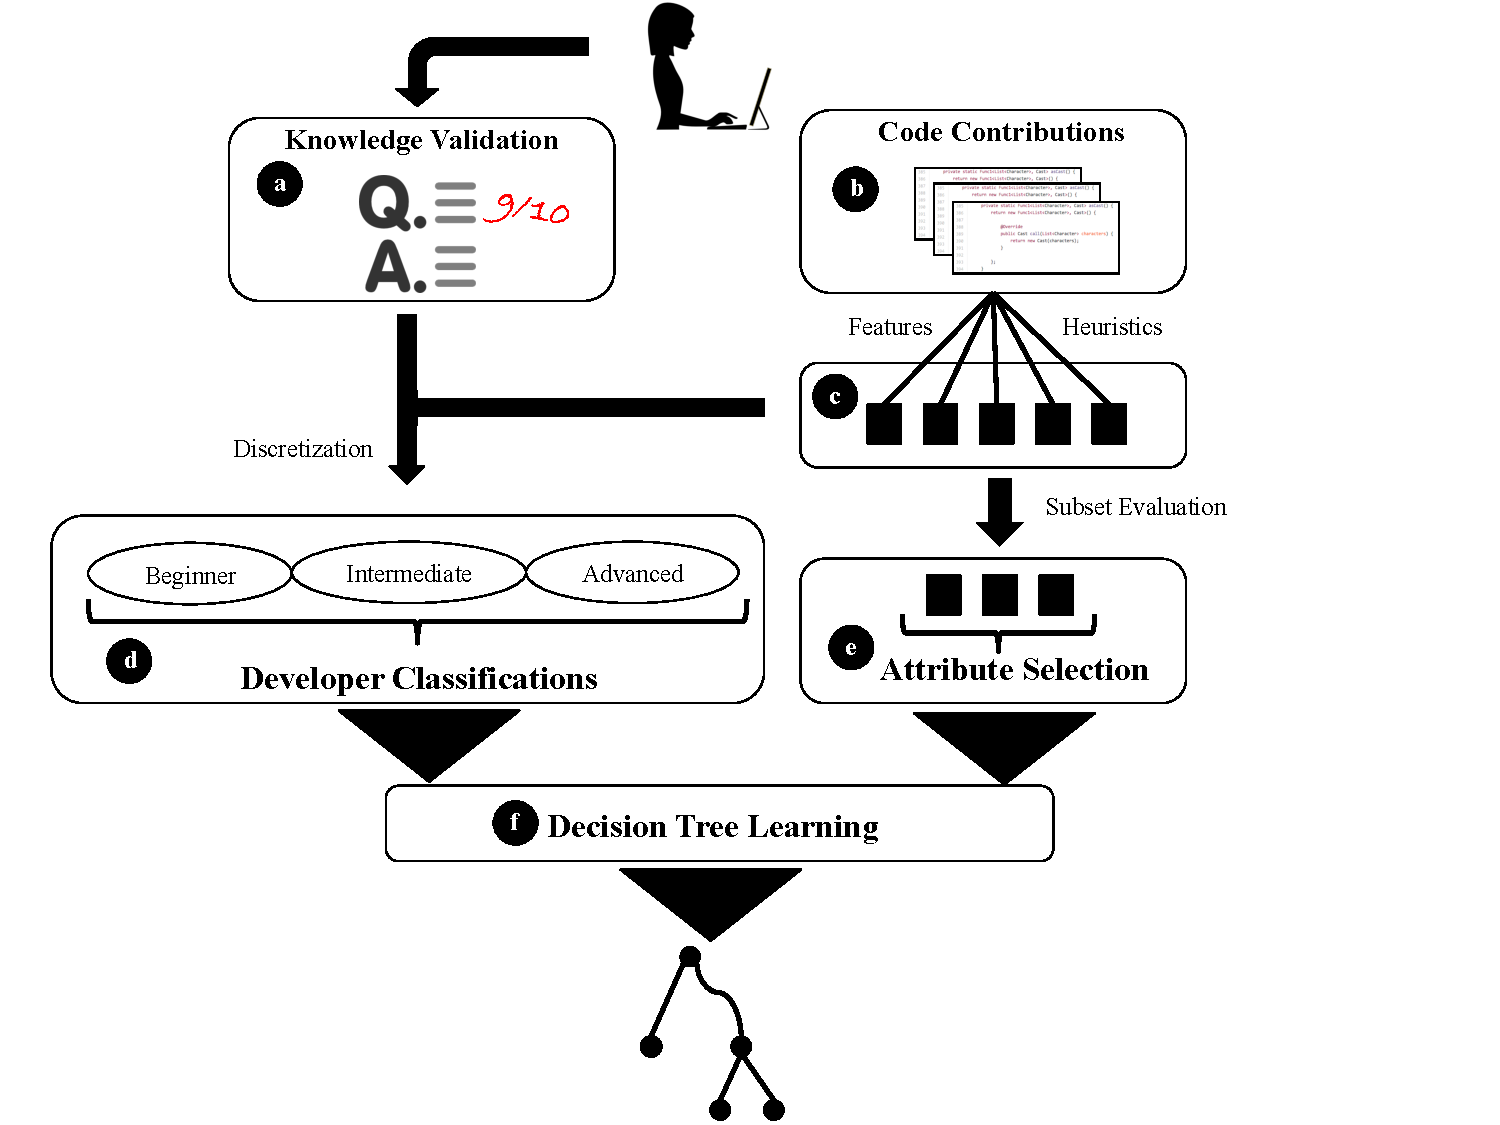
\includegraphics[width=4.5in]{Chapter-6/figs/approach-fig.pdf}
	\caption{An overview of my approach.}
	\label{fig:approach}
\end{figure}

\subsubsection*{Source Code Contributions} \label{subsec:code}

To determine the dependent attributes for each model, and answer \textbf{RQ\textsubscript{1}}, I analyzed developers' public repositories for code contributions and assigned them to developers using version control (Figure~\ref{fig:approach}b).

Consider the code in Figure~\ref{fig:code}, which is a portion of code from the JUnit4\footnote{\url{http://junit.org/junit4/}} repository. Gabrielle contributes to this repository often, which provides rich data regarding her experiences with programming concepts. I analyzed developer source code using the Eclipse JDT ASTParser~\cite{eclipseASTParser}. Analyzing code statically with the ASTParser detects the presence of concept-specific code. However, it cannot tell us who contributed that code. In order to predict individual developer knowledge, we need to be able to identify that developer's code contributions.

Therefore, I used code bases in repositories so we could determine what developer made what contribution via the commit history. Since I chose the versioning platform Git,\footnote{\url{https://git-scm.com/}} I used JGit\footnote{\url{http://eclipse.org/jgit/}}, a Java library that allows for manipulation of Git repositories via Java code. Also,  next to SVN, Git is one of the most popular versioning softwares in use today.\footnote{\url{http://www.openhub.net/repositories/compare}}  Along with using ASTParser, I used JGit to analyze for individual developer code contributions. 

Previous research suggests time may play a factor in how predictive code contributions can be~\cite{johnson2015bespoke}, therefore I also used JGit to detect when the most recent contribution of each type of concept usage was made.
We chose to use GitHub, a social coding site where developers can create and maintain Git repositories,\footnote{\url{http://www.github.com}} as the source of data because GitHub stores Git repositories and many repositories on GitHub are public.
Once a plan was in place for analyzing developers repositories, to answer RQ\textsubscript{1}, I next identify source code that is directly related to the programming concepts of interest. 

\newcolumntype{g}{>{\columncolor{gray!40}}l}

\begin{table*}
    \centering
	\caption{Source Code Collected for Variables}
	\label{tab:var_code}
	\def\arraystretch{1.2}
	
	\begin{tabular}{ggg}
	    \toprule
		\rowcolor{white}
		\textbf{Source Code}                     & \textbf{Description}                                          & \textbf{Example}   
		\\
		\midrule
		\rowcolor{white}
		\textit{Primitive Types}        & \begin{tabular}[c]{@{}l@{}}data type is one of the most basic  \\Java data types (i.e. \texttt{int}) and store \\a value.\textbf{$\star\star$} (\textbf{D})\end{tabular}                                        & \small{\texttt{int a = 3;}}                                                                  \\
		\textit{Non-Primitive Types}    & \begin{tabular}[c]{@{}l@{}}data type is a reference data type \\and stores a reference to an object.\textbf{$\star$} (\textbf{D})\end{tabular}          & \small{\texttt{Object o = new Object();}}                                                    \\
		\rowcolor{white}
		\textit{Fields}                 & \begin{tabular}[c]{@{}l@{}}created to be accessed globally \\ by a class.\textbf{$\star$} (\textbf{D}) \end{tabular}                                                                               & \small{\texttt{public String s;}}                                                            \\
		
		\textit{Local Variables}        & \begin{tabular}[c]{@{}l@{}}created and assigned a value to be accessed \\locally by a method or construct.\textbf{$\star\star$} (\textbf{D}) \end{tabular}     & \small{\texttt{public String s = "hi";}}                                                     \\
		\rowcolor{white}
		\textit{Parameters}             & \begin{tabular}[c]{@{}l@{}}used as parameters to pass information \\into a method the developer created.\textbf{$\star\star\star$} (\textbf{D})\end{tabular}       & \small{\texttt{public void foo (String s)}}                                                  \\
		\textit{Public Variables}       & includes the public modifier.\textbf{$\star\star$} (\textbf{D})                                                                                              & \small{\texttt{public String s = "hi";} }                                                    \\
		\rowcolor{white}
        \textit{Private Variables}      & includes the private modifier.\textbf{$\star\star$} (\textbf{D})                                                                                              & \small{\texttt{private String s = "hi";}}                                               \\
		 \textit{Protected Variables}    & includes the protected modifier.\textbf{$\star\star\star$} (\textbf{D})                                                                                          & \small{\texttt{protected String s = "hi";}}                                                  \\
		\rowcolor{white}
		\textit{Static Variables}       & includes the static modifier.\textbf{$\star\star$} (\textbf{D})                                                                                              & \small{\texttt{static String s = "hi";}}                                              \\
		\textit{Final Variables}        & includes the final modifier.\textbf{$\star\star\star$} (\textbf{D})                                                                                                & \small{\texttt{final String s = "hi";}}                                               \\
		\rowcolor{white}
		\textit{Transient Variables}    & includes the transient modifier.\textbf{$\star\star\star$} (\textbf{D})                                                                                            & \small{\texttt{transient String s = "hi";}}                                           \\
		\textit{Volatile Variables}     & includes the volatile modifier.\textbf{$\star\star\star$} (\textbf{D})                                                                                           & \small{\texttt{volatile String s = "hi";}   } 
		\\
		\bottomrule
	\end{tabular}
	
\end{table*}

\begin{table*}
    \centering
	\caption{Source Code Collected for Exceptions}
	\label{tab:excep_code}
	\def\arraystretch{1.2}
	\begin{tabular}{ggg}
	\toprule
	\rowcolor{white}
		\textbf{Source Code}                     & \textbf{Description}                               & \textbf{Example}                                                                     \\
		\midrule
		\rowcolor{white}
		\textit{Throws Methods}         & \begin{tabular}[c]{@{}l@{}}method that throws an \\exception in the signature.\textbf{$\star$} (\textbf{U}) \end{tabular}                                & \begin{tabular}[c]{@{}l@{}}\small{\texttt{public void foo() }} \\\small{\texttt{throws IOException} }    \end{tabular}                                   \\
		\textit{Try Statements}         & non-empty try block.\textbf{$\star\star$} (\textbf{U})                                                                                                        & \small{\texttt{try \{ ... \}}}                                                               \\
		\rowcolor{white}
		\textit{Catch Blocks}           & non-empty catch block.\textbf{$\star$} (\textbf{U})                                                                                                      & \small{\texttt{catch (IOException e)\{...\}}}                                                \\
		\textit{Multi-Catch Blocks}     & \begin{tabular}[c]{@{}l@{}}non-empty catch block \\that use the  multi-catch \\operator ( $\vert$ ).\textbf{$\star\star\star$} (\textbf{U})\end{tabular}             & \begin{tabular}[c]{@{}l@{}}\small{\texttt{catch (IOException }} \\\small{\texttt{| SecurityException e) }}\end{tabular}
		\\
		\rowcolor{white}
		\textit{Try-With-Resources}     & \begin{tabular}[c]{@{}l@{}}non-empty try block that \\uses the try-with-resources \\feature.\textbf{$\star\star\star$} (\textbf{U})\end{tabular}                    & \begin{tabular}[c]{@{}l@{}}\small{\texttt{try (BufferedReader br =}} \\ \small{\texttt{new BufferedReader())}} \end{tabular}          
		\\
		\textit{Finally Blocks}         & non-empty finally block.\textbf{$\star\star\star$} (\textbf{U})                                                                                                 &  \small{\texttt{finally \{...\}}}                                                                           \\
	    \rowcolor{white}
	    \textit{Throw Statements}       & \begin{tabular}[c]{@{}l@{}}statement in method body \\that throws an exception.\textbf{$\star\star$} (\textbf{U}) \end{tabular}                               & \small{\texttt{throw new IOException();}}                                                    \\
		\textit{Exception Declarations} & \begin{tabular}[c]{@{}l@{}}creation of a new exception \\class.\textbf{$\star\star$} (\textbf{D}) \end{tabular}                                                                                        & \begin{tabular}[c]{@{}l@{}}\small{\texttt{public class NewException}} \\\small{\texttt{extends Exception}}   \end{tabular}                     \\
		\rowcolor{white}
		\textit{Catch Exceptions}       & \begin{tabular}[c]{@{}l@{}}non-empty catch blocks that \\catch the generic Exception.\textbf{$\star\star$} (\textbf{U}) \end{tabular}                         & \small{\texttt{catch (Exception e) \{...\} }  }                                              \\
		\textit{Checked Exceptions}     & \begin{tabular}[c]{@{}l@{}}statement that uses exceptions \\that are checked at compile\\-time.\textbf{$\star$} (\textbf{U})\end{tabular}                & \small{\texttt{FileNotFoundException}}                                                       \\
		\rowcolor{white}
		\textit{Unchecked Exceptions}   & \begin{tabular}[c]{@{}l@{}}statement that uses exceptions \\that are not checked at \\compile-time.\textbf{$\star\star$} (\textbf{U}) \end{tabular}             & \small{\texttt{RuntimeException}}                                                            \\
		\bottomrule
	\end{tabular}
\end{table*}

\begin{table*}
	\centering
	\caption{Source Code Collected for Generics}
	\label{tab:gen_code}
	\def\arraystretch{1.2}
	\begin{tabular}{ggg}
	\toprule
		\rowcolor{white}
		\textbf{Source Code}                     & \textbf{Description}                                    & \textbf{Example}      
		    \\
		\midrule
		\rowcolor{white}
        \begin{tabular}[c]{@{}l@{}}\textit{Type Argument} \\\textit{ Methods}\end{tabular}  & \begin{tabular}[c]{@{}l@{}}method with generic type \\argument(s).\textbf{$\star$} (\textbf{U})  \end{tabular}                                                                                     & \small{\texttt{public List<String> foo()}}                                
        \\
	    \textit{Wildcard Generics}      & \begin{tabular}[c]{@{}l@{}}usage of the wildcard type \\parameter.\textbf{$\star\star$} (\textbf{D}) \end{tabular}                                                                                    & \small{\texttt{List<?> String}}                                          
	    \\
		\rowcolor{white}
		\begin{tabular}[c]{@{}l@{}}\textit{Generic Type} \\\textit{ Declarations} \end{tabular} & \begin{tabular}[c]{@{}l@{}}creation of new generic \\class.\textbf{$\star$} (\textbf{D})     \end{tabular}                                                                                         & \small{\texttt{public class Bar<T>}}                                     
		\\
		\begin{tabular}[c]{@{}l@{}}\textit{Type Parameter} \\\textit{Fields} \end{tabular} & \begin{tabular}[c]{@{}l@{}}field with generic type \\parameter(s).\textbf{$\star\star$} (\textbf{D})  \end{tabular}                                                                                     & \small{\texttt{List<T> list;}}                                            
		\\
		\rowcolor{white}
		\begin{tabular}[c]{@{}l@{}}\textit{Type Parameter} \\\textit{Method} \end{tabular} & \begin{tabular}[c]{@{}l@{}}method with generic type \\parameter(s).\textbf{$\star\star$} (\textbf{D})   \end{tabular}                                                                                   & \small{\texttt{public List<T> foo()} }                                    
		\\
		\textit{Diamond Generics}       & \begin{tabular}[c]{@{}l@{}} usage of the diamond \\operator.\textbf{$\star\star\star$} (\textbf{U}) \end{tabular}                                                                                            & \small{\texttt{... = new List<>();}}                                      
		\\
		\rowcolor{white}
		\begin{tabular}[c]{@{}l@{}}\textit{Explicit Method} \\\textit{Invocation} \end{tabular}  & \begin{tabular}[c]{@{}l@{}}method invocation with \\explicit generic type \\arguments.\textbf{$\star\star\star$} (\textbf{U}) \end{tabular}                       & \small{\texttt{Collections.<Number, Long>collect(...)} }                  
		\\
		\begin{tabular}[c]{@{}l@{}}\textit{Implicit Method} \\\textit{Invocation}  \end{tabular} & \begin{tabular}[c]{@{}l@{}}method invocation with \\implied generic type \\arguments.\textbf{$\star$} (\textbf{U}) \end{tabular}                           & \small{\texttt{Collections.collect(...)} }                                                    
		\\
		\rowcolor{white}
		\begin{tabular}[c]{@{}l@{}}\textit{Generic Class} \\\textit{Instantiation} \end{tabular}&  \begin{tabular}[c]{@{}l@{}}instantiation of a generic \\class.\textbf{$\star$} (\textbf{U})  \end{tabular}      & \small{\texttt{Bar<String> b = new Bar<String>();} }   
		\\
	    \textit{Nested Generics}        & \begin{tabular}[c]{@{}l@{}}usage of generics within a \\generic construct.\textbf{$\star$} (\textbf{U}) \end{tabular}                                                                              & \small{\texttt{Map<Integer, List<String>> map = ...;}} \\
		\rowcolor{white}
		\begin{tabular}[c]{@{}l@{}}\textit{Bounded Type} \\\textit{Parameters} \end{tabular}  & \begin{tabular}[c]{@{}l@{}}generics with type \\bounds.\textbf{$\star\star\star$}  (\textbf{D}) \end{tabular}                                                                                               & \small{\texttt{List<T extends String> list;}}                             \\
		\bottomrule
	\end{tabular}
\end{table*}

\begin{figure} [ht]
	\centering
	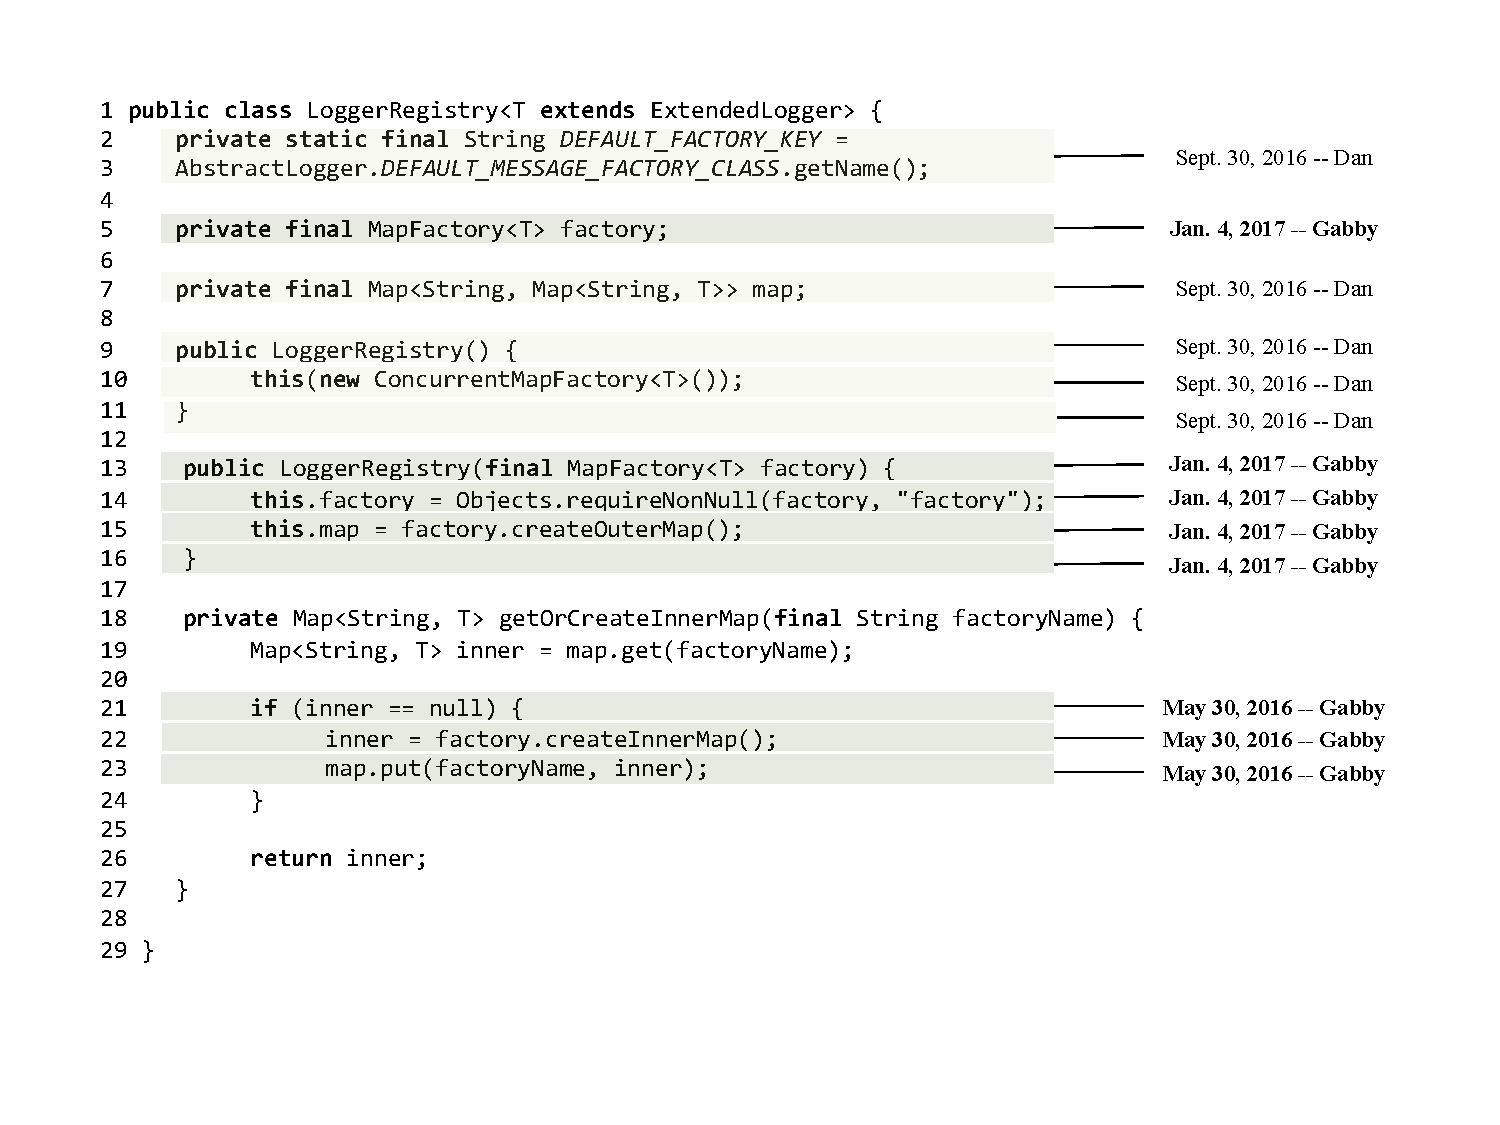
\includegraphics[width=4.5in]{Chapter-6/figs/code.pdf}
	\caption{Mapping of developer source code contributions on one class in an open source repository.}
	\label{fig:code}
\end{figure}

\subsubsection{Concept-Specific Source Code}

To answer RQ\textsubscript{2}, I collected concept-specific code and manually collected lines of code (LOC) added to each repository for each developer from GitHub. 
I define concept-specific source code as code that, according to on-line resources, is relevant to understanding and using the concept in source code. 
Since much of a developer's experience is writing source code, and experience informs knowledge~\cite{bromme1995fusing,argote2011organizational}, I used total LOC as the naive model.

I used the same key concepts identified for the concept inventories to determine what concept-specific code to analyze for. 
For each concept, I used the same resources used to create the concept inventories to determine relevant code to collect from developers' repositories.
In the end, I collected 11 examples of generics usage, 10 examples of exception handling usage, and 12 examples of variables usage.\footnote{The repository that holds the analyzer used can be found at: www.github.com/brittjay0104/APATIANproto} All of the code I collected, along with a description and example for each, is shown in Tables~\ref{tab:var_code}--~\ref{tab:gen_code}. 
I manually checked the added lines reported by GitHub on each developer's repositories to determine LOC for the naive model.

Because Gabrielle took the variables and generics concept inventories, I analyzed her repositories for code that she contributed that related specifically to variables and generics. For example, looking at the code in Figure~\ref{fig:code}, in the class \texttt{LoggerRegistry<T extends ExtendedLogger>}, Gabrielle contributed both variables (lines 5 and 13) and generics code (lines lines 5, 13, and 23). 

The output of the analyzer for each repository is an occurrence count for all contributed concept-specific code and when the most recent contribution for each occurred.
For example, looking at Gabrielle's contributions in \texttt{LoggerRegistry<T extends ExtendedLogger>}, Gabrielle added two variables (a private final field at line 5 and a final parameter at line 13). For each variable she contributed, the analyzer would also note that her most recent contribution for each was in the past couple months.
Prior to dividing the data by features or applying heuristics, I used the list of concept-specific source code outlined in Table~\ref{tab:var_code} (Variables), Table~\ref{tab:excep_code} (Exception Handling), and Table~\ref{tab:gen_code} (Generics) to determine levels of source code usage.

\subsubsection{Source Code Usage Hierarchy}
I analyzed data from 19, 35, and 23 GitHub developers for variables, exception handling, and generics (respectively).
I used all the output from analyzing developers' code repositories to determine which types of concept usage might be more advanced than others. 
Based on frequency of source code usage across repositories and developers for each concept (Figure~\ref{fig:code}), I created a hierarchy of source code usage that outlines what source code collected might be considered basic, intermediate, or advanced. 
Under the assumption that the more something is used the less difficult (and more foundational) it is, I determined which features fit into which category by observing what source code developers used most often versus source code developers use least often. 
For example, only 27\% on the source code we collected included Bounded Type Parameters (Figure~\ref{fig:code}) as opposed to the 99\% of source code included Generic Type Declarations. Therefore, I consider Type Declarations basic usage and Bounded Type Parameters advanced usage. 
I determined thresholds by a leap in the total count of source code usage of more than 100.	
An example concept source code usage hierarchy, along with a more detailed description of the creation process and usage, can be found on-line with the other materials.
% TODO this becomes an Appendix


\subsubsection{Data Features and Heuristics}\label{subsec:prep}

To provide a wider range of generalizable attributes for answer our research questions, I characterized the dependent attributes (Figure~\ref{fig:approach}c) for the models by grouping concept-specific code collected above based on features of the data. 

For example, a feature of type parameter fields and methods (Figure~\ref{fig:code}, lines 5 and 13) that groups them together is Gabrielle wrote new generic code (Declarations) for use by other developers, rather than using existing generic code (Usages) as she did on line 23.
The set of features identified and used among the data are as follows:
\begin{itemize}
	\item \textbf{Levels of Concept Usage:} I computed the Levels of Concept Usage by adding together counts from the types of each concept that would be considered on a basic, intermediate, or advanced level of usage. I used the concept source code usage hierarchy discussed previously. 
	In Tables~\ref{tab:var_code}--~\ref{tab:gen_code}, Basic usage has one star (\textbf{$\star$}) at the end of its description, Intermediate two stars (\textbf{$\star\star$}), and Advanced three stars (\textbf{$\star\star\star$}).
	\item \textbf{Declarations:} I computed Declarations for each concept by adding together counts from the types of concept usage where the developer wrote new concept code for use by themselves or others (i.e. type declarations or new exception type). In Tables~\ref{tab:var_code}--~\ref{tab:gen_code}, Declarations are labeled with a \textbf{(D)} at the end of the description.
	\item \textbf{Usages}: We computed Usage by adding together counts from the types of concept usage where the developer is using code someone else wrote (i.e. method invocations), as opposed to contributing to a new type. In Tables~\ref{tab:var_code}--~\ref{tab:gen_code}, Usages are labeled with a \textbf{(U)} at the end of the description.
\end{itemize}

Because I currently only collect variable declarations, all variable concept-specific code collected for this study falls under Declarations.

Along with the above features, I also defined two heuristics to apply to the feature groups:

\begin{itemize}
	\item \textbf{Recency:} The recency heuristic takes each of the initial attribute values and multiplies each value by 1.0 if the most recent contribution was made in the last week, 0.8 if between one week and one month, 0.6 for 1--6 months, 0.4 for one year, and 0.2 for more than one year.
	For example, if, the total number of declarations made by the developer (Declaration heuristic) is 198 and the most recent declaration was written between one week and one month, the Type Declaration Recency (DeclRecency) heuristic value would be 158.4 (\(198 \times 0.8)\). 
	\item \textbf{Natural Log:} This heuristic calculates natural log of each feature group before and after the recency heuristic is applied.
\end{itemize}

I defined a recency heuristic because previous analyses suggested time may be a factor to consider when modeling knowledge~\cite{johnson2015bespoke}. 
For Gabrielle, if I only analyzed the class in Figure~\ref{fig:code}, Gabrielle contributed a field, private variable, final variable, and parameter; all would be assigned the same recency value (0.6) based on when she made the contribution(s).
Gabrielle contributed 3 pieces of generic code: a type parameter field (line 5), a type parameter method (line 13), and an implicit method invocation (line 23). However, as shown in Figure~\ref{fig:code}, Gabrielle contributed type parameter fields and methods more recently than she contributed implicit method invocations. Therefore, while Gabrielle's type parameter field and method recency value is 0.6, her implicit method invocation recency value would be 0.4.

I applied natural log to the data following the reasoning of Fritz and colleagues, who used natural log in their models to account for the potential for large differences in attribute values~\cite{fritz2010degree}. For example, some repositories returned counts in the thousands for class instantiations but counts of zero for explicit method invocations; this might cause the model to put more weight on the contribution of feature groups and heuristics that include class instantiations than it truly contributes.

\subsubsection{Developer Knowledge Classifications}
Once the attributes have been calculated, I performed discretization to convert the continuous concept inventory score values into intervals of values, or \emph{classes} (Figure~\ref{fig:approach}d)~\cite{fayyad1993multi}. This step became particularly important once I decided to use decision tree learners to answer the research questions -- I discuss the decision to use decision trees later in this section.

Discretization involves iteratively comparing attribute values for each instance and finding the ``best cut'' in the data; each cut is considered a class of the data. A distinguishing feature of this data set is its small size (just a few dozen rows). Hence, I cut the concept inventory scores for each model into two and three classes to answer the research questions. Two classes comes from cutting on the median. I chose three to account for the potential transition between classes~\cite{dreyfus2004five}. For the three way split, with the small data set, I tried to maintain relatively even size chunks while making sure there is some consistency across models (i.e. someone with a score of 7 or above is never a beginner).

The generics data yielded ternary discretization (three classes) and the variables and exceptions data yielded binary discretization (two classes). For data sets with three classes, I labeled each developer as either Beginner, Intermediate, or Expert. For data sets with two classes, we labeled each developer as either Beginner or Expert.	
Based on Gabrielle's concept inventory scores and source code data, she is labeled Expert for both generics and variables. 
We will talk about what the differences in the discretization output might mean in Section~\ref{sec:disc}.

\subsubsection{Attribute Selection}
Once I assigned classifications to each developer, I used developer knowledge classifications to perform Correlation-based Feature Selection (CFS) in Weka, software that provides a collection of machine learning algorithms for data mining.~\cite{Hall:2009:WDM:1656274.1656278}. CFS helps to determine the attributes best suited for each model (Figure~\ref{fig:approach}e)~\cite{hall1999correlation} by pruning irrelevant attributes, leaving only the attributes that correlate the most with the developer's classification.

This analysis runs k-fold cross validation using the attributes passed in; to lower the potential for a model with overestimation bias, I maintained even and sizable chunks by using 4-fold cross validation.	
CFS evaluates each attribute on its predictive ability and uses cross-validation to indicate how stable the best subset of variables is based on how many folds the variable appeared in.
For increased model stability, I used the selection criteria that the attribute appear in two or more folds to be included in decision tree learning.

\subsubsection{Decision Tree Learning}
To answer the research questions, I used decision tree learning. 
More specifically, I used Weka's J48 classifier~\cite{witten1999weka} to create decision trees. 
Wolpert and colleagues~\cite{wolpert1997no} caution that one should not expect any particular algorithm to work best for all possible inputs. Hence, when exploring new data, is it necessary to conduct some experimentation to find useful settings for that data. Accordingly, I ran different analyses and learners to determine which learner was most effective for the data and research goals. Because there are so many machine learning algorithms availble, I neeeded to narrow down the learners I would experiment with. I chose to compare regression, Naive Bayes, and Decision Trees based on prior work with similar goals of making software development-related predictions~\cite{menzies2004assessing,menzies2007data,heckman2009model,fritz2010degree}. I found decision trees to be optimal for answering the research questions along with being more human readable.

Another motivation for using decision trees as opposed to regression or Naive Bayes is the relatively heightened error tolerance provided by decision tree learners. Because I only used public repository contributions, the data collected may have attributes with no data. For example, upon analyzing a developer's repositories I may find no occurrences of generic type declaration due to the fact that the developer has written generic type declarations in a context not being analyzed (i.e. local software projects). Using decision trees allows us to see meaningful relationships in the data, regardless of any data that may be erroneous or inaccurate.
% Based on the results from decision tree learning, I next .

\section{Knowledge Models}\label{sec:eval}

Based on developer classifications and the full set of attributes, CFS identified the following subset of attributes that fit my selection criteria:
\begin{itemize}
    \item \textbf{Variables} -- Public Variables
    \item \textbf{Exceptions} -- Advanced Exceptions, Try Statements Recency, Finally Blocks Recency, and Throws Methods
	\item \textbf{Generics} -- LOC, Generic Type Declarations, and Generic Type Declarations Recency
\end{itemize}

I created a decision tree model for each concept with all the concept-specific attributes above to answer RQ\textsubscript{1}. To answer RQ\textsubscript{2}, I created a LOC only model, when LOC met the attribute selection criteria, to compare to the concept-specific models.
The values for each model's \emph{precision}, \emph{recall}, \emph{F-Score}, \emph{TP (True Positive) Rate}, and \emph{FP (False Positive) Rate} are shown in Tables~\ref{tab:vars},~\ref{tab:exceptions},~\ref{tab:gen}, and~\ref{tab:loc}. The resulting decision trees can be found in Figures~\ref{fig:vars},~\ref{fig:excep}, and~\ref{fig:gen}.

\begin{table}
	\centering
	\caption{Variables Model Accuracy}
	\label{tab:vars}
	\begin{tabular}{llll}
		\toprule
		\multicolumn{4}{c}{\textbf{Public Variables}}                               \\
		\cmidrule(lr){1-4}
		& \textbf{Beginner} & \textbf{Advanced} & \textbf{Total} \\
		\midrule
		\textbf{Precision} & 0.571             & 0.667             & 0.627          \\
		\textbf{Recall}    & 0.500             & 0.727             & 0.632          \\
		\textbf{F-Score}   & 0.533             & 0.696             & 0.627          \\
		\textbf{TP Rate}   & 0.500             & 0.727             & 0.632          \\
		\textbf{FP Rate}   & 0.273             & 0.500             & 0.404   \\
		\bottomrule
		
	\end{tabular}
\end{table}

\begin{table}
	\centering
	\caption{Exceptions Model Accuracy}
	\label{tab:exceptions}
	\begin{tabular}{llll}
		\toprule
		\multicolumn{4}{c}{\textbf{\begin{tabular}[c]{@{}c@{}}Advanced, Try Statement Recency, \\ Finally Block Recency, Throws Method \end{tabular}}} \\
		\cmidrule(lr){1-4}
		& \textbf{Beginner}                 & \textbf{Advanced}                 & \textbf{Total}                 \\
		\midrule
		\textbf{Precision}                 & 0.789                             & 0.750                             & 0.771                          \\
		\textbf{Recall}                    & 0.789                             & 0.750                             & 0.771                          \\
		\textbf{F-Score}                   & 0.789                             & 0.750                             & 0.771                          \\
		\textbf{TP Rate}                   & 0.789                             & 0.750                             & 0.771                          \\
		\textbf{FP Rate}                   & 0.250                             & 0.211                             & 0.232                         \\
		\bottomrule
	\end{tabular}
\end{table}

\begin{table}
	\centering
	\caption{Generics Model Accuracy (Non-LOC)}
	\label{tab:gen}
	\begin{tabular}{lllll}
		\toprule
		\multicolumn{5}{c}{\textbf{Declarations and DeclRecency (Generics)}}                                                            \\
		\cmidrule(lr){1-5}
		& \textbf{Beginner} & \textbf{Intermediate} & \textbf{Advanced} & \textbf{Total} \\
		\midrule
		\textbf{Precision} & 0.667             & 0.727                 & 0.875             & 0.729          \\
		\textbf{Recall}    & 0.333             & 0.889                 & 0.875             & 0.739          \\
		\textbf{F-Score}   & 0.444             & 0.8                   & 0.824             & 0.715          \\
		\textbf{TP Rate}   & 0.333             & 0.889                 & 0.875             & 0.739          \\
		\textbf{FP Rate}   & 0.059             & 0.214                 & 0.133             & 0.146         \\
		\bottomrule
	\end{tabular}
\end{table}

\begin{table}
	\centering
	\caption{Generics Model Accuracy (LOC only)}
	\label{tab:loc}
	\begin{tabular}{lllll}
		\toprule
		\multicolumn{5}{c}{\textbf{LOC (Generics)}}                                                         \\
		\cmidrule(lr){1-5}
		& \textbf{Beginner} & \textbf{Intermediate} & \textbf{Advanced} & \textbf{Total} \\
		\midrule
		\textbf{Precision} & 0.5               & 0.636                 & 0.875             & 0.684          \\
		\textbf{Recall}    & 0.333             & 0.778                 & 0.875             & 0.696          \\
		\textbf{F-Score}   & 0.4               & 0.7                   & 0.875             & 0.683          \\
		\textbf{TP Rate}   & 0.333             & 0.778                 & 0.875             & 0.696          \\
		\textbf{FP Rate}   & 0.118             & 0.286                 & 0.067             & 0.166         \\
		\bottomrule
	\end{tabular}
\end{table}

\begin{figure} [h]
	\centering
	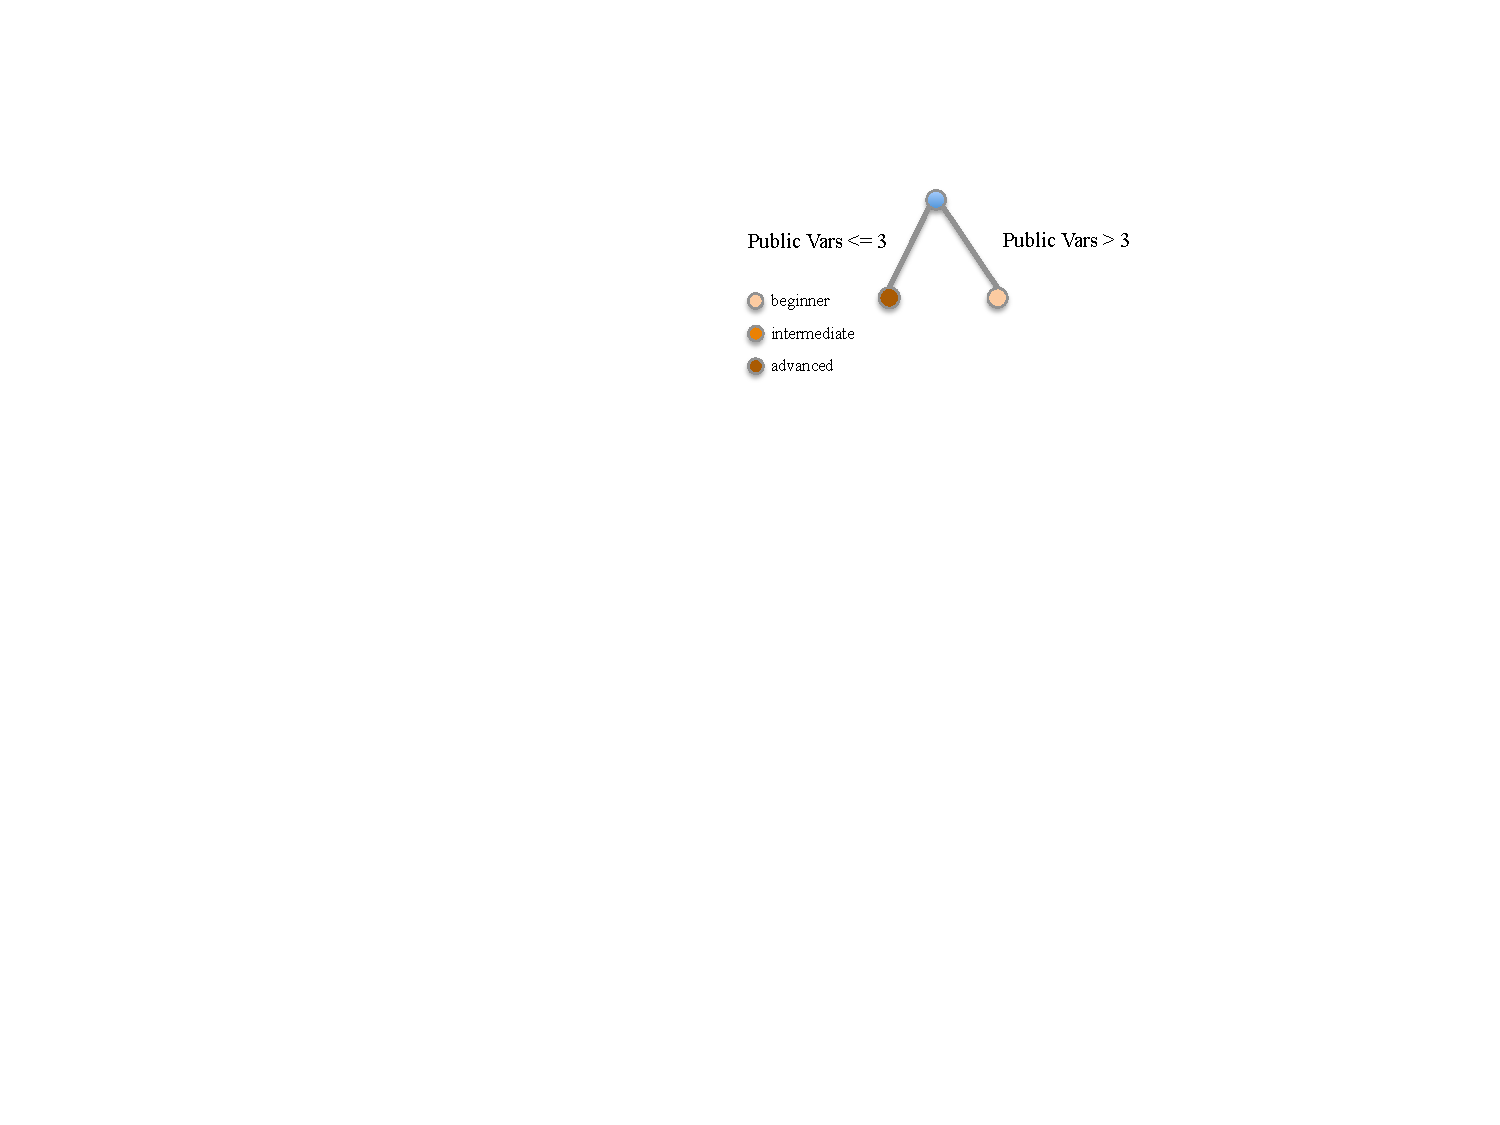
\includegraphics[width=3.5in]{Chapter-6/figs/variables.pdf}
	\caption{Variables decision tree model.}
	\label{fig:vars}
\end{figure}

\begin{figure} [h]
	\centering
	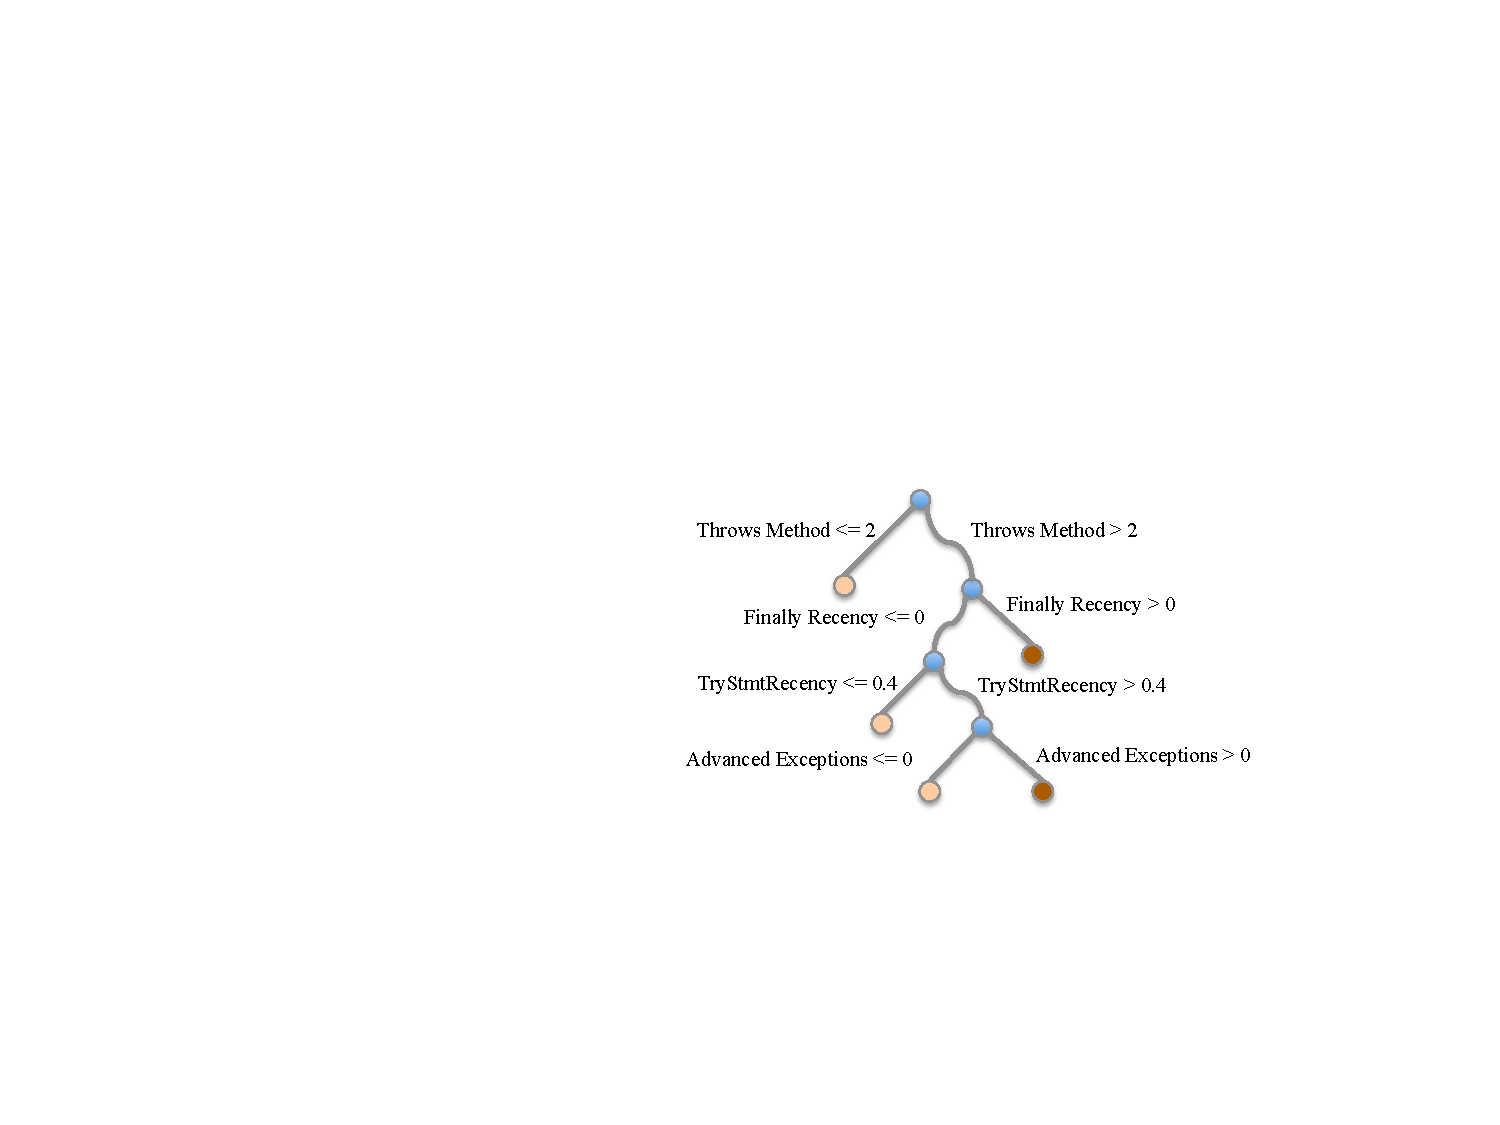
\includegraphics[width=3.5in]{Chapter-6/figs/exceptions.pdf}
	\caption{Exceptions decision tree model.}
	\label{fig:excep}
\end{figure}

\begin{figure} [h]
	\centering
	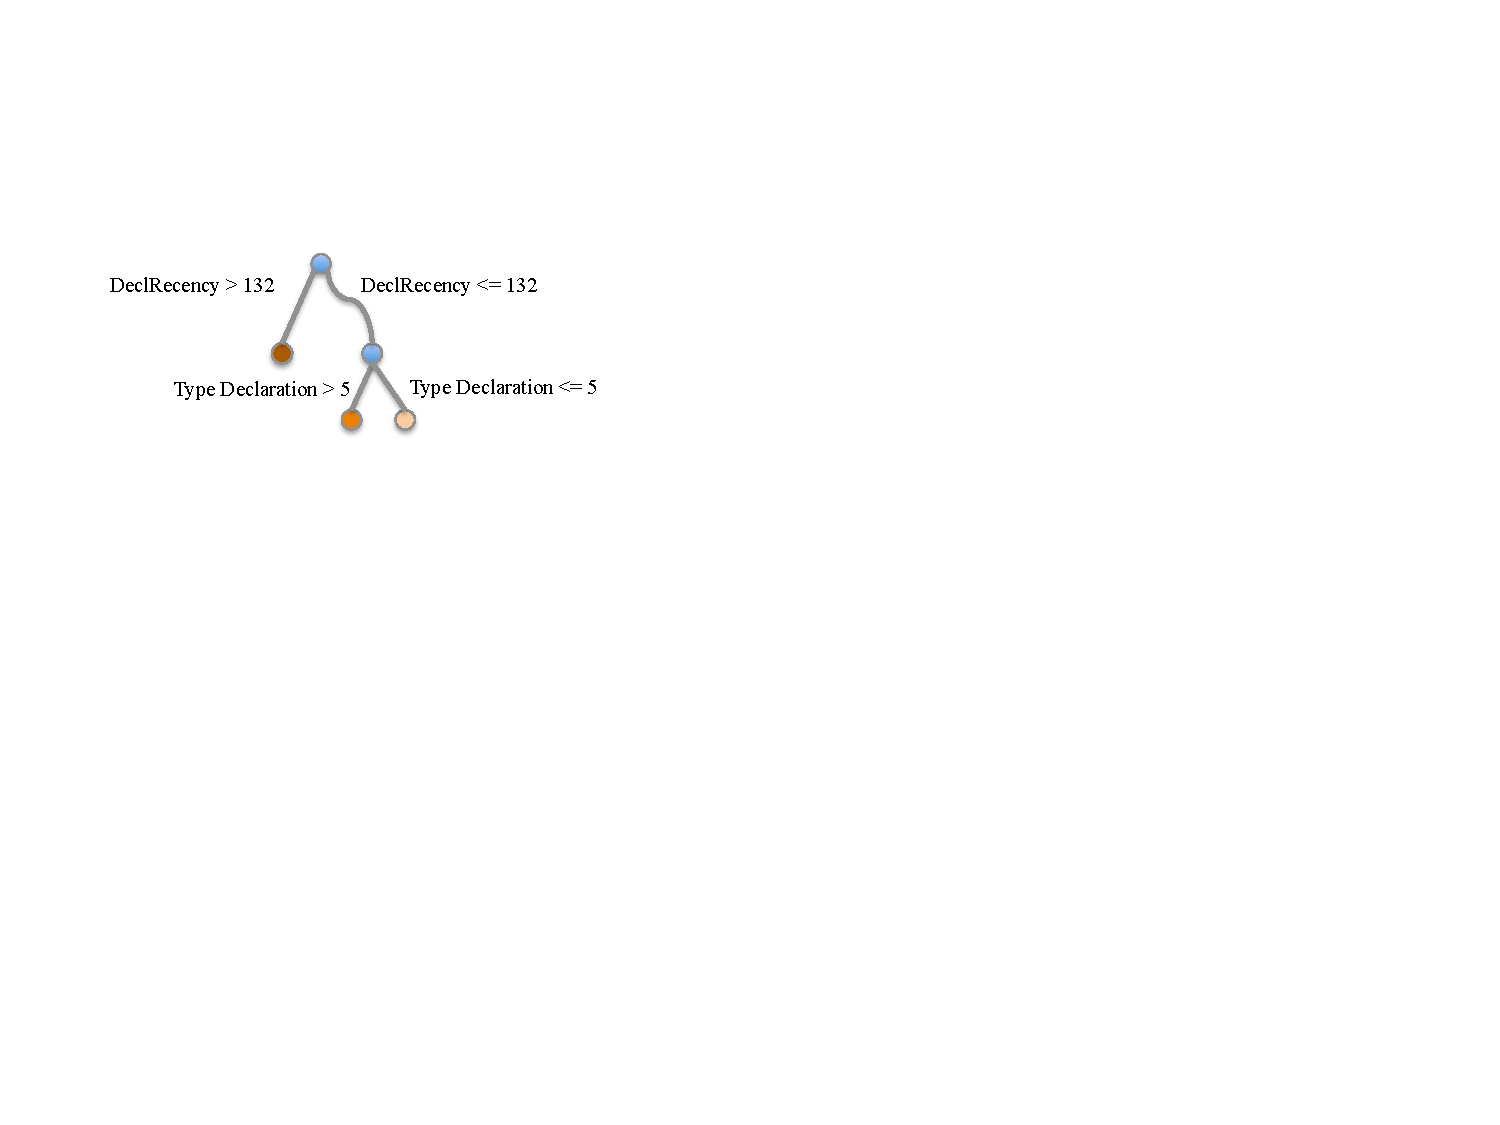
\includegraphics[width=3.5in]{Chapter-6/figs/generics.pdf}
	\caption{Generics decision tree model.}
	\label{fig:gen}
\end{figure}


\subsection{RQ\textsubscript{1} Findings}

All four decision tree models had total precision, recall, and F-Score of at least 60\%, suggesting these models correctly classified developers at least 60\% of the time. Even the model built using LOC only (Figure~\ref{fig:loc}) provided accurate predictions. 
This supports existing research that suggests all of our experiences contribute to our overall knowledge~\cite{argote2011organizational}; my findings quantify this notion, showing it is possible to use developer experience to predict their knowledge.
The models also exhibit low FP rates, with a median FP rate of 19.9\%. I observed the highest FP rate with the variables model (Figure~\ref{fig:vars}); I will discuss limitations that may have caused the difference in FP rate for the variables model in Section~\ref{sec:challenges}.

Based on the attributes used in the decision trees shown in Figure~\ref{fig:gen} and Figure~\ref{fig:excep}, how recently concept-specific code was contributed can also affect conceptual knowledge. Based on the recency heuristic, for example, a higher DeclRecency (Figure~\ref{fig:gen}) value suggest more recent code contributions related to declaring generic types. This suggests that determining a developer's knowledge of generics would involve observing both declarations and recent experience with declarations. For exceptions, recency matters for some attributes, such as \texttt{try} statements and \texttt{finally} blocks, while it is not as important for others, such as usage of advanced exceptions language features. For variables, recency also did not appear to improve classification -- the variables model only includes the declaration of variables, which may have affected the ability to build an accurate and convincing model. 
% I will discuss some explanations for these results and ways to potentially improve the variables model in Section~\ref{sec:challenges}.

\vspace{1em}

\fbox{%
	\parbox{0.9\linewidth}{%
		\noindent\textbf{\textit{These findings suggest that source code can be used to classify how much developers know about programming concepts better than random chance.}}
	}%
}
\vspace{0.5em}


\subsection{RQ\textsubscript{2} Findings}

All three of the models that we trained using concept-specific attributes classified developers better than random chance ($>$ 50\%).
As for comparing the concept-specific models to a more naive model, after using CFS during data analysis, I was able to identify relevant attributes before running cross-validation during tree building. For two of the three concepts evaluated, LOC did not appear in enough folds during attribute selection to be considered during decision tree learning. Even with the variables data, which only included various attributes pertaining to variable declaration, the most meaningful attributes were concept-specific. The only data set in which LOC appeared in more than two folds was the generics data set. This suggests that in some cases, LOC is not predictive of developer concept-specific knowledge.

Upon closer examination of the generics models, overall model performance is higher in the Type Declaration model (74\%) than the LOC model (70\%), with increased precision and F-Score for beginner (\(+ 0.167\), \(+ 0.04\)) and intermediate (\(+ 0.09\), \(+ 0.1\)) classification and increased total precision (\(+ 0.05\)), recall (\(+ 0.04\)), and F-Score (\(+ 0.03\)). 
The only scenario where the LOC model outperformed the Declarations model was when classifying developers with advanced generics knowledge (Table~\ref{tab:gen}). 
These findings suggest that although both LOC and concept-specific code can both be used to predict conceptual knowledge, concept-specific code increases overall model accuracy and precision.

\vspace{1em}

\fbox{%
	\parbox{0.9\linewidth}{%
		\noindent\textit{\textbf{These findings suggest that concept-specific code improves model performance when compared to a naive model.}}
	}%
}
\vspace{0.5em}


\section{Implications}\label{sec:disc}
The ability to predict developer conceptual knowledge using attributes collected from source code opens the doors for exploring the possible applications, including the ability to adapt tool notifications to developer knowledge. 
I discuss the potential for adapting tool output and some of the other possible applications for these findings in detail below.
% Predictions for tools adaptations (building on prior work)

\subsection{Program Analysis Tool Output}
This study was motivated by the study reported in Chapter~\ref{chap:theory}, which posed a theory regarding the challenges developers encounter when attempting to understand, and eventually resolve, tool notifications~\cite{johnson2016cross}. The theory stated that the challenges developer encounter stem from gaps and mismatches between their knowledge and how tools communicate. One way to assess this theory is to explore the ability, and effectiveness, of adapting tool notifications to the knowledge of the developer using them.

% When tools communicate with developers, at the lowest, most fundamental level, they are communicating about \emph{programming-oriented concepts}, which relate to how the source code maps to programming language concepts~\cite{van2004concepts,biggerstaff1994program}. For simplicity, I refer to these concepts simply as programming concepts.
% Existing research on experience as a representation for knowledge~\cite{argote2011organizational,bromme1995fusing} and using source code contributions to predict developer knowledge of a code base~\cite{fritz2010degree} led to research questions related to using source code to predict concept-specific knowledge.

The ability to accurately classify developers' conceptual knowledge is the first step towards being able to provide meaningful notification adaptations. If a tool can automatically ascertain how much a developer knows about the concepts relevant to a given notification, it can better tailor the information provided to the information needed by that developer. The next step is to determine what a meaningful adaptation for a given developer classification looks like; this work is described in detail in Chapter~\ref{chap:improve}.

Another way that developer conceptual knowledge can be utilized by program analysis tools is to improve developers' experience when first using notifications used by the tool~\cite{johnson2015bespoke}. One of problems that have been identified with program analysis tools, especially static analysis tools, is the high volume of notifications that are sometimes presented~\cite{Johnson:2013:Why}. We can use developer conceptual knowledge to determine the notifications to prioritize. A common way current tools prioritize notifications is by problem severity, however, such strategy may not be enough to ensure a positive first experience. Also, findings from Chapter~\ref{chap:theory} suggest developers do not always agree with the prioritization used by tools~\cite{johnson2016cross}. Tools could improve the first experience by first presenting developers with notifications the tool knows they can solve based on the concepts they understand best.

\subsection{Industry \& Education Practices}
% TODO - introduce this section

For any given defect, there are one or more programming concepts relevant to understanding and being able to resolve that defect. Similar to work on code review assignment~\cite{balachandran2013reducing}, another potential application for my proposed approach for predicting conceptual knowledge is to assign the best developer to resolve a defect or complete a code review. Although knowledge of the code base is important~\cite{fritz2010degree}, my research suggests knowledge of concepts relevant to the defect or code of interest is also important~\cite{johnson2016cross}. My approach can be combined with other approaches, such as those that look at the developer's familiarity with the code base~\cite{fritz2010degree}, to assign defects to developers that are most likely to be able to resolve them. 	

The ability to predict developer knowledge also opens the door for the potential to more effectively assign  teams in industrial and educational settings. For example, if the design and implementation of a project or piece of functionality requires specific conceptual knowledge, analysis of developers' existing source code can yield information for ensuring someone with the necessary knowledge is on that team.
Along the same lines, my approach can be useful for determining effective pair programming pairs. 
Pair programming is an effective way of transferring knowledge~\cite{plonka2015knowledge} and fostering tool discovery~\cite{murphy2011peer}, both of which can aide in defect resolution. Knowledge transfer is more likely to occur when the developers paired together differ in experience (i.e. one is novice and one is expert). Furthermore, a previous study on pair programming found that the productivity provided by pair programming can drop substantially when it comes to problem solving if both programmers have experience with the problem at hand; this is especially true if the experiences are recent and has not had a chance to be forgotten~\cite{lui2006pair}. When it comes to pairing developers for a specific task, our approach can be useful for determining which developer is more expert in the concepts relevant to the task at hand. 
%~\todo{May be talk about interview screening and prep?}

\section{Lessons Learned}\label{sec:challenges}
Even with a glimpse into the possibility of modelling conceptual knowledge, there are limitations to my current approach and challenges to overcome.

% TODO think about how this is organized
\subsection{Limitations}
One limitation to my approach is that it relies solely on source code available in public repositories; not all developers have public repositories and usually not all the code a developer has written is stored in one.
Along the same lines, while analyzing developer source code can provide insights into conceptual knowledge, this may not be entirely representative of everything the developer knows about a given concept, or more importantly the notifications they encounter, which could lead to initially inaccurate models.

Another limitation to the findings presented in this chapter is that I built the models with a relatively small numbers of developers. Typically machine learning is done with large data sets, however, due to the nature of the data collected I ended up with smaller data sets (~20--30 data points). I mitigated this limitation by using decision tree learning, which has been found to work well with atypical data sets~\cite{zhang2005missing,kotsiantis2007supervised}.

One goal as I developed this approach was to provide a range of attributes relating to each concept to increase the likelihood that we are being exhaustive of relevant and possibly predictive code features. A limitation to my approach in this regard is how I dealt with a fundamental concept like variables, which can include a large range of relevant features. In this work, I decided to focus on various aspects of declaring a variable, such as data types and variable visibility, to narrow down the space of attributes being analyzed. I believe this led to the less-than-compelling model for variables conceptual knowledge found in Section~\ref{sec:eval}. Although the model is not as compelling or complex as the others, the variables model still suggests that using source code to predict concept knowledge is better than random chance or a naive model.
% not all repos 100\% Java
Another limitation is that for a small subset of developers, at least one repository was not 100\% Java. Repositories that fit into this category ranged from 42\% - 97\% Java.
Currently, my approach has only been evaluated on developers' knowledge of Java concepts, therefore a LOC model including non-Java code might have affected the results. 

\subsection{Challenges}
Mirroring the small data set limitation, one challenge to using my approach is getting enough data from the developer, especially if the developer does not have code in public repositories. One way to deal with this challenges is to modify the approach to work in on local copies and in real-time to detect developer concept-specific contributions in projects not stored in repositories.

Another challenge that comes with using my approach is determining how to deal with both fundamental and nuanced programming concepts. The findings in this chapter suggest that it may be more difficult to build an exhaustive and accurate model for fundamental concepts than it is for nuanced concepts. This may suggest that there are ways that concepts group together that can may affect how one should approach determining relevant code to collect. For example, the code we collected for variables matches the information provided on the primary sources of variables-related concepts used for the concept inventory. However, because declaring variables is necessary in most programs, there may be a need to incorporate other information such as notifications pertaining to variables the developer encountered, to get the best idea of what developers really know about variables.

Along the same lines, another challenge for my current approach is the ability to generalize across concepts. For the most exhaustive models, we can see similarities such as the fact that recency is generally important. However, it is not obvious beyond that if there is a way to general what is important to focus on when classifying developers based on their code contributions. A good starting point for work in this area would be to determine the possibility of generalizing across a subset of concepts with similar characteristics, such as splitting concepts by simple, fundamental concepts, such as variables, methods, and classes, and more complex, nuanced concepts, such as generics, exception handling, and concurrency.

% TODO more for transition here??
Despite the limitations and challenges associated with my proposed approach, the results of this study provided insights that can be used to further my research on improving the notifications tools use. In the next Chapter, I discuss how we can use developer knowledge to improve communication between developers and their tools.
\chapter{Knowledge-Based Communication}
\label{chap:improve}

Based on findings from previous studies, tools do not always effectively communicating with developers.
One reason this occurs is because of differences between developer knowledge and the information provided by notifications~\cite{johnson2016cross}.
Perhaps if tools could ascertain how much developers know about the concepts present in the information they provide, tools could provide feedback to better support developers in understanding and resolving defects.
The previous chapter suggested the ability to use developer source code contributions to predict how much they know about the concepts in tool notifications.

\textit{Given the ability to classify developers based on their knowledge of programming concepts, I propose improving the communication between tools and developers by providing knowledge-based notifications.}
Knowledge-based notifications would present information to developers based on how much they know about the concepts relevant to the defect.
To my knowledge, there are no existing studies that have explored adapting the information provided by tool notifications.

Despite notification adaptation being a new research area, adaptive user environments are becoming pervasive in research and practice~\cite{zou2008adapting, amershi2007unsupervised, stamper2009unsupervised}. 
Adaptive User Interfaces (AUI) use the experiences of users to adapt to better support the user.
Most relevant to this research are the models proposed by Zou and colleagues for adaptive menus in Eclipse~\cite{zou2008adapting}.
Similarly, this research explores using source code and machine learning to predict user knowledge but for adaptive tool notifications.


In this chapter, I discuss research that explores possible notification adaptations and the ability to improve communication by improving the support provided by tools to fill knowledge gaps and match developer expectations. 
To evaluate this proposal, I borrowed from existing research on expertise and problem solving to determine potential notification adaptations to evaluate and how they map to expertise.
I used the same concepts used in previous chapters to create and evaluate knowledge models: variables, exception handling, and generics.
I found notifications that communicate primarily about various aspect of these concepts, focusing on notifications that communicate about defects that are found in real software projects~\cite{ayewah2007evaluating, zheng2006value}.

I conducted 14 user studies with students and professional developers with various backgrounds and knowledge regarding the concepts of interest to evaluate their ability to resolve notifications designed for their level of expertise. This study was designed to evaluate the following hypotheses and research question:
\begin{itemize}
    \item [H\textsubscript{1}] Knowledge-based notifications can decrease the time required for notification resolution.
    \item [H\textsubscript{2}] Knowledge-based notifications increase developer likelihood of resolving notifications. 
    \item [H\textsubscript{3}] Knowledge-based notifications decrease developer attempts to resolve notifications.
    \item[RQ] Do developer adaptation preferences match expectations, based on existing literature?
\end{itemize}


\section{Proposed Approach}

For adaptive tool notifications to be realized, it is necessary to determine how tools should present information to developers. Previous research suggests one thing to consider when presenting information regarding a defect is the knowledge of the developer~\cite{johnson2016cross}.
To evaluate H\textsubscript{1} -- H\textsubscript{3}, I conducted user studies where I presented developers with adapted notifications and asked them to resolve each. In this section, I will outline the related research I used to create the adapted notifications and the approach I used to evaluate notification adaptations.

\subsection{Notification Adaptations}

Existing research on notification design focuses on the general information needs of all developers, regardless of their knowledge regarding the notification or its concepts~\cite{smith2015questions, barik14, robillard2014recommendation}. Therefore, there is no existing work that has examined notification design for expertise. 

% TODO add this stuff to related work chapter ??
There does exists work in other fields that has examined problem solving and debugging in relation to programmer expertise~\cite{larkin1980expert, mckeithen1981knowledge, Wiedenbeck:1993:Mental}. I used this existing research to inform the design of the adapted notifications for each level of expertise, and help answer my research question. Based on existing research, I designed knowledge-based notifications using the following criteria:
\begin{itemize}
    \item Notifications designed for developers classified as intermediate and expert for a given concept provide brief notifications with goal statements to communicate the problem.
    \item Notifications designed for developers classified as novice for a given concept provide more detailed notifications with goal statements and subgoals to communicate the problem.
    \item All notifications include examples and links relevant to the problem and its solution.
\end{itemize}

% Determining number of adaptations to design
The previous chapter on classifying developers suggested that for some concepts, progress to expertise is a three stage progression. Previous research found that there is typically homogeneity within expertise groups (novice, intermediate, expert) but that strategy selection and usage is based on expertise~\cite{mckeithen1981knowledge}. This research also found that the intermediate and expert groups exhibited similar strategies.  

For the user study, I chose to design notifications for a novice and expert split rather than novice, intermediate, and expert. I made this decision because 1) designing 3 notifications per defect would have led to longer sessions, 2) the models created in Chapter~\ref{chap:experience} suggest only 2--3 knowledge groupings per concept, and 3) existing research suggests that intermediate and expert programmers solve problems in similar ways~\cite{mckeithen1981knowledge}.

The adaptation provided for each classification should be meaningful to that expertise group. There exists research that has explored the differences between novice and expert problem solving in STEM domains~\cite{larkin1980expert, Wiedenbeck:1993:Mental}. Using this research, I determined possible adaptations for novice and expert developers.

Larkin and colleagues found that experts in STEM domains have common foundations when problem solving~\cite{larkin1980expert}. They found that experts use experience to work from a goal to a solution, while novices required a goal and subgoals to reach a solution. Similarly, Wiedenbeck and colleagues have done extensive work on expertise-based problem solving~\cite{wiedenbeck1985novice,Wiedenbeck:1993:Mental}. They posed five characteristics in expert mental representations, most of which novices lack:

\begin{itemize}
    \item \textbf{It is hierarchal and multi-layered.} This means experts have an understanding of high level program structure and goals as well as low level data structures.
    \item \textbf{It has explicit mappings between layers.} Experts also have mappings between program goals and data structures used to achieve them.
    \item \textbf{It has a foundation.} At the foundation of expert mental representations is the ability to recognize basic patterns or plans.
    \item \textbf{It is internally well-connected.} Experts understand how components in the code work together.
    \item \textbf{It is well grounded in program text.} Experts are able to easily relate the various parts of their mental representations, such as an abstract plan, to the source code.   
\end{itemize}


% Separating problem and goal, adding subgoals
Most notifications provided by state-of-the-art tools provide a problem statement when communicating about a defect. However, my previous research suggests current notifications do not always communicate effectively.
Research in other STEM fields suggests that when problem solving, experts work from a goal to solution~\cite{larkin1980expert}. Therefore, the notifications modified for experts will provide a goal statement rather than a problem statement. The same research found that novices require a goal and set of subgoals that help them achieve the goal to reach a solution. Therefore, notifications modified for novices included a set of general subgoals for resolving the defects. Novice notification also include the problem statement used by FindBugs and the compiler.

% How did I determine goal statement?
I determined the goal statement for each notification by determining the general solution being suggested by the problem statement. For example, the goal statement in Figure~\ref{fig:expert} is based on the problem statement provided for raw type compiler warnings. However, the goal speaks to resolution, letting the developer know she needs to ``Correct the creation and/or initialization for the generic collections.'' There is also a link present, which is active and links to a top search page on the web providing information regarding generic collections, if needed.
% TODO may be more realted studies for here
I provided links throughout the expert and novice notifications based on previous studies that suggest developers often leave their working context to search the web for information~\cite{johnson2016cross,nasehi2012makes}.

% How did I determine subgoals
I determined the subgoals for each notification by determining a) the possible solutions to the defect, b) how to achieve those solutions, and c) how to generalize all of the above.
It is important to maintain a realistic environment with realistic information, therefore the ability to generalize the information to other code snippets with the same defect was the most important. For example, for the notification shown in Figure~\ref{fig:novice}, the subgoals provide generally applicable fix options and provide steps, links, and examples. Also, most importantly, these fixes would generally apply to this defect no matter what code was implemented.

% Adding examples/possible fixes
Developers use examples to understand and resolve problems in code; often they go to sources like StackOverflow~\footnote{\url{https://stackoverflow.com/}} to find examples with explanations as most tool notifications do not include examples~\cite{nasehi2012makes}.
My previous research also found that professional developers like having insights regarding possible fixes to the problem~\cite{johnson2013don,johnson2016cross}.
Therefore, I included examples in all of the notifications. I primarily used StackOverflow to find code examples for the notifications. I also used the same resources used to create the concept inventories in Chapter~\ref{chap:assess}.

Finally, to help mitigate notification familiarity bias, which was found to be relevant to notification understanding and resolution~\cite{johnson2016cross}, I only presented participants with the modified notifications. This included disabling the relevant compiler notifications, which are familiar notifications for participants. 
Example modified notifications are shown in Figure~\ref{fig:novice} and Figure~\ref{fig:expert}.

\begin{figure}
	\centering
	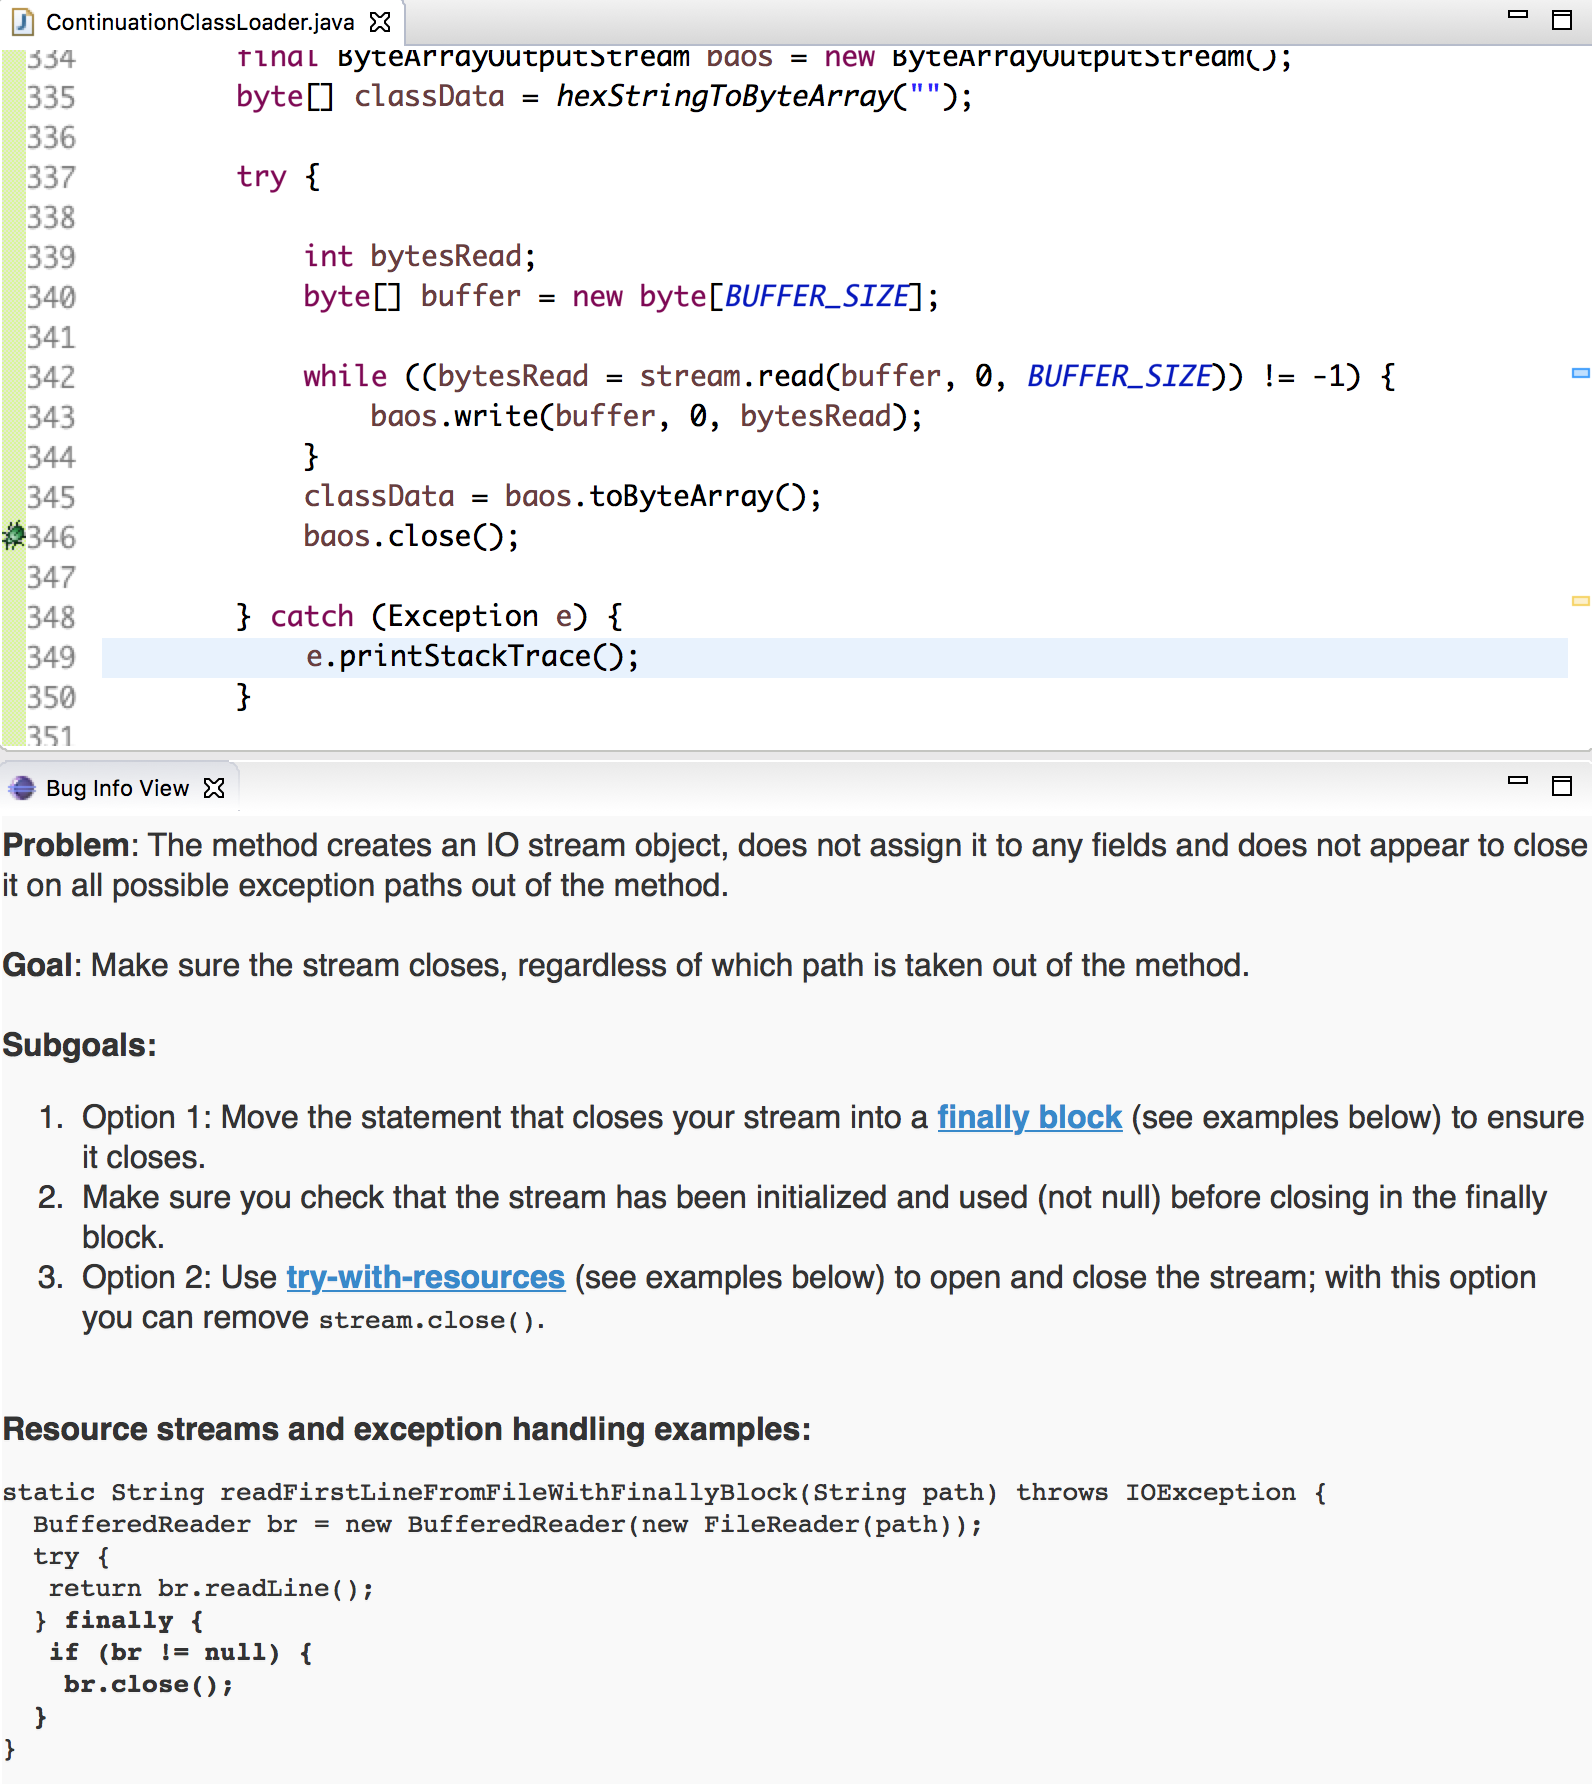
\includegraphics[width=5.5in]{Chapter-7/figs/novice}
	\caption{A notification modified for a developer classified as a novice in  exception handling.}
	\label{fig:novice}
\end{figure}

\begin{figure}
	\centering
	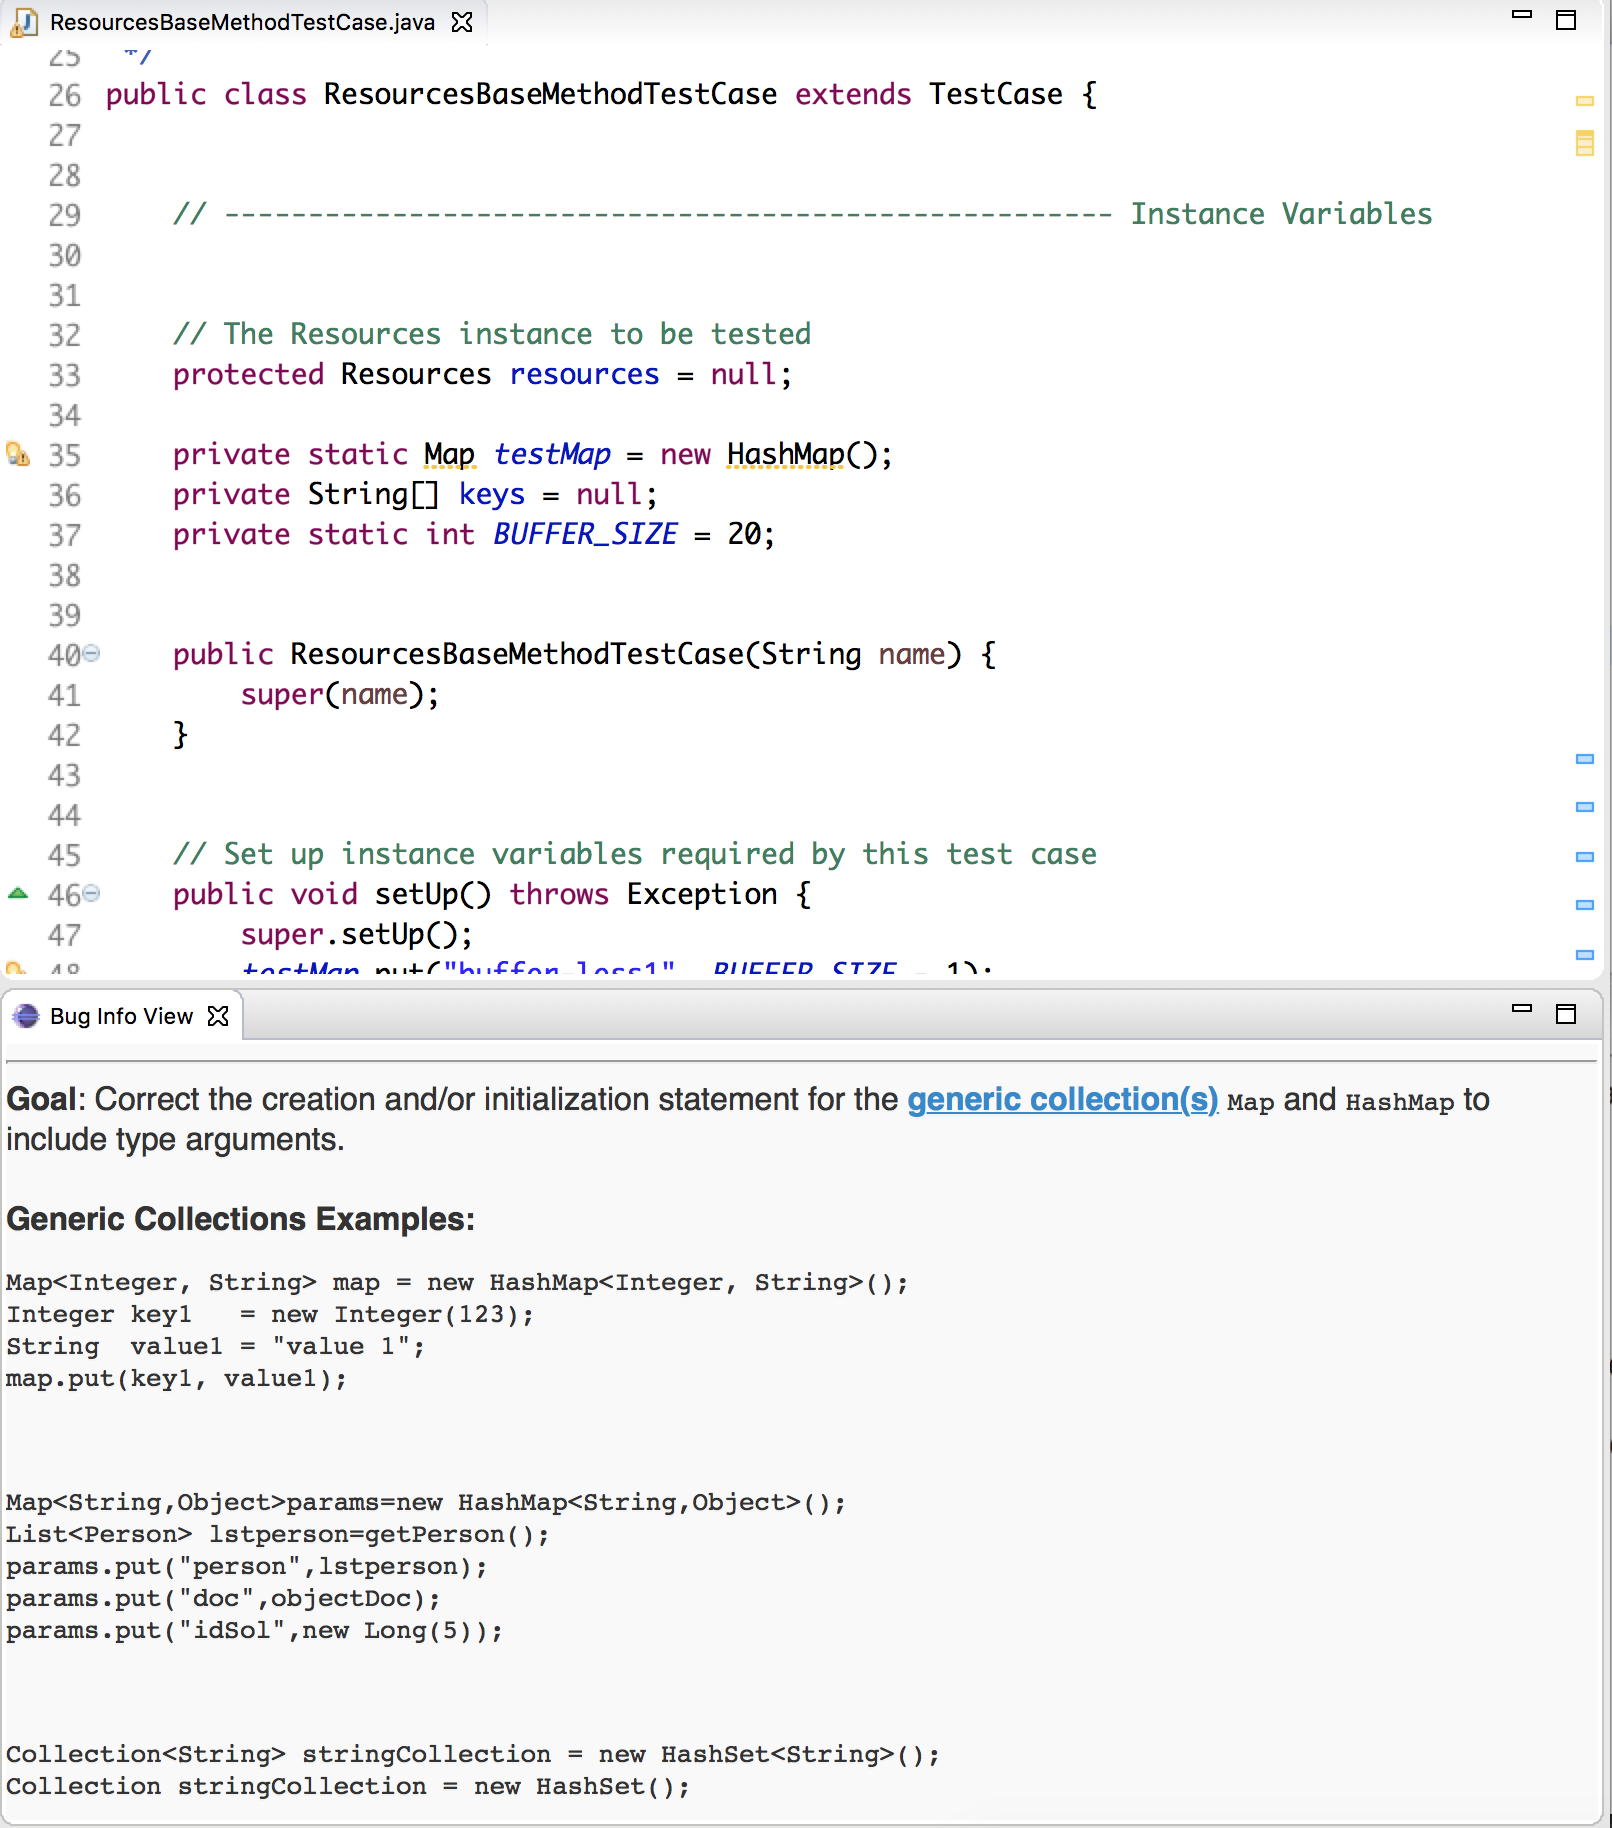
\includegraphics[width=5.5in]{Chapter-7/figs/expert}
	\caption{A notification modified for a developer classified as an expert in  generics.}
	\label{fig:expert}
\end{figure}

% provided insights into what examples I should include -- due technical and time limitations, used examples available online as-is. There exists technologies that can incorporate context-specificity into examples but evaluating availability of examples in notification rather than if they should be context specific.


% Further improved examples using attributes of good responses on StackOverflow~\cite{nasehi2012makes}:
% \item concise code
% \item use question context
% \item highlight important elements
% \item step-by-step -- this is general, based on research that suggests novices benefit more from step by step, part of novice notification design.
% \item links to extra resources
% \item multiple solutions -- why I included multiple examples when possible for each notification
% \item inline documentation
% \item solution \& API implications -- incorporated when necessary (give example?)


\subsection{Notification Selection}

Using the criteria outlined above, I modified 9 program analysis tool notifications from FindBugs and the Eclipse Java compiler, the same tools used in my previous study. I excluded ECLEmma to scope the current problem and solution to textual notifications. For each notification, I created a novice version and an expert version.

% how did I determine what defects to look for initially?
To determine the notifications for the user study, I attempted to find pre-existing defects in open source software. To narrow my search, I focused on defects that have been found to frequently appear in real world software projects~\cite{ayewah2010google}. 
I narrowed my search down to mature projects that were already Eclipse projects, could be relatively easily imported and compiled, and contains code snippets with libraries that are more likely to be familiar to developers.

% how did I find those defects and others to include?
Once I imported the projects, I analyzed the projects for compiler errors and warnings pertaining to the concepts of variables, exception handling, and generics.
I also ran FindBugs on each project to find defects pertaining to the concepts.
I went through the relevant notifications one by one to find code snippets that are not dependent on a large number of other classes and contain libraries and functionality that are familiar to the developer. The latter criteria was to mitigate the threat of developers looking at code that is not their own.

After analyzing a number of projects, I chose to go with the Java Collections library. I was able to find existing notifications from FindBugs and the compiler relevant to the concepts of interest. Because I needed enough notifications to populate my user study, I sometimes had to inject defects into the source code. When this was done, I chose code snippets where only minimal changes led to the introduction of the defect, error, or warning. Also, much of the code used in the library, and the functionality the library is written for, are familiar to developers regardless of their contributing to that code base.
The final set of defects used in the study can be found in Table~\ref{table:notifications}. For each notification in the table, I created a novice and expert version, for a total of 18 notifications.

\newcolumntype{g}{>{\columncolor{gray!40}}l}

\begin{table}[]
\centering
\caption{Notifications used in the user study.}
\label{table:notifications}
\begin{tabular}{lgg}
\toprule
\rowcolor{white}
                            & \textbf{Problem}                                                                                                         & \textbf{Tool} \\
\midrule
\rowcolor{white}
\textit{Variables}          & Unwritten field                                                                                                          & FindBugs      \\
                            & Unused field/parameter                                                                                                   & FindBugs      \\
    \rowcolor{white}
                            &   Incompatible types              & FindBugs               \\
\textit{Exception Handling} & Unhandled exception type                                                                                                 & Compiler      \\
\rowcolor{white}
                            & Method may fail to close stream on exception                                                                            & FindBugs      \\
                            & New exception not thrown                                                                                                      & FindBugs      \\
\rowcolor{white}
\textit{Generics}           & \begin{tabular}[c]{@{}l@{}}Inferred type argument(s) do not conform to the \\ bounds of the type variable(s)\end{tabular} & Compiler      \\
                            & \begin{tabular}[c]{@{}l@{}}Raw types: references to generic types should be \\ parameterized\end{tabular}               & Compiler      \\
\rowcolor{white}
                            & Cannot convert generic types                                                                                            & Compiler    \\
\bottomrule
\end{tabular}
\end{table}

\subsection{Adaptation Evaluation}

Once I had a set of modified notifications, I developed a wizard-of-oz plug-in to evaluate to evaluate H1, H2, and my RQ. This plug-in presents defects that have been augmented with modified notifications to participants. Below I outline the user study I designed to evaluate my hypotheses, which are:

\begin{itemize}
    \item [H\textsubscript{1}] Knowledge-based notifications can decrease the time required for notification resolution.
    \item [H\textsubscript{2}] Knowledge-based notifications can increase developer ability to resolve notifications.
    \item[RQ] Do developer adaptation preferences match expectations, based on existing literature?
\end{itemize}

% \subsubsection*{Participants}

Participants in this study were developers from academia and industry. 
I attempted to recruit participants using various sources, including departmental mailing lists, social media, and personal contacts.
I was able to obtain 14 user study participants, most of which I obtained through personal contacts in academia and industry.
All participants had prior experience with Java, Eclipse, and the Eclipse Java compiler. All but 4 participants had prior experience with FindBugs. 
Participants ranged from undergraduate students to professional developers with years of industry programming experience.

\subsubsection{Study Design}
% TODO rethink methodology labels (be consistent)

% quizzes
To evaluate knowledge-based notifications, I need to know when participants in  the study are looking at notifications that are aligned and misaligned with their knowledge. A notification is aligned with a participant's knowledge if the classification the notification was designed for matches the developer's classification. To determine developer classification, each participant completed concept inventories on the concepts relevant to the study. These are the same concept inventories used in Chapter~\ref{chap:experience}.

Each session lasted approximately 1 hour. In this hour, I asked participants to resolve the 9 defects selected. 
For the user studies I used two set-ups.
Rather than having all participants look at the same novice and expert notifications, I evaluated a novice and expert version for each notification across user studies. I alternated between two groups, each group consisting of a different subset of the 18 novice and expert notifications. In other words, all participants saw all 9 defects; but, for example, the novice notifications participants in Group 1 saw, another participant in Group 2 saw the expert version of that same notification.

% training exercise
At the beginning of each user study, I first briefed participants on what they would be doing. 
I also asked participants to rank their experience with Java, Eclipse, FindBugs, and the Eclipse Java compiler on a scale of 1 to 10 (1 being unfamiliar, 10 being extremely familiar). 
% TODO include some visual showing range of experience??

During this time, I also included instructions specifically regarding information they can and should be using to resolve the notifications and how to access it. Because I want to assess developers' ability to resolve defects based on the information provided in the notifications, I asked participants not to apply quick fixes. To reduce the temptation to use them, I disabled the information provided by compiler outside of the marker and squiggly underline. 

To re-enforce the process participants would be repeating during the study, I incorporated a training exercise into the beginning of the study. During the training exercise, participants did not have to resolve the notification but rather access and acknowledge the presence of the view that provides defect information.

After the training exercise, participants worked their way through each defect in their set of 9. I wanted to assess ability to resolve, therefore it was required that participants approach the problem as if they were going to resolve it. However, I let participants know that if they felt they would need more time than they had for the user study to explore and resolve the defect they could skip it. I did not want to force participants to work until they resolved the problem; the pilots I conducted suggested that after about an hour participants begin to feel fatigued and thereby less engaged in the study.

After participants resolved, or attempted to resolve, each notification, I debriefed with them to learn more about how they came to the solution they used. The goal of debriefing was to determine if the notification contributed to or hindered their ability to resolve the defect. This was also an opportunity to ask participants about experience with the individual defects. 

Some participants were distributed, therefore, I also had a remote set-up that I used to conduct user studies with remote participants. The remote set-up was similar to the local set-up; the only difference was that remote participants remotely controlled my computer to complete the user study while local participants physically used my computer. I recorded audio and the screen for all of the user studies in preparation for data analysis.

% TODO explain how I accounted for remote lag (determining when lag was affecting performance and remove time based on time wasted dealing with it)

\subsubsection{Data Analysis}

% Extract resolution times and correctness
The primary data point of interest was the time it took for participants to resolve each defect. 
Resolution of a defect for the sake of this study began when the participant opened and began to use the notification to work towards a resolution. For participants that attempted to resolve the defect without looking at the notification, time began when they either a) explored nearby code as if to determine the resolution or b) began fixing the defect if they did no exploring.

Along with time to resolve, I also collected data regarding the fixes participants selected to implement. For each defect, a fix was considered correct if it both compiled and would not cause new problems at runtime. For some defects, since they were pre-existing in the code base, I used Java best practices examples to determine the potential solutions. I also kept track of how many fixes participants attempted for each defect.

% Transcribe and analyze for qualitative (i.e. familiarity with notification) to support or better explain quantitative (resolution time) --> ??
% Extract notification preference by concept when existed ??
To supplement the quantitative data collected, and answer my RQ, I also analyzed the audio for statements made regarding the notifications and how well participants felt the notifications supported their resolution efforts.
For example, findings from the study discussed in Chapter~\ref{chap:theory} suggest familiarity with the notification can also affect developers' ability to interpret tool output. Therefore, this is something I want to keep track of as it may be able to help better explain the quantitative findings.

% one participant couldn't finish (timing)
All participants completed all three concept inventories necessary for data analysis, therefore I was able to use all the data provided by participants to evaluate my hypotheses.
One participant was unable to finish all the defects in the user study due to work obligations. Although he did not get to all 9 notifications, since he completed the inventories I analyzed data collected from the 7 he did complete.

To determine the significance between the differences calculated, I used R with RStudio~\cite{RSoftware} to run a two-sample unpaired t-test for set of aligned and misaligned values. I chose run a t-test because it can provide accurate results despite my small sample size. A t-test is also an  appropriate test for comparing averages across two samples that are different sizes.
I report the findins from these analyses in the next section.

\section{Adaptation Effectiveness}
% TODO rethink name?
Using the data from the user studies, I evaluated my hypotheses regarding developers' ability to resolve defects and their notification preferences.

\subsection{Resolving Adapted Notifications}

% TODO tables for all analyses run in R?

% table of mean resolution times (overall and by concept) -- include p-values

\begin{table}[]
\centering
\caption{Average time to resolve (seconds) aligned and misaligned notifications for each concept.}
\label{tab:concepts}
\begin{tabular}{lrrlrrl}
\toprule
                    & \textbf{\begin{tabular}[c]{@{}l@{}}Aligned \\ Novices\end{tabular}} & \textbf{\begin{tabular}[c]{@{}l@{}}Misaligned \\ Novices\end{tabular}} & \textbf{p-value}  & \textbf{\begin{tabular}[c]{@{}l@{}}Aligned \\ Experts\end{tabular}} & \textbf{\begin{tabular}[c]{@{}l@{}}Misaligned \\ Experts\end{tabular}} & \textbf{p-value}  \\
\midrule
\textbf{Variables}  & 156.1                                                               & 98.4                                                                   & \textit{0.192}   & 87.8                                                                & 88.7                                                                   & \textit{0.970}   \\
\textbf{Exceptions} & 46.9                                                                & 137                                                                    & \textit{0.019*} & 42.2                                                                & 79.1                                                                   & \textit{0.042*} \\
\textbf{Generics}   & 235.4                                                               & 249.8                                                                  & \textit{0.861}   & 237                                                                 & 341                                                                    & \textit{0.628}    \\
\hline
\textbf{Total}      & 148.25                                                              & 180.7                                                                  & \textit{0.446}   & 83                                                                  & 140.2                                                                  & \textit{0.130}  \\
\bottomrule
\end{tabular}
\end{table}

\newcolumntype{g}{>{\columncolor{gray!40}}l}

\begin{table}[]
\centering
\caption{Totals for aligned and misaligned defect resolution.}
\label{tab:total}
\begin{tabular}{lggggggg}
\toprule
\rowcolor{white}
                    &                                                                                 & \textbf{\begin{tabular}[c]{@{}l@{}}Aligned\\ Novices\end{tabular}} & \textbf{\begin{tabular}[c]{@{}l@{}}Misaligned\\ Novices\end{tabular}} & \textbf{p-value}  & \textbf{\begin{tabular}[c]{@{}l@{}}Aligned\\ Experts\end{tabular}} & \textbf{\begin{tabular}[c]{@{}l@{}}Misaligned\\ Experts\end{tabular}} & \textbf{p-value} \\
\midrule
\rowcolor{white}
\textit{Variables}  & \textbf{\begin{tabular}[c]{@{}l@{}}Total Defects \\ Attempted\end{tabular}}     & 9                                                                  & 6                                                                     & \textit{N/A}      & 14                                                                 & 11                                                                    & \textit{N/A}     \\
\rowcolor{white}
                    & \textbf{\% Resolved}                                                            & 78\%                                                               & 83\%                                                                  & \textit{0.8188}   & 100\%                                                              & 91\%                                                                  & \textit{0.2618}  \\
                    & \textbf{\begin{tabular}[c]{@{}l@{}}Avg. Attempts\\  to Resolution\end{tabular}} & 1                                                                  & 2                                                                     & 0.3558            & 2                                                                  & 2                                                                     & \textit{N/A}     \\
\rowcolor{white}
\textit{Exceptions} & \textbf{\begin{tabular}[c]{@{}l@{}}Total Defects \\ Attempted\end{tabular}}     & 13                                                                 & 8                                                                     & N/A               & 13                                                                 & 8                                                                     & \textit{N/A}     \\
                    & \textbf{\% Resolved}                                                            & 77\%                                                               & 100\%                                                                 & \textit{0.1529}   & 100\%                                                              & 100\%                                                                 & \textit{N/A}     \\
\rowcolor{white}
                    & \textbf{\begin{tabular}[c]{@{}l@{}}Avg. Attempts \\ to Resolution\end{tabular}} & 1                                                                  & 1                                                                     & \textit{N/A}      & 1                                                                  & 1                                                                     & \textit{N/A}     \\
\textit{Generics}   & \textbf{\begin{tabular}[c]{@{}l@{}}Total Defects \\ Attempted\end{tabular}}     & 15                                                                 & 18                                                                    & \textit{N/A}      & 3                                                                  & 6                                                                     & \textit{N/A}     \\
                    & \textbf{\% Resolved}                                                            & 73\%                                                               & 61\%                                                                  & \textit{0.4655}   & 100\%                                                              & 83\%                                                                  & \textit{0.4746}  \\
\rowcolor{white}
                    & \textbf{\begin{tabular}[c]{@{}l@{}}Avg. Attempts \\ to Resolution\end{tabular}} & 2                                                                  & 3                                                                     & 0.0950            & 1                                                                  & 1                                                                     & \textit{N/A}     \\
Total               & \textbf{\begin{tabular}[c]{@{}l@{}}Total Defects \\ Attempted\end{tabular}}     & 37                                                                 & 32                                                                    & \textit{N/A}      & 30                                                                 & 25                                                                    & \textit{N/A}     \\
\rowcolor{white}
                    & \textbf{\% Resolved}                                                            & 76\%                                                               & 75\%                                                                  & \textit{0.9238}   & 100\%                                                              & 92\%                                                                  & \textit{0.1179}  \\
                    & \textbf{\begin{tabular}[c]{@{}l@{}}Avg. Attempts \\ to Resolution\end{tabular}} & 1                                                                  & 3                                                                     & \textit{0.03703*} & 1                                                                  & 1                                                                     & \textit{N/A}    \\
\bottomrule
\end{tabular}
\end{table}


% \begin{table}[]
% \centering
% \caption{Totals for aligned and misaligned defect resolution.}
% \label{tab:total}
% \begin{tabular}{lll}
% \toprule
%                                                                              & \textbf{Aligned} & \textbf{Misaligned} \\
% \midrule                                                                            
% \textbf{\begin{tabular}[c]{@{}l@{}}Total Defects \\ Attempted\end{tabular}}  & 64               & 61                  \\
% \textbf{\% Resolved}                                                         & 86\%             & 82\%                \\
% \textbf{\% Not Resolved}                                                     & 14\%             & 18\%                \\
% \textbf{\begin{tabular}[c]{@{}l@{}}Avg. Time to \\ Resolve (s)\end{tabular}} & 124.9            & 154.1      \\
% \bottomrule
% \end{tabular}
% \end{table}


\subsubsection*{H\textsubscript{1} Findings}
Average resolution time in seconds of defects with aligned and misaligned notifications are shown in Table~\ref{tab:concepts} and Table~\ref{tab:total}. Table~\ref{tab:total} also reports the average attempts made to resolve notifications for each concept. 
Average attempts and resolution time for each participant are listed in Table~\ref{tab:resolved} and Table~\ref{tab:time}. 
I report a comparison of overall average resolution times and average resolution time by participant and by concept. For each concept, I observed the difference between averages for novices and experts. For each participant, I observed differences in their performance with aligned and misaligned notifications.

% significant time differences
Overall, it took participants less time to resolve the notifications aligned with their experience than notifications not aligned with their experience. 
The difference between resolution time was the largest for experts. 
This may have occurred because the notifications designed for novices provided more information to read, which some participants felt obligated to read regardless of needing the information.

Nine of the 14 participants spent less time on notifications aligned with their knowledge than they did on notifications not aligned with their knowledge.
For two participants, the aligned notifications significantly reduced the time to resolution (Table~\ref{tab:time}).
Also, despite there being more participants presented with aligned notifications (67) than misaligned notifications (57), participants took less time overall to resolve aligned notifications (231.25 seconds) than misaligned notifications (320.9 seconds). The difference was not significant, however, this may be due to the fact that I did not take into account other relevant factors, such as defect and notification experience, when determining developer concept knowledge classification.

Participants also took less time to resolve notifications aligned with their experience in
The concepts I evaluated include fundamental and nuanced concepts.
For exceptions and generics, the two more nuanced concepts, it took participants longer to resolve misaligned notifications.
It took participants significantly longer to resolve misaligned notifications on exception handling. 
This was the case for both novices and experts in exception handling.
With variables, the fundamental concept, it took participants more time to resolve the notifications aligned with their experience. 
This may be because 2 of the 3 notifications on variables I showed participants were a) associated with defects the participant was familiar with so they resolved the defect without reading much, if any, of the notification or b) notifications the participant would typically ignore.

The models I presented in Chapter~\ref{chap:experience} suggest generics may be the most nuanced of the three concepts. Following that theory, it makes sense that it took participants longer to resolve notifications on average with the generics notifications, regardless of which notification they saw.
Another explanation for this phenomenon is the participants' familiarity with the defect, as opposed to the notification, based on their prior experience.
Participants were generally more familiar with the defects related to variables and exceptions than the defects related to generics.

Familiarity with the defect affected the time it took for participants to resolve notifications.
This is related to my prior research that found notification familiarity affects notification resolution~\cite{johnson2016cross}. However, because I removed the familiar notifications, these findings suggest familiarity with the defect affects resolution time.
The affect of defect experience on resolution time was most evident with the concept of generics. Participants were most familiar with the compiler warning provided regarding raw types, therefore could all quickly provide a resolution regardless of the information provided.
Novices in generics credited their ability to recognize and resolve the problem to their prior experiences with the problem.
Participants were least familiar with the other two defects related to generics, leading to larger times attempting to understand and determine the best resolution. 


% This was not the case for experts in any other concept, which was to be expected given experts, according to existing research, are more likely to already have a plan for fixing the code~\cite{larkin1980expert, Wiedenbeck:1993:Mental}, regardless of the information provided. For some notifications, expert participants even noted skipping the subgoals completely when available because they already knew what to do. Most experts that the used subgoals noted using them for confirmation of their original plans.



\vspace{1em}

\fbox{%
	\parbox{0.9\linewidth}{%
		\noindent\textbf{\textit{These findings suggest that knowledge-based notifications do not always significantly decrease the time it takes for developers to resolve defects, but can significantly decrease the time it takes for developers to resolve defects.}}
	}%
}
\vspace{1em}

% \item [H\textsubscript{2}] Knowledge-based notifications can increase developer ability to resolve notifications


\begin{table}[]
\centering
\caption{Aligned and misaligned notifications resolved by each participant}
\label{tab:resolved}
\begin{tabular}{rrlcrrl}
\toprule
\multicolumn{3}{c}{\textbf{Aligned}}                                                                                                                                                                                                                                                 & \multicolumn{1}{l}{}                     & \multicolumn{3}{c}{\textbf{Misaligned}}                                                                                                                                                                                                                                               \\
\midrule
\multicolumn{1}{c}{\textbf{\begin{tabular}[c]{@{}c@{}}Notifications\\ Resolved\end{tabular}}} & \multicolumn{1}{c}{\textbf{\begin{tabular}[c]{@{}c@{}}Total\\ Notifications\end{tabular}}} & \multicolumn{1}{c}{\textbf{\begin{tabular}[c]{@{}c@{}}Percent\\ Resolved\end{tabular}}} & \multicolumn{1}{l}{\textbf{Participant}} & \multicolumn{1}{c}{\textbf{\begin{tabular}[c]{@{}c@{}}Notifications\\ Resolved\end{tabular}}} & \multicolumn{1}{c}{\textbf{\begin{tabular}[c]{@{}c@{}}Total\\ Notifications\end{tabular}}} & \multicolumn{1}{c}{\textbf{\begin{tabular}[c]{@{}c@{}}Percent \\ Resolved\end{tabular}}} \\
\hline
5                                                                                             & 5                                                                                          & 100\%                                                                                   & \textbf{P1}                              & 4                                                                                             & 4                                                                                          & 100\%                                                                                    \\
\rowcolor{yellow}
4                                                                                             & 4                                                                                          & 100\%                                                                                   & \textbf{P2}                              & 4                                                                                             & 6                                                                                          & 67\%                                                                                     \\
4                                                                                             & 5                                                                                          & 80\%                                                                                    & \textbf{P3}                              & 4                                                                                             & 4                                                                                          & 100\%                                                                                    \\
\rowcolor{yellow}
5                                                                                             & 6                                                                                          & 83\%                                                                                    & \textbf{P4}                              & 3                                                                                             & 4                                                                                          & 75\%                                                                                     \\
\rowcolor{yellow}
4                                                                                             & 5                                                                                          & 80\%                                                                                    & \textbf{P5}                              & 2                                                                                             & 4                                                                                          & 50\%                                                                                     \\
\rowcolor{yellow}
4                                                                                             & 5                                                                                          & 80\%                                                                                    & \textbf{P6}                              & 3                                                                                             & 4                                                                                          & 75\%                                                                                     \\
\rowcolor{yellow}
5                                                                                             & 5                                                                                          & 100\%                                                                                   & \textbf{P7}                              & 3                                                                                             & 4                                                                                          & 75\%                                                                                     \\
3                                                                                             & 5                                                                                          & 60\%                                                                                    & \textbf{P8}                              & 3                                                                                             & 4                                                                                          & 75\%                                                                                     \\
5                                                                                             & 5                                                                                          & 100\%                                                                                   & \textbf{P9}                              & 4                                                                                             & 4                                                                                          & 100\%                                                                                    \\
2                                                                                             & 3                                                                                          & 67\%                                                                                    & \textbf{P10}                             & 3                                                                                             & 4                                                                                          & 75\%                                                                                     \\
2                                                                                             & 3                                                                                          & 67\%                                                                                    & \textbf{P11}                             & 5                                                                                             & 6                                                                                          & 83\%                                                                                     \\
4                                                                                             & 4                                                                                          & 100\%                                                                                   & \textbf{P12}                             & 5                                                                                             & 5                                                                                          & 100\%                                                                                    \\
6                                                                                             & 6                                                                                          & 100\%                                                                                   & \textbf{P13}                             & 3                                                                                             & 3                                                                                          & 100\%                                                                                    \\
5                                                                                             & 6                                                                                          & 83\%                                                                                    & \textbf{P14}                             & 3                                                                                             & 3                                                                                          & 100\%     \\
\bottomrule
\end{tabular}
\end{table}

\begin{table}[]
\centering
\caption{Average resolution times (seconds) for aligned and misaligned notifications by participant.}
\label{tab:time}
\begin{tabular}{crrl}
\toprule
\textbf{Participant} & \multicolumn{1}{c}{\textbf{\begin{tabular}[c]{@{}c@{}}Average Time to Resolve\\ (Aligned)\end{tabular}}} & \multicolumn{1}{c}{\textbf{\begin{tabular}[c]{@{}c@{}}Average Time to Resolve\\ (Misaligned)\end{tabular}}} & \textbf{p-value}  \\
\midrule
P1                   & 147.6                                                                                                 & 215.25                                                                                                   & \textit{0.6018}   \\
P2                   & 120.5                                                                                                 & 77.25                                                                                                    & \textit{0.3245}   \\
P3                   & 238                                                                                                   & 338.75                                                                                                   & \textit{0.5994}   \\
P4                   & 172.8                                                                                                 & 179.3                                                                                                    & \textit{0.9607}   \\
P5                   & 103.75                                                                                                & 69                                                                                                       & \textit{0.4511}   \\
P6                   & 224.75                                                                                                & 110.33                                                                                                   & \textit{0.5086}   \\
P7                   & 124.2                                                                                                 & 75                                                                                                       & \textit{0.4537}   \\
P8                   & 108.33                                                                                                & 170.33                                                                                                   & \textit{0.3871}   \\
P9                   & 47.8                                                                                                  & 277.25                                                                                                   & \textit{0.1836}   \\
P10                  & 35                                                                                                    & 180.3                                                                                                    & \textit{0.0200*} \\
P11                  & 76                                                                                                    & 111.4                                                                                                    & \textit{0.4862}   \\
P12                  & 47.5                                                                                                  & 132.6                                                                                                    & \textit{0.0518*} \\
P13                  & 75.5                                                                                                  & 59.3                                                                                                     & \textit{0.6903}   \\
P14                  & 64.6                                                                                                  & 130.33                                                                                                   & \textit{0.4116}  \\
\bottomrule
\end{tabular}
\end{table}

\begin{table}[]
\centering
\caption{Average attempts made toward resolution by participant.}
\label{tab:attempts}
\begin{tabular}{crrl}
\toprule
\multicolumn{1}{c}{\textbf{Participant}} & \multicolumn{1}{c}{\textbf{\begin{tabular}[c]{@{}c@{}}Average Attempts to Resolution\\ (Aligned)\end{tabular}}} & \multicolumn{1}{c}{\textbf{\begin{tabular}[c]{@{}c@{}}Average Attempts to Resolution\\ (Misaligned)\end{tabular}}} & \multicolumn{1}{c}{\textbf{p-value}} \\
\midrule
P1                                       & 1.8                                                                                                          & 1.25                                                                                                            & \textit{0.388}                               \\
P2                                       & 1.5                                                                                                          & 1.3                                                                                                             & \textit{0.537}                                \\
P3                                       & 1.8                                                                                                          & 4.25                                                                                                            & \textit{0.298}                               \\
P4                                       & 1                                                                                                            & 2                                                                                                               & \textit{0.055* }                            \\
P5                                       & 1.4                                                                                                          & 1.75                                                                                                            & \textit{0.313}                               \\
P6                                       & 1.6                                                                                                          & 2.5                                                                                                             & \textit{0.809}                                \\
P7                                       & 1.6                                                                                                          & 1                                                                                                               & \textit{0.304}                               \\
P8                                       & 2.8                                                                                                          & 3.25                                                                                                            & \textit{0.374}                               \\
P9                                       & 1                                                                                                            & 2                                                                                                               & \textit{0.089}                              \\
P10                                      & 1.67                                                                                                         & 1.5                                                                                                             & \textit{0.495}                                \\
P11                                      & 76                                                                                                           & 114                                                                                                             & \textit{0.576 }                              \\
P12                                      & 1.25                                                                                                         & 2.4                                                                                                             & \textit{0.056*}                             \\
P13                                      & 1                                                                                                            & 1                                                                                                               & \textit{N/A}                                  \\
P14                                      & 1.83                                                                                                         & 3                                                                                                               & \textit{0.243}  
            \\
\bottomrule
\end{tabular}
\end{table}

\subsubsection*{H\textsubscript{2} Findings}

Overall, novices and experts in a given concept resolved a larger percentage of notifications aligned with their knowledge than notifications misaligned with their knowledge, as shown in Table~\ref{tab:resolved}.
The difference was the largest for experts (8\%), who resolved all of the aligned notifications.
This difference existed even though participants encountered more aligned notifications than misaligned.

Six of the 14 participants were able to resolve all the aligned notifications presented to them for each concept (Table~\ref{tab:resolved}. 
Two of the 6 participants resolved a higher percentage of aligned notifications than misaligned notifications.
The remaining four participants resolved 100\% of the defects presented to them, whether aligned or misaligned with their knowledge.

For 5 of the 14 participants, the aligned notifications led to resolution 5--30\% more often than misaligned notifications; these participants are highlighted in Table~\ref{tab:resolved}.
Four participants were able to resolve all the aligned and misaligned notifications presented to them, only one of which was an expert across all concepts.
Participants unable to resolve aligned notifications were often conceptual beginners. 
For many participants in this group, along with being a concept novice, they mentioned not having recent, or any, experience with the defect being presented. This combined with their lacking conceptual knowledge may have affected their ability to resolve these defects in the context and time limit of the study.

\vspace{1em}
\fbox{%
	\parbox{0.9\linewidth}{%
		\noindent\textbf{\textit{These findings suggest that knowledge-based notifications do not significantly increase developers' overall ability to resolve defects but can significantly decrease the attempts novices make to resolve notifications.}}
	}%
}
\vspace{1em}

\subsubsection*{H\textsubscript{3} Findings}

In order to resolve a defect, developers have to make changes to the source code. These changes, which in real software projects can lead to code churn, can affect the quality of the software~\cite{munson1998code,nagappan2005use}. The less code churn there is, the fewer opportunities there are for developers to introduce new defects. For novices in a given concept, knowledge-based notifications significantly decreased the attempts made to resolve the notifications. Some novices pointed out during this study that when they are unsure of a fix, they would try something and use any errors that follow to refine the solution.
Despite the proclamation of this strategy, it took novices in a given concept significantly fewer attempts to resolve notifications aligned with knowledge, averaging 1 attempt as opposed to the 3 attempts for misaligned notifications.
Experts took on average 1 attempt to resolve the defects in the study, regardless of alignment with their knowledge. 
These findings suggest aligned notifications were generally able to lead novices directly to a fix, where the misaligned notifications led to fishing expeditions for a fix.

\vspace{1em}
\fbox{%
	\parbox{0.9\linewidth}{%
		\noindent\textbf{\textit{These findings suggest that knowledge-based notifications do significantly decrease novice developers' attempts to resolve notifications but do not affect the number of expert developer attempts.}}
	}%
}
\vspace{1em}


The differences discovered in exploring H\textsubscript{1} -- H\textsubscript{3} are promising and suggestive, despite being in its infancy. This was a first run of user studies in a research area that has not been explicitly explored. Along with the quantitative data discussed above, I collected qualitative data regarding participants' notification preferences to further explore the usefulness of adapted notifications.

\subsection{Adaptation Preferences}

% RQ: do developer adaptation preferences match expectations, based on existing literature?

One explicit question I asked participants was their preference regarding the set of notifications provided for each concept. 
Eight participants selected a version they preferred for each concept. 
Six participants could not provide a best notification across concepts, typically due to their varying experience with the defects presented.

When the 8 participants were experts in a given concept they preferred the shorter, more concise notifications that were designed for them.
As suggested by prior research, experts typically already had plans for resolving the defects~\cite{larkin1980expert, Wiedenbeck:1993:Mental}, so they preferred some combination of the problem statement, goal statement, and examples provided.
One expert participant, who was classified as an expert in all concepts for the study, said she wished to have had the subgoals for all the notifications, but just as confirmation.

When the 8 participants were novices in a given concept, 90\% of the time they preferred the notifications designed for them, with subgoals that walk them through the problem and its solution. 
Four of the 8 mentioned preferring even moreso the solution-oriented subgoals (i.e. ``do this'' or ``try that'') rather than the exploration-oriented subgoals (i.e. ``find this'' or ``look at that'').
The handful of times participants did not prefer the notification designed for them noted preferring the expert notification because their prior experience with resolving the defect made the other information unnecessary.
All participants found the goal statements provided useful, especially when they were prescriptive (i.e. ``Add missing throw statement'').


For 6 participants, it was difficult to pick just one version for each concept; most often, it was when participants were expert in a given concept that they had more than one best notification.
In 8 instances, participants had varying levels of experience with the defects they had to resolve, which they stated made it difficult across notifications for primarily exceptions and generics. 
For these participants, the information they preferred depended on the defect they were trying to resolve. This coincides with my previous research that suggested defect knowledge also affects ability to understand and resolve notifications~\cite{johnson2016cross}.
% TODO example(s)?? quote(s)??


Inability to select a best notification may have also been affected by the grouping I selected for my two group set-up. 
For the purposes of this study, and based on existing research~\cite{mckeithen1981knowledge}, I grouped intermediate developers with experts. 
There was one participant who was classified as intermediate in generics, based on her score on the concept inventory, but because I chose a two option study design she was considered aligned with expert generics notifications in the study.
During her session, she constantly mentioned missing the subgoals when she did not have them. She noted that it was not that she always needed them but that it was nice to have them there when she did. She is also one of the experts that could not decide across concepts which notifications she preferred. 
It may be that there is a difference between intermediate expertise in software development and intermediate expertise in other STEM fields.



All participants found the availability of examples in the notification useful, as suggested by previous research~\cite{nasehi2012makes}; for many this was considered the most valuable information provided. 
% TODO can I say they resolved more often when examples short and closely matched??
Participants preferred short examples that closely matched the code they were looking at. 
Four participants noted being distracted by or having difficulty determining the useful parts of examples that were too long or too different from the code they were working in.
Similar to findings from~\cite{nasehi2012makes} on what makes a good example on StackOverflow, some participants wanted explanations with the code examples provided to ease integration into their own code.
Two participants requested the examples be partnered with the appropriate subgoal(s).



\vspace{0.5em}
\fbox{%
	\parbox{0.9\linewidth}{%
		\noindent\textbf{\textit{These findings suggest that some developer adaptation preferences match expectations, based on existing literature, and some do not.}}
	}%
}
\vspace{0.5em}

\subsection{Threats to Validity}
The findings from this study are promising and provide insights into the information needs of developers based on their conceptual knowledge. There are threats to the validity of this study that affected the results, which I discuss next.

\subsubsection{External Threats}
% only Java, only two tools
This user study evaluated modifying notifications from two tools amongst a number of tools that are available.
We also only focused on Java software projects.
However, the defects that we chose are reported by various tools and for different languages, increasing my confidence that these findings would generalize to other languages and tools.

% small data set
Finally, a common concern with empirical studies is the number of participants. Given the time-intensive nature of this study, I was only able to recruit 14 participants.This is on par with other similar studies~\cite{smith2015questions,Layman:2007:FaultFix}, though it may seem like a low number of participants. 
Along the same lines, there was a large number of participants classified as experts in exceptions which led to expert-heavy data for that concept; the same was true for generics novices.


\subsubsection{Internal Threats}
% technical things
I had to develop a plug-in that was capable of presenting the information I wanted to evaluate in a timely manner, therefore I was unable to implement a fully functional analysis tool. Rather I created a tool mock up that simulated the behaviors of a real tool. This introduced the potential for unexpected behavior and technical issues when running the application. I ran multiple pilots prior to the actual user studies to work out as many technical issues as possible so the set up was as realistic as possible.

% remote lag
Another technical issue that introduced a threat was the lag that came with conducting the remote interviews.This sometimes affected the time it took participants to resolve the defects.
For international participants, there also appeared to be a difference in the keyboard shortcuts typically used in Eclipse, which also affected some participants resolution time.

Due to time limitations, one participant was unable to address all the variables notifications. This also affected my results regarding H1 and H2. However, rather than throwing out this participant's data, I included it to show where value was provided in other notifications.

\subsubsection{Construct Threats}
% not their code
There also exists the threat of participants having to resolve defects in code that is not their own. This can affect the time it takes and how confident developers may feel about their fix. To mitigate this threat, I chose code snippets for each defect simple enough to be comprehensible in a short period of time but complex enough to still feel realistic.

% notification design based partially on problem solving in other STEM fields
I designed the notifications for this study using decades old research from Computer Science and other STEM fields. Having to start with research from other fields, and not specifically pertaining to notification design, may have affected the overall findings in particular. It is unclear whether proposed similarities between problem solving in other fields and Computer Science is still valid and apply to tool output. However, there are improvements these findings suggest can be made to potentially further improve communication between developers and their tools.

% experts sometimes didn't look at notification until after the fact so hard to determine in those situations if the notification was or was not useful
In some situations, participants could look at the code and recognize what the problem was or might be based on their prior experience. When this happened, some participants did not look at the notification provided prior to resolving; this was often the case with those classified as concept experts. This affected the ability to get feedback on what was and was not useful in the information provided. I attempted to mitigate this threat by asking those who did not use the notification to look at it after the fact for consistent debriefing.


\section{From ``Pipe Dream'' to Reality}
% TODO why was this endeavor worthwhile despite the results?
Findings from this study suggest that notifications modified and presented based on developer knowledge can be used to improve developer ability to understand and resolve defects. 
Even better, notifications that were modified to match developer knowledge sometimes reduced the time it took for resolution, suggesting the possibility of helping developers resolve defects more quickly.
Along with the general idea of adapting tool output to the developer's level of knowledge, these findings have other implications which I discuss next.

The theory presented in Chapter~\ref{chap:theory} suggested that lack of knowledge regarding a defect or notification pertaining to a defect can affect developers' ability to resolve them. The findings from this study support these findings and suggest that defect experience may play a greater role in action than could be realized theoretically. The data analyzed in this study suggests defect experience can sometimes make up for lacking conceptual knowledge, suggesting that concept knowledge coupled with defect knowledge may be more effective when determining developer classification. As I expand this area of my research, I plan to explore the feasibility of collecting and using information regarding defect resolution for improved knowledge classification.

% TODO novices need this....experts not a big deal...can we present them with anything? 


% general defect resolution information needs by expertise
Participants classified as novices in a given concept valued, and most often preferred, notifications that included subgoals that walked them through potential solutions to the defect. This aligns with existing research that suggests this is how novices solve problems~\cite{larkin1980expert}, which provides specific content to the notion of providing more information to novices. 
% When provided with only a goal and set of examples, novices typically took a large amount of time exploring various aspects of the code, and sometimes the web, with no obvious plan or direction.
For some concepts, there is more than a novice to expert progression.
In this study, there was a participant who wanted the subgoals to always be available.
One way to potentially account for concepts where there is an intermediate stage is to have subgoals always available but only expanded and visible initially for novices.
This would also support experts like some of the participants in this study that occasionally found value in the subgoals being present.
Participants classified as concept experts preferred notifications that provided concise feedback and confirmation on the problem in the code. 
These participants rarely went past, and typically preferred, the problem and goal statement when subgoals were available. The only time experts scrolled past the goal and problem statement was when they could not recall what the resolution looked like and wanted to see examples or to confirmation their process or resolution.

% importance of examples to experts and novices
% TODO importance of accurate examples??
Both concept novices and experts valued examples in the notifications, validating the decision to include them in both notifications. 
For novices, the examples often served as directions for how to implement a fix.
For experts that used the examples, they were used as confirmation of fixes they already had in mind or implemented.
% matching examples to context of defect (i.e. other examples from same code base) -- novices will copy from examples directly even if not exact fix
Novices and experts also agreed that if examples are going to be present, they should be similar to or match the context of the code the defect is attached to.
This would allow them to more quickly map what the example was suggested to the proper resolution for their code, something that research has found to be a desired trait~\cite{nasehi2012makes}.
Some participants suggested using general examples that are similar to the code with the defect, while others suggested using examples out of the code base they are in that match or are similar. 
Another example related suggestion made by concept novices was to break down the examples to match up with the subgoals.
Perhaps further exploration will find novices and experts have preferences regarding the kind of example presented to them.

 

\subsection{Challenges to Overcome}
% TODO do I need limitations too?

% how to get initial classification (talk about feedback loop here also)
One challenge that must be overcome to fully realize adaptive notifications and tools is the challenge of determining the first kind of notification to show developers, either novice or expert. I have shown we can use source code to classify developers based on their knowledge, but tools and environments would need access to both developers' source code and the attributes in developer's source code that matter for that concept. 

% how do tools get information for modification; along same lines, are there ways to ease/quicken process of modifying notifications (automatic rather than manual effort?)
Another challenge to overcome is how tools will retrieve information to populate the notifications. My user study used manually modified notifications; although this is useful for a study setting it is less useful, and less practical, to have to manually modify all the notifications a tool provides. Also, having to manually update existing  notifications might de-motivate toolsmiths from wanting to invest the time to do it. One area for further research is to explore the possibility of automating notification modification. One way this might be done is by borrowing from relevant StackOverflow posts that include steps to resolve similar defects.

% dealing with notifications that communicate about multiple concepts; what if developer expert in one of the concepts and novice in the others -- do these kinds of modifications look different?
In this proof-of-concept study, I chose notifications that communicate about one concept each. In reality, some notifications communicate about multiple concepts at a time.
To fully realize the potential of adapting notifications, there needs to be a way to determine all the concepts in a multi-concept notification and what information in the notification maps to which concept.
For example, what should tools do with multi-concept notifications when presenting to a developer who is an expert in one of the concepts but a novice in the rest?
Ideally, the tool would modify bits of information that communicate about the concepts the developer is less experienced with.

% determining best examples to present -- ideally there's a set that's best for novices and experts together rather than separately
Finally, findings from this study suggest examples are an important and valued part of developers' defect resolution process. 
Therefore, when examples are included, it is important to find the best, most relevant examples to display. 
The data collected from this study suggests the best examples for both novices and experts may be those that are similar to or match the code being fixed, are short, and highlight the important parts of the example if not able to be short.
Some participants mentioned wanting examples directly from the code base if possible.
More focused research should be done to better understand the examples developers find useful and more importantly how tools can access and display these examples.

\chapter{Contributions and Future Work}
\label{chap:future}

This dissertation outlines and describes the findings of four studies designed to provide an in-depth understanding of how developers use tool and ways to improve how notifications support developers during tool use. Each study built on the previous, revealing more about the state of current tools, improvements that can be made, and how we might make the improvements a reality. 

In summary, the contributions of this dissertation are as follows:
\begin{itemize}
    \item A categorized list of reasons developers have for not using program analysis tools, accompanied by tool design suggestions provided by developers.
    \item An explanatory theory for the challenges that developers encounter when interpreting information provided by tool notifications.
    \item An approach for assessing developer depth of programming concept knowledge that builds on an existing validated approach for assessing breadth of knowledge.
    \item An approach, based on existing problem solving research, for adapting tool notifications based on developer concept knowledge classification.
\end{itemize}

This dissertation focused on one potential route to improving notifications, via making specific changes to tool output and presenting that output to developers based on how much they know about the concepts present in the notification. However, findings from the studies discussed in this thesis suggest various routes that can be explored and exploited to improve communication between developers and the notifications used by their tools.
Based on the contributions from this thesis, below I briefly discuss some ares for future work that build on the theoretical and technical foundations laid by the work completed in this thesis.

\section{Future Directions}
% TODO what are some RQs that might be associated with each line of future work??

\subsection{The Big Picture}
The first 7 chapters of the thesis laid out a progression of studies that came together to suggest one possible solution for improving how tools communicate with developers. Based on this proposed solution, I first outline future work toward the big picture of adaptive tool notifications.

\subsubsection{Notification Adaptations}
The final study in this thesis suggests the potential for improving communication with developers by using their knowledge to adapt the information provided. One way to improve and further evaluate the effectiveness of notifications adapted to developer knowledge is to provide more accurate developer classifications that are based on more than just the code they write, as discussed in the previous section. Another way to realize the potential of adaptable tool notifications and the support they can provide is to further explore and generalize the design decisions that inform notification adaptations.

% examples: useful for all, but some wanted context specific examples; does this depend on classification? Are there differences between examples desired by novices and experts in a given concept or for a given type of defect.
Novice and expert developers find value in examples when writing and maintaining their source code~\cite{nasehi2012makes}, as was supported by the findings in Chapter~\ref{chap:improve}. One direction for further research is determining what makes a good example in the context of resolving notifications and the differences, if they exist, between examples experts and novices consider good. Previous research that explored what makes a good examples did so using votes on the site~\cite{nasehi2012makes}. I propose research that both explores the usefulness of these examples and differences between examples novices and experts find valuable in practice. For example, some participants from the study in Chapter~\ref{chap:improve} mentioned preferring examples that are similar to the code they are working on. Does this preference propagate across experts and novices? Are there differences between the examples novices and experts find useful for helping them resolve tool notifications? These are the types of questions this direction of research would explore.

Another area for future work in terms of notification adaptations is to determine the concepts in a notifications and how having multiple concepts, where the developer may be more knowledgeable in one than the other(s), affects overall classification for a given notification.
All of the notifications I evaluated my proposed solution with communicated about one programming concept exclusively, which is not always the case. How can we determine all of the concepts relevant to a given notification? How are multi-concept adaptations different from single concept adaptations? 
These are the kinds of questions this area of research will answer.

\subsubsection{Incorporating Automation}
Another step necessary to realizing the big picture of adaptive tool notifications that better support developers is to determine how models would be incorporated in the process of developing tools and presenting tool output. 
The study in Chapter~\ref{chap:improve} assigned developer classification manually, which is not practical or feasible in a real world setting. 
Another area for future work is exploring the potential for automating model creation and usage. This could be one research study, or split into multiple studies. One study could explore how to automate the creation of a model based on, for example, developers on a given project. The next study would then explore how tools could automatically populate these models to determine developer classification. 

Another automation piece that is necessary is for tools to be able to automatically create and present the appropriate notification to a developer, depending on their classification.
The study in Chapter~\ref{chap:improve} laid a foundation for this by determining the kinds of information notifications may need to present. The next step is to determine what information to present in real time along with how, and from where, this information is gathered and presented. 
This includes determining the concepts relevant to the notification, which informs what classification(s) should be considered for presentation and the goal, subgoals, and best examples to include.

\subsubsection{Dealing with Change}
Knowledge is not stagnant. It fluctuates with our experiences, or lack there of. 
Therefore, it is necessary for adaptive tools to have that same kind of flexibility. 
Another direction for future work is to understand how models and tools can keep up with the changes that happen in developer knowledge across time. 
Along the same lines, it is not clear how to identify when a developer is transitioning or has transitioned from one stage of expertise to another.
This is particularly important for developing tools that are able to consistently support developers, rather than becoming useless once a developer has gained or lost knowledge on a given concept.
One solution to explore is the possibility of collecting developer experience in real time to populate knowledge models and allow for constant refinement of their classification.

% How does developer knowledge change over time? Can it be monitored and updated live?
Because knowledge is ever-changing, there may other ways necessary to accommodate developer information needs. 
Future research could take a deeper time into information needs, how they may change over time, and developer knowledge changes map, or do not map, with information need changes. Expandable information and feedback loops are two mechanisms that can be used to provide developers with more control over the information provided while potentially providing tools with information they can use to improve communication later down the line.


\subsection{Developer Knowledge Acquisition}

One contribution from my thesis is the notion that we can use the source code developers write relevant to a given programming concept to determine how much they know about that concept. 
Findings from the last two studies suggest that outside of the code developers write, there maybe other experiences that affect developers' overall software development knowledge such as the defects they have encountered or resolved. One future direction for this research is to further, and more explicitly, explore factors that affect developer knowledge and feasibility of providing information regarding those factors to tools.

If it is possible to collect and use source code contributions, there are other contributions and activities that we can collect from developers to evaluate the role they play in overall knowledge. For example, this thesis found that developer experiences with defect resolution affect their ability to interpret and resolve defects. The approach I proposed for classifying developer knowledge could be improved by collecting defect resolved or issues opend and closed by a given developer and analyzing the relationship between defects that developer has encountered, resolved, and left unresolved and their knowledge pertaining to the notifications she is presented with.
Other factors that future research will consider include developer interactions with specific tools and notification text and frequently visited on-line resources.

Research has also found that sometimes knowledge is acquired informally, sometimes without realizing it, through peer interactions~\cite{forman1989role,ge2003scaffolding,murphy2011peer}.
Therefore, another area of research to explore is how peer interactions affect knowledge that contributes to developers' ability to understand and resolve notifications. Peer interactions come in various forms, from pair programming to casual conversations, so this research would explore the effects on knowledge produced from both settings. It may be that, for example, knowledge acquired during formal activities like pair programming provide knowledge more specific and useful to notification interpretation and resolution than knowledge acquired during informal activities like casual conversation.

\subsection{Developer Knowledge Classification}
%other applications for developer knowledge classification

For any given defect, there are one or more programming concepts relevant to understanding and being able to resolve that defect. Similar to work on code review assignment~\cite{balachandran2013reducing}, another potential application for the proposed approach for classifying developers' conceptual knowledge is to assign the best developer to resolve a defect or complete a code review. 
Although knowledge of the code base is important~\cite{fritz2010degree}, my thesis research suggests knowledge of concepts relevant to the defect or code of interest is also important~\cite{johnson2016cross}. My approach can be combined with other approaches, such as those that look at the developer's familiarity with the code base, to assign defects to developers that are most likely to be able to resolve them.
Another direction for this research would be exploring the relationship between the code contributed by a given developer, the code reviews and issues they have completed, and their fit for completing a pending pull request or closing an open issue/defect. This type of evaluation, like the ones completed for the thesis, can be automated and use publicly available data from developers' code repositories.

The ability to classify developer knowledge also opens the door for the potential to more effectively assign student teams in industrial and educational settings. For example, if the design and implementation of a project or piece of functionality requires specific conceptual knowledge, analysis of developers' existing source code can yield information for ensuring someone with the necessary knowledge is on that team.
Along the same lines, our approach can be useful for determining effective pair programming pairs. Pair programming is an effective way of transferring knowledge~\cite{plonka2015knowledge} and fostering tool discovery~\cite{murphy2011peer}, both of which can aide in defect resolution. Knowledge transfer is more likely to occur when the developers paired together differ in experience (i.e. one is novice and one is expert). Furthermore, a previous study on pair programming found that the productivity provided by pair programming can drop substantially when it comes to problem solving if both programmers have experience with the problem at hand; this is especially true if the experiences are recent and has not had a chance to be forgotten~\cite{lui2006pair}. When it comes to pairing developers for a specific task, our approach can be useful for determining which developer is more expert in the concepts relevant to the task at hand.




% other information needs not explored or found in existing research? other modes of communication -- what about visual (i.e. linking information in notification to code in editor when applicable)? how much thought should be put into the vocabulary used?

%\restoregeometry


%%---------------------------------------------------------------------------%%
%%  Bibliography 

%%  You can use the bibitem list.
%\bibliographystyle{unsrt}
%\begin{%thebibliography}{99}
%\bibitem{cb02}
%Casella, G. and Berger, R.L. (2002)
%\newblock {\it Statistical Inference, Second Edition.}
%Duxbury Press, Belmont, CA.
%
%\bibitem{t06}
%Tsiatis, A.A. (2006)
%\newblock {\it Semiparametric Theory and Missing Data.}
%Springer, New York.
%
%\end{thebibliography}

%% or use BibTeX
%\bibliography{Ortiz-thesis}{}
%\bibliographystyle{plain}
%\nociterec{*}

%\bibliographystyle{plainnat}%plainnat is necessary to enable the use of citet. Natbib style file.
%\bibliography{Ortiz-thesis2}
%\ensureoddstart
\begin{spacing}{1}
 \setlength\bibitemsep{11pt} %22pt = 2*11pt, where fontsize is 11pt
 \addcontentsline{toc}{chapter}{{\uppercase{\bibname}}} %\textorpdfstring and \uppercase needed due to hyperref package http://www.latex-community.org/forum/viewtopic.php?f=44&t=16601
 %\vspace{-0.5in}
\titleformat{\chapter}[display]{\bf\filcenter
}{\chaptertitlename\ \thechapter}{11pt}{\bf\filcenter}
\titlespacing*{\chapter}{0pt}{-0.5in-9pt}{22pt}

\printbibliography[heading=myheading]
\end{spacing}
%\bibliographystyle{apalike}


%%---------------------------------------------------------------------------%%
% Appendices
%\ensureoddstart
\restoregeometry
\appendix
\newgeometry{margin=1in,lmargin=1.25in,footskip=\chapterfootskip, includehead, includefoot}


\chapter{Chapter 3 Artifacts}
\label{chap3:artifacts}

\begin{appendices}

\section{Pre-Interview Questionnaire}

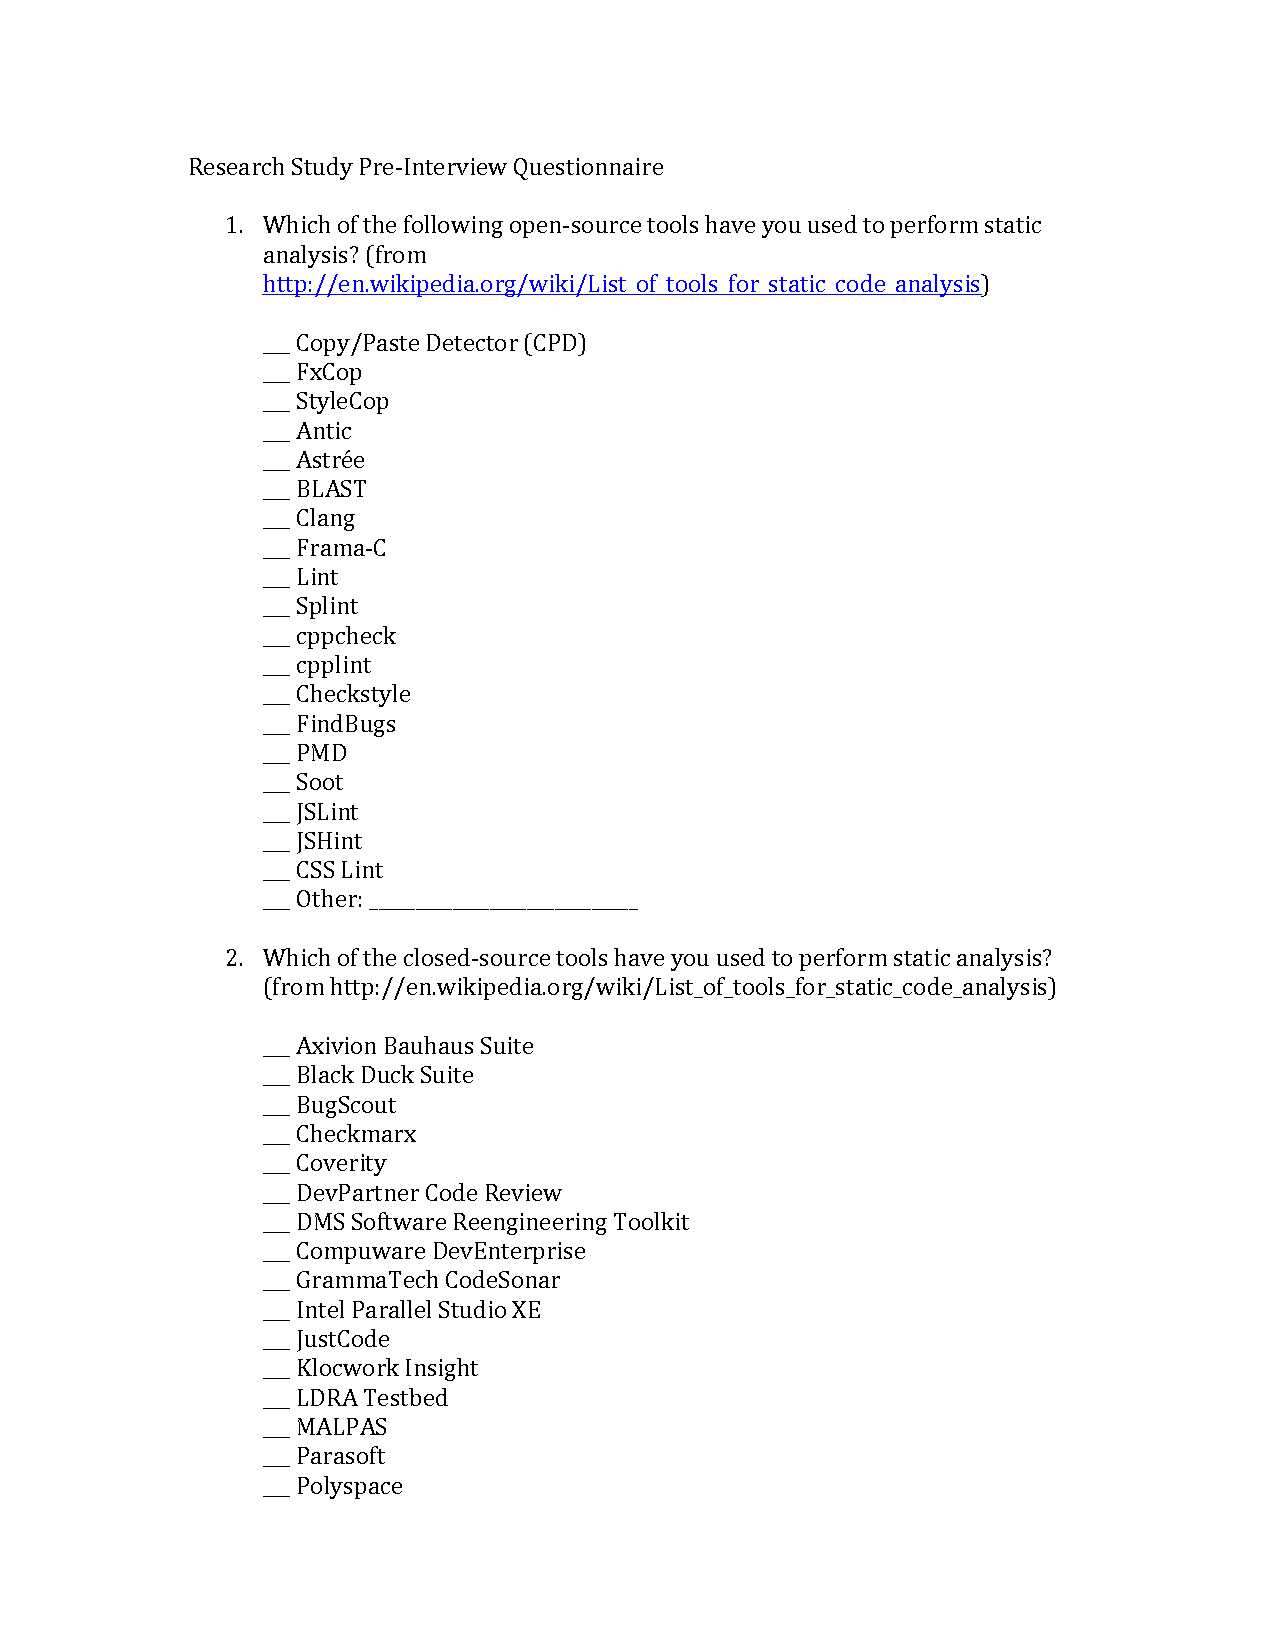
\includepdf[pages={1-},scale=0.70]{Chapter-3/figs/Pre-Int_Questionnaire.pdf}

\section{Interview Script}

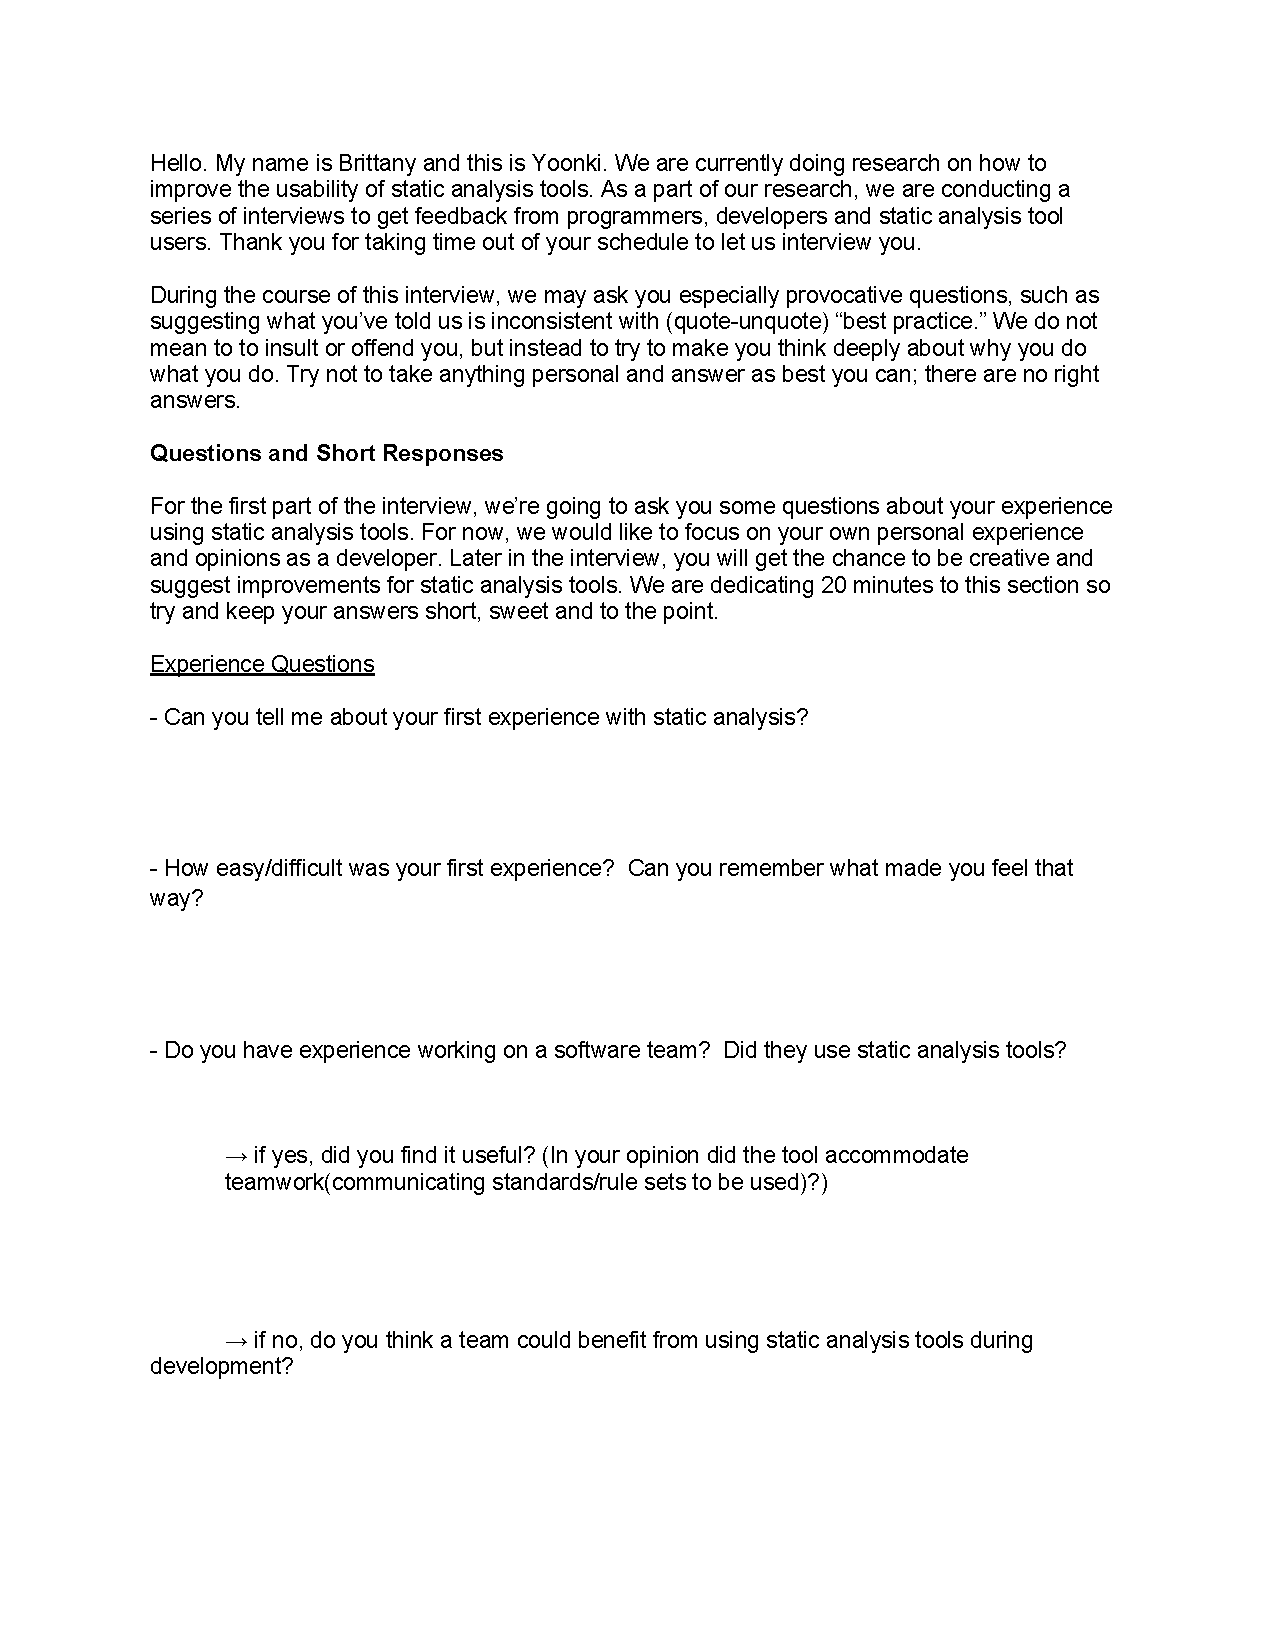
\includepdf[pages={1-},scale=0.60]{Chapter-3/figs/script.pdf}
% 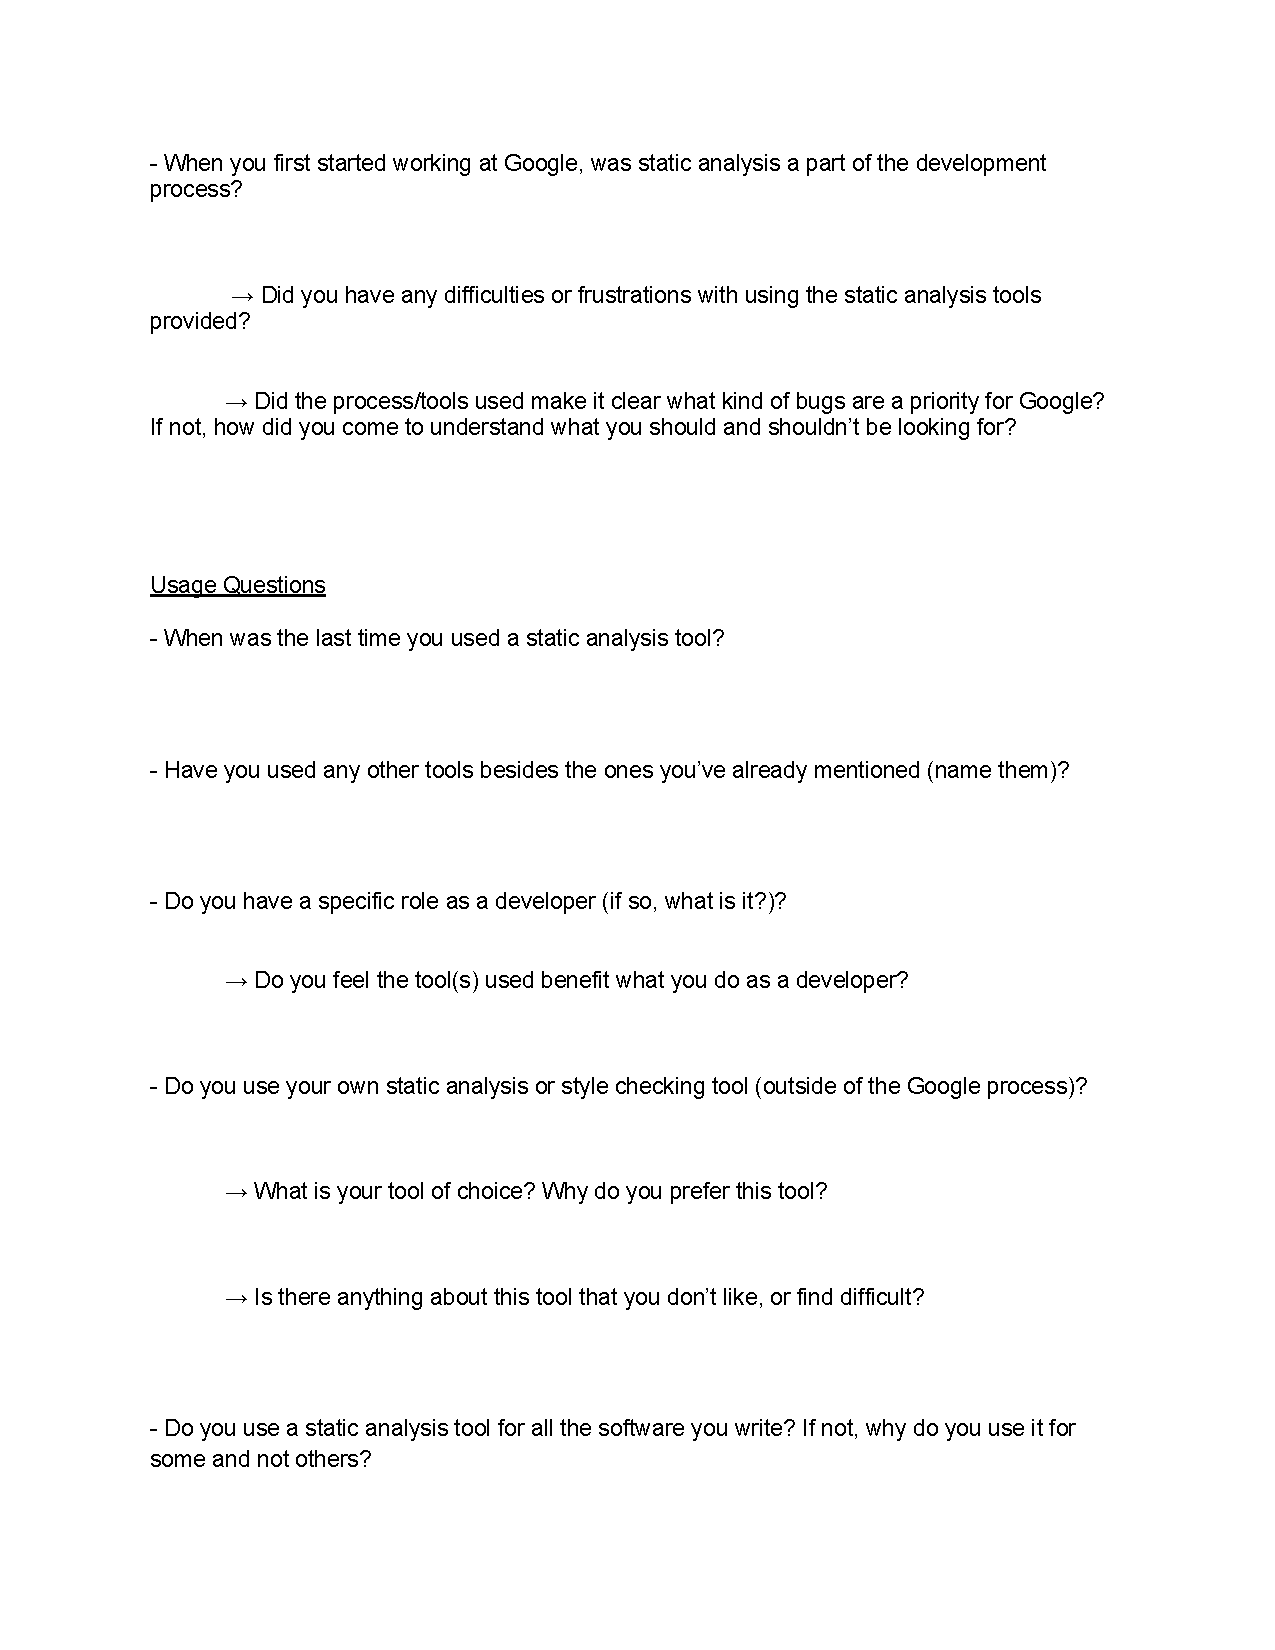
\includepdf[pages={1-},scale=0.60]{Chapter-3/figs/script-rest.pdf}

\section{Participatory Design Sketches}

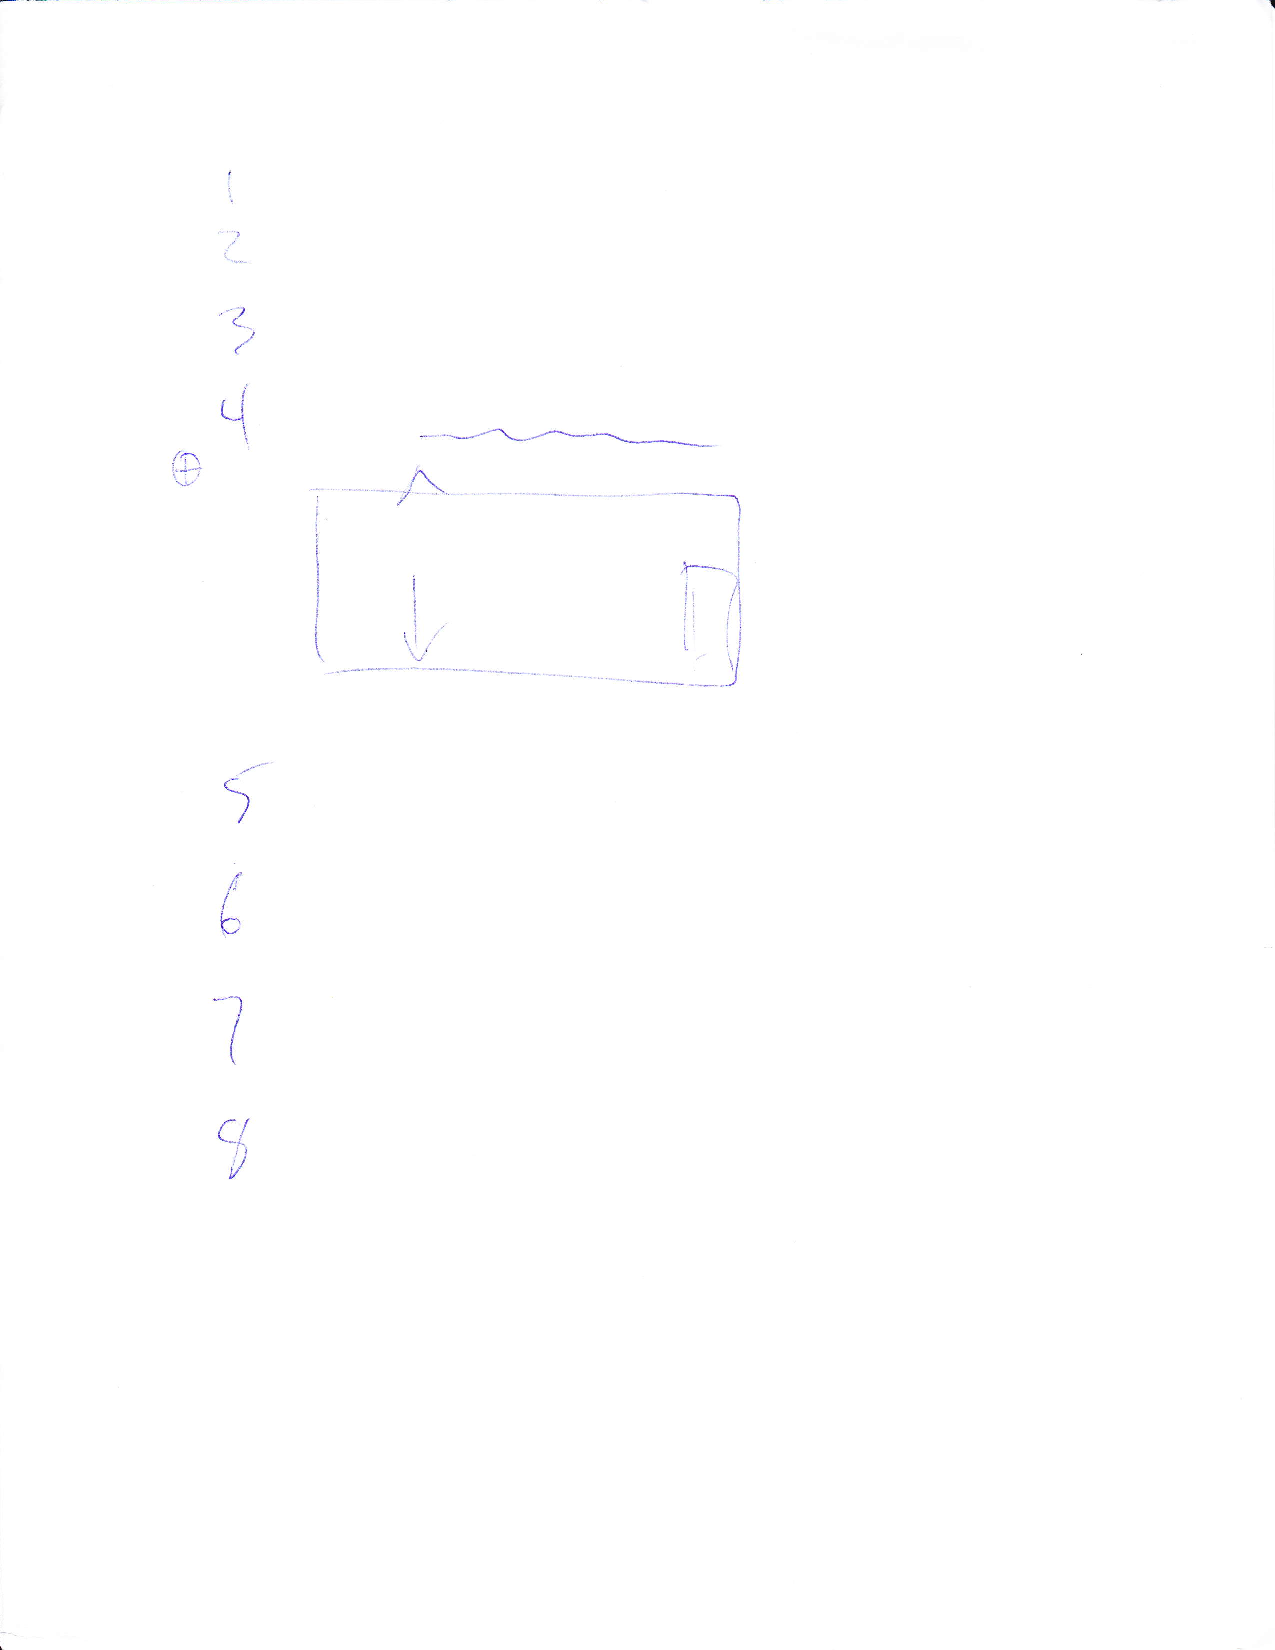
\includepdf[pages={1-},scale=0.60]{Chapter-3/figs/Sketches.pdf}
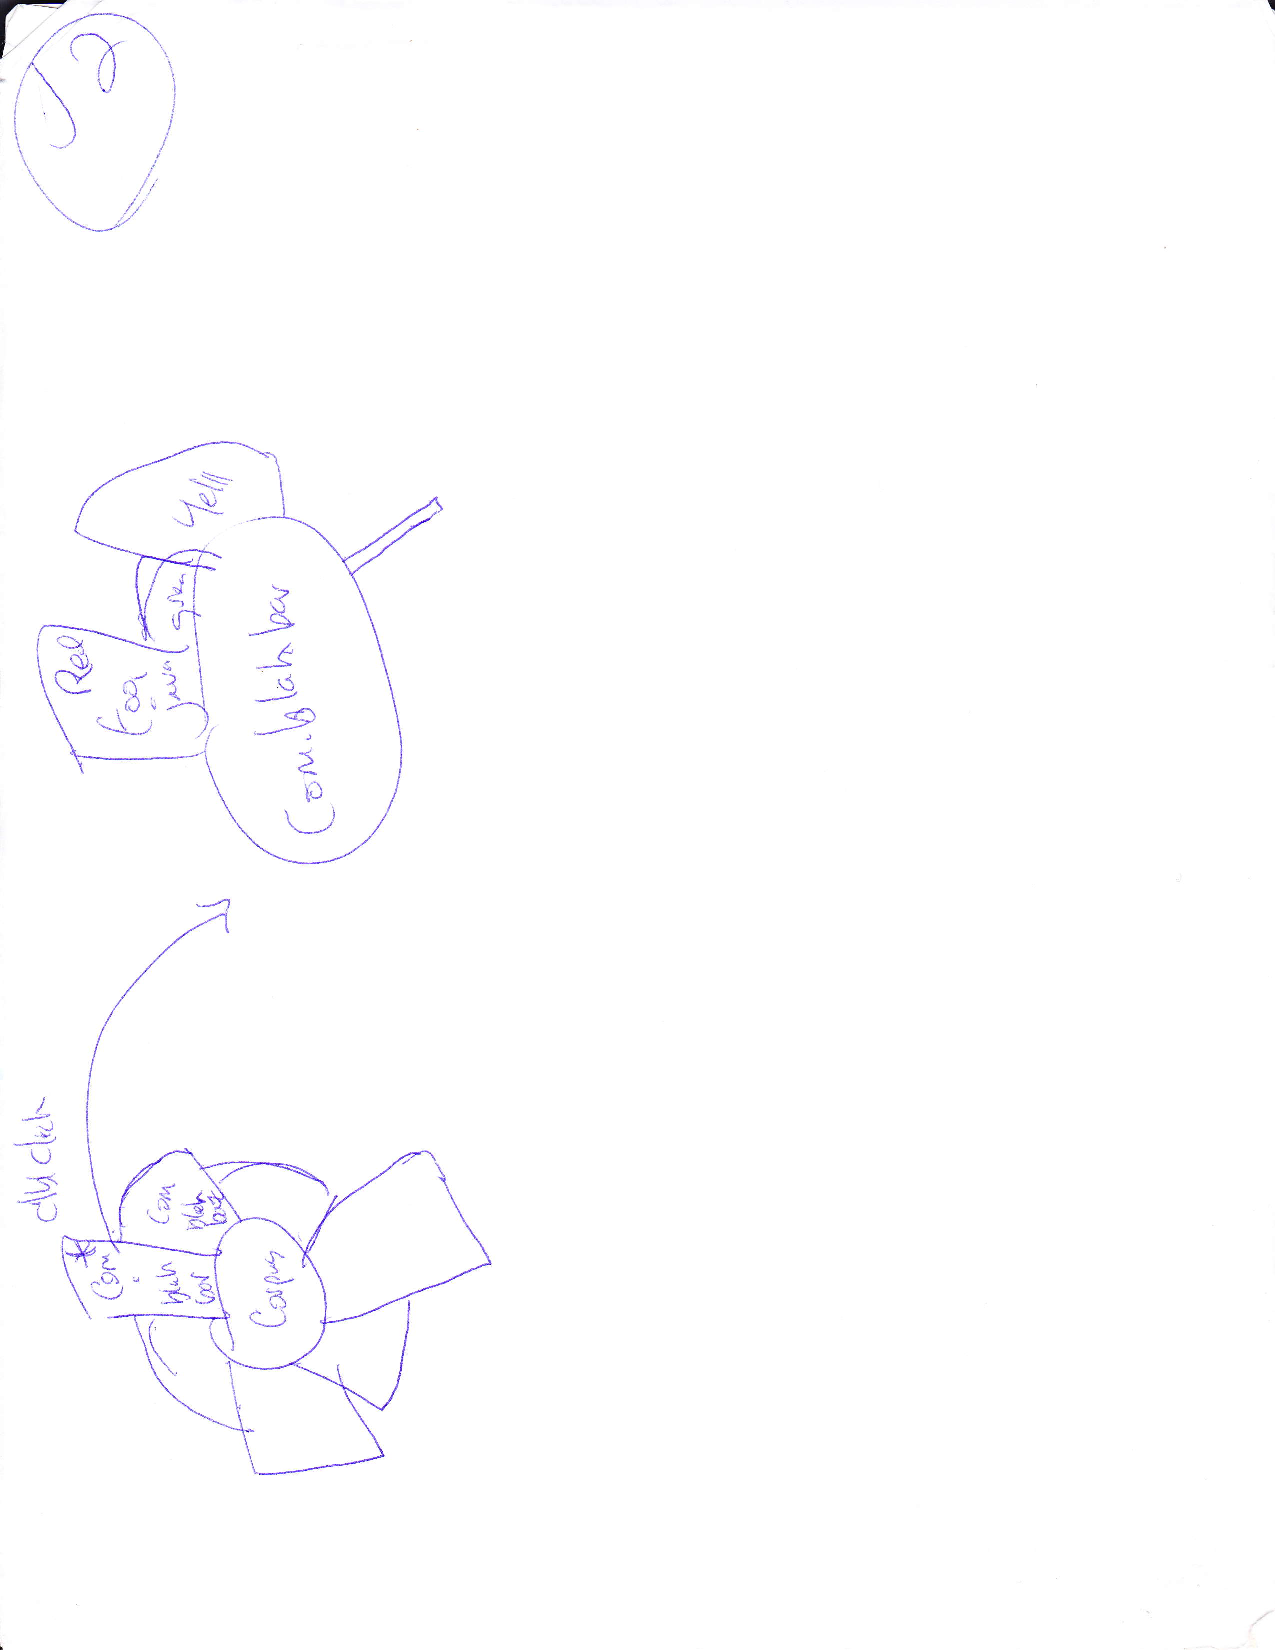
\includepdf[pages={1-},scale=0.60]{Chapter-3/figs/sketches-2.pdf}

\end{appendices}
\chapter{Chapter 4 Artifacts}\label{chap4:artifacts}

\begin{appendices}
    
    \section{Notification Oracle}
    
    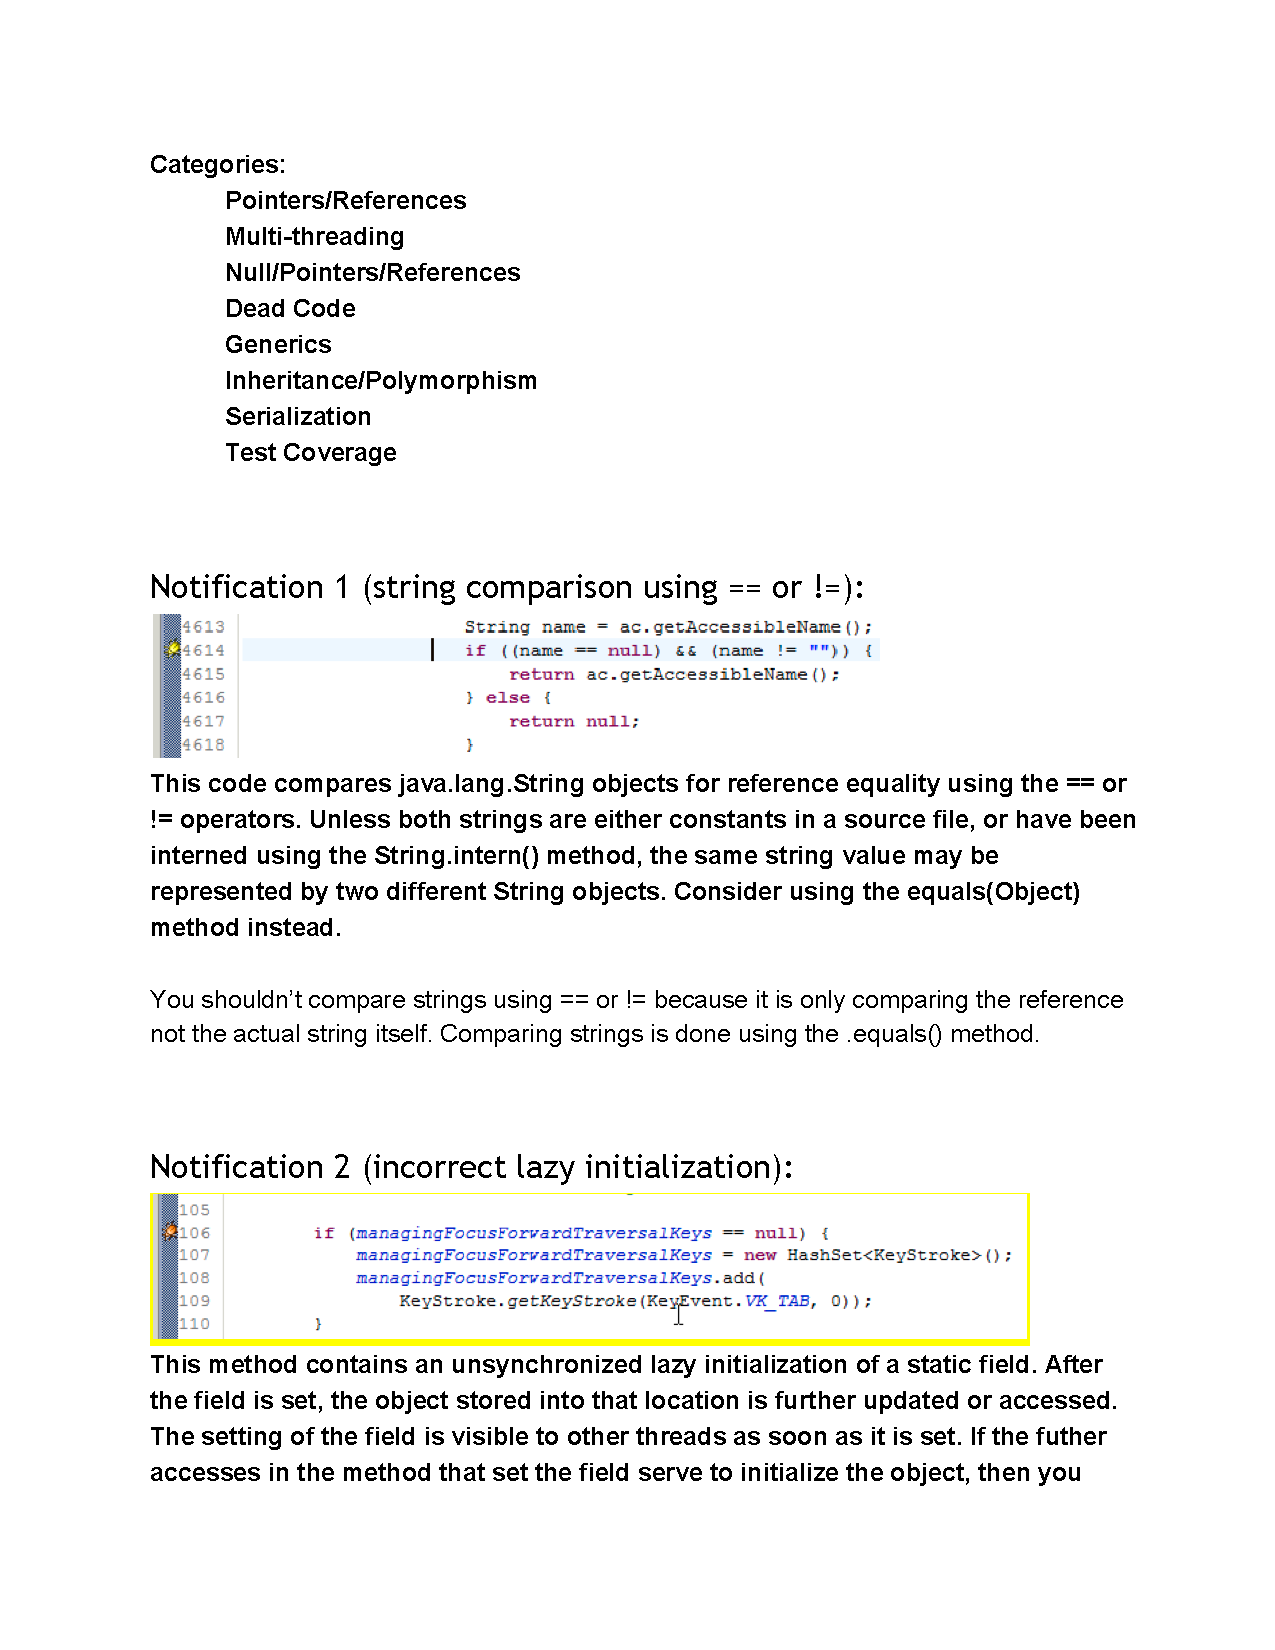
\includepdf[pages={1-},scale=0.70]{Chapter-4/figs/NotificationOracle.pdf}
    
    \section{Pre-Questionnaire and Consent Form}
    
    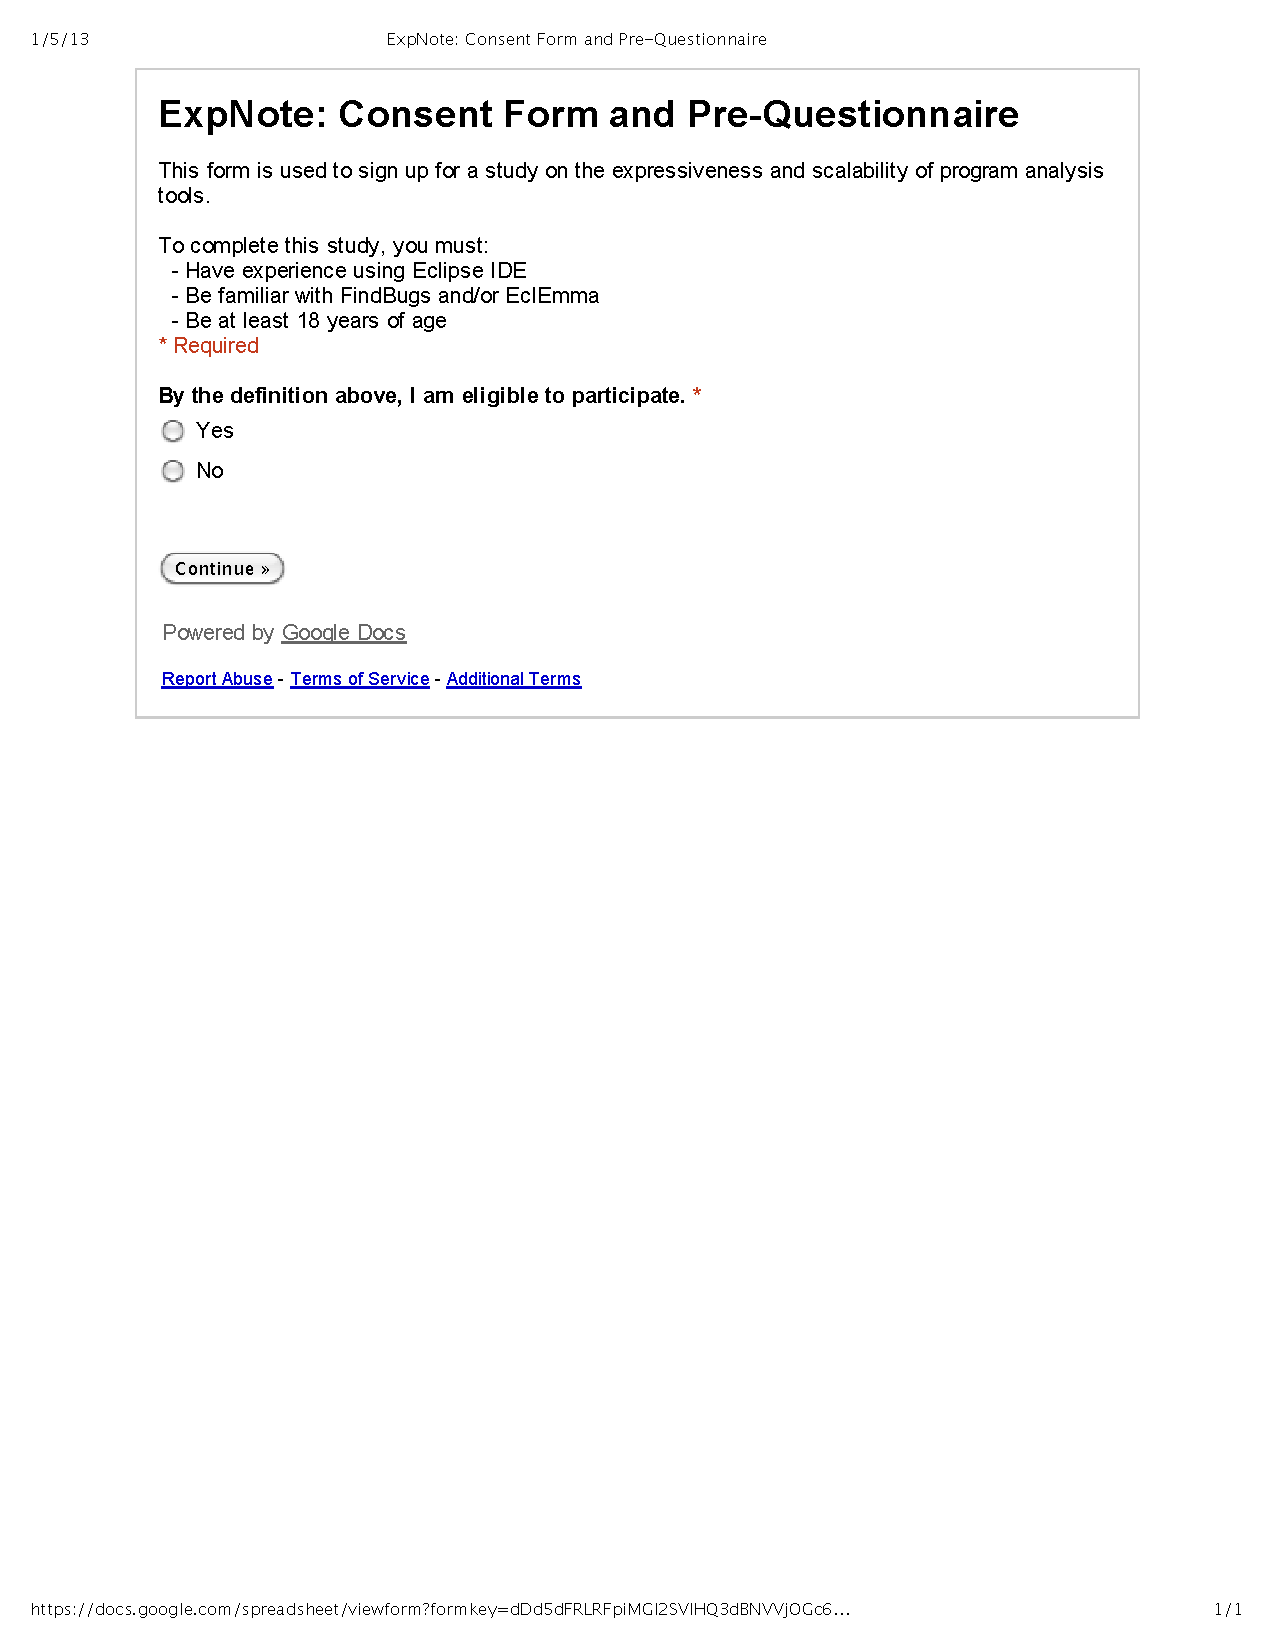
\includepdf[pages={1-},scale=0.70]{Chapter-4/figs/Consent.pdf}
    
    \section{Session Script}
    
    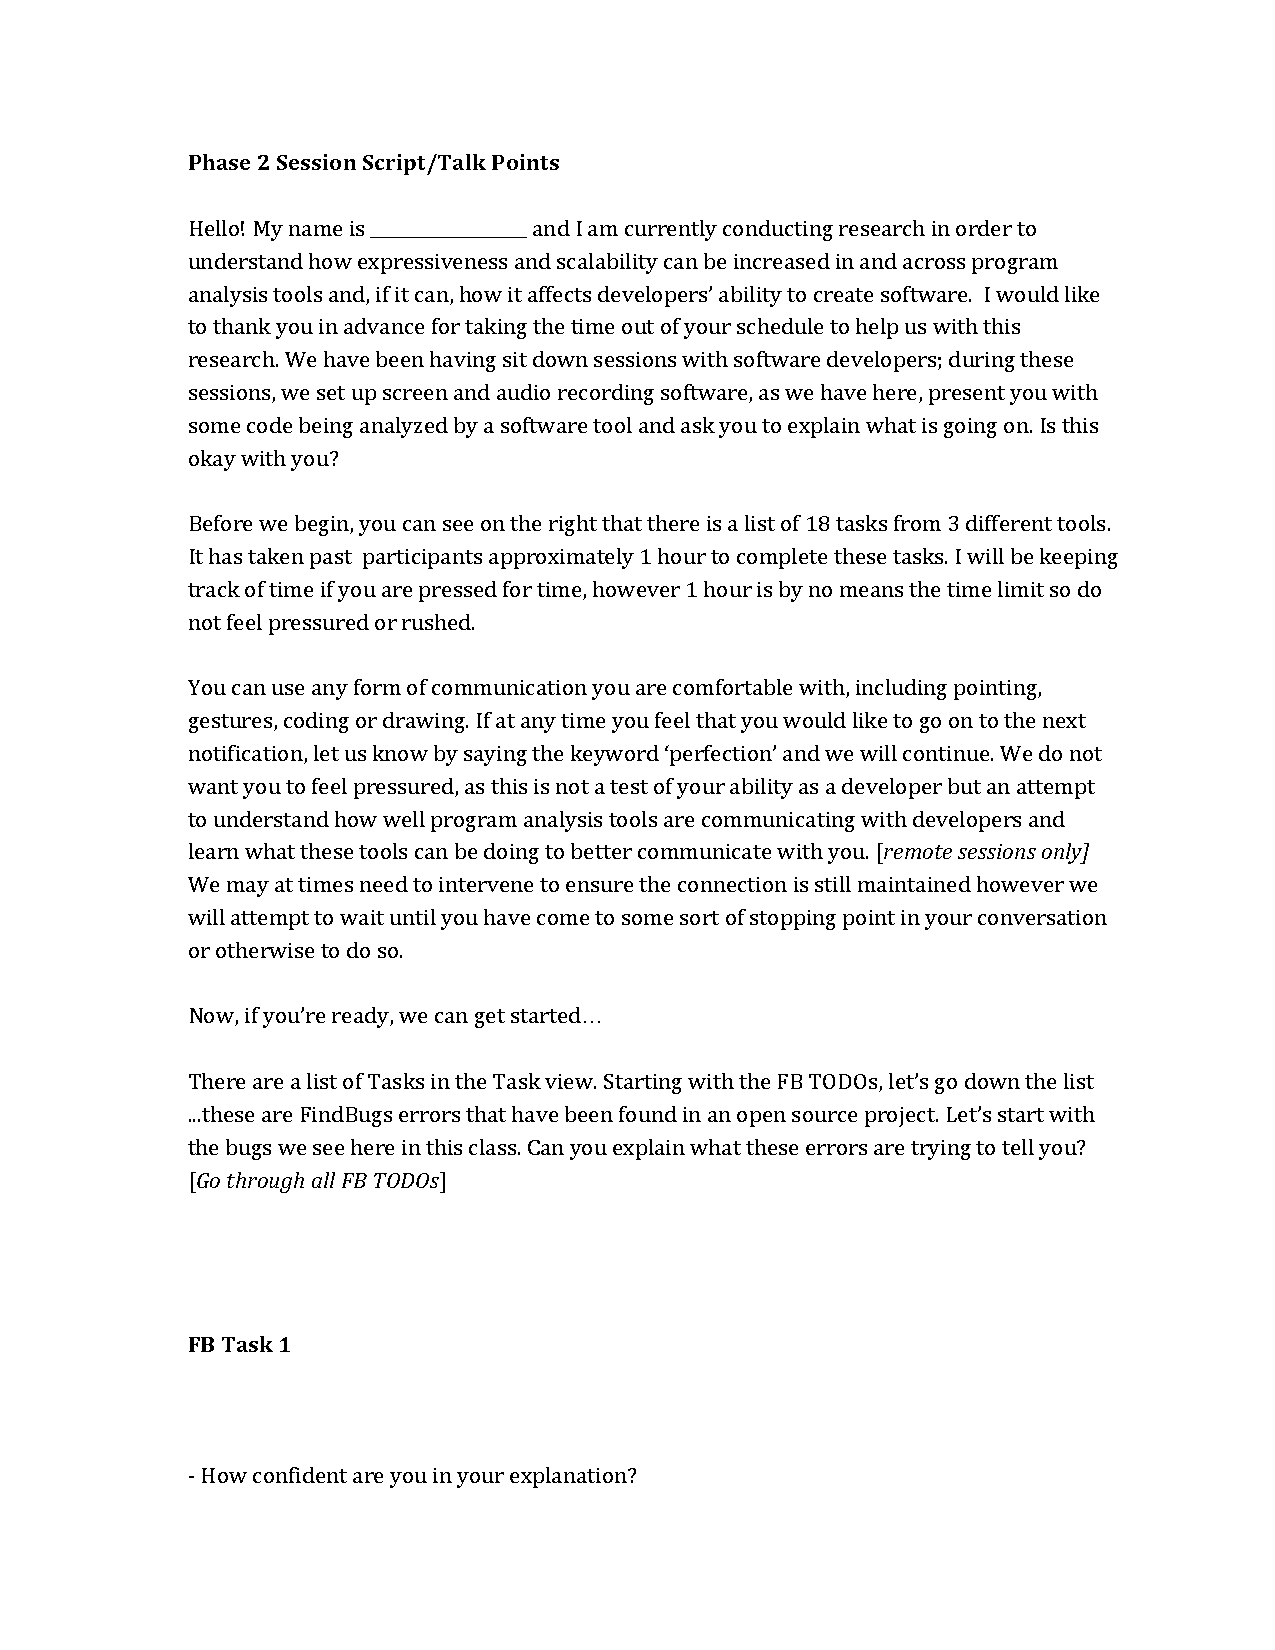
\includepdf[pages={1-},scale=0.70]{Chapter-4/figs/session-script.pdf}
    
\end{appendices}
%\chapter{Chapter 5 Artifacts}
\chapter{Chapter 6 Artifacts} \label{chap6:artifacts}

\begin{appendices}

    \section{Example Concept Inventory (Generics)}
    
    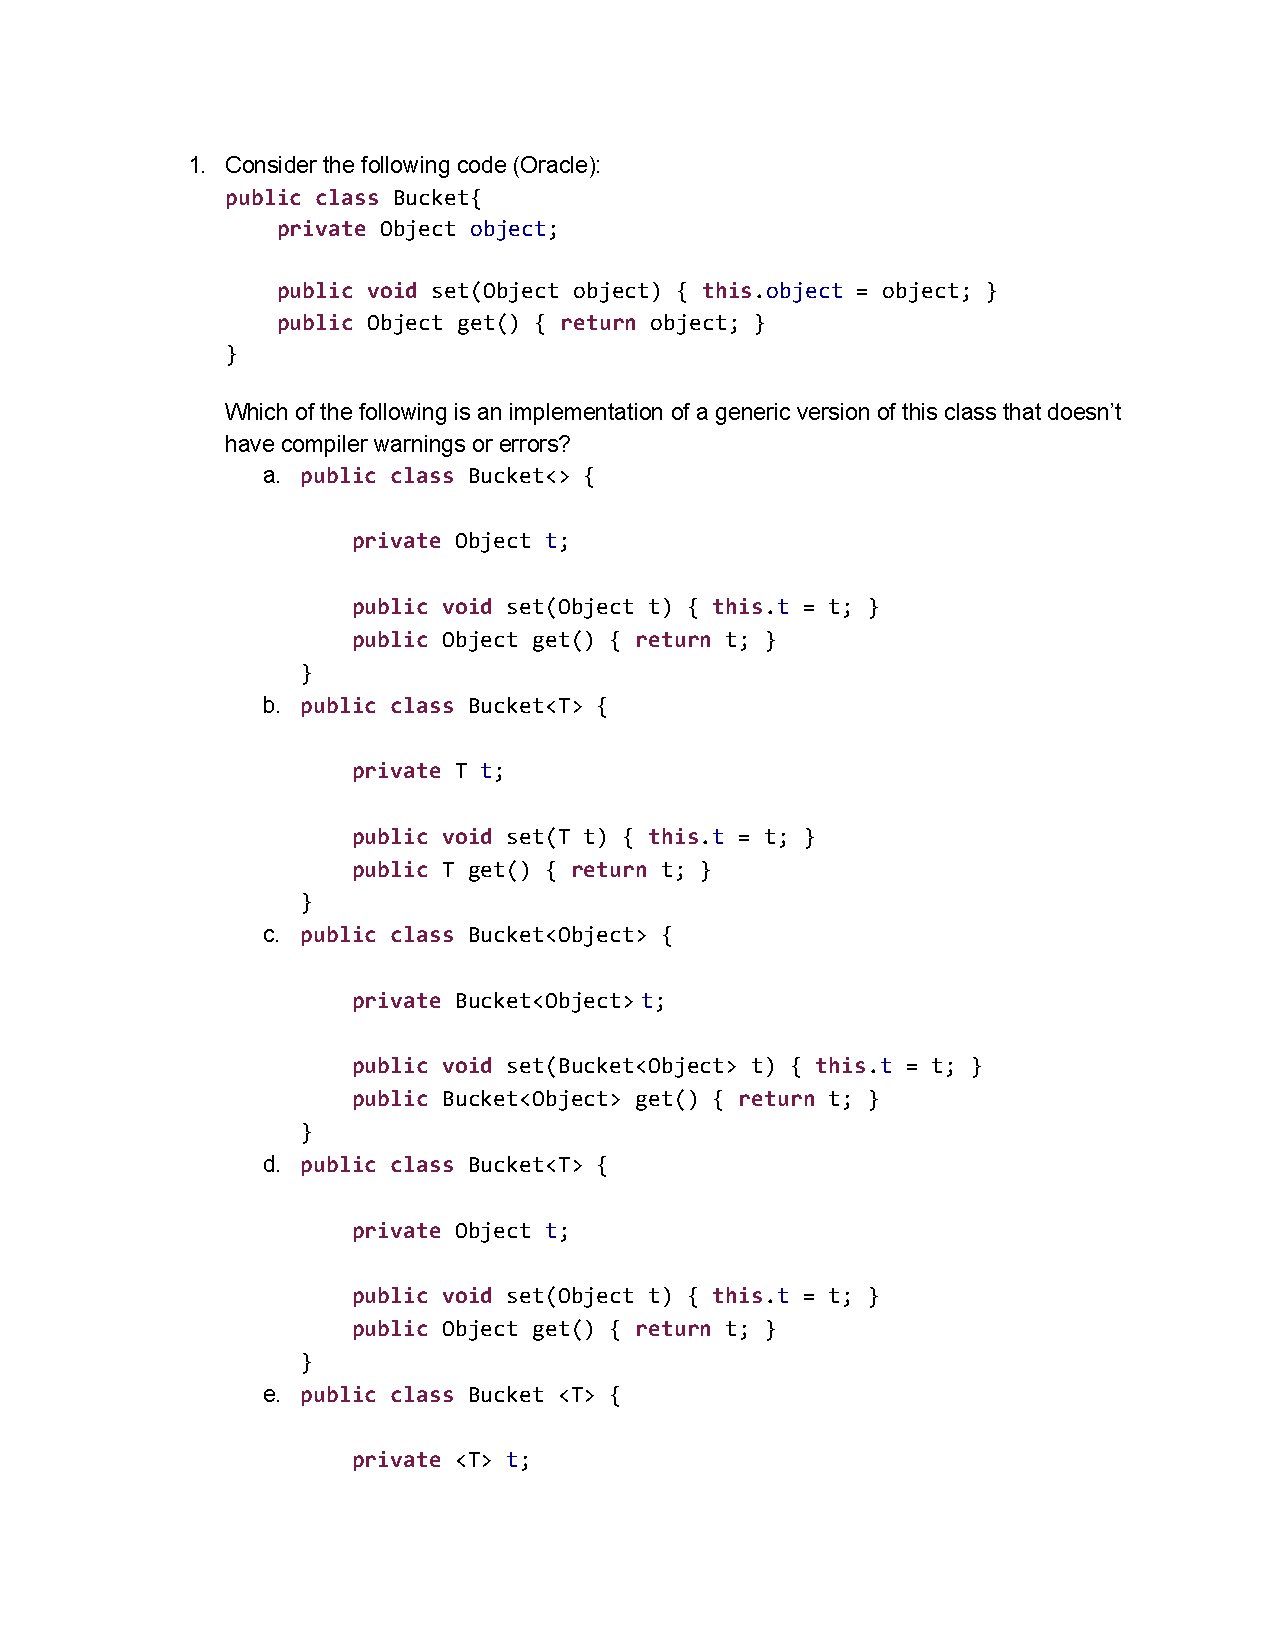
\includepdf[pages={1-},scale=0.70]{Chapter-6/figs/concept-inventory.pdf}
    
    \section{Example Feature Hierarchy (Generics)}
    
    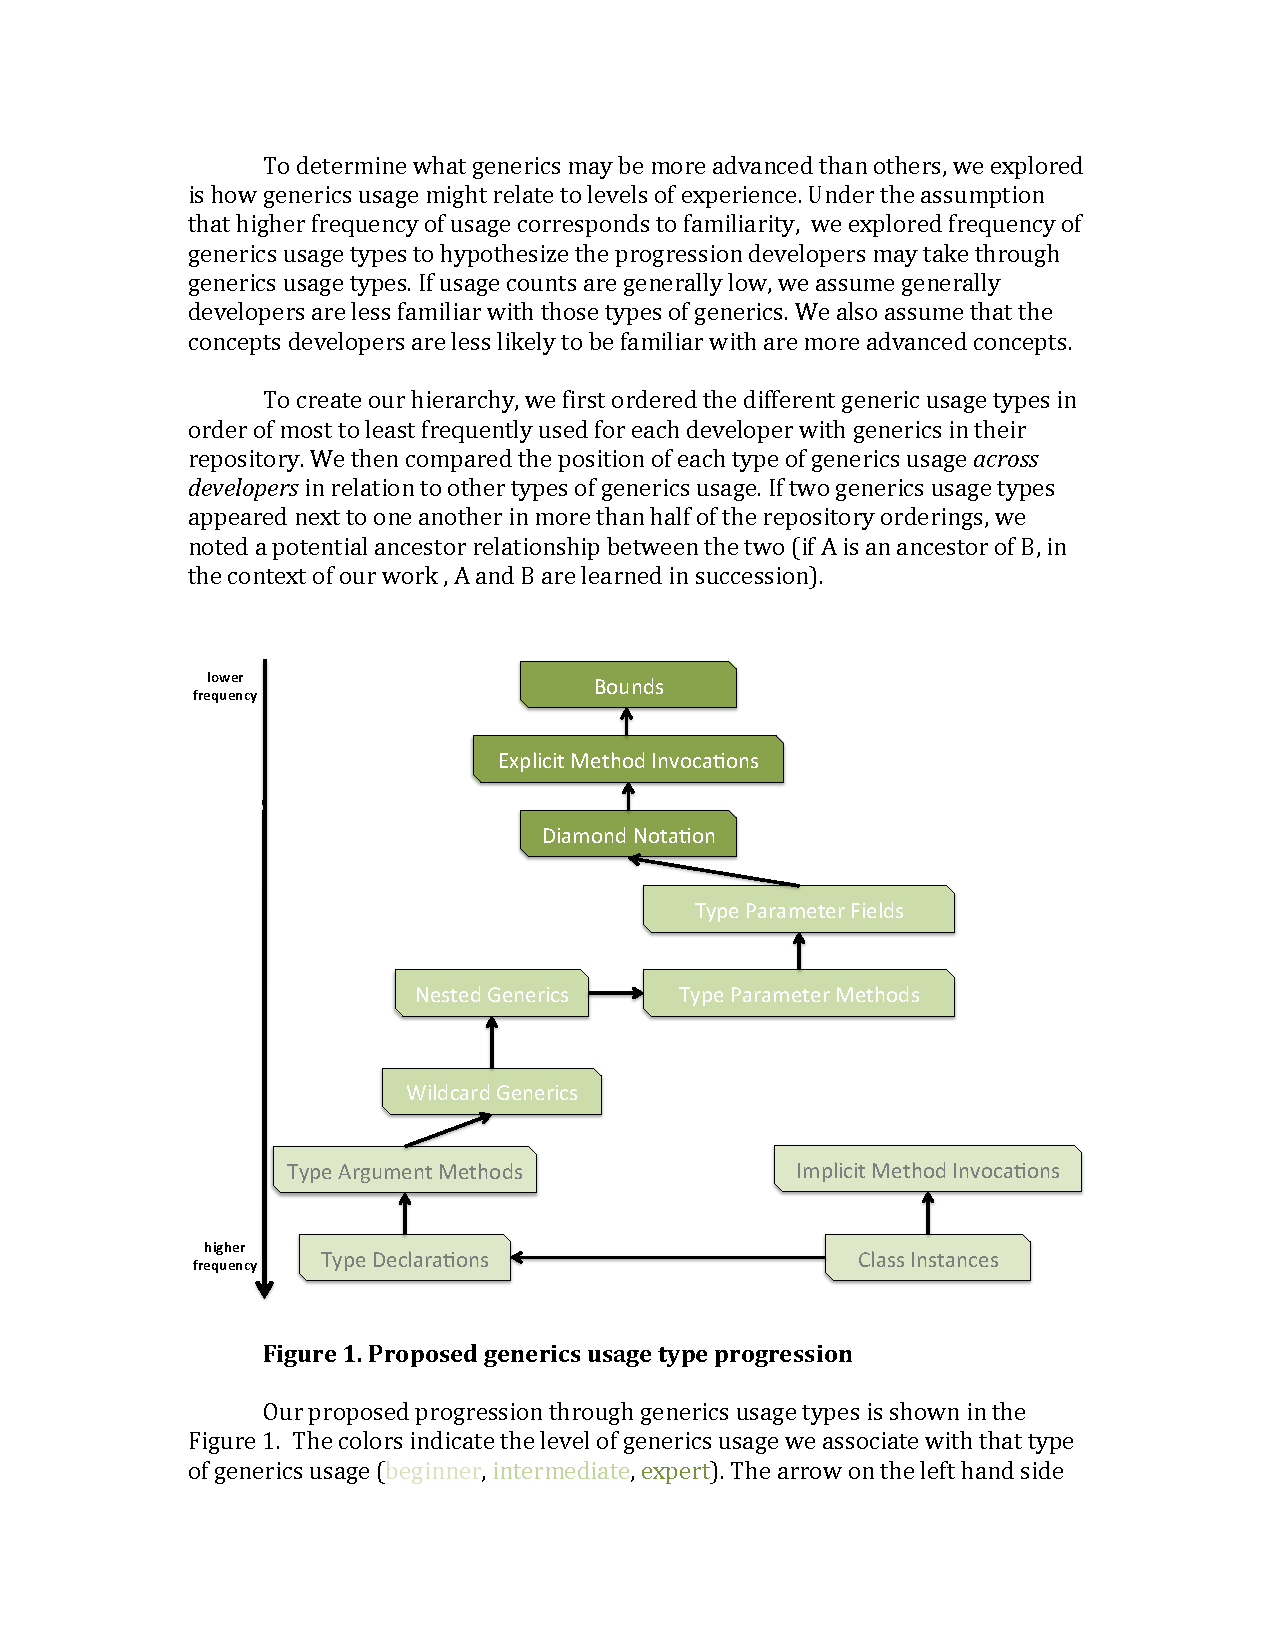
\includepdf[pages={1-},scale=0.70]{Chapter-6/figs/feature-map.pdf}
    
    \section{Example Concept Map and Bloom's Taxonomy Assessment Mapping (Generics)}
    
    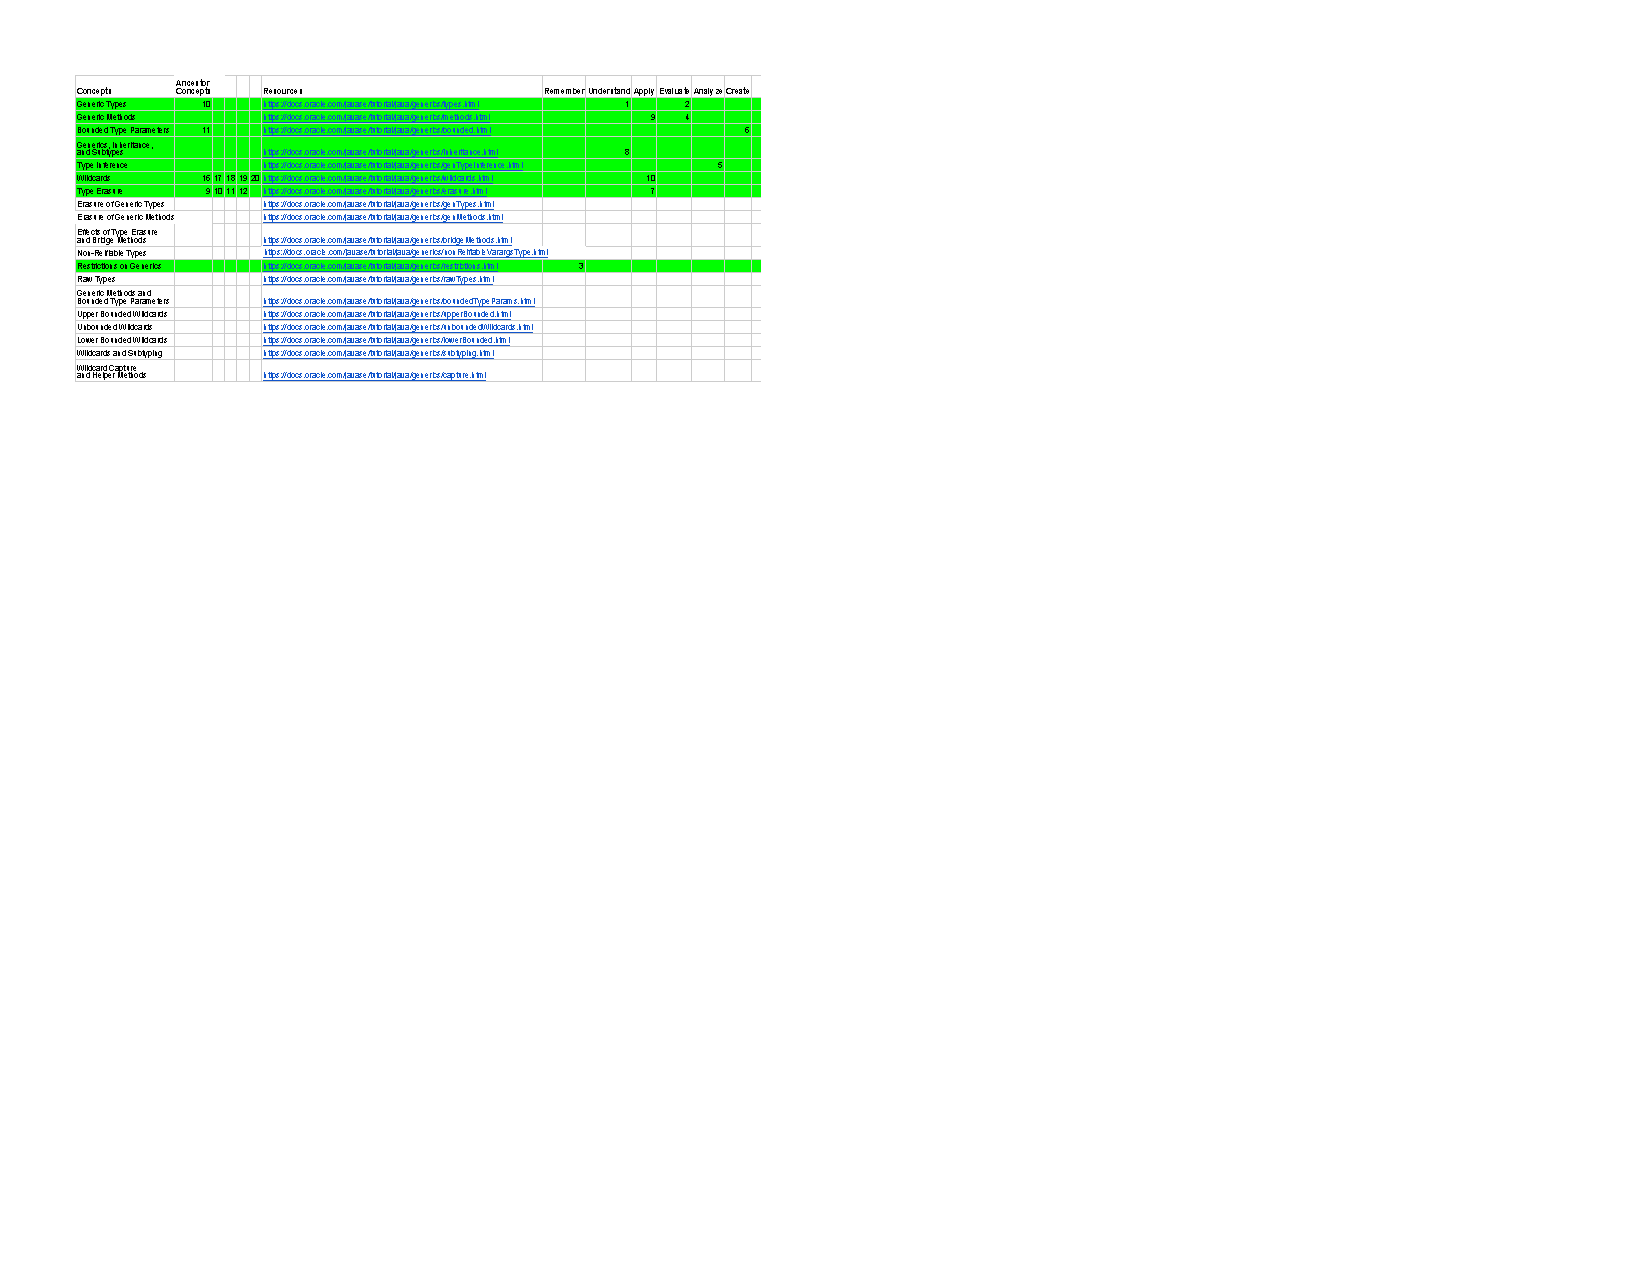
\includepdf[pages={1-},scale=0.70]{Chapter-6/figs/concept-graph.pdf}
    
\end{appendices}
\chapter{Chapter 7 Artifacts}

\restoregeometry

%%---------------------------------------------------------------------------%%
%\ensureoddstart
\backmatter


\end{document}
